%%%%%%%% ICML 2025 EXAMPLE LATEX SUBMISSION FILE %%%%%%%%%%%%%%%%%

\documentclass{article}

% Recommended, but optional, packages for figures and better typesetting:
\usepackage{microtype}
\usepackage{graphicx}
\usepackage{subfigure}
\usepackage{booktabs} % for professional tables

% hyperref makes hyperlinks in the resulting PDF.
% If your build breaks (sometimes temporarily if a hyperlink spans a page)
% please comment out the following usepackage line and replace
% \usepackage{icml2025} with \usepackage[nohyperref]{icml2025} above.
\usepackage{hyperref}
\usepackage{tikz}
\usepackage{pgfplots}
\usepackage{graphicx}
\usepackage{balance}
\usepackage{amssymb}
\usepackage[acronym]{glossaries}
\usepackage{xcolor}
% Define acronyms
\newacronym{VQ}{VQ}{vector quantizer}
\newacronym{SQ}{SQ}{scalar quantizer}
\newacronym{CL}{CL}{commitment loss}
\newacronym{STE}{STE}{straight-through estimator}
\newacronym{mSTE}{mSTE}{modified STE}
\newacronym{NA}{NA}{noise approximation}
\newacronym{MSE}{MSE}{mean-squared error}
\newacronym{MA-E}{MA-E}{mean-absolute embedding}
\newacronym{DAC}{DAC}{descript-audio-codec}
\usepgfplotslibrary{groupplots}
\usetikzlibrary{ positioning,shapes.geometric, arrows.meta, positioning, 3d, calc}
% Recommended, but optional, packages for figures and better typesetting:
\usepackage{microtype}
\usepackage{graphicx}
\usepackage{subfigure}
\usepackage{booktabs} % for professional tables
\usepackage{tikz}
\usetikzlibrary{shapes.geometric, arrows}
\usepackage{amsmath}
% hyperref makes hyperlinks in the resulting PDF.
% If your build breaks (sometimes temporarily if a hyperlink spans a page)
% please comment out the following usepackage line and replace
% \usepackage{icml2021} with \usepackage[nohyperref]{icml2021} above.
\usepackage{hyperref}

% Attempt to make hyperref and algorithmic work together better:
\newcommand{\theHalgorithm}{\arabic{algorithm}}

% Use the following line for the initial blind version submitted for review:
% If accepted, instead use the following line for the camera-ready submission:
\usepackage[accepted]{icml2025}

% For theorems and such
\usepackage{amsmath}
\usepackage{amssymb}
\usepackage{mathtools}
\usepackage{amsthm}

% if you use cleveref..
\usepackage[capitalize,noabbrev]{cleveref}

%%%%%%%%%%%%%%%%%%%%%%%%%%%%%%%%
% THEOREMS
%%%%%%%%%%%%%%%%%%%%%%%%%%%%%%%%
\theoremstyle{plain}
\newtheorem{theorem}{Theorem}[section]
\newtheorem{proposition}[theorem]{Proposition}
\newtheorem{lemma}[theorem]{Lemma}
\newtheorem{corollary}[theorem]{Corollary}
\theoremstyle{definition}
\newtheorem{definition}[theorem]{Definition}
\newtheorem{assumption}[theorem]{Assumption}
\theoremstyle{remark}
\newtheorem{remark}[theorem]{Remark}

% Todonotes is useful during development; simply uncomment the next line
%    and comment out the line below the next line to turn off comments
%\usepackage[disable,textsize=tiny]{todonotes}
\usepackage[textsize=tiny]{todonotes}


% The \icmltitle you define below is probably too long as a header.
% Therefore, a short form for the running title is supplied here:
\icmltitlerunning{Efficient Evaluation of Quantization-Effects in Neural Codecs}

\begin{document}

\twocolumn[
\icmltitle{Efficient Evaluation of Quantization-Effects in Neural Codecs}

% It is OKAY to include author information, even for blind
% submissions: the style file will automatically remove it for you
% unless you've provided the [accepted] option to the icml2025
% package.

% List of affiliations: The first argument should be a (short)
% identifier you will use later to specify author affiliations
% Academic affiliations should list Department, University, City, Region, Country
% Industry affiliations should list Company, City, Region, Country

% You can specify symbols, otherwise they are numbered in order.
% Ideally, you should not use this facility. Affiliations will be numbered
% in order of appearance and this is the preferred way.

\begin{icmlauthorlist}
\icmlauthor{Wolfgang Mack}{yyy}
\icmlauthor{Ahmed Mustafa}{yyy}
\icmlauthor{Rafał Łaganowski}{yyy}
\icmlauthor{Samer Hijazy}{yyy}
\end{icmlauthorlist}

\icmlcorrespondingauthor{Wolfgang Mack}{womack@cisco.com}
\icmlaffiliation{yyy}{Cisco Systems, Inc., \{womack, ahmmusta, rlaganow, hijazy\}@cisco.com}


\vskip 0.3in
]

% this must go after the closing bracket ] following \twocolumn[ ...

% This command actually creates the footnote in the first column
% listing the affiliations and the copyright notice.
% The command takes one argument, which is text to display at the start of the footnote.
% The \icmlEqualContribution command is standard text for equal contribution.
% Remove it (just {}) if you do not need this facility.

\printAffiliationsAndNotice{}  % leave blank if no need to mention equal contribution
%\printAffiliationsAndNotice{\icmlEqualContribution} % otherwise use the standard text.
\begin{abstract}

Neural codecs, comprising an encoder, quantizer, and decoder, enable signal transmission at exceptionally low bitrates. Training these systems requires techniques like the straight-through estimator, soft-to-hard annealing, or statistical quantizer emulation to allow a non-zero gradient across the quantizer. Evaluating the effect of quantization in neural codecs, like the influence of gradient passing techniques on the whole system, is often costly and time-consuming due to training demands and the lack of affordable and reliable metrics. This paper proposes an efficient evaluation framework for neural codecs using simulated data with a defined number of bits and low-complexity neural encoders/decoders to emulate the non-linear behavior in larger networks. Our system is highly efficient in terms of training time and computational and hardware requirements, allowing us to uncover distinct behaviors in neural codecs. We propose a modification to stabilize training with the straight-through estimator based on our findings. We validate our findings against an internal neural audio codec and against the state-of-the-art descript-audio-codec.

\end{abstract}

\section{Introduction}
\label{submission}
Codec systems typically consist of an encoder, a quantizer, and a decoder. The encoder transforms high-dimensional data such that it can be quantized, i.e. represented with a typically much smaller number of discrete values. Storing or transmitting data in the quantized representation is crucial in modern multi-media environments as it significantly reduces storage and transmission requirements and typically does not reduce perceived quality like audio clarity or video sharpness significantly (e.g., \cite{4604423,muller24c_interspeech}).  Subsequently, the decoder reconstructs the data from the quantized representations. 

 Classical coding methods, such as JPEG \cite{jpegstandard}, MP3 \cite{mp3}, H.264 \cite{h264}, and  Opus \cite{opus} are based on signal processing and perceptual models  \cite{SpeechCodingBase,bhaskaran1995image}. Despite their historical success, these techniques struggle to achieve high efficiency at very low bitrates, where signal fidelity becomes a critical challenge (e.g., \cite{Zeghidour2022}).

With the rise of deep learning, classical methods have been combined with neural networks. Neural vocoders, for example, have been employed to reconstruct high-fidelity signals from bitstreams of classical methods, achieving unprecedented performance in speech and audio compression \cite{Kleijn2018, Klejsa2019, Garbacce2019,  Valin2019a,9632750}. Neural networks are also used as post-processing tools to mitigate compression artifacts, thereby enhancing the perceptual quality of the decoded signals \cite{Zhao2019, Korse2020, Biswas2020, Korse2022, Buthe2024}. 

End-to-end neural compression systems that bypass traditional coding elements have emerged as an alternative. These systems learn to encode, quantize, and decode signals directly from data and can be trained end-to-end \cite{ VanDenOord2017,  balle2016endtoend,Agustsson2019,Zeghidour2022, Defossez2022, NSVQ,Vali2023,  Kumar2023, Ai2024, Mentzer2024, Brendel2024}. However, training such systems requires tricks like the straight-through estimator \cite{VanDenOord2017,bengio2013ste}, soft-to-hard annealing \cite{agustsson2017soft,Jang2017,maddison2017gumbel}, or statistical quantizer emulation \cite{balle2016endtoend,9242247,NSVQ,Vali2023,Brendel2024} to allow a non-zero gradient to pass over the quantizer.  

Evaluating neural codecs is nontrivial, costly, and time-consuming because of the required training and is often not practical because of the lack of cheap and reliable metrics. Evaluation points for neural codecs, such as quantization error or decoder output, face challenges due to the non-linear systems involved. For example, a small quantization error can lead to a significant reconstruction error and vice versa. Metrics for assessing decoder outputs in the audio, image, or video domains are often either subjective and resource-intensive or objective but unreliable. For example, MUSHRA (Multiple Stimuli with Hidden Reference and Anchor) is a subjective evaluation method widely regarded as the gold standard for audio quality assessment. Although highly effective in capturing perceptual quality, MUSHRA tests require human participants, limiting their scalability to a small number of files and increasing the associated costs. Furthermore, MUSHRA scores often show limited correlation with objective metrics, a disparity that becomes particularly pronounced when evaluating generative models such as neural codecs.

\begin{figure}[t]
    \centering
    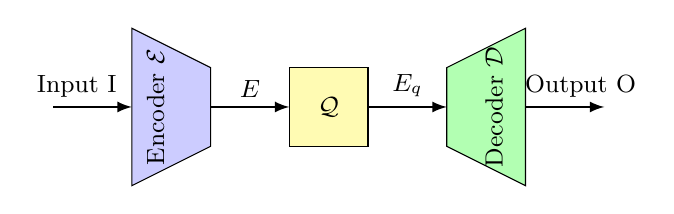
\begin{tikzpicture}[>=latex, font=\small]

        % Encoder (shrinks in height)
        \draw[fill=blue!20] (-4, 1) -- (-3, 0.5) -- (-3, -0.5) -- (-4, -1) -- cycle;
        \node[rotate=90] at (-3.7, 0) {Encoder $\mathcal{E}$};

        % Quantizer (Q)
        \draw[fill=yellow!30] (-2, 0.5) rectangle (-1, -0.5);
        \node at (-1.5, 0) {$\mathcal{Q}$};

        % Decoder (expands in height)
        \draw[fill=green!30] (0, 0.5) -- (1, 1) -- (1, -1) -- (0, -0.5) -- cycle;
        \node[rotate=90] at (0.6, 0) {Decoder $\mathcal{D}$};

        % Input and output labels above arrows
        \node[above] at (-4.7, 0) {Input I};
        \node[above] at (1.7, 0) {Output O};

        % Labels for arrows
        \node[above] at (-2.5, 0) {$E$};         % Label after Encoder
        \node[above] at (-0.5, 0) {$E_q$}; % Label after Quantizer

        % Arrows with equal spacing
        \draw[->, thick] (-5, 0) -- (-4, 0);    % Input arrow
        \draw[->, thick] (-3, 0) -- (-2, 0);    % Arrow Encoder to Q
        \draw[->, thick] (-1, 0) -- (0, 0);     % Arrow Q to Decoder
        \draw[->, thick] (1, 0) -- (2, 0);      % Arrow after Decoder

    \end{tikzpicture}
    \caption{A neural codec system with an encoder $(\mathcal{E})$ mapping the input to embeddings $E$, a quantizer ($\mathcal{Q}$) mapping $E$ to the quantized version $E_q$. The decoder $(\mathcal{D})$ maps $E_q$ to the output. }
    \label{fig:neural_codec}
\end{figure}
In this paper, we propose an evaluation framework that enables efficient investigation and evaluation of quantizers in neural codecs in a controlled way. The proposed framework consists of a simple input and target data simulation method to train a neural codec. The input data is designed to have a specified number of bits. Designing the data in that way enables the identification of the minimum number of bits required by the quantizer to reconstruct the target perfectly. The target is a rotated input version containing the same number of bits. The input and target data design are based on quantized noise processes, which ensures a resource-efficient, low-cost simulation framework. In addition to the data simulation, we propose to use a low-complexity neural codec. That way, we emulate the highly non-linear behavior before and after the quantizer in a large network by simultaneously keeping hardware requirements and training cost/time extremely low. For training the neural codec, we propose to use an interpretable cost function like the \gls{MSE} between target and estimate to evaluate the quantizer performance. The proposed loss is in contrast to real codecs, where the estimate is hard to assess regarding quality. Using the proposed framework, we evaluate fundamental properties of neural codecs by comparing training using statistical quantizer emulation to training using the \gls{STE} with and without  \gls{CL}. We find similarities between both approaches and propose a modification to stabilize training with the \gls{STE}. Finally, we verify our findings by repeating selected experiments with an internal audio codec and \gls{DAC} \cite{Kumar2023}.   

The remainder of the paper is structured as follows. Fundamental mathematical notations are introduced in Section~\ref{sec:fundamentals}. The proposed method is presented in Section~\ref{sec:prop}, followed by the experimental parameters in Section~\ref{sec:paras}. In Section~\ref{sec:Peval}, experiments are covered. Finally, Section~\ref{sec:conclusion} contains a brief conclusion.
\section{Fundamentals}
\label{sec:fundamentals}

We consider an encoder-quantizer-decoder system, as illustrated in Figure~\ref{fig:neural_codec}. The encoder $\mathcal{E}$ maps the input $I$ to embeddings $E \in \mathbb{R}^{F \times N}$, where $F$ represents the feature dimension and $N$ the frame dimension. A quantization module $\mathcal{Q}$ then maps $E$ to its quantized form $E_q$. Finally, the decoder $\mathcal{D}$ processes $E_q$ to estimate the output $O$. Depending on the application, $I$ and $O$ could be images, audio, or other signals. Without loss of generality, we refrain from specifying the exact nature of these signals. Instead, we focus on analyzing the quantization module $\mathcal{Q}$ and its effects on the neural codec. In particular, we examine its influence on the relationship between $E$ and $E_q$, as well as the gradient flow through $\mathcal{Q}$\footnote{Note that $\mathcal{Q}$ is embedded in the highly non-linear encoder-decoder system. Consequently, analyzing quantizers in the form of their quantization error is insufficient to evaluate their performance in neural networks, as a small quantization error might lead to a large output error and vice versa. }.

The gradient flow over $\mathcal{Q}$ poses a fundamental challenge: in most quantizer designs, $\mathcal{Q}$ is non-differentiable because it maps nearly continuous embeddings $E$ to discrete values or vectors in $E_q$. This non-differentiability prevents loss functions defined after $\mathcal{Q}$ from directly updating the encoder weights. Various techniques have been proposed to overcome this limitation,  including (1) the \gls{STE} \cite{VanDenOord2017,bengio2013ste}, (2) statistical training using noise-based approximations for the quantization error \cite{balle2016endtoend,9242247,NSVQ,Vali2023,Brendel2024}, and (3) soft quantization \cite{agustsson2017soft,Jang2017,maddison2017gumbel}.
\begin{figure}[t]
    \centering
    \newsavebox\myboxa
    \savebox\myboxa{%
    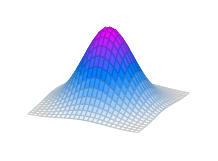
\begin{tikzpicture}
    \begin{axis}[scale=0.3,
        hide axis,
        colormap/cool,title style={yshift=-0.8cm}, zmin=0, zmax=1]
        \addplot3[surf,domain=-3:3,domain y=-3:3,] 
            {exp(-( (x)^2 + (y)^2)/3 )};
    \end{axis}
    \end{tikzpicture}%
    }

    % The block diagram code is probably more verbose than necessary
    \begin{tikzpicture}
    \tikzstyle{branch}=[fill,shape=circle,minimum size=3pt,inner sep=0pt]
    % Draw blocks, inputs, and outputs
    \node[label={[label distance=-0.5cm]above:{$I \in \mathbb{R}^{P\times P}$}}] (input) {\usebox\myboxa};
    
    % Sampling (rotate the box 90 degrees)
    \node[draw, rectangle, right=of input] (Sample) {\rotatebox{90}{Sampling}};
    
    % Scalar Quantization (rotate the box 90 degrees)
    \node[draw, rectangle,  right=of Sample] (Q) {\rotatebox{90}{Scalar Quantization}};
    
    % Circle with dot
    \node[right=of Q, circle, draw] (o1) {$\odot$}; % First multiplication dot
    \node[above= of o1] (rot) {Rotation Matrix $Q$};
    \node[right=of o1] (o2) {}; % Second multiplication dot

    % Arrows connecting blocks and circles
    \draw[->] (input) -- (Sample) ;  % Arrow from input to Sampling
    \draw[->] (Sample) -- (Q) node[above,midway]{$X$};  % Arrow from Sampling to Scalar Quantization
    \draw[->] (Q) -- (o1) node[above,midway]{$X_q$}; % Arrow from Scalar Quantization to first dot
    \draw[->] (o1) -- (o2)node[above,midway]{$Y$};;  % Arrow from first dot to second dot
    \draw[->] (rot) -- (o1); % Arrow from rotation matrix to first dot
    \end{tikzpicture}
       \caption{Proposed data generation pipeline. A Gaussian noise process with a $P\times P$ identity covariance matrix is sampled to obtain $X$. Each element in $X$ is quantized via scalar quantization to obtain the network target $X_q$. A rotation matrix is applied to $X_q$ to obtain the network input $Y$.  }
    \label{fig:datagen}
\end{figure}

In the case of the \gls{STE}, the decoder input $\mathcal{D}^{\text{STE}}_{\text{in}}$ during training is defined as
\begin{equation}
\mathcal{D}^{\text{STE}}_{\text{in}} = E + \text{sg}[\underbrace{E_q - E}_{Q_e}],
\label{equ:STE}
\end{equation}
where $Q_e$ is the quantization error, and $\text{sg}[\bullet]$ stops gradient tracking for $\bullet$ \footnote{Note that  $\text{sg}[(E_q-E)]$ is crucial, without it the decoder input would be $E_q = E +(E_q-E)$ which has gradients of $0$ w.r.t. $E$.}. During the forward pass, $\mathcal{D}^{\text{STE}}_{\text{in}}$ equals $E_q$, while in the backward pass, the gradient through $\mathcal{Q}$ simplifies to
\begin{equation}
\frac{\partial \mathcal{D}^{\text{STE}}_{\text{in}}}{\partial E} = 1^{F\times N}
\label{equ:derSTE}
\end{equation}
due to the sg in (\ref{equ:STE}).  According to \cite{VanDenOord2017}, a \gls{CL} is required for training to enforce $E_q$ and $E$ to be close, i.e., 
\begin{equation}
    \mathcal{L}_\text{CL} = \sum_{F,N}\frac{(E-\text{sg}[E_q])^2}{F\cdot N}.
\end{equation}
In (\ref{equ:STE}), the term $Q_e$ acts as an additive noise component not connected to the computational graph. Training using \gls{NA} follows a similar philosophy as training using \gls{STE} in the sense that a noise component is added. In \gls{NA}, noise $U $ is added to $E$ to simulate the quantization process, i.e., 
\begin{equation}
   \mathcal{D}^\text{NA}_\text{in} = E + U. 
   \label{equ:classicNA}
\end{equation}
Note that in contrast to using the \gls{STE}, the distribution of $U$ is a design choice. For example, it can be set to produce a specific embedding-to-noise ratio. The derivative of $\mathcal{D}_\text{in}^{\text{NA}}$ w.r.t. $E$ can be written as
\begin{equation}
    \frac{\partial \mathcal{D}^{\text{NA}}_{\text{in}}}{\partial E} = 1^{F\times N} + \frac{\partial U}{\partial E}.
    \label{equ:derUNA}
\end{equation}
After training using \gls{NA}, a quantizer replaces the noise addition for inference. Typical quantization modules used in neural codecs are based on a  \gls{SQ} (e.g., \cite{Brendel2024,Mentzer2024}) or a \gls{VQ} (e.g., \cite{Zeghidour2022, NSVQ}).

Soft quantization (3) offers a differentiable alternative by replacing the hard, discrete mapping of $\mathcal{Q}$ with a continuous approximation during training. The quantization of $E$ is modeled as a weighted average of discrete codebook entries or quantization levels, allowing gradient propagation through $\mathcal{Q}$. During training, the weights are forced to increasingly approximate a one-hot vector, enabling a gradual annealing from continuous to discrete values. The soft assignment probabilities are replaced during inference by a hard one-hot assignment.
\section{Proposed Method}
\label{sec:prop}
Comparing the effect of quantizers and their emulations in a neural codec is not trivial due to the lack of reliable metrics and costly due to long and computationally heavy trainings. We propose a low-complexity method to evaluate the impact of quantization on encoder-quantizer-decoder neural networks. In particular, we propose the use of surrogate data and a low-complexity surrogate model to investigate the effects of quantization. 
\subsection{Data Simulation}
\label{subsec:surrdata}

In this study, we propose using simulated input and target data for neural codec training, which are both (1) easy to generate and cost-effective and (2) contain a fixed amount of information measured in bits. This approach allows us to determine the minimum bit requirement of $\mathcal{Q}$ for perfect reconstruction while eliminating complex loss functions, thus enabling clearer comparisons between training sessions. By selecting simplified data, we also reduce the impact of encoder/decoder capacity on observed losses. A scheme of the data simulation is depicted in Figure~\ref{fig:datagen}.

We define $X \in \mathbb{R}^{P \times N}$, which consists of $N$ samples from $P$ Gaussian noise processes. To achieve objective (1), we quantize $X$ to obtain $X_q$, where the number of bits used in quantization determines the information of $X_q$. Recognizing that real-world signals, such as audio, exhibit sample correlations, we propose correlating the processes $P$ with each other via

\begin{equation}
    Y = Q \odot X_q,
\end{equation}

where $Y \in \mathbb{R}^{P \times N}$ serves as the input data for the neural codec, and $Q \in \mathbb{R}^{P \times P}$ is a rotation matrix, with $\odot$ denoting the matrix product. Note that $Q$ is derived from the QR decomposition of a $P \times P$ matrix containing samples of a white Gaussian noise process. Consequently, $Q$ only applies a rotation and does not change the eigenvalues of $X_q$, ensuring that $Q^{-1} = Q^T$, which is easily invertible.

We define the target of the neural codec as $X_q$. The proposed data definition satisfies requirements (1) and (2), as both $X_q$ and $Y$ carry a specific amount of information, are easy to simulate, and the mapping of $Y$ to $X_q$ is straightforward with

\begin{equation}
    X_q = Q^T \odot Y
\end{equation}
The simple target mitigates the effect of encoder/decoder capacity on the losses as the neural codec task is to get the estimate $\widehat{X}_q$ of $Y$, i.e., 
\begin{equation}
    \widehat{X}_q = \mathcal{D}(\mathcal{Q}(\mathcal{E}(Y))).
\end{equation}

\subsection{Neural Codec and Training}
\label{subsec:surrmodel}
The codec used for evaluation must meet the following criteria: (1) it should be fast to train and maintain low complexity, and (2) it should incorporate non-linearities similar to those in large networks such that the quantizer operates in a highly non-linear system. This is crucial for codec evaluation, as in a non-linear system, a small/large quantization error does not have to correspond to a small/large output error. 

We propose constructing the encoder-decoder using fully connected layers with skip connections to achieve these objectives. This architecture enables the model to effectively capture complex relationships within the data. The model operates on a frame basis, mapping $Y[:,n]$ to $X_q[:,n]$. Training is conducted using the \gls{MSE} loss
\begin{equation}
    \mathcal{L}_\text{MSE} = \frac{1}{F \cdot N}\sum_{F,N} (X_q - \widehat{X}_q)^2.
    \label{equ:MSELoss}
\end{equation}

\subsection{Modified Straight-Through Estimator}
We propose a \gls{mSTE} that stabilizes training neural codecs even when no \gls{CL} is used. As stated in \cite{VanDenOord2017}, the \gls{STE} leads to an unstable system as $E$ is constantly growing when no \gls{CL} is used during training. To stabilize the \gls{STE}, we propose to multiply the quantization noise with a modifier, i.e.,
\begin{equation}
    \mathcal{D}_\text{in}^{\text{mSTE}} = \underbrace{E + \text{sg}[Q_e]}_{\text{STE}}\cdot \underbrace{\frac{\sigma_{Q_e}}{\text{sg}[\sigma_{Q_e}]}}_{\text{modifier}},
    \label{equ:mSTE}
\end{equation}
where $\sigma_{Q_e} \in \mathbb{R}_{\geq 0}$ is the standard deviation of $Q_e=E_q-E$. The multiplication with the modifier is similar to the reparametrization-trick in \cite{Kingma2014}, where a noise process is connected via multiplication with an estimated standard deviation to a neural network graph. In (\ref{equ:mSTE}), we connect the quantization noise $Q_e$ to the graph by multiplying with $\sigma_{Q_e}$. To avoid changing the decoder input in the forward pass, we divide by $\text{sg}[\sigma_{Q_e}]$. That way, the modifier term is $1$ in the forward pass. Consequently, the decoder input is $E_q$ in the forward pass.  In contrast, the modifier changes the backward pass such that 
\begin{equation}
\frac{\partial \mathcal{D}^{\text{mSTE}}_{\text{in}}}{\partial E} = \mathbf{1}^{F \times N} + 
\text{sg} \left[ \frac{Q_e}{\sigma_{Q_e}} \right] \cdot\frac{\partial \sigma_{Q_e}}{\partial E} .
\label{equ:derMSTE}
\end{equation}
As $\sigma_{Q_e}$ depends on $E$ and is part of the computational graph, the proposed modification changes the update of the encoder. With the proposed modifier, $Q_e$ is normalized in the backward pass with $\sigma_{Q_e}$ in (\ref{equ:derMSTE}), stabilizing the gradients. We hypothesize that the growth of $E$ when using \gls{STE} without \gls{CL} reported in \cite{VanDenOord2017} is caused by this missing connection of $Q_e$ to the computational graph during backpropagation. Simply, the model tries to maximize the embedding-to-noise ratio by increasing the norm of $E$. Clearly, the model cannot succeed because a larger $E$ typically leads to a larger $Q_e$, which leads to an unstable process. The \gls{CL} stops the growth of $E$ at the cost of having a loss with a trivial solution when $E=0^{F\times N}$ (i.e., the information in $E$ is zero). Using the proposed \gls{mSTE}, we assume that \gls{CL} is no longer required for training.
\section{Experimental Parameters}
\label{sec:paras}
Here we present the experimental parameters we set and the data we used.

\textbf{Data}:
For $X$, we set $P=30$ and $N=2000$. We sample $X$ of a white Gaussian noise process with zero mean and variance one. For $X_q$ we use $2$~bits per value ($60$~bits per frame) and \gls{SQ} with fixed levels $\{-1.5,-0.5,0.5,1.5\}$. 

\textbf{Neural Network Plus Training} Encoder and decoder consist of $3$ fully connected layers each. We use skip connections except in the last encoder layer and the first and last decoder layer. The input and output dimensions of each layer are set to $30$. We use no activation at the encoder output and a PReLU activation for all other layers. We train for $100$ epochs, where one epoch consists of $2000$ updates with one $E$ of shape $30\times 2000$ each. We use Adam with a learning rate of $1e-4$ as an optimizer. 

\textbf{Quantizers/Quantization Emulation}: In the evaluation, we consider two training techniques, (1) \gls{SQ} and (2) NA. In both cases, we use a latent dimension of $F=30$. 

For \gls{SQ}, we use $2$~bits per value ($60$~bits per frame) and \gls{SQ} with fixed levels $\{-1.5,-0.5,0.5,1.5\}$. We mark models trained using \gls{SQ} as $\text{SQ}^\bullet_\star$ where $\star \in \{ \text{STE}, \text{mSTE}\}$ marks the gradient estimator and $\bullet \in \{ ,\text{CL}\}$ specifies whether \gls{CL} with weight of $0.1$ was used for training.

For NA, we construct $U$ by scaling a white Gaussian noise process $\mathcal{N}$ with zero mean and variance one with $\alpha \in \mathbb{R}$, i.e., \begin{equation}
U = \alpha \cdot \sigma_E \cdot \mathcal{N}(0,1) 
\label{equ:alphauat}
\end{equation}
with $20\cdot\log_{10}(\alpha\cdot \sigma_E)\in [0,8]$~dB controlling the embedding-to-noise ratio and $\sigma_E \in \mathbb{R}_{\geq 0}$ is the standard deviation of $E$. We consider two cases for NA, (1) NA as in (\ref{equ:classicNA}) and (2) $\text{NA}_\text{det}$ with detached noise, i.e., 
\begin{equation}   \mathcal{D}_\text{in}^{\text{NA}_\text{det}} = E + \text{sg}[U] 
      \label{equ:NAdet}
\end{equation}
where $\mathcal{D}^\text{$\text{NA}_\text{det}$}_\text{in}$  is the decoder input for $\text{NA}_\text{det}$. In $\text{NA}_\text{det}$, the gradients of $U$ w.r.t. $E$ are zero. For NA, the gradients of $U$ w.rt. $E$ depend on $\sigma_E$.

\textbf{Descript-Audio-Codec (DAC)}
We repeat selected experiments using the \gls{DAC} \cite{Kumar2023} implementation from \cite{descript_audio_codec}. For training, we use the dev-clean subset of the LibriTTS dataset \cite{zen19_interspeech} consisting of $8.97$ hours ($20$ male and $20$ female English speakers) and train the model at 16kHz sampling rate using the default parameters (without adversarial loss), beside activating/deactivating \gls{CL} and introducing \gls{mSTE} in the code. We refer to the respective models as $\text{DAC}^\text{CL}_\text{STE}$, $\text{DAC}^\text{CL}_\text{mSTE}$,  $\text{DAC}_\text{STE}$, and $\text{DAC}_\text{mSTE}$.

\textbf{Metrics} For evaluation purposes, we present over the training the \gls{MSE} in (\ref{equ:MSELoss}) and the mean-absolute of $E$, i.e., 
\begin{equation}
\text{MA-E} = \frac{ \lVert E\rVert_1}{F\cdot N},
\label{equ:MAE}
\end{equation}
where $\lVert E\rVert_1$ is the L1-norm of $E$.


\section{Evaluation of Selected Properties of Neural Codec Systems}
\label{sec:Peval}
\label{sec:eval}
\begin{table}[t!]
    \centering
    \caption{Memory and training time for different trainings with the proposed framework compared to DAC \cite{Kumar2023} (trained without adversarial loss) on a single P40 GPU.}
    \begin{tabular}{lcc}
        \toprule
        & Proposed Framework  & DAC \\
        \midrule
        Mem. & $< 400$ MB & 15.5 GB \\
        Time & $< 1$h  & $\approx$ 1 Week \\
        \bottomrule
    \end{tabular}
    \label{tab:mem_time}
\end{table}
\begin{figure}[t]
    \centering
    % This file was created with tikzplotlib v0.10.1.
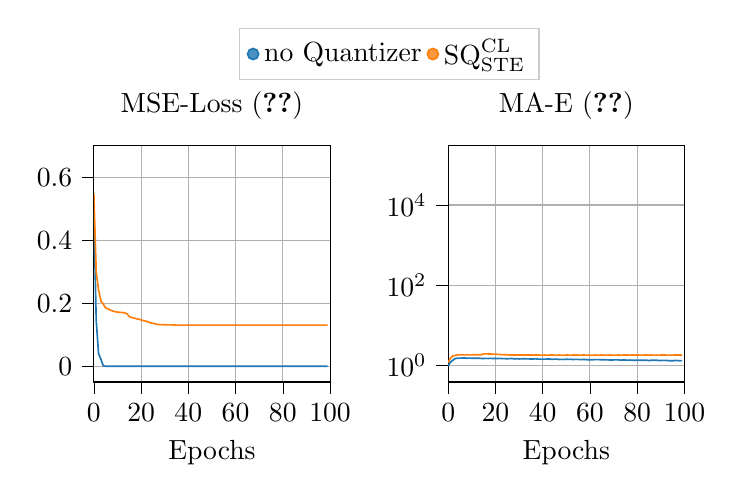
\begin{tikzpicture}

\definecolor{darkgray176}{RGB}{176,176,176}
\definecolor{darkorange25512714}{RGB}{255,127,14}
\definecolor{lightgray204}{RGB}{204,204,204}
\definecolor{steelblue31119180}{RGB}{31,119,180}

\begin{axis}[
name = plot1,
    width=3cm,  % Adjust the width of the plot
    height=3cm,  % Adjust the height of the plot
    scale only axis, 
    xlabel={Epochs},
legend cell align={center},
legend style={
  fill opacity=0.8,
  draw opacity=1,
  text opacity=1,
  at={(1.25,1.5)},
  anchor=north,
  draw=lightgray204,
  legend columns = -1
  mark=*
},
legend image code/.code={
        \draw[mark options={scale=1}, mark=*] plot coordinates {(0.3cm,0cm)}; % Use points in the legend
    },
tick align=outside,
tick pos=left,
x grid style={darkgray176},
xmajorgrids,
xmin=0, xmax=100,
xtick style={color=black},
y grid style={darkgray176},
ylabel={},
title={MSE-Loss (\ref{equ:MSELoss})},
ymajorgrids,
ymin=-0.05, 
ymax=0.7,
ytick style={color=black},
]
\addplot [semithick, steelblue31119180]
table {%
0 0.491439277626574
1 0.145839979875833
2 0.040147550188005
3 0.0221479450738989
4 0.00149579956594971
5 0.000185314791179735
6 2.88211019144455e-05
7 9.26099238910183e-06
8 5.63369642819112e-06
9 4.19628487658485e-06
10 3.45550454594701e-06
11 3.07767361245226e-06
12 2.69274032850575e-06
13 2.5199281473185e-06
14 2.32981874470539e-06
15 2.34445380689152e-06
16 2.23870044637131e-06
17 2.18607506899549e-06
18 2.14165844633563e-06
19 2.14033544194869e-06
20 2.19737296721045e-06
21 1.99292602428924e-06
22 2.05227904789707e-06
23 2.06425206110727e-06
24 2.0497238110101e-06
25 2.09024653652873e-06
26 1.96800227211469e-06
27 1.98377456345733e-06
28 2.04983100771627e-06
29 1.93138959105754e-06
30 1.97143960096093e-06
31 1.96656108060764e-06
32 1.96128012035343e-06
33 1.87406848142269e-06
34 1.95899548123064e-06
35 2.06950092014527e-06
36 1.77598596714649e-06
37 1.89258909054116e-06
38 1.86770988570095e-06
39 1.90023664551175e-06
40 1.98853274846311e-06
41 1.73420043834979e-06
42 1.83053138744999e-06
43 1.83887237433022e-06
44 1.84024018024732e-06
45 1.90997533066628e-06
46 1.73806030858443e-06
47 1.80118299307216e-06
48 1.77944000292866e-06
49 1.76767705089595e-06
50 1.78103714961068e-06
51 1.75996178718733e-06
52 1.79876262444878e-06
53 1.68875101220228e-06
54 1.72277751419593e-06
55 1.74380437144303e-06
56 1.65202610490772e-06
57 1.76343048156535e-06
58 1.62815765590901e-06
59 1.71006245526205e-06
60 1.67780812488743e-06
61 1.72043847649969e-06
62 1.65427349096531e-06
63 1.60840335319814e-06
64 1.6785292990398e-06
65 1.62734447482625e-06
66 1.66653455679233e-06
67 1.55285236923791e-06
68 1.59857226366006e-06
69 1.5729478062908e-06
70 1.58914339040814e-06
71 1.55204935845105e-06
72 1.56630324249829e-06
73 1.57998718153763e-06
74 1.52933544721759e-06
75 1.59393987128011e-06
76 1.61161236163954e-06
77 1.4681082392279e-06
78 1.52794630263894e-06
79 1.49592511971763e-06
80 1.48590521772443e-06
81 1.55174371780464e-06
82 1.41478302101003e-06
83 1.49139737778946e-06
84 1.48048299807561e-06
85 1.51897484758891e-06
86 1.38714931934843e-06
87 1.49776836886953e-06
88 1.41997981466642e-06
89 1.47431763927672e-06
90 1.42272246303093e-06
91 1.4149008913151e-06
92 1.39491322596242e-06
93 1.43892097185226e-06
94 1.3585801499705e-06
95 1.36681164034219e-06
96 1.38891166662127e-06
97 1.37259174018019e-06
98 1.36007890725973e-06
99 1.33940678363167e-06
};
\addlegendentry{no Quantizer}
\addplot [semithick, darkorange25512714]
table {%
0 0.549000259801745
1 0.299871038094163
2 0.242189251571894
3 0.207308624267578
4 0.197074625216424
5 0.185634178325534
6 0.182380964674056
7 0.178326630882919
8 0.175201226659119
9 0.173283803023398
10 0.172094418533146
11 0.171343371406198
12 0.170765378408134
13 0.169521951183677
14 0.167103111922741
15 0.157875367105007
16 0.154614733763039
17 0.153081586278975
18 0.150951494216919
19 0.149476350657642
20 0.147199265860021
21 0.144910294152796
22 0.143213532932103
23 0.14128946762532
24 0.137701354525983
25 0.136567906014621
26 0.134132204532623
27 0.132960757054389
28 0.132355139888823
29 0.131965770825744
30 0.131745044507086
31 0.131587471209466
32 0.13147689602524
33 0.131349040202796
34 0.131103035457432
35 0.130517799466848
36 0.130464115925133
37 0.130513427942991
38 0.130506151787937
39 0.130541185207665
40 0.130534353867173
41 0.130492865376174
42 0.130522380650043
43 0.130526529125869
44 0.130550112396479
45 0.130531256340444
46 0.130503811851144
47 0.130515778191388
48 0.130510073944926
49 0.130536538757384
50 0.130526625037193
51 0.130501929484308
52 0.130520934864879
53 0.130509537316859
54 0.130512963078916
55 0.130522072032094
56 0.130513535268605
57 0.130511100739241
58 0.130539780512452
59 0.130513597756624
60 0.130501266375184
61 0.130528594397008
62 0.130528959475458
63 0.130543941237032
64 0.130528621524572
65 0.130521844916046
66 0.130523137196898
67 0.130502953402698
68 0.130502688154578
69 0.130511386707425
70 0.130524727001786
71 0.130521879352629
72 0.130487557888031
73 0.130523864358664
74 0.130489279292524
75 0.130496246568859
76 0.130508339770138
77 0.130523177161813
78 0.130494157969952
79 0.130501418083906
80 0.130529735192657
81 0.130518131420016
82 0.130508684828877
83 0.130500476054847
84 0.130506072625518
85 0.130520362116396
86 0.13052210765332
87 0.130500621564686
88 0.130523995541036
89 0.130495601221919
90 0.130508861780167
91 0.130531919181347
92 0.130510828539729
93 0.130509101711214
94 0.130512753784657
95 0.130492839120328
96 0.130500469848514
97 0.130490967720747
98 0.130495262987912
99 0.130493671834469
};
\addlegendentry{$\text{SQ}^{\text{CL}}_\text{STE}$ }
\end{axis}



\begin{axis}[
        at={(plot1.east)}, % Align it next to the first plot
    anchor=west,
    width=3cm,  % Adjust the width of the plot
    height=3cm,  % Adjust 
     xshift=1.5cm, %the height of the plot
    scale only axis, 
    title={MA-E (\ref{equ:MAE})},
log basis y={10},
tick align=outside,
tick pos=left,
x grid style={darkgray176},
xlabel={Epochs},
xmajorgrids,
xmin=0, xmax=100,
xtick style={color=black},
y grid style={darkgray176},
ymajorgrids,
ymin=0.37772735089694, ymax=302220.574977491,
ymode=log,
ytick style={color=black}
]
\addplot [semithick, steelblue31119180]
table {%
0 0.967797929048538
1 1.18999158143997
2 1.3280640522639
3 1.45739589532216
4 1.48696814775467
5 1.49455015858014
6 1.4984413087368
7 1.50753791928291
8 1.48351823091507
9 1.49526984492938
10 1.48783353964488
11 1.47498019933701
12 1.48275196949641
13 1.48674787680308
14 1.46704434951146
15 1.4647004087766
16 1.47203040917714
17 1.46624130010605
18 1.47390285730362
19 1.46274871031443
20 1.45827481945356
21 1.4549953798453
22 1.47385632594426
23 1.45014885862668
24 1.4484273036321
25 1.44306247830391
26 1.45101089477539
27 1.46076002319654
28 1.4252666870753
29 1.44686559240023
30 1.42446284294128
31 1.43271813591321
32 1.44545921683311
33 1.43073971271515
34 1.43180764913559
35 1.4184127052625
36 1.42323799530665
37 1.43259494105975
38 1.41359353661537
39 1.40981947978338
40 1.40724654197693
41 1.406930210193
42 1.41545903881391
43 1.41366568605105
44 1.3914620300134
45 1.41088707844416
46 1.41070099075635
47 1.38227074742317
48 1.38994129101435
49 1.38415230512619
50 1.40318608283997
51 1.39011055628459
52 1.39560886224111
53 1.38020410339038
54 1.39084505240122
55 1.38685316840808
56 1.36806154648463
57 1.38207839330037
58 1.3816189746062
59 1.35772135059039
60 1.35888500610987
61 1.36058977842331
62 1.37051539222399
63 1.36771312554677
64 1.36801095207532
65 1.35492933392525
66 1.36689975063006
67 1.35233320991198
68 1.34628750681877
69 1.34210849801699
70 1.34686796466509
71 1.35329723159472
72 1.3503042280674
73 1.33104382157326
74 1.34038360118866
75 1.33892426292102
76 1.324663601319
77 1.33607966899872
78 1.32023986379306
79 1.31750364899635
80 1.32620007594426
81 1.31737558444341
82 1.31540066798528
83 1.32045937975248
84 1.32427805860837
85 1.29337703386943
86 1.32230117917061
87 1.32707501451174
88 1.32695627212524
89 1.30781185030937
90 1.30090575218201
91 1.31222044229507
92 1.3084713101387
93 1.3018348634243
94 1.2810719927152
95 1.27780377070109
96 1.30311262607574
97 1.29654068748156
98 1.288038311402
99 1.29606095949809
};
\addplot [semithick, darkorange25512714]
table {%
0 1.15177705486616
1 1.49898407856623
2 1.68984109958013
3 1.74100794792175
4 1.81043399969737
5 1.80887944698334
6 1.81068992614746
7 1.80273396571477
8 1.79722727139791
9 1.80120892524719
10 1.79876539707184
11 1.8107432325681
12 1.81065675814947
13 1.82434448401133
14 1.8075327595075
15 1.9066148519516
16 1.90987679560979
17 1.90051119724909
18 1.88925451437632
19 1.88267554442088
20 1.87240897019704
21 1.85495265722275
22 1.84392866690954
23 1.8233410914739
24 1.80795597235362
25 1.81095338265101
26 1.7882888674736
27 1.79436893860499
28 1.7830516854922
29 1.78319657246272
30 1.78521246512731
31 1.78399416208267
32 1.77897806962331
33 1.78484630187352
34 1.78965667883555
35 1.78724503119787
36 1.77722928126653
37 1.78671556711197
38 1.78292543490728
39 1.77811615069707
40 1.77549083630244
41 1.78069831530253
42 1.77355553309123
43 1.77956559658051
44 1.78367565870285
45 1.77791599432627
46 1.77011037667592
47 1.7834709127744
48 1.77421322266261
49 1.77529484033585
50 1.78160897095998
51 1.77904099623362
52 1.77556119362513
53 1.78328501383464
54 1.78391941785812
55 1.78135044972102
56 1.7737685362498
57 1.78358612060547
58 1.77882724603017
59 1.7719974120458
60 1.77522218624751
61 1.77480307420095
62 1.77991149822871
63 1.77920944690704
64 1.77348047494888
65 1.78633494377136
66 1.77663913567861
67 1.77468335231145
68 1.78009341160456
69 1.78007904291153
70 1.77263360420863
71 1.77128464778264
72 1.7840326944987
73 1.77595264911652
74 1.77936276594798
75 1.78149652481079
76 1.78397656679153
77 1.77532234191895
78 1.78522520860036
79 1.77818075418472
80 1.78747274080912
81 1.77702915668488
82 1.77857061624527
83 1.77995453675588
84 1.7965615272522
85 1.77666591008504
86 1.78238356908162
87 1.77309301694234
88 1.78007437785467
89 1.77789382537206
90 1.78000446160634
91 1.78402543465296
92 1.78007783095042
93 1.77365928490957
94 1.78022813002268
95 1.77402989466985
96 1.78552823464076
97 1.77882620096207
98 1.78523919582367
99 1.7766180674235
};
\end{axis}
\end{tikzpicture}

    \caption{Training \gls{MSE} and \gls{MA-E} when using a no quantizer and the standard training using the \gls{STE} with \gls{CL}.}
    \label{fig:enter-label}
\end{figure}
\begin{figure}[t]
    \centering
    % This file was created with tikzplotlib v0.10.1.
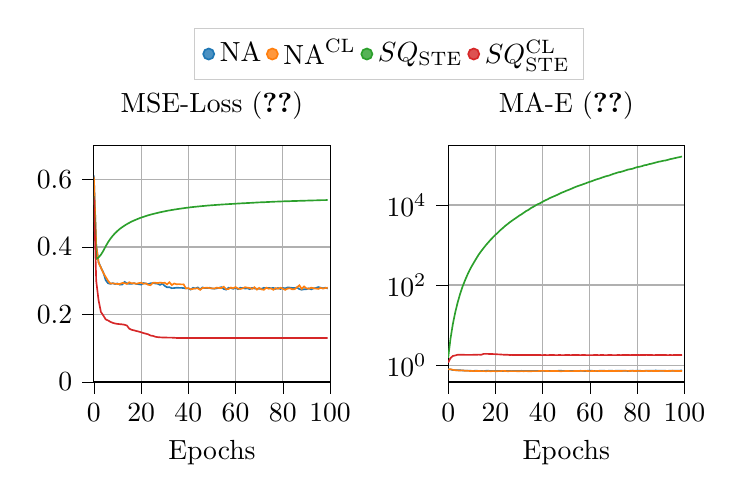
\begin{tikzpicture}

\definecolor{crimson2143940}{RGB}{214,39,40}
\definecolor{darkgray176}{RGB}{176,176,176}
\definecolor{darkorange25512714}{RGB}{255,127,14}
\definecolor{forestgreen4416044}{RGB}{44,160,44}
\definecolor{lightgray204}{RGB}{204,204,204}
\definecolor{steelblue31119180}{RGB}{31,119,180}

\begin{axis}[
name = plot1,
    width=3cm,  % Adjust the width of the plot
    height=3cm,  % Adjust the height of the plot
    scale only axis, 
    xlabel={Epochs},
legend cell align={center},
legend style={
  fill opacity=0.8,
  draw opacity=1,
  text opacity=1,
  at={(1.25,1.5)},
  anchor=north,
  draw=lightgray204,
  legend columns = -1
  mark=*
},
legend image code/.code={
        \draw[mark options={scale=1}, mark=*] plot coordinates {(0.3cm,0cm)}; % Use points in the legend
    },
tick align=outside,
tick pos=left,
x grid style={darkgray176},
xmajorgrids,
xmin=0, xmax=100,
xtick style={color=black},
y grid style={darkgray176},
ylabel={},
title={MSE-Loss (\ref{equ:MSELoss})},
ymajorgrids,
ymin=0, 
ymax=0.7,
ytick style={color=black},
]
\addplot [semithick, steelblue31119180]
table {%
0 0.611941409394145
1 0.404460925444961
2 0.355163639776409
3 0.339247392460704
4 0.324812070466578
5 0.301795873902738
6 0.292822175815701
7 0.290735897243023
8 0.292805431999266
9 0.290305355966091
10 0.291941600158811
11 0.288333343707025
12 0.288737422563136
13 0.296677809603512
14 0.292281404785812
15 0.290858758054674
16 0.290767313160002
17 0.292714920699596
18 0.290587794758379
19 0.289766863293946
20 0.288406750351191
21 0.293193183898926
22 0.291701209932566
23 0.290007071204483
24 0.292503394111991
25 0.293332264944911
26 0.291972432099283
27 0.291046844929457
28 0.287716829553247
29 0.291602838911116
30 0.284840544752777
31 0.280512229338288
32 0.280809077531099
33 0.277989823311567
34 0.278361989110708
35 0.279393471904099
36 0.279003665581346
37 0.279020595915616
38 0.278237650796771
39 0.277349738404155
40 0.277278342619538
41 0.273919279158115
42 0.279123209051788
43 0.27709675514698
44 0.28020255998522
45 0.27470947098732
46 0.280286003962159
47 0.27813413977623
48 0.278169064290822
49 0.279392674587667
50 0.277171799391508
51 0.276486691772938
52 0.277413161180913
53 0.279150147378445
54 0.281031813181937
55 0.275608771234751
56 0.27366885086149
57 0.279172012083232
58 0.278515524618328
59 0.276100231125951
60 0.278760932698846
61 0.275043711975217
62 0.279179656289518
63 0.278528353877366
64 0.276965564243495
65 0.277563843168318
66 0.275165799811482
67 0.2789791867733
68 0.276749472655356
69 0.276790994957089
70 0.276459479801357
71 0.276327098228037
72 0.279078826345503
73 0.27826146197319
74 0.278874768920243
75 0.277815463848412
76 0.278804229311645
77 0.275874389119446
78 0.278570503793657
79 0.275502957567573
80 0.278709277048707
81 0.277353476390243
82 0.280052238218486
83 0.279736127734184
84 0.278723088487983
85 0.278621223472059
86 0.279907686054707
87 0.275282921276987
88 0.273415324039757
89 0.274746660880744
90 0.274893422745168
91 0.277455612197518
92 0.274458181723952
93 0.277263621002436
94 0.278553314588964
95 0.281348010055721
96 0.279461028672755
97 0.277654385901988
98 0.279517267264426
99 0.276829372189939
};
\addlegendentry{NA}
\addplot [semithick, darkorange25512714]
table {%
0 0.608796063810587
1 0.404834068283439
2 0.353451243817806
3 0.338568493880332
4 0.323459391139448
5 0.311533840574324
6 0.300045564420521
7 0.291719058051705
8 0.292339117482305
9 0.291288265392184
10 0.290410711705685
11 0.290524671278894
12 0.293199801497161
13 0.293025554820895
14 0.290531463526189
15 0.295489782825112
16 0.292294562637806
17 0.292943701155484
18 0.290817392267287
19 0.293005076251924
20 0.294164174884558
21 0.291099690787494
22 0.292309767723083
23 0.288032758355141
24 0.286823302768171
25 0.293853967666626
26 0.294363110654056
27 0.292947210237384
28 0.294658658236265
29 0.293523136638105
30 0.293943503648043
31 0.289424084164202
32 0.295608305335045
33 0.287112329237163
34 0.291889309346676
35 0.289596081763506
36 0.290031305097044
37 0.289163750000298
38 0.289397771321237
39 0.277202979832888
40 0.278286978907883
41 0.274547535397112
42 0.275911723800004
43 0.277363488964736
44 0.277568548239768
45 0.273078170023859
46 0.278599904976785
47 0.278825132340193
48 0.279550102636218
49 0.278170816399157
50 0.277482765451074
51 0.276931995548308
52 0.27972166389972
53 0.278546011075377
54 0.278506645992398
55 0.282398849375546
56 0.275060715161264
57 0.275370138250291
58 0.279895563319325
59 0.277708165705204
60 0.281192395374179
61 0.27682488746196
62 0.275595603443682
63 0.277571296684444
64 0.280766646973789
65 0.27943359337002
66 0.278589633107185
67 0.275965581551194
68 0.280830531902611
69 0.273645771220326
70 0.278702991873026
71 0.274352182485163
72 0.273271102510393
73 0.27945484072715
74 0.276404253445566
75 0.277227476261556
76 0.273234584100544
77 0.278205651275814
78 0.276227233588696
79 0.279279652908444
80 0.276720661975443
81 0.273039626404643
82 0.276899457156658
83 0.277564294412732
84 0.274600497633219
85 0.27512222328037
86 0.280471811644733
87 0.286434203542769
88 0.275768381729722
89 0.283131299182773
90 0.277525585323572
91 0.276315912701189
92 0.279433982238174
93 0.277927031427622
94 0.276872227557004
95 0.275729609794915
96 0.278945564739406
97 0.276855052880943
98 0.278311800837517
99 0.279406821645796
};
\addlegendentry{$\text{NA}^\text{CL}$}
\addplot [semithick, forestgreen4416044]
table {%
0 0.55088772341609
1 0.364599603518844
2 0.368866781711578
3 0.377288254261017
4 0.388566744953394
5 0.401835393205285
6 0.414005573749542
7 0.424335187733173
8 0.433307941555977
9 0.440919484496117
10 0.447635944843292
11 0.453682038679719
12 0.458860293194652
13 0.463521628290415
14 0.467869847580791
15 0.471703230798244
16 0.475401790723205
17 0.478585365355015
18 0.481512870833278
19 0.484425481408834
20 0.487144548967481
21 0.489412767782807
22 0.491777189701796
23 0.493936263769865
24 0.495904034361243
25 0.497762332350016
26 0.499550337582827
27 0.501130907699466
28 0.502885586768389
29 0.504318796187639
30 0.505741798982024
31 0.507270608186722
32 0.508436697110534
33 0.509720933899283
34 0.510865337014198
35 0.511979941368103
36 0.513019118696451
37 0.513959438443184
38 0.514955953866243
39 0.516012669444084
40 0.516867266148329
41 0.517744843870401
42 0.51857935076952
43 0.519320396065712
44 0.519961907505989
45 0.520658597141504
46 0.521395146280527
47 0.521903126507998
48 0.522700056582689
49 0.52323027163744
50 0.523826842874289
51 0.524266020983458
52 0.524801029682159
53 0.525233933061361
54 0.525834440082312
55 0.526259167104959
56 0.526617806315422
57 0.527145440518856
58 0.527537268251181
59 0.527885058254004
60 0.528327745348215
61 0.52878401529789
62 0.529222670078278
63 0.529591565400362
64 0.529899104863405
65 0.530336342602968
66 0.530688235938549
67 0.530990009218454
68 0.531487732738256
69 0.531842892467976
70 0.532275775909424
71 0.532542983800173
72 0.532737836956978
73 0.533120610415936
74 0.533493458986282
75 0.533814318478107
76 0.534058399617672
77 0.534519419878721
78 0.534666323184967
79 0.534989660829306
80 0.535261952996254
81 0.535537146002054
82 0.535684410214424
83 0.535837888389826
84 0.536177230507135
85 0.53638651779294
86 0.536517620921135
87 0.536831999242306
88 0.536970202863216
89 0.537155061453581
90 0.537432105869055
91 0.53773717880249
92 0.53779073548317
93 0.538084347188473
94 0.538191051691771
95 0.53855269575119
96 0.53880144482851
97 0.538929655462503
98 0.5389938133955
99 0.539319223552942
};
\addlegendentry{$SQ_\text{STE}$}
\addplot [semithick, crimson2143940]
table {%
0 0.549000259801745
1 0.299871038094163
2 0.242189251571894
3 0.207308624267578
4 0.197074625216424
5 0.185634178325534
6 0.182380964674056
7 0.178326630882919
8 0.175201226659119
9 0.173283803023398
10 0.172094418533146
11 0.171343371406198
12 0.170765378408134
13 0.169521951183677
14 0.167103111922741
15 0.157875367105007
16 0.154614733763039
17 0.153081586278975
18 0.150951494216919
19 0.149476350657642
20 0.147199265860021
21 0.144910294152796
22 0.143213532932103
23 0.14128946762532
24 0.137701354525983
25 0.136567906014621
26 0.134132204532623
27 0.132960757054389
28 0.132355139888823
29 0.131965770825744
30 0.131745044507086
31 0.131587471209466
32 0.13147689602524
33 0.131349040202796
34 0.131103035457432
35 0.130517799466848
36 0.130464115925133
37 0.130513427942991
38 0.130506151787937
39 0.130541185207665
40 0.130534353867173
41 0.130492865376174
42 0.130522380650043
43 0.130526529125869
44 0.130550112396479
45 0.130531256340444
46 0.130503811851144
47 0.130515778191388
48 0.130510073944926
49 0.130536538757384
50 0.130526625037193
51 0.130501929484308
52 0.130520934864879
53 0.130509537316859
54 0.130512963078916
55 0.130522072032094
56 0.130513535268605
57 0.130511100739241
58 0.130539780512452
59 0.130513597756624
60 0.130501266375184
61 0.130528594397008
62 0.130528959475458
63 0.130543941237032
64 0.130528621524572
65 0.130521844916046
66 0.130523137196898
67 0.130502953402698
68 0.130502688154578
69 0.130511386707425
70 0.130524727001786
71 0.130521879352629
72 0.130487557888031
73 0.130523864358664
74 0.130489279292524
75 0.130496246568859
76 0.130508339770138
77 0.130523177161813
78 0.130494157969952
79 0.130501418083906
80 0.130529735192657
81 0.130518131420016
82 0.130508684828877
83 0.130500476054847
84 0.130506072625518
85 0.130520362116396
86 0.13052210765332
87 0.130500621564686
88 0.130523995541036
89 0.130495601221919
90 0.130508861780167
91 0.130531919181347
92 0.130510828539729
93 0.130509101711214
94 0.130512753784657
95 0.130492839120328
96 0.130500469848514
97 0.130490967720747
98 0.130495262987912
99 0.130493671834469
};
\addlegendentry{$SQ_\text{STE}^\text{CL}$}
\end{axis}

\begin{axis}[
        at={(plot1.east)}, % Align it next to the first plot
    anchor=west,
    width=3cm,  % Adjust the width of the plot
    height=3cm,  % Adjust 
     xshift=1.5cm, %the height of the plot
    scale only axis, 
    title={MA-E (\ref{equ:MAE})},
log basis y={10},
tick align=outside,
tick pos=left,
x grid style={darkgray176},
xlabel={Epochs},
xmajorgrids,
xmin=0, xmax=100,
xtick style={color=black},
y grid style={darkgray176},
ymajorgrids,
ymin=0.37772735089694, ymax=302220.574977491,
ymode=log,
ytick style={color=black}
]
\addplot [semithick, steelblue31119180]
table {%
0 0.784316565593084
1 0.781134277582169
2 0.75108015537262
3 0.747364002466202
4 0.740072242418925
5 0.742147266864777
6 0.734453016519547
7 0.725739912192027
8 0.725482821464539
9 0.725872256358465
10 0.71623806754748
11 0.717047673463821
12 0.724361884593964
13 0.710147565603256
14 0.71484912832578
15 0.710747335354487
16 0.718673286835353
17 0.720987143119176
18 0.712739396095276
19 0.71228361527125
20 0.712281819184621
21 0.708043175935745
22 0.713457111517588
23 0.707725787162781
24 0.710828079779943
25 0.710757700602214
26 0.708714254697164
27 0.707544475793839
28 0.710333482424418
29 0.71262610356013
30 0.712401813268661
31 0.718252156178157
32 0.716661332050959
33 0.71257671713829
34 0.714103603363037
35 0.715125119686127
36 0.717597754796346
37 0.71170742114385
38 0.715586141745249
39 0.713813449939092
40 0.716613757610321
41 0.713593037923177
42 0.712899752457937
43 0.716273045539856
44 0.716301995515823
45 0.71634173989296
46 0.715151470899582
47 0.720994468530019
48 0.719423288106918
49 0.709180527925491
50 0.714239386717478
51 0.714714256922404
52 0.716577911376953
53 0.715655094385147
54 0.718004085620244
55 0.715379571914673
56 0.718934539953868
57 0.715375073750814
58 0.7126762231191
59 0.718821219603221
60 0.718017041683197
61 0.718857727448146
62 0.714162311951319
63 0.712864913543065
64 0.719291679064433
65 0.722002234061559
66 0.721423623959223
67 0.712879719336828
68 0.719574244817098
69 0.722789339224498
70 0.716404211521149
71 0.719432612260183
72 0.722413490215937
73 0.71859184106191
74 0.722885553042094
75 0.721519402662913
76 0.712608919541041
77 0.720148783922195
78 0.72747211654981
79 0.716309491793315
80 0.723044633865356
81 0.720361840724945
82 0.716077470779419
83 0.715186387300491
84 0.727467252810796
85 0.722101583083471
86 0.71787742972374
87 0.724995827674866
88 0.730283008019129
89 0.718816594282786
90 0.718360368410746
91 0.722093685468038
92 0.71898397008578
93 0.715825537840525
94 0.726787326733271
95 0.721089694897334
96 0.722597585121791
97 0.723732564846675
98 0.724596387147903
99 0.73590941230456
};
\addplot [semithick, darkorange25512714]
table {%
0 0.780062007904053
1 0.785003300507863
2 0.760595844189326
3 0.743645322322845
4 0.738197988271713
5 0.727404369910558
6 0.73832106590271
7 0.720802754163742
8 0.72067355910937
9 0.713183629512787
10 0.71515442331632
11 0.705765650669734
12 0.712433300415675
13 0.712155882517497
14 0.704875973860423
15 0.708641225099564
16 0.70104883313179
17 0.708326105276744
18 0.701419488588969
19 0.70841281414032
20 0.702454942464829
21 0.704174659649531
22 0.704577163855235
23 0.717927555243174
24 0.71203598578771
25 0.70237233042717
26 0.705128888289134
27 0.707403345902761
28 0.706829740603765
29 0.703698541720708
30 0.700653398036957
31 0.706547838449478
32 0.703005766868591
33 0.707197372118632
34 0.701774646838506
35 0.702649648984273
36 0.705712916453679
37 0.705201524496079
38 0.706422601143519
39 0.714035723606745
40 0.718191597859065
41 0.714887227614721
42 0.710324345032374
43 0.705266364415487
44 0.713340729475021
45 0.710121959447861
46 0.713599592447281
47 0.704361832141876
48 0.703318081299464
49 0.707208555936813
50 0.708930063247681
51 0.708541176716487
52 0.706024523576101
53 0.706982847054799
54 0.713527637720108
55 0.712104618549347
56 0.715284230311712
57 0.714014929533005
58 0.718396516640981
59 0.712120225032171
60 0.70300657749176
61 0.712330993016561
62 0.705399974187215
63 0.716652369499207
64 0.711654380957286
65 0.715257356564204
66 0.709045793612798
67 0.710406134525935
68 0.713286699851354
69 0.713970551888148
70 0.714134921630224
71 0.708393577734629
72 0.71591382821401
73 0.708847548564275
74 0.716458161671956
75 0.717960963646571
76 0.716552470127741
77 0.71113104224205
78 0.718919990460078
79 0.707574218511581
80 0.714642171065013
81 0.714416901270548
82 0.706916064023972
83 0.711730722586314
84 0.718201941251755
85 0.708433689673742
86 0.716953217983246
87 0.710274974505107
88 0.712638219197591
89 0.712405643860499
90 0.717525462309519
91 0.716002144416173
92 0.711754639943441
93 0.713744324445724
94 0.711945599317551
95 0.720099818706512
96 0.712131476402283
97 0.712278308471044
98 0.713869651158651
99 0.712531715631485
};
\addplot [semithick, forestgreen4416044]
table {%
0 1.52191224098206
1 4.62942314147949
2 10.7700797080994
3 20.8528925577799
4 36.3747828801473
5 58.6029336293538
6 88.5621025085449
7 125.331676737467
8 172.717534383138
9 231.091755167643
10 297.690074666341
11 374.748385620117
12 470.715333048503
13 584.981895955404
14 705.257332356771
15 840.939318847656
16 996.562082926432
17 1164.62107543945
18 1361.14012451172
19 1563.32934977214
20 1795.80465087891
21 2030.06355794271
22 2333.39939778646
23 2611.14085286458
24 2954.9336710612
25 3288.2523844401
26 3671.10323079427
27 4043.10830891927
28 4452.31261393229
29 4877.00172526042
30 5379.12698567708
31 5833.47943522135
32 6415.72179361979
33 7065.05356445312
34 7571.12750651042
35 8357.25302734375
36 8967.70460611979
37 9765.99383138021
38 10491.2435546875
39 11156.7108072917
40 12068.3065917969
41 12973.3904459635
42 13800.2222981771
43 14856.6091145833
44 15786.3408854167
45 16714.0112630208
46 17757.7693684896
47 18953.1794596354
48 20258.6350585938
49 21322.02734375
50 22663.4591471354
51 23886.9681640625
52 25237.6015299479
53 26856.3376953125
54 28415.2879557292
55 29912.9180338542
56 31284.2891276042
57 32826.7267578125
58 34398.5539713542
59 36384.1580729167
60 38069.0947265625
61 39918.037890625
62 42019.1438151042
63 44091.3958984375
64 45745.9811848958
65 48158.7407552083
66 50503.2204427083
67 52731.0869791667
68 54221.2240885417
69 57230.4666666667
70 60084.062109375
71 62508.45625
72 65623.8298177083
73 66958.82265625
74 69791.838671875
75 72859.9966145833
76 76534.0283854167
77 78393.4149739583
78 80455.669921875
79 84537.4856770833
80 88595.2701822917
81 90587.526953125
82 93212.7028645833
83 98404.0579427083
84 100310.597395833
85 104992.432682292
86 107600.389583333
87 111554.88125
88 115896.441666667
89 120097.72578125
90 123141.6984375
91 127448.078385417
92 129743.982552083
93 134410.966927083
94 140104.898958333
95 143944.02421875
96 148692.367708333
97 153510.48828125
98 157471.023958333
99 162929.313541667
};
\addplot [semithick, crimson2143940]
table {%
0 1.15177705486616
1 1.49898407856623
2 1.68984109958013
3 1.74100794792175
4 1.81043399969737
5 1.80887944698334
6 1.81068992614746
7 1.80273396571477
8 1.79722727139791
9 1.80120892524719
10 1.79876539707184
11 1.8107432325681
12 1.81065675814947
13 1.82434448401133
14 1.8075327595075
15 1.9066148519516
16 1.90987679560979
17 1.90051119724909
18 1.88925451437632
19 1.88267554442088
20 1.87240897019704
21 1.85495265722275
22 1.84392866690954
23 1.8233410914739
24 1.80795597235362
25 1.81095338265101
26 1.7882888674736
27 1.79436893860499
28 1.7830516854922
29 1.78319657246272
30 1.78521246512731
31 1.78399416208267
32 1.77897806962331
33 1.78484630187352
34 1.78965667883555
35 1.78724503119787
36 1.77722928126653
37 1.78671556711197
38 1.78292543490728
39 1.77811615069707
40 1.77549083630244
41 1.78069831530253
42 1.77355553309123
43 1.77956559658051
44 1.78367565870285
45 1.77791599432627
46 1.77011037667592
47 1.7834709127744
48 1.77421322266261
49 1.77529484033585
50 1.78160897095998
51 1.77904099623362
52 1.77556119362513
53 1.78328501383464
54 1.78391941785812
55 1.78135044972102
56 1.7737685362498
57 1.78358612060547
58 1.77882724603017
59 1.7719974120458
60 1.77522218624751
61 1.77480307420095
62 1.77991149822871
63 1.77920944690704
64 1.77348047494888
65 1.78633494377136
66 1.77663913567861
67 1.77468335231145
68 1.78009341160456
69 1.78007904291153
70 1.77263360420863
71 1.77128464778264
72 1.7840326944987
73 1.77595264911652
74 1.77936276594798
75 1.78149652481079
76 1.78397656679153
77 1.77532234191895
78 1.78522520860036
79 1.77818075418472
80 1.78747274080912
81 1.77702915668488
82 1.77857061624527
83 1.77995453675588
84 1.7965615272522
85 1.77666591008504
86 1.78238356908162
87 1.77309301694234
88 1.78007437785467
89 1.77789382537206
90 1.78000446160634
91 1.78402543465296
92 1.78007783095042
93 1.77365928490957
94 1.78022813002268
95 1.77402989466985
96 1.78552823464076
97 1.77882620096207
98 1.78523919582367
99 1.7766180674235
};

\end{axis}

\end{tikzpicture}


    \caption{Training \gls{MSE} and \gls{MA-E} when using \gls{NA} or the \gls{STE} for training with and without \gls{CL}. Note that the \gls{MA-E} curves of NA and $\text{NA}^\text{CL}$ are overlapping.}
    \label{fig:NIvsSTE}
\end{figure}


In evaluating the proposed framework, we focus on fundamental properties of neural codecs. We note that further investigations not part of the article can easily and quickly be accomplished with the proposed method. From our point of view, these are but are not limited to: (1) Network layers, activations, or regularizers directly before or after the quantizer (e.g., dropout leads to correlated features such that a \gls{VQ} might work better than a \gls{SQ}), (2) Other gradient estimators like ReinMax \cite{liu2024bridging}, or SPIGOT \cite{peng2018backpropagating}, (3) different quantizers and bitrates including soft quantizers \cite{agustsson2017soft,Jang2017,maddison2017gumbel}.

A comparison of training time and required GPU memory is given in Table~\ref{tab:mem_time}. The proposed system takes less than an hour to train and requires less than $400$~MB of GPU memory. Consequently, multiple systems can be tested in parallel, enabling rapid prototyping. Compared to full-scale neural codecs like \gls{DAC}, temporal and hardware requirements are significantly reduced, leading to a significantly reduced cost.


\subsection{Experiments with the Proposed Evaluation Framework}

\textbf{No Quantizer vs. STE}: First, in Figure~\ref{fig:enter-label}, we compare the training of the proposed system without a quantizer and with $\text{SQ}_\text{STE}^\text{CL}$. As expected, the loss without quantizer approaches zero very quickly. For $\text{SQ}_\text{STE}^\text{CL}$, the model is able to reduce the loss; however, it converges to an \gls{MSE} of $\approx 0.13$. Theoretically, when $\mathcal{Q}$ has the same number of bits or more than the input, perfect reconstruction is possible. For $\text{SQ}_\text{STE}^\text{CL}$, both an input frame and the bits of the quantizer are the same (60~Bits). When doubling the bits in the quantizer to 120, the \gls{MSE} loss yields comparable results to a quantizer-free system.  The \gls{MA-E} in Figure~\ref{fig:enter-label} is stable for all models, as it converges to a fixed value over the epochs. A stable, non-diverging system is important. Otherwise, the input of the decoder constantly changes, and the model cannot learn.

\textbf{no CL vs. CL}: In Figure~\ref{fig:NIvsSTE} we compare \gls{NA} vs. \gls{STE} with and without \gls{CL}. The \gls{MSE} and \gls{MA-E} values of NA and $\text{NA}^\text{CL}$ are comparable over training, showing that \gls{CL} has no effect on them. For $\text{SQ}_\text{STE}^\text{CL}$ and $\text{SQ}_\text{STE}$ the \gls{MSE} and \gls{MA-E} show a strong difference. Without \gls{CL}, the encoder output $E$ grows unboundedly over training, whereas when using \gls{CL}, the \gls{MA-E} converges. In \cite{VanDenOord2017}, the authors mention the same behavior for training a neural codec using the \gls{STE} without \gls{CL}. The growing $E$ translates to a diverging loss for $\text{SQ}_\text{STE}$. The different effect of  \gls{CL} on \gls{NA} and \gls{STE} is remarkable. In the following, we analyze what incentivises the encoder to produce larger and larger $E$ for \gls{STE} without \gls{CL} but not for \gls{NA}. 



\begin{figure}[t]
    \centering
    % This file was created with tikzplotlib v0.10.1.
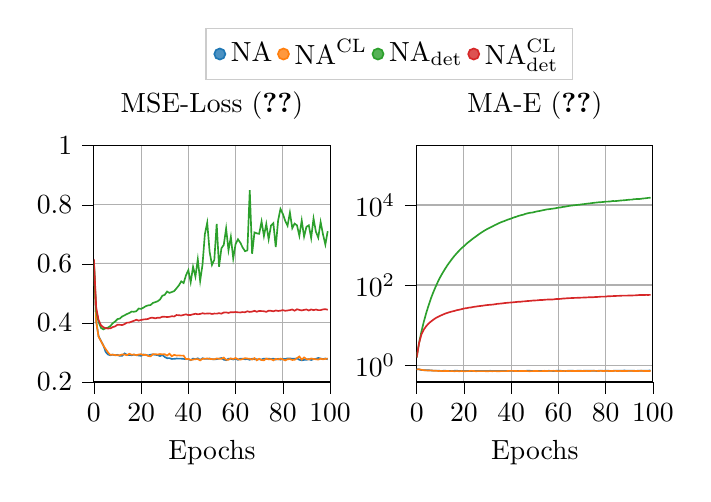
\begin{tikzpicture}

\definecolor{crimson2143940}{RGB}{214,39,40}
\definecolor{darkgray176}{RGB}{176,176,176}
\definecolor{darkorange25512714}{RGB}{255,127,14}
\definecolor{forestgreen4416044}{RGB}{44,160,44}
\definecolor{lightgray204}{RGB}{204,204,204}
\definecolor{steelblue31119180}{RGB}{31,119,180}

\begin{axis}[
name = plot1,
    width=3cm,  % Adjust the width of the plot
    height=3cm,  % Adjust the height of the plot
    scale only axis, 
    xlabel={Epochs},
legend cell align={center},
legend style={
  fill opacity=0.8,
  draw opacity=1,
  text opacity=1,
  at={(1.25,1.5)},
  anchor=north,
  draw=lightgray204,
  legend columns = -1
  mark=*
},
legend image code/.code={
        \draw[mark options={scale=1}, mark=*] plot coordinates {(0.3cm,0cm)}; % Use points in the legend
    },
tick align=outside,
tick pos=left,
x grid style={darkgray176},
xmajorgrids,
xmin=0, xmax=100,
xtick style={color=black},
y grid style={darkgray176},
ylabel={},
title={MSE-Loss (\ref{equ:MSELoss})},
ymajorgrids,
ymin=0.2, 
ymax=1,
ytick style={color=black},
]
\addplot [semithick, steelblue31119180]
table {%
0 0.611941409394145
1 0.404460925444961
2 0.355163639776409
3 0.339247392460704
4 0.324812070466578
5 0.301795873902738
6 0.292822175815701
7 0.290735897243023
8 0.292805431999266
9 0.290305355966091
10 0.291941600158811
11 0.288333343707025
12 0.288737422563136
13 0.296677809603512
14 0.292281404785812
15 0.290858758054674
16 0.290767313160002
17 0.292714920699596
18 0.290587794758379
19 0.289766863293946
20 0.288406750351191
21 0.293193183898926
22 0.291701209932566
23 0.290007071204483
24 0.292503394111991
25 0.293332264944911
26 0.291972432099283
27 0.291046844929457
28 0.287716829553247
29 0.291602838911116
30 0.284840544752777
31 0.280512229338288
32 0.280809077531099
33 0.277989823311567
34 0.278361989110708
35 0.279393471904099
36 0.279003665581346
37 0.279020595915616
38 0.278237650796771
39 0.277349738404155
40 0.277278342619538
41 0.273919279158115
42 0.279123209051788
43 0.27709675514698
44 0.28020255998522
45 0.27470947098732
46 0.280286003962159
47 0.27813413977623
48 0.278169064290822
49 0.279392674587667
50 0.277171799391508
51 0.276486691772938
52 0.277413161180913
53 0.279150147378445
54 0.281031813181937
55 0.275608771234751
56 0.27366885086149
57 0.279172012083232
58 0.278515524618328
59 0.276100231125951
60 0.278760932698846
61 0.275043711975217
62 0.279179656289518
63 0.278528353877366
64 0.276965564243495
65 0.277563843168318
66 0.275165799811482
67 0.2789791867733
68 0.276749472655356
69 0.276790994957089
70 0.276459479801357
71 0.276327098228037
72 0.279078826345503
73 0.27826146197319
74 0.278874768920243
75 0.277815463848412
76 0.278804229311645
77 0.275874389119446
78 0.278570503793657
79 0.275502957567573
80 0.278709277048707
81 0.277353476390243
82 0.280052238218486
83 0.279736127734184
84 0.278723088487983
85 0.278621223472059
86 0.279907686054707
87 0.275282921276987
88 0.273415324039757
89 0.274746660880744
90 0.274893422745168
91 0.277455612197518
92 0.274458181723952
93 0.277263621002436
94 0.278553314588964
95 0.281348010055721
96 0.279461028672755
97 0.277654385901988
98 0.279517267264426
99 0.276829372189939
};
\addlegendentry{$\text{NA}$}
\addplot [semithick, darkorange25512714]
table {%
0 0.608796063810587
1 0.404834068283439
2 0.353451243817806
3 0.338568493880332
4 0.323459391139448
5 0.311533840574324
6 0.300045564420521
7 0.291719058051705
8 0.292339117482305
9 0.291288265392184
10 0.290410711705685
11 0.290524671278894
12 0.293199801497161
13 0.293025554820895
14 0.290531463526189
15 0.295489782825112
16 0.292294562637806
17 0.292943701155484
18 0.290817392267287
19 0.293005076251924
20 0.294164174884558
21 0.291099690787494
22 0.292309767723083
23 0.288032758355141
24 0.286823302768171
25 0.293853967666626
26 0.294363110654056
27 0.292947210237384
28 0.294658658236265
29 0.293523136638105
30 0.293943503648043
31 0.289424084164202
32 0.295608305335045
33 0.287112329237163
34 0.291889309346676
35 0.289596081763506
36 0.290031305097044
37 0.289163750000298
38 0.289397771321237
39 0.277202979832888
40 0.278286978907883
41 0.274547535397112
42 0.275911723800004
43 0.277363488964736
44 0.277568548239768
45 0.273078170023859
46 0.278599904976785
47 0.278825132340193
48 0.279550102636218
49 0.278170816399157
50 0.277482765451074
51 0.276931995548308
52 0.27972166389972
53 0.278546011075377
54 0.278506645992398
55 0.282398849375546
56 0.275060715161264
57 0.275370138250291
58 0.279895563319325
59 0.277708165705204
60 0.281192395374179
61 0.27682488746196
62 0.275595603443682
63 0.277571296684444
64 0.280766646973789
65 0.27943359337002
66 0.278589633107185
67 0.275965581551194
68 0.280830531902611
69 0.273645771220326
70 0.278702991873026
71 0.274352182485163
72 0.273271102510393
73 0.27945484072715
74 0.276404253445566
75 0.277227476261556
76 0.273234584100544
77 0.278205651275814
78 0.276227233588696
79 0.279279652908444
80 0.276720661975443
81 0.273039626404643
82 0.276899457156658
83 0.277564294412732
84 0.274600497633219
85 0.27512222328037
86 0.280471811644733
87 0.286434203542769
88 0.275768381729722
89 0.283131299182773
90 0.277525585323572
91 0.276315912701189
92 0.279433982238174
93 0.277927031427622
94 0.276872227557004
95 0.275729609794915
96 0.278945564739406
97 0.276855052880943
98 0.278311800837517
99 0.279406821645796
};
\addlegendentry{$\text{NA}^\text{CL}$}
\addplot [semithick, forestgreen4416044]
table {%
0 0.611609450370073
1 0.439915159359574
2 0.402905011504889
3 0.383407583221793
4 0.378339802965522
5 0.382299789071083
6 0.384070707291365
7 0.389385624021292
8 0.399069177210331
9 0.404827949911356
10 0.412929787904024
11 0.414823229983449
12 0.421921906873584
13 0.425825444385409
14 0.43003033643961
15 0.433517695590854
16 0.438393251121044
17 0.437865211963654
18 0.439733000442386
19 0.448825848251581
20 0.44746831817925
21 0.451768790438771
22 0.456774653479457
23 0.459475716635585
24 0.460669831678271
25 0.467696123689413
26 0.470393957212567
27 0.47330911564827
28 0.479266878798604
29 0.492035465598106
30 0.495099705278873
31 0.506255769014359
32 0.501853556618094
33 0.504647214472294
34 0.507795336171985
35 0.517213715299964
36 0.527184344947338
37 0.540708477377892
38 0.535105723246932
39 0.561149383425713
40 0.57866429579258
41 0.53783510453999
42 0.590163114398718
43 0.557026644676924
44 0.61548131018877
45 0.54224068044126
46 0.597406392633915
47 0.700817015364766
48 0.739486065238714
49 0.64181193523109
50 0.59636370061338
51 0.614021787241101
52 0.735419025689363
53 0.590475044742227
54 0.652752056062222
55 0.664430199787021
56 0.720020437479019
57 0.646270394340158
58 0.691383462801576
59 0.618400651171803
60 0.667103306367993
61 0.683399421453476
62 0.671754186838865
63 0.655481513738632
64 0.642903120398521
65 0.645933763623238
66 0.849703469723463
67 0.634023216992617
68 0.706610255494714
69 0.70335243485868
70 0.701880310982466
71 0.743811122655869
72 0.694135029777884
73 0.734894439533353
74 0.683351158410311
75 0.729692776799202
76 0.737865243852138
77 0.656588634103537
78 0.746453127741814
79 0.786057748436928
80 0.769413703620434
81 0.746070098757744
82 0.729212529271841
83 0.773686207860708
84 0.720844190388918
85 0.736456541448832
86 0.730318913727999
87 0.695238190889359
88 0.747054092675447
89 0.69227656596899
90 0.725485775560141
91 0.730593508601189
92 0.687429808497429
93 0.753641017556191
94 0.709013304740191
95 0.688680979758501
96 0.741845514267683
97 0.700211458534002
98 0.665500582426786
99 0.710758947059512
};
\addlegendentry{$\text{NA}_\text{det}$}
\addplot [semithick, crimson2143940]
table {%
0 0.61643166154623
1 0.451805842861533
2 0.409961090907454
3 0.392075737953186
4 0.385575036212802
5 0.382028292134404
6 0.381157822176814
7 0.381767434999347
8 0.385939629092813
9 0.388244169682264
10 0.394128766864538
11 0.393550968199968
12 0.392839833676815
13 0.396085587128997
14 0.400960114747286
15 0.401235269933939
16 0.404315443471074
17 0.40736368817091
18 0.410646104961634
19 0.407733978703618
20 0.410043139457703
21 0.41177126955986
22 0.412383782222867
23 0.413597009524703
24 0.417239158540964
25 0.417437488898635
26 0.415505234986544
27 0.417706749945879
28 0.417414122521877
29 0.421165493309498
30 0.420716576308012
31 0.420093193635345
32 0.420569443538785
33 0.422663229003549
34 0.421872788339853
35 0.426678671315312
36 0.426079013392329
37 0.425104559883475
38 0.42722222545743
39 0.429121752738953
40 0.42655730958283
41 0.427006248027086
42 0.429205042302608
43 0.430995577126741
44 0.429385351166129
45 0.430380379512906
46 0.432773048639297
47 0.431285184592009
48 0.431893689617515
49 0.432349317163229
50 0.430300185695291
51 0.431707549676299
52 0.431425787881017
53 0.433075299277902
54 0.431460279360414
55 0.435230349957943
56 0.435780043512583
57 0.433873699858785
58 0.436460872322321
59 0.436038340106606
60 0.436940508961678
61 0.435898477628827
62 0.435486101523042
63 0.436774514377117
64 0.436168460130692
65 0.439455194503069
66 0.43727204246819
67 0.438427097216249
68 0.440966750845313
69 0.437848162785172
70 0.440606507360935
71 0.440070451557636
72 0.439671826213598
73 0.437487634658813
74 0.441459807395935
75 0.441003379151225
76 0.439396331682801
77 0.442133032754064
78 0.44050989998877
79 0.441478393092751
80 0.443431491866708
81 0.441017071440816
82 0.442220961645246
83 0.443517910316586
84 0.445675541892648
85 0.441425472855568
86 0.446285691589117
87 0.444073230117559
88 0.442379747524858
89 0.444188039451838
90 0.445629195898771
91 0.442071973070502
92 0.445623260036111
93 0.443225308865309
94 0.445463816702366
95 0.443319242119789
96 0.443458917245269
97 0.445811537995934
98 0.446655088037252
99 0.444551042348146
};
\addlegendentry{$\text{NA}^\text{CL}_\text{det}$}
\end{axis}

\begin{axis}[
        at={(plot1.east)}, % Align it next to the first plo
    anchor=west,
    width=3cm,  % Adjust the width of the plot
    height=3cm,  % Adjust 
     xshift=1.1cm, %the height of the plot
    scale only axis, 
     title={MA-E (\ref{equ:MAE})},
log basis y={10},
tick align=outside,
tick pos=left,
x grid style={darkgray176},
xlabel={Epochs},
xmajorgrids,
xmin=0, xmax=100,
xtick style={color=black},
y grid style={darkgray176},
ymajorgrids,
ymin=0.37772735089694, ymax=302220.574977491,
ymode=log,
ytick style={color=black}
]
\addplot [semithick, steelblue31119180]
table {%
0 0.784316565593084
1 0.781134277582169
2 0.75108015537262
3 0.747364002466202
4 0.740072242418925
5 0.742147266864777
6 0.734453016519547
7 0.725739912192027
8 0.725482821464539
9 0.725872256358465
10 0.71623806754748
11 0.717047673463821
12 0.724361884593964
13 0.710147565603256
14 0.71484912832578
15 0.710747335354487
16 0.718673286835353
17 0.720987143119176
18 0.712739396095276
19 0.71228361527125
20 0.712281819184621
21 0.708043175935745
22 0.713457111517588
23 0.707725787162781
24 0.710828079779943
25 0.710757700602214
26 0.708714254697164
27 0.707544475793839
28 0.710333482424418
29 0.71262610356013
30 0.712401813268661
31 0.718252156178157
32 0.716661332050959
33 0.71257671713829
34 0.714103603363037
35 0.715125119686127
36 0.717597754796346
37 0.71170742114385
38 0.715586141745249
39 0.713813449939092
40 0.716613757610321
41 0.713593037923177
42 0.712899752457937
43 0.716273045539856
44 0.716301995515823
45 0.71634173989296
46 0.715151470899582
47 0.720994468530019
48 0.719423288106918
49 0.709180527925491
50 0.714239386717478
51 0.714714256922404
52 0.716577911376953
53 0.715655094385147
54 0.718004085620244
55 0.715379571914673
56 0.718934539953868
57 0.715375073750814
58 0.7126762231191
59 0.718821219603221
60 0.718017041683197
61 0.718857727448146
62 0.714162311951319
63 0.712864913543065
64 0.719291679064433
65 0.722002234061559
66 0.721423623959223
67 0.712879719336828
68 0.719574244817098
69 0.722789339224498
70 0.716404211521149
71 0.719432612260183
72 0.722413490215937
73 0.71859184106191
74 0.722885553042094
75 0.721519402662913
76 0.712608919541041
77 0.720148783922195
78 0.72747211654981
79 0.716309491793315
80 0.723044633865356
81 0.720361840724945
82 0.716077470779419
83 0.715186387300491
84 0.727467252810796
85 0.722101583083471
86 0.71787742972374
87 0.724995827674866
88 0.730283008019129
89 0.718816594282786
90 0.718360368410746
91 0.722093685468038
92 0.71898397008578
93 0.715825537840525
94 0.726787326733271
95 0.721089694897334
96 0.722597585121791
97 0.723732564846675
98 0.724596387147903
99 0.73590941230456
};
\addplot [semithick, darkorange25512714]
table {%
0 0.780062007904053
1 0.785003300507863
2 0.760595844189326
3 0.743645322322845
4 0.738197988271713
5 0.727404369910558
6 0.73832106590271
7 0.720802754163742
8 0.72067355910937
9 0.713183629512787
10 0.71515442331632
11 0.705765650669734
12 0.712433300415675
13 0.712155882517497
14 0.704875973860423
15 0.708641225099564
16 0.70104883313179
17 0.708326105276744
18 0.701419488588969
19 0.70841281414032
20 0.702454942464829
21 0.704174659649531
22 0.704577163855235
23 0.717927555243174
24 0.71203598578771
25 0.70237233042717
26 0.705128888289134
27 0.707403345902761
28 0.706829740603765
29 0.703698541720708
30 0.700653398036957
31 0.706547838449478
32 0.703005766868591
33 0.707197372118632
34 0.701774646838506
35 0.702649648984273
36 0.705712916453679
37 0.705201524496079
38 0.706422601143519
39 0.714035723606745
40 0.718191597859065
41 0.714887227614721
42 0.710324345032374
43 0.705266364415487
44 0.713340729475021
45 0.710121959447861
46 0.713599592447281
47 0.704361832141876
48 0.703318081299464
49 0.707208555936813
50 0.708930063247681
51 0.708541176716487
52 0.706024523576101
53 0.706982847054799
54 0.713527637720108
55 0.712104618549347
56 0.715284230311712
57 0.714014929533005
58 0.718396516640981
59 0.712120225032171
60 0.70300657749176
61 0.712330993016561
62 0.705399974187215
63 0.716652369499207
64 0.711654380957286
65 0.715257356564204
66 0.709045793612798
67 0.710406134525935
68 0.713286699851354
69 0.713970551888148
70 0.714134921630224
71 0.708393577734629
72 0.71591382821401
73 0.708847548564275
74 0.716458161671956
75 0.717960963646571
76 0.716552470127741
77 0.71113104224205
78 0.718919990460078
79 0.707574218511581
80 0.714642171065013
81 0.714416901270548
82 0.706916064023972
83 0.711730722586314
84 0.718201941251755
85 0.708433689673742
86 0.716953217983246
87 0.710274974505107
88 0.712638219197591
89 0.712405643860499
90 0.717525462309519
91 0.716002144416173
92 0.711754639943441
93 0.713744324445724
94 0.711945599317551
95 0.720099818706512
96 0.712131476402283
97 0.712278308471044
98 0.713869651158651
99 0.712531715631485
};
\addplot [semithick, forestgreen4416044]
table {%
0 1.55465695460637
1 3.54276961485545
2 6.84717055956523
3 11.9553510348002
4 19.6561587651571
5 30.3932488759359
6 45.8300317128499
7 65.1476365407308
8 89.9160723368327
9 120.983692932129
10 158.812667338053
11 201.779645284017
12 252.178554789225
13 311.822377522786
14 377.131458536784
15 452.17714436849
16 537.134820556641
17 626.936676025391
18 724.715093994141
19 833.412182617187
20 933.673201497396
21 1062.58614298503
22 1190.99056803385
23 1323.37373046875
24 1475.06894124349
25 1623.04679361979
26 1796.58349609375
27 1975.16912434896
28 2162.06663411458
29 2351.95164794922
30 2534.69059651693
31 2714.21853841146
32 2902.59532877604
33 3122.97405598958
34 3328.1301188151
35 3555.73961588542
36 3765.49230957031
37 3952.48976236979
38 4180.17137858073
39 4398.964453125
40 4583.77263997396
41 4859.77096354167
42 5055.92880045573
43 5308.26098632812
44 5534.4049235026
45 5709.12517903646
46 5985.44622395833
47 6210.53883463542
48 6397.46751302083
49 6480.77866210937
50 6707.73958333333
51 6937.21790364583
52 7081.87277018229
53 7304.57184244792
54 7511.70415039062
55 7744.83385416667
56 7863.42859700521
57 8010.54152018229
58 8161.38434244792
59 8352.13855794271
60 8576.60143229167
61 8720.91819661458
62 8963.25335286458
63 9117.78852539062
64 9383.36124674479
65 9600.45442708333
66 9750.65011393229
67 9912.16370442708
68 10039.796891276
69 10187.0822428385
70 10414.3989257812
71 10564.920296224
72 10784.1141113281
73 10934.0772298177
74 11117.7188639323
75 11350.2178710937
76 11500.594905599
77 11680.1168945312
78 11773.5132161458
79 11925.4419596354
80 12148.5900065104
81 12169.8748046875
82 12290.8735026042
83 12554.8247395833
84 12507.3008463542
85 12676.0856770833
86 12885.6792317708
87 13032.0627278646
88 13163.2922851563
89 13345.2062825521
90 13582.3030924479
91 13619.6559244792
92 13966.8358723958
93 14086.3044270833
94 14076.3888671875
95 14291.4867838542
96 14588.037890625
97 14730.4602864583
98 15068.0731119792
99 15193.1791666667
};
\addplot [semithick, crimson2143940]
table {%
0 1.54190982580185
1 3.52118768692017
2 5.78630299568176
3 7.67343028386434
4 9.32714433670044
5 10.8580426216125
6 12.2028846740723
7 13.5414336204529
8 14.8556263923645
9 16.017956829071
10 17.1215937614441
11 18.1431117375692
12 19.2817598342896
13 20.121834564209
14 21.0518109639486
15 21.8852607727051
16 22.524635887146
17 23.5350463867188
18 24.1527964274089
19 24.9533289591471
20 25.9407367070516
21 26.3416049957275
22 27.1657480875651
23 27.5096417109172
24 28.3973735173543
25 28.8585123697917
26 29.5232582092285
27 29.9796120325724
28 30.5138794581095
29 31.1672804514567
30 31.6722736358643
31 32.1286259333293
32 32.4027076085409
33 32.9874686559041
34 33.7719740549723
35 34.2146395365397
36 34.6404315948486
37 35.3181519826253
38 35.8040141423543
39 36.2991956710815
40 36.5904066085815
41 37.1327234903971
42 37.5759311040242
43 38.1746032714844
44 38.2666483561198
45 38.9697507222494
46 39.2302190144857
47 39.9760008494059
48 40.1718897501628
49 40.8396077473958
50 41.1574705759684
51 41.4496417999268
52 42.11405321757
53 42.1532773335775
54 42.8213433583577
55 43.2922027587891
56 43.3367314656576
57 43.3879510243734
58 43.8423197428385
59 44.7495100657145
60 44.7827958424886
61 45.1918746948242
62 46.013836924235
63 46.3216091156006
64 46.8736853281657
65 47.1226577758789
66 47.4211101531982
67 47.7491437276204
68 47.9290562947591
69 48.2311442057292
70 48.5239919026693
71 48.7080121358236
72 49.0425851186117
73 49.4799237569173
74 49.343957010905
75 49.7897899627686
76 50.324275080363
77 50.5796007792155
78 51.2719327290853
79 51.2950219472249
80 51.5075139363607
81 52.4433975219727
82 52.6479281107585
83 52.910989634196
84 53.265039952596
85 53.6047564188639
86 53.7609555562337
87 54.2889787038167
88 54.3406288146973
89 54.391259765625
90 54.7481624603272
91 54.9078276316325
92 55.0772015889486
93 55.4503991444906
94 56.1480810801188
95 56.5388488769531
96 56.1639583587646
97 56.6805483500163
98 56.5415815989176
99 56.8630076090495
};

\end{axis}

\end{tikzpicture}

    \caption{Training \gls{MSE} and \gls{MA-E} when using \gls{NA} for training with and without \gls{CL}. We compare training using detached and attached noise as in (\ref{equ:NAdet}) and (\ref{equ:classicNA}), respectively. In the \gls{MA-E}, NA and $\text{NA}_\text{det}$ overlap.}
    \label{fig:NIdetvsat}
\end{figure}
\begin{figure}[t]
    \centering
    % This file was created with tikzplotlib v0.10.1.
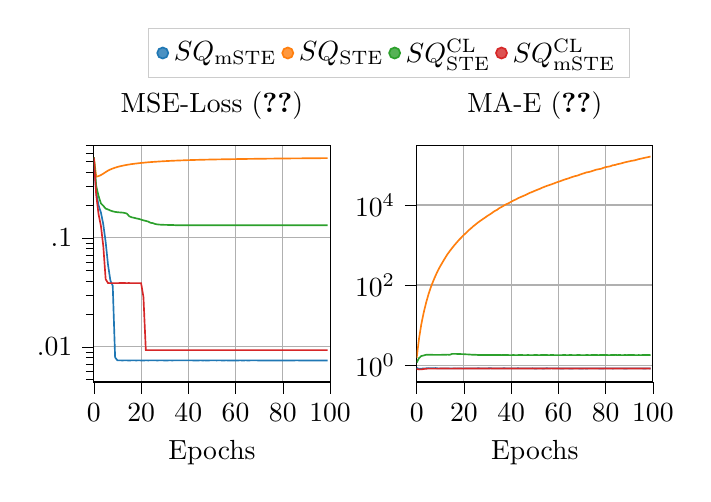
\begin{tikzpicture}

\definecolor{crimson2143940}{RGB}{214,39,40}
\definecolor{darkgray176}{RGB}{176,176,176}
\definecolor{darkorange25512714}{RGB}{255,127,14}
\definecolor{forestgreen4416044}{RGB}{44,160,44}
\definecolor{lightgray204}{RGB}{204,204,204}
\definecolor{steelblue31119180}{RGB}{31,119,180}

\begin{axis}[
ymode = log,
yticklabels={,.01,.1},
name = plot1,
    width=3cm,  % Adjust the width of the plot
    height=3cm,  % Adjust the height of the plot
    scale only axis, 
    xlabel={Epochs},
legend cell align={center},
legend style={
  fill opacity=0.8,
  draw opacity=1,
  text opacity=1,
  at={(1.25,1.5)},
  anchor=north,
  draw=lightgray204,
  legend columns = -1
  mark=*
},
legend image code/.code={
        \draw[mark options={scale=1}, mark=*] plot coordinates {(0.3cm,0cm)}; % Use points in the legend
    },
tick align=outside,
tick pos=left,
x grid style={darkgray176},
xmajorgrids,
xmin=0, xmax=100,
xtick style={color=black},
y grid style={darkgray176},
ylabel={},
title={MSE-Loss (\ref{equ:MSELoss})},
ymajorgrids,
ymin=0, 
ymax=0.7,
ytick style={color=black},
]
\addplot [semithick, steelblue31119180]
table {%
0 0.548415012225509
1 0.260596112176776
2 0.199333541236818
3 0.170763516455889
4 0.132872804656625
5 0.0918383099529892
6 0.0567078236807138
7 0.0406543923430145
8 0.0363865633243695
9 0.00801322893449105
10 0.00752538197487593
11 0.00752483715652488
12 0.00752032087184489
13 0.00752312026103027
14 0.00752570083457977
15 0.0075128314960748
16 0.00752777750534005
17 0.00752507122093812
18 0.00752093595499173
19 0.00752727594855241
20 0.00752138263569213
21 0.00751542641315609
22 0.00752721480140462
23 0.007520337237278
24 0.00752563506388105
25 0.00753043382498436
26 0.00752470010262914
27 0.00752017146185972
28 0.00752917782124132
29 0.00752881077281199
30 0.00751396194892004
31 0.00751694584148936
32 0.00752815241133794
33 0.00752066366304643
34 0.00752370889740996
35 0.0075245041269809
36 0.00752782307215966
37 0.00752837221557274
38 0.00752370861545205
39 0.00753300691070035
40 0.00752386529557407
41 0.00752627824433148
42 0.00752069049724378
43 0.00751482116989791
44 0.00750940577406436
45 0.00752902232459746
46 0.00751835922966711
47 0.00752379640331492
48 0.00751147268363275
49 0.00752187384222634
50 0.00753117379080504
51 0.00753021406545304
52 0.00752012984850444
53 0.00753299265610985
54 0.00752129695983604
55 0.00751948116952553
56 0.00752447230764665
57 0.00751921636611223
58 0.00751629655295983
59 0.00751851693820208
60 0.00751744952122681
61 0.00751953963609412
62 0.00752549178292975
63 0.00751764936535619
64 0.00752256043767557
65 0.00752234915737063
66 0.00752038859669119
67 0.00753002483327873
68 0.00752449164609425
69 0.00752483649901114
70 0.00751591556938365
71 0.00752251353464089
72 0.00751609408552758
73 0.00751590899424627
74 0.00751730271382257
75 0.00751301128650084
76 0.00752065231674351
77 0.0075163100764621
78 0.00752277068328112
79 0.0075161181895528
80 0.00752222670963965
81 0.00751390267442912
82 0.00751506595872343
83 0.0075175651377067
84 0.00751211134647019
85 0.00751949909585528
86 0.00753027279488742
87 0.00751712884264998
88 0.00751450412650593
89 0.00751784336776473
90 0.0075144024589099
91 0.00751551885413937
92 0.0075192875280045
93 0.0075173814680893
94 0.00750582735124044
95 0.00751378774479963
96 0.00751508517912589
97 0.00751278982986696
98 0.00750667718774639
99 0.00751805932610296
};
\addlegendentry{$SQ_\text{mSTE}$}
\addplot [semithick, darkorange25512714]
table {%
0 0.55088772341609
1 0.364599603518844
2 0.368866781711578
3 0.377288254261017
4 0.388566744953394
5 0.401835393205285
6 0.414005573749542
7 0.424335187733173
8 0.433307941555977
9 0.440919484496117
10 0.447635944843292
11 0.453682038679719
12 0.458860293194652
13 0.463521628290415
14 0.467869847580791
15 0.471703230798244
16 0.475401790723205
17 0.478585365355015
18 0.481512870833278
19 0.484425481408834
20 0.487144548967481
21 0.489412767782807
22 0.491777189701796
23 0.493936263769865
24 0.495904034361243
25 0.497762332350016
26 0.499550337582827
27 0.501130907699466
28 0.502885586768389
29 0.504318796187639
30 0.505741798982024
31 0.507270608186722
32 0.508436697110534
33 0.509720933899283
34 0.510865337014198
35 0.511979941368103
36 0.513019118696451
37 0.513959438443184
38 0.514955953866243
39 0.516012669444084
40 0.516867266148329
41 0.517744843870401
42 0.51857935076952
43 0.519320396065712
44 0.519961907505989
45 0.520658597141504
46 0.521395146280527
47 0.521903126507998
48 0.522700056582689
49 0.52323027163744
50 0.523826842874289
51 0.524266020983458
52 0.524801029682159
53 0.525233933061361
54 0.525834440082312
55 0.526259167104959
56 0.526617806315422
57 0.527145440518856
58 0.527537268251181
59 0.527885058254004
60 0.528327745348215
61 0.52878401529789
62 0.529222670078278
63 0.529591565400362
64 0.529899104863405
65 0.530336342602968
66 0.530688235938549
67 0.530990009218454
68 0.531487732738256
69 0.531842892467976
70 0.532275775909424
71 0.532542983800173
72 0.532737836956978
73 0.533120610415936
74 0.533493458986282
75 0.533814318478107
76 0.534058399617672
77 0.534519419878721
78 0.534666323184967
79 0.534989660829306
80 0.535261952996254
81 0.535537146002054
82 0.535684410214424
83 0.535837888389826
84 0.536177230507135
85 0.53638651779294
86 0.536517620921135
87 0.536831999242306
88 0.536970202863216
89 0.537155061453581
90 0.537432105869055
91 0.53773717880249
92 0.53779073548317
93 0.538084347188473
94 0.538191051691771
95 0.53855269575119
96 0.53880144482851
97 0.538929655462503
98 0.5389938133955
99 0.539319223552942
};
\addlegendentry{$SQ_\text{STE}$}
\addplot [semithick, forestgreen4416044]
table {%
0 0.549000259801745
1 0.299871038094163
2 0.242189251571894
3 0.207308624267578
4 0.197074625216424
5 0.185634178325534
6 0.182380964674056
7 0.178326630882919
8 0.175201226659119
9 0.173283803023398
10 0.172094418533146
11 0.171343371406198
12 0.170765378408134
13 0.169521951183677
14 0.167103111922741
15 0.157875367105007
16 0.154614733763039
17 0.153081586278975
18 0.150951494216919
19 0.149476350657642
20 0.147199265860021
21 0.144910294152796
22 0.143213532932103
23 0.14128946762532
24 0.137701354525983
25 0.136567906014621
26 0.134132204532623
27 0.132960757054389
28 0.132355139888823
29 0.131965770825744
30 0.131745044507086
31 0.131587471209466
32 0.13147689602524
33 0.131349040202796
34 0.131103035457432
35 0.130517799466848
36 0.130464115925133
37 0.130513427942991
38 0.130506151787937
39 0.130541185207665
40 0.130534353867173
41 0.130492865376174
42 0.130522380650043
43 0.130526529125869
44 0.130550112396479
45 0.130531256340444
46 0.130503811851144
47 0.130515778191388
48 0.130510073944926
49 0.130536538757384
50 0.130526625037193
51 0.130501929484308
52 0.130520934864879
53 0.130509537316859
54 0.130512963078916
55 0.130522072032094
56 0.130513535268605
57 0.130511100739241
58 0.130539780512452
59 0.130513597756624
60 0.130501266375184
61 0.130528594397008
62 0.130528959475458
63 0.130543941237032
64 0.130528621524572
65 0.130521844916046
66 0.130523137196898
67 0.130502953402698
68 0.130502688154578
69 0.130511386707425
70 0.130524727001786
71 0.130521879352629
72 0.130487557888031
73 0.130523864358664
74 0.130489279292524
75 0.130496246568859
76 0.130508339770138
77 0.130523177161813
78 0.130494157969952
79 0.130501418083906
80 0.130529735192657
81 0.130518131420016
82 0.130508684828877
83 0.130500476054847
84 0.130506072625518
85 0.130520362116396
86 0.13052210765332
87 0.130500621564686
88 0.130523995541036
89 0.130495601221919
90 0.130508861780167
91 0.130531919181347
92 0.130510828539729
93 0.130509101711214
94 0.130512753784657
95 0.130492839120328
96 0.130500469848514
97 0.130490967720747
98 0.130495262987912
99 0.130493671834469
};
\addlegendentry{$SQ_\text{STE}^\text{CL}$}
\addplot [semithick, crimson2143940]
table {%
0 0.544153192952275
1 0.248425985530019
2 0.164691873550415
3 0.128648992173374
4 0.0838899204917252
5 0.0417874237690121
6 0.0385444990582764
7 0.0385049095787108
8 0.0384967143498361
9 0.0385195656865835
10 0.0385160425622016
11 0.0385357322134078
12 0.038534109480679
13 0.0385317649245262
14 0.0385209232810885
15 0.0385310827456415
16 0.0384953307788819
17 0.0384952042140067
18 0.0385053486600518
19 0.0385036334935576
20 0.0384773015771061
21 0.0286449612174183
22 0.00934916036436334
23 0.00934722829656675
24 0.00934804730443284
25 0.00934688501665369
26 0.00934892255626619
27 0.00935017336159944
28 0.00935114128375426
29 0.00934771656431258
30 0.00934540102351457
31 0.00935453312192112
32 0.00935013657994568
33 0.00934792333096266
34 0.00934989839419723
35 0.00935237167496234
36 0.00934469219530001
37 0.0093483248539269
38 0.00935291248885915
39 0.00934915019385517
40 0.00934571000235155
41 0.00934837823081762
42 0.00934899662155658
43 0.00935033038724214
44 0.00934421865548938
45 0.00934903470706195
46 0.00934945413237438
47 0.00934787023393437
48 0.00934440769907087
49 0.00934540874511004
50 0.00935275487368926
51 0.00935078661795706
52 0.00934717530291528
53 0.009345349971205
54 0.00935187224624679
55 0.00934593824390322
56 0.00934900092938915
57 0.00934595982916653
58 0.00934418482193723
59 0.00935198008688167
60 0.00935088515095413
61 0.00934546708734706
62 0.00934788803616539
63 0.00934711833763868
64 0.00935056802397594
65 0.00934861720679328
66 0.00934991103224456
67 0.00934911843948066
68 0.00934640683792532
69 0.00934659997047856
70 0.00935074001271278
71 0.00934409358212724
72 0.00934975521126762
73 0.00935268123727292
74 0.00934827431710437
75 0.00934959468618035
76 0.0093522864584811
77 0.00935016064764932
78 0.00935106620984152
79 0.00934808949381113
80 0.00934725726908073
81 0.00935152086615562
82 0.00934670987585559
83 0.00935189650719985
84 0.00934574100933969
85 0.00934906351426616
86 0.00935401551006362
87 0.00935002066288143
88 0.00934754252713174
89 0.00934870791714638
90 0.00935289056319743
91 0.00934692508447915
92 0.00934829985210672
93 0.00935069577442482
94 0.00934891671128571
95 0.00934632327081636
96 0.00935236550169066
97 0.00934587485063821
98 0.00935068418178707
99 0.00934836278343573
};
\addlegendentry{$SQ_\text{mSTE}^\text{CL}$}
\end{axis}


\begin{axis}[
        at={(plot1.east)}, % Align it next to the first plot
    anchor=west,
    width=3cm,  % Adjust the width of the plot
    height=3cm,  % Adjust 
     xshift=1.1cm, %the height of the plot
    scale only axis, 
  title={MA-E (\ref{equ:MAE})},
log basis y={10},
tick align=outside,
tick pos=left,
x grid style={darkgray176},
xlabel={Epochs},
xmajorgrids,
xmin=0, xmax=100,
xtick style={color=black},
y grid style={darkgray176},
ymajorgrids,
ymin=0.37772735089694, ymax=302220.574977491,
ymode=log,
ytick style={color=black}
]
\addplot [semithick, steelblue31119180]
table {%
0 0.851375661293666
1 0.806172464291255
2 0.812832925717036
3 0.827050844828288
4 0.828881853818893
5 0.839782045284907
6 0.837877966960271
7 0.839749137560526
8 0.841935312747955
9 0.827198886871338
10 0.829452168941498
11 0.828425870339076
12 0.828687649965286
13 0.828649872541428
14 0.828402545054754
15 0.829283454020818
16 0.829582351446152
17 0.827392035722733
18 0.827296247084936
19 0.826385231812795
20 0.825873935222626
21 0.826272092262904
22 0.829095045725505
23 0.828043138980865
24 0.829359706242879
25 0.825448644161224
26 0.831103394428889
27 0.82834423383077
28 0.827774888277054
29 0.826178681850433
30 0.82883224884669
31 0.832357136408488
32 0.828405461708705
33 0.827094235022863
34 0.827335288127263
35 0.828002520402273
36 0.827962724367778
37 0.8313736140728
38 0.827159323294957
39 0.828334468603134
40 0.828757450977961
41 0.829585385322571
42 0.828349604209264
43 0.8305335521698
44 0.826499412457148
45 0.825795143842697
46 0.826147758960724
47 0.826950929562251
48 0.825480167071025
49 0.829947408040365
50 0.823849985996882
51 0.825413328409195
52 0.828409097592036
53 0.825286384423574
54 0.823809057474136
55 0.83239281574885
56 0.826397462685903
57 0.826078220208486
58 0.82554986278216
59 0.829379457235336
60 0.828008983532588
61 0.823278741041819
62 0.823613027731578
63 0.828036558628082
64 0.826531108220418
65 0.822369156281153
66 0.823448852698008
67 0.829317446549733
68 0.828767079114914
69 0.822965995470683
70 0.824071802695592
71 0.826074622074763
72 0.823374515771866
73 0.828081520398458
74 0.827080847819646
75 0.826028686761856
76 0.827883988618851
77 0.825355138381322
78 0.821851378679275
79 0.822457506259282
80 0.829773046573003
81 0.826981800794601
82 0.827518127361933
83 0.82455484867096
84 0.826452980438868
85 0.828788681825002
86 0.825748177369436
87 0.827113646268845
88 0.823399613300959
89 0.825183908144633
90 0.82611332933108
91 0.826250165700912
92 0.827026361227036
93 0.826306056976318
94 0.828172109524409
95 0.826435246070226
96 0.824748667081197
97 0.824827434619268
98 0.827027906974157
99 0.82360468506813
};
\addplot [semithick, darkorange25512714]
table {%
0 1.52191224098206
1 4.62942314147949
2 10.7700797080994
3 20.8528925577799
4 36.3747828801473
5 58.6029336293538
6 88.5621025085449
7 125.331676737467
8 172.717534383138
9 231.091755167643
10 297.690074666341
11 374.748385620117
12 470.715333048503
13 584.981895955404
14 705.257332356771
15 840.939318847656
16 996.562082926432
17 1164.62107543945
18 1361.14012451172
19 1563.32934977214
20 1795.80465087891
21 2030.06355794271
22 2333.39939778646
23 2611.14085286458
24 2954.9336710612
25 3288.2523844401
26 3671.10323079427
27 4043.10830891927
28 4452.31261393229
29 4877.00172526042
30 5379.12698567708
31 5833.47943522135
32 6415.72179361979
33 7065.05356445312
34 7571.12750651042
35 8357.25302734375
36 8967.70460611979
37 9765.99383138021
38 10491.2435546875
39 11156.7108072917
40 12068.3065917969
41 12973.3904459635
42 13800.2222981771
43 14856.6091145833
44 15786.3408854167
45 16714.0112630208
46 17757.7693684896
47 18953.1794596354
48 20258.6350585938
49 21322.02734375
50 22663.4591471354
51 23886.9681640625
52 25237.6015299479
53 26856.3376953125
54 28415.2879557292
55 29912.9180338542
56 31284.2891276042
57 32826.7267578125
58 34398.5539713542
59 36384.1580729167
60 38069.0947265625
61 39918.037890625
62 42019.1438151042
63 44091.3958984375
64 45745.9811848958
65 48158.7407552083
66 50503.2204427083
67 52731.0869791667
68 54221.2240885417
69 57230.4666666667
70 60084.062109375
71 62508.45625
72 65623.8298177083
73 66958.82265625
74 69791.838671875
75 72859.9966145833
76 76534.0283854167
77 78393.4149739583
78 80455.669921875
79 84537.4856770833
80 88595.2701822917
81 90587.526953125
82 93212.7028645833
83 98404.0579427083
84 100310.597395833
85 104992.432682292
86 107600.389583333
87 111554.88125
88 115896.441666667
89 120097.72578125
90 123141.6984375
91 127448.078385417
92 129743.982552083
93 134410.966927083
94 140104.898958333
95 143944.02421875
96 148692.367708333
97 153510.48828125
98 157471.023958333
99 162929.313541667
};
\addplot [semithick, forestgreen4416044]
table {%
0 1.15177705486616
1 1.49898407856623
2 1.68984109958013
3 1.74100794792175
4 1.81043399969737
5 1.80887944698334
6 1.81068992614746
7 1.80273396571477
8 1.79722727139791
9 1.80120892524719
10 1.79876539707184
11 1.8107432325681
12 1.81065675814947
13 1.82434448401133
14 1.8075327595075
15 1.9066148519516
16 1.90987679560979
17 1.90051119724909
18 1.88925451437632
19 1.88267554442088
20 1.87240897019704
21 1.85495265722275
22 1.84392866690954
23 1.8233410914739
24 1.80795597235362
25 1.81095338265101
26 1.7882888674736
27 1.79436893860499
28 1.7830516854922
29 1.78319657246272
30 1.78521246512731
31 1.78399416208267
32 1.77897806962331
33 1.78484630187352
34 1.78965667883555
35 1.78724503119787
36 1.77722928126653
37 1.78671556711197
38 1.78292543490728
39 1.77811615069707
40 1.77549083630244
41 1.78069831530253
42 1.77355553309123
43 1.77956559658051
44 1.78367565870285
45 1.77791599432627
46 1.77011037667592
47 1.7834709127744
48 1.77421322266261
49 1.77529484033585
50 1.78160897095998
51 1.77904099623362
52 1.77556119362513
53 1.78328501383464
54 1.78391941785812
55 1.78135044972102
56 1.7737685362498
57 1.78358612060547
58 1.77882724603017
59 1.7719974120458
60 1.77522218624751
61 1.77480307420095
62 1.77991149822871
63 1.77920944690704
64 1.77348047494888
65 1.78633494377136
66 1.77663913567861
67 1.77468335231145
68 1.78009341160456
69 1.78007904291153
70 1.77263360420863
71 1.77128464778264
72 1.7840326944987
73 1.77595264911652
74 1.77936276594798
75 1.78149652481079
76 1.78397656679153
77 1.77532234191895
78 1.78522520860036
79 1.77818075418472
80 1.78747274080912
81 1.77702915668488
82 1.77857061624527
83 1.77995453675588
84 1.7965615272522
85 1.77666591008504
86 1.78238356908162
87 1.77309301694234
88 1.78007437785467
89 1.77789382537206
90 1.78000446160634
91 1.78402543465296
92 1.78007783095042
93 1.77365928490957
94 1.78022813002268
95 1.77402989466985
96 1.78552823464076
97 1.77882620096207
98 1.78523919582367
99 1.7766180674235
};
\addplot [semithick, crimson2143940]
table {%
0 0.80241298476855
1 0.779247009754181
2 0.780947726964951
3 0.799171262979507
4 0.811832990248998
5 0.818164143959681
6 0.814376646280289
7 0.817777268091838
8 0.814427242676417
9 0.81681828101476
10 0.818162186940511
11 0.82069628238678
12 0.818000364303589
13 0.819307013352712
14 0.817373565832774
15 0.816734490791957
16 0.819832017024358
17 0.817500774065653
18 0.819126492738724
19 0.818786593278249
20 0.815692134698232
21 0.825246717532476
22 0.821618354320526
23 0.820875112215678
24 0.821256818373998
25 0.820211603244146
26 0.822047559420268
27 0.825259459018707
28 0.82359991868337
29 0.825164367755254
30 0.81974901954333
31 0.825739628076553
32 0.824142911036809
33 0.823180478811264
34 0.823896817366282
35 0.822326036294301
36 0.82332470814387
37 0.820419631401698
38 0.821594359477361
39 0.822244900465012
40 0.821531329552333
41 0.823203843832016
42 0.820670145750046
43 0.823018465439479
44 0.820708586772283
45 0.823641169071198
46 0.823253548145294
47 0.820156538486481
48 0.821354840199153
49 0.822765853007634
50 0.823422499497731
51 0.821060663461685
52 0.821967407067617
53 0.824151565631231
54 0.825473699967066
55 0.821656952301661
56 0.824345552921295
57 0.825614617268244
58 0.824551910161972
59 0.821677666902542
60 0.82259711821874
61 0.821704626083374
62 0.820801309744517
63 0.82317022283872
64 0.824893373250961
65 0.822421731551488
66 0.823324050505956
67 0.823649946848551
68 0.820150379339854
69 0.821622826655706
70 0.821760533253352
71 0.824078822135925
72 0.824826695521673
73 0.823277656237284
74 0.823374440272649
75 0.822636226812998
76 0.821602088212967
77 0.8195450146993
78 0.8201846520106
79 0.822569251060486
80 0.823647185166677
81 0.822407760222753
82 0.820196986198425
83 0.822377115488052
84 0.824412471055984
85 0.823043855031331
86 0.823053475220998
87 0.821783860524495
88 0.821896227200826
89 0.82070717215538
90 0.823118283351262
91 0.821484877665838
92 0.822438844045003
93 0.822589373588562
94 0.820179446538289
95 0.824486400683721
96 0.820729015270869
97 0.823473676045736
98 0.821667681137721
99 0.822946792840958
};
\end{axis}

\end{tikzpicture}

    \caption{Training \gls{MSE} and \gls{MA-E} when using the \gls{STE} with and without \gls{CL}. \gls{mSTE} is the proposed modification of the \gls{STE} from (\ref{equ:mSTE}). Note that the blue and the red curve overlap in the \gls{MA-E}.}
    \label{fig:stevsmodste}
\end{figure}
\textbf{Detached vs. Attached Noise Approximation}: Investigating the growth of $E$ further for the $\text{STE}$, we analyze the effect of attached and detached noise $U$ for NA. As mentioned in Section~\ref{sec:paras}, the noise level $U$ depends on a fixed embedding-to-noise ratio. Inserting (\ref{equ:alphauat}) in (\ref{equ:derUNA}), we obtain 
\begin{equation}
    \frac{\partial \mathcal{D}^{\text{NA}}_{\text{in}}}{\partial E} = 1^{F\times N} + \alpha \cdot \mathcal{N}(\mu=0, \sigma=1)\cdot\frac{\partial \sigma_E }{\partial E},
    \label{equ:derUNA2}
\end{equation}
effectively connecting the noise level to the standard deviation of $E$ in the encoder update. In contrast, when using \gls{STE} or detached noise, 
\begin{equation}
    \frac{\partial \mathcal{D}_\text{in}^{\text{NA}_\text{det}}}{\partial E} =    \frac{\partial \mathcal{D}_\text{in}^{\text{STE}}}{\partial E} = 1^{F\times N},
\end{equation}
which does not connect the the noise ($Q_e$ or $U$) to the computational graph. Effectively, for \gls{STE} and $\text{NA}_\text{det}$, the decoder observes noisy encoder outputs $E_q$ where the noise (either $U$ or $Q_e$) is not part of the computational graph. Consequently, the encoder weights are changed so that the embedding-to-noise ratio is maximized, leading to a divergence of $E$. Figure~\ref{fig:NIdetvsat} depicts the \gls{MSE} and the \gls{MA-E} over training for \gls{NA}. Clearly, we see the expected growth of $E$ when training with $\text{NA}_\text{det}$.  Also for $\text{NA}_\text{det}^{\text{CL}}$ and $\text{NA}_\text{det}$ we see that when the noise is detached, the \gls{CL} is required to stabilize the training. Interestingly, using attached noise without \gls{CL} seems to be advantageous over detached noise with \gls{CL}, as the \gls{MSE} of $\text{NA}_\text{det}^{\text{CL}}$ is higher than of NA. Looking at the \gls{MA-E}, the norms of $\text{NA}_\text{det}^{\text{CL}}$ keep increasing, hinting at a non-sufficient weighting of \gls{CL} (used weighting is $0.1$). 

\textbf{Proposed mSTE vs. STE}: The gradients of the proposed \gls{mSTE} in (\ref{equ:derMSTE}) and of training using $\text{NA}$ in (\ref{equ:derUNA2}) exhibit explicit similarities. In particular, noise ($Q_e$ or $U$) is connected to the computational graph through a standard deviation that is based on the encoder layers ($\sigma_{Q_e}$ or $\sigma_E$). We hypothesize that this connection of the noise to the computational graph hinders the model from maximizing the embedding-to-noise ratio by increasing $E$ as this would simultaneously lead to a growth of the noise. Figure~\ref{fig:stevsmodste} depicts a comparison of the \gls{STE} and \gls{mSTE} with and without \gls{CL}. As expected, training using \gls{mSTE} does not require a \gls{CL} to have stable norms of $E$. Moreover, the \gls{MA-E} of $\text{SQ}^\text{CL}_\text{mSTE}$,  $\text{SQ}_\text{mSTE}$ and $\text{SQ}^\text{CL}_\text{STE}$ are stable, whereas the \gls{MA-E} of $\text{SQ}_\text{STE}$ diverges.  For \gls{mSTE}, the \gls{MSE} is very low compared to \gls{STE}. Interestingly, for $\text{SQ}^\text{CL}_\text{mSTE}$, we see a step function of the loss and a slower convergence compared to $\text{SQ}_\text{mSTE}$. We assume that the \gls{CL} makes the fine adjustment of $E$ difficult for low bitrates as they are drawn towards the respective quantization level. 

\subsection{Experiments with Neural Audio Codecs}
    \begin{figure}[t!]
    \centering
    % This file was created with tikzplotlib v0.10.1.
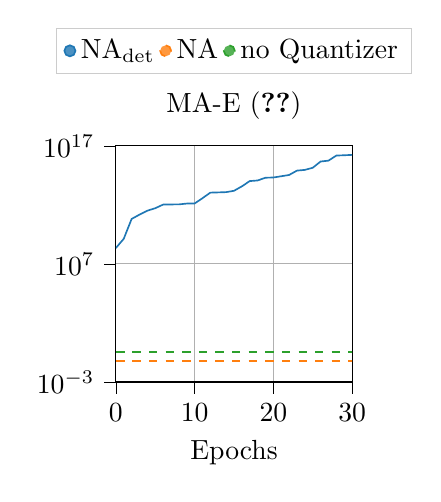
\begin{tikzpicture}

\definecolor{darkgray176}{RGB}{176,176,176}
\definecolor{darkorange25512714}{RGB}{255,127,14}
\definecolor{forestgreen4416044}{RGB}{44,160,44}
\definecolor{lightgray204}{RGB}{204,204,204}
\definecolor{steelblue31119180}{RGB}{31,119,180}

\begin{axis}[
         % Align it next to the first plot
    anchor=west,
    width=3cm,  % Adjust the width of the plot
    height=3cm, 
    legend cell align={center},
legend style={
  fill opacity=0.8,
  draw opacity=1,
  text opacity=1,
  at={(0.5,1.5)},
  anchor=north,
  draw=lightgray204,
  legend columns = -1
  mark=*
},
    legend image code/.code={
        \draw[mark options={scale=1}, mark=*] plot coordinates {(0.3cm,0cm)}; % Use points in the legend
    },
    % Adjust 
     xshift=1.5cm, %the height of the plot
    scale only axis, 
 title={MA-E (\ref{equ:MAE})},
log basis y={10},
tick align=outside,
tick pos=left,
x grid style={darkgray176},
xlabel={Epochs},
xmajorgrids,
xmin=0, xmax=30,
xtick style={color=black},
y grid style={darkgray176},
ymajorgrids,
ymin=0.001, ymax=10 0000000000000000,
ymode=log,
ytick style={color=black}
]
\addplot [semithick, steelblue31119180]
table {%
0 220920456.586761
1 1336126358.49353
2 63976024621.5685
3 148516052586.49
4 320987298775.846
5 517504113655.364
6 1051341255736.73
7 1081520208140.33
8 1093097830481.14
9 1277915579649.94
10 1303095408281.98
11 3659127229661.41
12 10826622393003.5
13 11293220986621
14 11914486941395.9
15 15450026732433.4
16 36711791912633.6
17 102606070269964
18 115514332066640
19 197521567035481
20 206259469442689
21 263319425419315
22 338359262263218
23 791294460225600
24 910537334295859
25 1.37393198631451e+15
26 4.65460455963129e+15
27 5.52125460382298e+15
28 1.48697738640337e+16
29 1.58119710192262e+16
30 1.69636369374388e+16
31 2.13666669903096e+16
};
\addlegendentry{$\text{NA}_{\text{det}}$}
\addplot [semithick, darkorange25512714, dashed]
table {%
0 0.0583785891631658
1 0.0583785891631658
2 0.0583785891631658
3 0.0583785891631658
4 0.0583785891631658
5 0.0583785891631658
6 0.0583785891631658
7 0.0583785891631658
8 0.0583785891631658
9 0.0583785891631658
10 0.0583785891631658
11 0.0583785891631658
12 0.0583785891631658
13 0.0583785891631658
14 0.0583785891631658
15 0.0583785891631658
16 0.0583785891631658
17 0.0583785891631658
18 0.0583785891631658
19 0.0583785891631658
20 0.0583785891631658
21 0.0583785891631658
22 0.0583785891631658
23 0.0583785891631658
24 0.0583785891631658
25 0.0583785891631658
26 0.0583785891631658
27 0.0583785891631658
28 0.0583785891631658
29 0.0583785891631658
30 0.0583785891631658
31 0.0583785891631658
};
\addlegendentry{NA}
\addplot [semithick, forestgreen4416044, dashed]
table {%
0 0.34256650745833
1 0.34256650745833
2 0.34256650745833
3 0.34256650745833
4 0.34256650745833
5 0.34256650745833
6 0.34256650745833
7 0.34256650745833
8 0.34256650745833
9 0.34256650745833
10 0.34256650745833
11 0.34256650745833
12 0.34256650745833
13 0.34256650745833
14 0.34256650745833
15 0.34256650745833
16 0.34256650745833
17 0.34256650745833
18 0.34256650745833
19 0.34256650745833
20 0.34256650745833
21 0.34256650745833
22 0.34256650745833
23 0.34256650745833
24 0.34256650745833
25 0.34256650745833
26 0.34256650745833
27 0.34256650745833
28 0.34256650745833
29 0.34256650745833
30 0.34256650745833
31 0.34256650745833
};
\addlegendentry{no Quantizer}
\end{axis}

\end{tikzpicture}

    \caption{Training \gls{MA-E} over epochs for an internal neural audio codec (trained on audio). The dashed lines are the final values of trained models. We show the evolvement over the epochs for $\text{NA}_\text{det}$. After $32$ epochs, the model training crashed as $E$ grew too large. The other two models were trained for more than $1000$ epochs.}
    \label{fig:xcodec}
\end{figure}
We repeat selected experiments with an internal audio codec and with \gls{DAC} trained using audio data to show the consistency of our findings. 


\textbf{Effect of NA on Internal Speech Codec}: First, we evaluate the effect of \gls{NA} when training an internal model for speech coding. The embedding norms are depicted in Figure~\ref{fig:xcodec}. When no quantizer or NA is used, the final \gls{MA-E} are in a similar range to the \gls{MA-E} of the low-complexity model in Figure~\ref{fig:enter-label} and Figure~\ref{fig:NIdetvsat}, respectively. When detaching the added noise in $\text{NA}_\text{det}$, $E$ keeps growing till the training crashes after approximately 30~epochs. This result is consistent with the growth of $E$ for the low complexity model in Figure~\ref{fig:NIdetvsat}. 

\textbf{Effect of STE/mSTE on Descript-Audio-Codec (DAC)}:
 \begin{figure}[t!]
    \centering
    % This file was created with tikzplotlib v0.10.1.
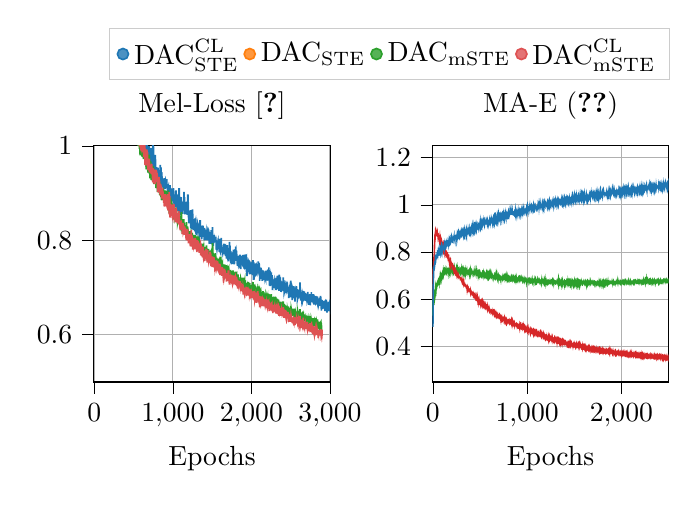
\begin{tikzpicture}

\definecolor{darkgray176}{RGB}{176,176,176}
\definecolor{darkorange25512714}{RGB}{255,127,14}
\definecolor{lightgray204}{RGB}{204,204,204}
\definecolor{steelblue31119180}{RGB}{31,119,180}
\definecolor{forestgreen4416044}{RGB}{44,160,44}
\definecolor{darkorange25512714}{RGB}{255,127,14}
\definecolor{crimson2143940}{RGB}{214,39,40}
\begin{axis}[
name = plot1,
    width=3cm,  % Adjust the width of the plot
    height=3cm,  % Adjust the height of the plot
    scale only axis, 
    xlabel={Epochs},
legend cell align={center},
legend style={
  fill opacity=0.8,
  draw opacity=1,
  text opacity=1,
  at={(1.25,1.5)},
  anchor=north,
  draw=lightgray204,
  legend columns = -1
  mark=*
},
legend image code/.code={
        \draw[mark options={scale=1}, mark=*] plot coordinates {(0.3cm,0cm)}; % Use points in the legend
    },
tick align=outside,
tick pos=left,
x grid style={darkgray176},
xmajorgrids,
xmin=-4.95, xmax=3001,
xtick style={color=black},
y grid style={darkgray176},
ylabel={},
title={Mel-Loss \cite{Kumar2023}},
ymajorgrids,
ymin=0.5, 
ymax=1,
ytick style={color=black},
]
\addplot [semithick, steelblue31119180]
table {%
0 3.8405385017395
1 3.2975513458252
2 3.01146774291992
3 2.87367647171021
4 2.71081328392029
5 2.62088143825531
6 2.54276392936707
7 2.50425898075104
8 2.39414689064026
9 2.35057700634003
10 2.32624480247498
11 2.24924365520477
12 2.22717481613159
13 2.20085351467133
14 2.18150094509125
15 2.12895694255829
16 2.11937940597534
17 2.07921057701111
18 2.08049725532532
19 2.05054449796677
20 2.05248263597488
21 2.03198372602463
22 1.9956635427475
23 1.977211997509
24 1.97663711547852
25 1.94388709306717
26 1.91995120286942
27 1.91661630153656
28 1.91253799915314
29 1.88886182546616
30 1.86216349363327
31 1.8688304066658
32 1.85537682056427
33 1.84764829158783
34 1.83636671543121
35 1.83130190372467
36 1.82241991281509
37 1.80730823755264
38 1.80091029405594
39 1.79263065576553
40 1.76952370882034
41 1.78002281427383
42 1.74235862731934
43 1.74293640851974
44 1.75227924346924
45 1.74536121845245
46 1.74547189712524
47 1.74021322965622
48 1.72981917858124
49 1.70166609525681
50 1.71485134124756
51 1.70884013652802
52 1.67722774982452
53 1.67327613830566
54 1.68437567710876
55 1.68736044883728
56 1.67188741922379
57 1.68666328430176
58 1.65546479701996
59 1.65111279249191
60 1.66048396348953
61 1.63677196741104
62 1.64883840560913
63 1.66325462579727
64 1.62456746578217
65 1.61648175001144
66 1.62725043773651
67 1.62506517410278
68 1.59376168251038
69 1.63344405412674
70 1.6025878572464
71 1.59379452228546
72 1.60191157341003
73 1.60921210050583
74 1.59103691577911
75 1.583158223629
76 1.59395758867264
77 1.55738127946854
78 1.57119514703751
79 1.58101963758469
80 1.55680814504623
81 1.54560365438461
82 1.56257195711136
83 1.54827023029327
84 1.52674243688583
85 1.54403115034103
86 1.55745791912079
87 1.52935580730438
88 1.5273260807991
89 1.54146965265274
90 1.54141367197037
91 1.51384971380234
92 1.53982813835144
93 1.5340755200386
94 1.50016462802887
95 1.51670392274857
96 1.51354923963547
97 1.51096559762955
98 1.49367137908936
99 1.51683893442154
100 1.49701533555985
101 1.51228804826736
102 1.49460859775543
103 1.49080303192139
104 1.49205719232559
105 1.46919034957886
106 1.46300401926041
107 1.47360087156296
108 1.47988039731979
109 1.45339062213898
110 1.47130946397781
111 1.4731062912941
112 1.4638871884346
113 1.46579273939133
114 1.46983590841293
115 1.45346446037292
116 1.45460157632828
117 1.44959918260574
118 1.44654527187347
119 1.4327557849884
120 1.43846100330353
121 1.44008057832718
122 1.43139693021774
123 1.42011606216431
124 1.44418730258942
125 1.42274734258652
126 1.42960076093674
127 1.43489737510681
128 1.43949997901916
129 1.4371866106987
130 1.42106143474579
131 1.4250098657608
132 1.41746160984039
133 1.3931513261795
134 1.4094553399086
135 1.4053119802475
136 1.39047882795334
137 1.38363596916199
138 1.40082840442657
139 1.3995694231987
140 1.39031559705734
141 1.41729611873627
142 1.41127730369568
143 1.39913031101227
144 1.40319042682648
145 1.414344394207
146 1.41047002077103
147 1.39192660808563
148 1.39572037220001
149 1.3894313955307
150 1.37863300323486
151 1.38301538944244
152 1.38297313451767
153 1.3691602897644
154 1.35944576025009
155 1.35659193515778
156 1.3602428817749
157 1.3519966673851
158 1.3666277551651
159 1.35426378965378
160 1.35904506206512
161 1.36404261827469
162 1.38160753965378
163 1.39164017915726
164 1.36503009080887
165 1.37146654367447
166 1.35913357257843
167 1.37172684431076
168 1.33367505073547
169 1.34766741275787
170 1.33312819719315
171 1.32021584510803
172 1.3088271188736
173 1.31783190488815
174 1.31406824827194
175 1.30727591276169
176 1.30937158346176
177 1.3116219496727
178 1.32800549507141
179 1.32637124538422
180 1.34508996486664
181 1.33230921030045
182 1.35461894273758
183 1.35012014627457
184 1.35317333459854
185 1.35888725996017
186 1.34173710346222
187 1.31883167505264
188 1.31086048126221
189 1.32512051582336
190 1.31112251520157
191 1.29607800722122
192 1.29104441165924
193 1.31182778835297
194 1.2895151758194
195 1.28287826776505
196 1.29981463670731
197 1.30365651607513
198 1.28857781887054
199 1.28901496887207
200 1.32185843229294
201 1.30960609674454
202 1.3030172586441
203 1.29443945646286
204 1.33027235507965
205 1.3104680109024
206 1.3187485408783
207 1.31141619205475
208 1.30082471847534
209 1.29382658720016
210 1.27354792356491
211 1.29521421909332
212 1.27817254066467
213 1.27942135095596
214 1.26712846279144
215 1.26745729207993
216 1.27934220790863
217 1.28049825906754
218 1.28235827922821
219 1.29488910198212
220 1.28975210905075
221 1.2742956161499
222 1.29616009473801
223 1.31287279844284
224 1.28407236099243
225 1.28260902166367
226 1.30205222129822
227 1.30024926424026
228 1.27056899547577
229 1.2785945057869
230 1.28635031700134
231 1.27280110359192
232 1.26444640874863
233 1.26535922527313
234 1.29191809415817
235 1.25514150619507
236 1.26097883224487
237 1.27535816431046
238 1.28944331645966
239 1.25338122606277
240 1.25761610507965
241 1.28230465888977
242 1.2631179523468
243 1.25220862150192
244 1.24419703006744
245 1.26319929361343
246 1.24106340885162
247 1.25165003299713
248 1.24359050512314
249 1.24049252748489
250 1.2428249835968
251 1.22076571941376
252 1.2429452753067
253 1.23860658407211
254 1.23146056175232
255 1.2295544219017
256 1.24141356229782
257 1.24595829963684
258 1.24568543195724
259 1.25876354694366
260 1.25768580675125
261 1.24501749038696
262 1.24312579631805
263 1.257229180336
264 1.23856081485748
265 1.22976551771164
266 1.21366612911224
267 1.23789676189423
268 1.21569811582565
269 1.19102829694748
270 1.22116300106049
271 1.22567471265793
272 1.21377497911453
273 1.19979765415192
274 1.23053088188171
275 1.23692737340927
276 1.21988799095154
277 1.22194601774216
278 1.23586396694183
279 1.23933170318604
280 1.22936749458313
281 1.2383061170578
282 1.23293946027756
283 1.21774699211121
284 1.2253463768959
285 1.21742326021194
286 1.21914077997208
287 1.18495881795883
288 1.216840467453
289 1.20112912893295
290 1.1923456454277
291 1.20424015522003
292 1.19681729793549
293 1.20328501224518
294 1.18537227153778
295 1.2102640080452
296 1.19391227960587
297 1.19731403827667
298 1.19023005723953
299 1.20242822885513
300 1.19505621194839
301 1.20316512584686
302 1.213932492733
303 1.20080914735794
304 1.2063804936409
305 1.19385503768921
306 1.22224251508713
307 1.19481440067291
308 1.20500308990479
309 1.20331734418869
310 1.19950291633606
311 1.18809916257858
312 1.19478008508682
313 1.20182383060455
314 1.17786189317703
315 1.18930806159973
316 1.1822370672226
317 1.1847291636467
318 1.17078946828842
319 1.1945138001442
320 1.17458564281464
321 1.16665298461914
322 1.16286026954651
323 1.17312188625336
324 1.17626168251038
325 1.16383533239365
326 1.18074680805206
327 1.17066483020782
328 1.17111032962799
329 1.16941276550293
330 1.19220526695251
331 1.17136203527451
332 1.17813742876053
333 1.18328507661819
334 1.17627420425415
335 1.17409434318542
336 1.16227745294571
337 1.17907240867615
338 1.16596975564957
339 1.17640712976456
340 1.16705902814865
341 1.15850468873978
342 1.15718527078629
343 1.16553797245026
344 1.16971768856049
345 1.14549443244934
346 1.15914708852768
347 1.16089956283569
348 1.17464614629745
349 1.14389717102051
350 1.17448381662369
351 1.17135594844818
352 1.16808860301971
353 1.1528547668457
354 1.17748000144958
355 1.16846626758575
356 1.13052346467972
357 1.16377373456955
358 1.15018020391464
359 1.15029183387756
360 1.12700267076492
361 1.17624351024628
362 1.13825152397156
363 1.14573605179787
364 1.12787302732468
365 1.1740702009201
366 1.15022631406784
367 1.13618708848953
368 1.14865471601486
369 1.15010756969452
370 1.14972007989883
371 1.13945575237274
372 1.16678467273712
373 1.12744161844254
374 1.15010075330734
375 1.13834487915039
376 1.16863394737244
377 1.12822947978973
378 1.1509001660347
379 1.15226058006287
380 1.14611324310303
381 1.15470249891281
382 1.14897245883942
383 1.17247111558914
384 1.12620388031006
385 1.1517739033699
386 1.14033972263336
387 1.16053770065308
388 1.11150177121162
389 1.13577464103699
390 1.13490390300751
391 1.13871850252151
392 1.10753590703011
393 1.13152362108231
394 1.14788918972015
395 1.11749869823456
396 1.1283615732193
397 1.14457275867462
398 1.15660738706589
399 1.11229697704315
400 1.13911200284958
401 1.16973579406738
402 1.14370458126068
403 1.11314159154892
404 1.16244823694229
405 1.16907079935074
406 1.11741590976715
407 1.12969089031219
408 1.15237653017044
409 1.1429790019989
410 1.10024678707123
411 1.12729561090469
412 1.1318425154686
413 1.10182076334953
414 1.10002063035965
415 1.12590431213379
416 1.11278753757477
417 1.08738144755363
418 1.10629148721695
419 1.11189222574234
420 1.08706076383591
421 1.07555535435677
422 1.11772082328796
423 1.09783133506775
424 1.08665708065033
425 1.10147181749344
426 1.12336714744568
427 1.10431660652161
428 1.09243436336517
429 1.13996119260788
430 1.10658819437027
431 1.10909628152847
432 1.11656410694122
433 1.16331671714783
434 1.10532874584198
435 1.10944717645645
436 1.12079589128494
437 1.12287993907928
438 1.08813195943832
439 1.09650781273842
440 1.13165456295013
441 1.08978409290314
442 1.08344819068909
443 1.09677150726318
444 1.10928888320923
445 1.0835000371933
446 1.0894244992733
447 1.09991306781769
448 1.09609416484833
449 1.07445851564407
450 1.09225004673004
451 1.09479867219925
452 1.08151543855667
453 1.08232951760292
454 1.08507094860077
455 1.10561996459961
456 1.08095949888229
457 1.08751544952393
458 1.08721635341644
459 1.09170059919357
460 1.07942420482635
461 1.08889036655426
462 1.09178212165833
463 1.09084659814835
464 1.08768829107285
465 1.08200062990189
466 1.0921416425705
467 1.08603340029716
468 1.09166906118393
469 1.08019224643707
470 1.09414308786392
471 1.08408058166504
472 1.07751049280167
473 1.09602051496506
474 1.08092482328415
475 1.08001728415489
476 1.07034325838089
477 1.08636236667633
478 1.08411050081253
479 1.07872761964798
480 1.0745135140419
481 1.09846110105515
482 1.07697755932808
483 1.0649017739296
484 1.08381256341934
485 1.08173844337463
486 1.07725960493088
487 1.05854099273682
488 1.09131686925888
489 1.08842861533165
490 1.0671768784523
491 1.06902590274811
492 1.11400272607803
493 1.08894967675209
494 1.06361714601517
495 1.09837940454483
496 1.13114570498466
497 1.07552610516548
498 1.07029231071472
499 1.14392886400223
500 1.08943986177444
501 1.06622446775436
502 1.071645424366
503 1.10939756274223
504 1.0577102804184
505 1.04778288006783
506 1.07412004709244
507 1.05977254867554
508 1.03248467445374
509 1.04262420892715
510 1.05889722824097
511 1.04001271009445
512 1.0268897652626
513 1.03506222844124
514 1.03267450213432
515 1.03191840410233
516 1.02298105359077
517 1.03042057156563
518 1.03001174807549
519 1.02058461308479
520 1.03291454672813
521 1.04131013393402
522 1.03868086099625
523 1.02761126875877
524 1.04126530766487
525 1.05380382418633
526 1.04465599894524
527 1.04381709694862
528 1.08875964403152
529 1.07275593042374
530 1.06025861859322
531 1.07966855764389
532 1.12342591047287
533 1.05989813327789
534 1.05816830158234
535 1.07637581348419
536 1.03847970962524
537 1.03958935260773
538 1.03383003592491
539 1.04765007615089
540 1.03160576701164
541 1.03254517436028
542 1.03665862560272
543 1.02393432974815
544 1.02211881995201
545 1.02603647232056
546 1.01809185862541
547 1.00379648447037
548 1.01937366962433
549 1.02228921294212
550 1.01945448160172
551 1.02674987196922
552 1.02361059427261
553 1.0346221601963
554 1.02932510852814
555 1.03170567989349
556 1.04169640541077
557 1.04904188156128
558 1.0383049929142
559 1.04324440002441
560 1.05386678695679
561 1.04621523737907
562 1.0338925755024
563 1.0498300242424
564 1.03265678405762
565 1.04036995053291
566 1.02883964419365
567 1.03267513036728
568 1.02428009390831
569 1.01738684773445
570 1.0203399348259
571 1.02612041473389
572 1.02159067153931
573 1.01591320753098
574 1.01355197310448
575 1.01711947321892
576 1.01566284298897
577 1.00800785303116
578 1.01325110197067
579 1.03185002207756
580 1.01020372271538
581 1.01423902392387
582 1.03390022039413
583 1.02264416217804
584 1.02557238936424
585 1.02172681331635
586 1.04715457201004
587 1.02301898241043
588 1.03188203334808
589 1.03942478299141
590 1.03335252761841
591 1.03453310489655
592 1.03364817976952
593 1.03868736982346
594 1.01683166265488
595 1.00914742946625
596 1.01765400409698
597 1.02919790029526
598 1.01318461179733
599 1.00771780371666
600 1.01272418498993
601 1.01060293912888
602 1.00408141732216
603 1.00710309624672
604 1.01738147139549
605 1.01448585987091
606 1.00120688319206
607 1.00314438462257
608 1.02769908070564
609 1.01324047088623
610 0.999308584928513
611 1.02266116142273
612 1.02915570020676
613 1.01806723833084
614 1.01396467924118
615 1.03049938678741
616 1.01424492478371
617 1.0109682059288
618 1.01540071964264
619 1.02342773795128
620 1.00948843359947
621 0.996241550445557
622 1.02161776185036
623 1.00642395853996
624 1.00184969186783
625 1.00811475992203
626 1.00368576407433
627 0.989481798410416
628 0.994613436460495
629 1.00177989125252
630 0.994710586071014
631 1.00031599521637
632 0.995373078584671
633 1.01658559799194
634 0.987606173753738
635 1.00714328050613
636 1.00726819753647
637 1.01328750491142
638 1.00152953863144
639 1.00572978138924
640 1.01463999867439
641 1.00773760557175
642 1.00698269486427
643 1.00201040148735
644 1.01391112923622
645 0.996095370054245
646 1.01051591038704
647 0.99045747756958
648 1.00187915802002
649 0.999140664339066
650 0.994697107076645
651 1.00054263830185
652 0.995914188623428
653 1.0058635020256
654 0.988192347288132
655 0.994011189937592
656 1.00412021279335
657 0.993958603143692
658 0.992934664487839
659 1.00960588097572
660 1.00060281395912
661 0.985151754617691
662 1.00091777443886
663 1.01218108892441
664 0.996934251785278
665 0.981450299024582
666 1.00349858045578
667 0.988125296831131
668 0.99153706073761
669 0.988760845661163
670 0.992827161550522
671 0.983382052183151
672 0.993850206136703
673 0.988180893659592
674 0.985923273563385
675 1.00297911167145
676 0.988843973875046
677 0.989002383947372
678 0.987655568122864
679 0.99179062128067
680 0.991563524007797
681 0.980480070114136
682 0.973024454116821
683 0.98382082939148
684 0.975890048742294
685 0.977616981267929
686 0.973525009155273
687 0.980054305791855
688 0.97689972281456
689 0.981650770902634
690 0.977638714313507
691 0.978862783908844
692 0.979088830947876
693 0.974957809448242
694 0.970047351121902
695 0.989785143136978
696 0.980944662094116
697 0.981686253547668
698 0.988704100847244
699 0.999013221263885
700 0.9797702729702
701 0.962875282764435
702 0.985974509716034
703 0.981389677524567
704 0.967214223146439
705 0.976187626123428
706 0.979719371795654
707 0.975342737436295
708 0.965416656732559
709 0.971529763936996
710 0.982042719125748
711 0.971903858184815
712 0.965306550264359
713 0.989044232368469
714 0.987820528745651
715 0.972819520235062
716 0.971515743732452
717 0.995089073181152
718 0.987078924179077
719 0.972232208251953
720 0.978289395570755
721 0.992052093744278
722 0.978147133588791
723 0.971608725786209
724 0.975825802087784
725 0.986056312322617
726 0.964470999240875
727 0.978085536956787
728 0.983902815580368
729 0.995112165212631
730 0.964431354999542
731 0.972823268175125
732 0.991724421977997
733 0.964879096746445
734 0.954745936393738
735 0.97168221950531
736 0.986154894828796
737 0.951374452114105
738 0.97014577627182
739 0.988769096136093
740 0.977809292078018
741 0.960768146514893
742 0.964298249483108
743 1.02116020202637
744 0.962621788978577
745 0.949826608896255
746 0.984619289636612
747 1.00230448007584
748 0.939494128227234
749 0.962347700595856
750 0.995017778873444
751 0.977908481359482
752 0.939817509651184
753 0.957559188604355
754 0.998908017873764
755 0.942795442342758
756 0.932825446128845
757 0.964716606140137
758 0.978571799993515
759 0.935419670343399
760 0.942823457717896
761 0.953241016864777
762 0.964785702228546
763 0.932335424423218
764 0.943252286911011
765 0.967940247058868
766 0.941332856416702
767 0.942787212133408
768 0.952547365427017
769 0.973109441995621
770 0.944884238243103
771 0.954631569385529
772 0.96674818277359
773 0.962502375841141
774 0.955863053798676
775 0.95762011885643
776 0.980785368680954
777 0.954522479772568
778 0.947671848535538
779 0.949054330587387
780 0.97141324877739
781 0.938464077711105
782 0.947740856409073
783 0.954876259565353
784 0.945534596443176
785 0.936086709499359
786 0.950512365102768
787 0.95477338552475
788 0.935014771223068
789 0.936824268102646
790 0.941450426578522
791 0.940215598344803
792 0.93371674656868
793 0.947620633840561
794 0.942161011695862
795 0.940123487710953
796 0.946432287693024
797 0.946097692251205
798 0.94139564871788
799 0.94360358953476
800 0.954439569711685
801 0.94010236620903
802 0.946403130292892
803 0.948298214673996
804 0.95110579252243
805 0.937821009159088
806 0.934940272569656
807 0.944445097446442
808 0.93467817902565
809 0.93940535068512
810 0.945669434070587
811 0.952483787536621
812 0.938576807975769
813 0.950439208745956
814 0.942313673496246
815 0.943204627037048
816 0.941609282493591
817 0.939684207439423
818 0.949045912027359
819 0.934936162233353
820 0.943579050302505
821 0.93972668170929
822 0.944115650653839
823 0.932446043491364
824 0.944426765441895
825 0.938668677806854
826 0.941695837974548
827 0.922153089046478
828 0.937464234828949
829 0.941942231655121
830 0.933048745393753
831 0.927857716083527
832 0.943768846988678
833 0.928880962133408
834 0.920717477798462
835 0.928571348190308
836 0.93671725153923
837 0.93443208694458
838 0.915163387060165
839 0.934175561666489
840 0.959417439699173
841 0.92938129067421
842 0.920365962982178
843 0.928903722763062
844 0.940636968612671
845 0.919224834442139
846 0.9273950278759
847 0.949520123004913
848 0.942277339696884
849 0.915041579008102
850 0.9222842669487
851 0.954452718496323
852 0.936520725488663
853 0.923626606464386
854 0.940599752664566
855 0.937327765226364
856 0.919095964431763
857 0.932882735729218
858 0.944327456951141
859 0.939705047607422
860 0.930302050113678
861 0.927219127416611
862 0.933925403356552
863 0.920270134210587
864 0.935267617702484
865 0.923369929790497
866 0.927994511127472
867 0.928040524721146
868 0.915724686384201
869 0.921711058616638
870 0.929423022270203
871 0.926355422735214
872 0.915748748779297
873 0.919903687238693
874 0.918113609552383
875 0.925137476921082
876 0.911733241081238
877 0.929219975471497
878 0.923628526926041
879 0.910666645765305
880 0.915146563053131
881 0.922295653820038
882 0.923617876768112
883 0.907140667438507
884 0.921046581268311
885 0.916991591453552
886 0.918907129764557
887 0.920366566181183
888 0.925451718568802
889 0.925529370307922
890 0.920528696775436
891 0.930829360485077
892 0.910201900005341
893 0.931484681367874
894 0.921302065849304
895 0.920074956417084
896 0.918023399114609
897 0.908283243179321
898 0.914042323827744
899 0.914237197637558
900 0.926311798095703
901 0.912165702581406
902 0.92126411318779
903 0.917658809423447
904 0.908616080284119
905 0.91564885020256
906 0.920054025650024
907 0.911311837434769
908 0.915302480459213
909 0.925186032056808
910 0.928018058538437
911 0.918145571947098
912 0.910724629163742
913 0.925153778791428
914 0.924608691930771
915 0.917830276489258
916 0.923295325040817
917 0.920956872701645
918 0.912199863195419
919 0.914552509784698
920 0.919739421606064
921 0.913672549724579
922 0.915279716253281
923 0.91696266412735
924 0.929271188974381
925 0.91769926905632
926 0.913547316789627
927 0.918882712125778
928 0.912832858562469
929 0.914633976221085
930 0.916697969436645
931 0.9120370221138
932 0.903956604003906
933 0.90670118689537
934 0.91116309762001
935 0.907970716953278
936 0.90977218747139
937 0.894966524839401
938 0.902872167825699
939 0.913288977146149
940 0.903302298784256
941 0.908644148111343
942 0.911908798217773
943 0.912531319856644
944 0.907772974967957
945 0.907272864580154
946 0.90521414399147
947 0.915515165328979
948 0.90471059679985
949 0.904384876489639
950 0.908368344306946
951 0.901467282772064
952 0.898808709383011
953 0.883302968740463
954 0.916055272817612
955 0.904928456544876
956 0.890952625274658
957 0.902946150302887
958 0.904438390731812
959 0.896254394054413
960 0.899640692472458
961 0.907942779064178
962 0.91519829750061
963 0.916753826141357
964 0.898946793079376
965 0.916628897190094
966 0.901006869077682
967 0.911451970338821
968 0.896814445257187
969 0.898627897500992
970 0.908370065689087
971 0.896408232450485
972 0.897884172201157
973 0.884780300855637
974 0.900709369182587
975 0.904286524057388
976 0.893714587688446
977 0.899257062673569
978 0.903996013402939
979 0.893328058719635
980 0.892541506290436
981 0.90973507642746
982 0.893357707262039
983 0.890752305984497
984 0.894118514060974
985 0.905968047380447
986 0.900340673923492
987 0.895350058078766
988 0.89313374876976
989 0.897718091011047
990 0.904181917905807
991 0.883138378858566
992 0.898169875144958
993 0.907726333141327
994 0.892040761709213
995 0.892884291410446
996 0.894592247009277
997 0.900661256313324
998 0.89251572728157
999 0.890950537919998
1000 0.896434738636017
1001 0.900868583917618
1002 0.887559653520584
1003 0.900920159816742
1004 0.908534076213837
1005 0.895609191656113
1006 0.901791818141937
1007 0.90692755818367
1008 0.910089933872223
1009 0.887468023300171
1010 0.900715264081955
1011 0.903610343933105
1012 0.892360055446625
1013 0.896806553602219
1014 0.896930578947067
1015 0.890193046331406
1016 0.877559615373611
1017 0.887360739707947
1018 0.880722578763962
1019 0.883139916658402
1020 0.873398180007935
1021 0.878372093439102
1022 0.879506978988647
1023 0.872124297618866
1024 0.881586155891418
1025 0.873155217170715
1026 0.881408377885818
1027 0.870630635023117
1028 0.886796585321426
1029 0.873428475856781
1030 0.878151100873947
1031 0.886791167259216
1032 0.870855919122696
1033 0.876161997318268
1034 0.883448324203491
1035 0.894623411893845
1036 0.882622684240341
1037 0.889533303976059
1038 0.893397034406662
1039 0.889560700654983
1040 0.881694411039352
1041 0.905484280586243
1042 0.894315366744995
1043 0.876542639732361
1044 0.899449836015701
1045 0.889169983863831
1046 0.894171843528748
1047 0.880173748731613
1048 0.896965303421021
1049 0.887401162385941
1050 0.889414007663727
1051 0.871713932752609
1052 0.897644573450089
1053 0.882353016138077
1054 0.869347593784332
1055 0.879880896806717
1056 0.883030304908752
1057 0.881182036399841
1058 0.865337560176849
1059 0.878281590938568
1060 0.878597594499588
1061 0.870772590637207
1062 0.876934770345688
1063 0.878955253362656
1064 0.873200739622116
1065 0.861651427745819
1066 0.88160459280014
1067 0.886602494716644
1068 0.873074252605438
1069 0.867784209251404
1070 0.887123239040375
1071 0.878459718227386
1072 0.861143891811371
1073 0.87863698720932
1074 0.879693033695221
1075 0.890833325386047
1076 0.875000019073486
1077 0.910164344310761
1078 0.88654762506485
1079 0.882288062572479
1080 0.893967459201813
1081 0.910254592895508
1082 0.878034045696259
1083 0.879161952733994
1084 0.884359413385391
1085 0.892979502677917
1086 0.870026634931564
1087 0.861203374862671
1088 0.875327037572861
1089 0.873516660928726
1090 0.856718322038651
1091 0.856524776220322
1092 0.872398506402969
1093 0.868843965530396
1094 0.856554042100906
1095 0.856435703039169
1096 0.873398131132126
1097 0.855298557281494
1098 0.85770751953125
1099 0.861601836681366
1100 0.856021128892899
1101 0.857457375526428
1102 0.867191284894943
1103 0.86620815038681
1104 0.862302277088165
1105 0.858924868106842
1106 0.87105718255043
1107 0.869057040214539
1108 0.866925324201584
1109 0.891311342716217
1110 0.870084216594696
1111 0.87811271905899
1112 0.875735419988632
1113 0.880819615125656
1114 0.877696509361267
1115 0.865612503290176
1116 0.873988741636276
1117 0.876797207593918
1118 0.867550175189972
1119 0.870264099836349
1120 0.879850165843964
1121 0.857140871286392
1122 0.864463211297989
1123 0.8616921210289
1124 0.879441921710968
1125 0.861262776851654
1126 0.855725929737091
1127 0.868094388246536
1128 0.858641088008881
1129 0.866574152708054
1130 0.867482123374939
1131 0.87502394080162
1132 0.867287704944611
1133 0.86266030550003
1134 0.874973719120026
1135 0.875862542390823
1136 0.870145661830902
1137 0.869100506305695
1138 0.883936401605606
1139 0.876016561985016
1140 0.865814900398254
1141 0.873361706733704
1142 0.902335035800934
1143 0.867973897457123
1144 0.8704410135746
1145 0.885368672609329
1146 0.879579178094864
1147 0.870847572088242
1148 0.864613901376724
1149 0.891080815792084
1150 0.866295602321625
1151 0.863771132230759
1152 0.867613285779953
1153 0.875002263784409
1154 0.865807312726975
1155 0.855099859237671
1156 0.867438004016876
1157 0.86578693151474
1158 0.870563920736313
1159 0.857678980827332
1160 0.867199240922928
1161 0.861414946317673
1162 0.865945000648499
1163 0.859395995140076
1164 0.857485758066177
1165 0.881292159557343
1166 0.864348614215851
1167 0.859307050704956
1168 0.864716957807541
1169 0.872744990587235
1170 0.866654196977615
1171 0.86675986289978
1172 0.868222033977509
1173 0.872007219791412
1174 0.880258837938309
1175 0.876959210634232
1176 0.876656626462936
1177 0.858596960306168
1178 0.865328197479248
1179 0.868554904460907
1180 0.869085993766785
1181 0.85552023768425
1182 0.875492407083511
1183 0.880350600481033
1184 0.853705347776413
1185 0.859560644626617
1186 0.882696088552475
1187 0.868162696361542
1188 0.860688372850418
1189 0.876586517095566
1190 0.897016032934189
1191 0.878333506584168
1192 0.865687537193298
1193 0.896612775325775
1194 0.878899154663086
1195 0.859671015739441
1196 0.871806998252869
1197 0.880723176002502
1198 0.858087283372879
1199 0.848396220207214
1200 0.862103189229965
1201 0.854163262844086
1202 0.83978355884552
1203 0.841022462844849
1204 0.856282526254654
1205 0.845719895362854
1206 0.846202427148819
1207 0.841685866117477
1208 0.851789101362228
1209 0.840393333435059
1210 0.838685382604599
1211 0.844509420394898
1212 0.849160906076431
1213 0.835784367322922
1214 0.851136828660965
1215 0.846914327144623
1216 0.846106848716736
1217 0.845961804389954
1218 0.854377553462982
1219 0.861493864059448
1220 0.845841197967529
1221 0.845173655748367
1222 0.861047775745392
1223 0.847071485519409
1224 0.842739306688309
1225 0.85806388258934
1226 0.863544565439224
1227 0.833854709863663
1228 0.827420433759689
1229 0.849252150058746
1230 0.842237932682037
1231 0.826059905290604
1232 0.839859457015991
1233 0.841703679561615
1234 0.826507904529572
1235 0.84182596206665
1236 0.843461052179337
1237 0.838577595949173
1238 0.826806634664536
1239 0.823068298101425
1240 0.834783923625946
1241 0.825821975469589
1242 0.83324568271637
1243 0.834048074483871
1244 0.847743471860886
1245 0.833035997152328
1246 0.840864206552505
1247 0.850116407871246
1248 0.860884144306183
1249 0.839987764358521
1250 0.853189644813538
1251 0.865165399312973
1252 0.839150506258011
1253 0.856018426418304
1254 0.843027189970016
1255 0.853021658658981
1256 0.84222495675087
1257 0.836915180683136
1258 0.83634471654892
1259 0.832337431907654
1260 0.836275857686996
1261 0.829913492202759
1262 0.825911940336227
1263 0.821505534648895
1264 0.836936959028244
1265 0.833740755319595
1266 0.82588564157486
1267 0.825551962852478
1268 0.839232702255249
1269 0.832417699098587
1270 0.832439737319946
1271 0.824027849435806
1272 0.836314424276352
1273 0.827849975824356
1274 0.826766359806061
1275 0.838862404823303
1276 0.827465343475342
1277 0.824855843782425
1278 0.824311269521713
1279 0.839995871782303
1280 0.83228408575058
1281 0.827856557369232
1282 0.846062695980072
1283 0.837546451091766
1284 0.833702300786972
1285 0.83015496969223
1286 0.838131759166718
1287 0.838860725164413
1288 0.831670875549316
1289 0.821749452352524
1290 0.845209975242615
1291 0.826898950338364
1292 0.830390141010284
1293 0.817566312551498
1294 0.830014799833298
1295 0.824533498287201
1296 0.825044727325439
1297 0.823904368877411
1298 0.818381781578064
1299 0.827050399780273
1300 0.817573224306107
1301 0.825978871583939
1302 0.810699373483658
1303 0.821133592128754
1304 0.822058855295181
1305 0.823796256780624
1306 0.810317140817642
1307 0.822148711681366
1308 0.832241306304932
1309 0.822218782901764
1310 0.823382842540741
1311 0.826125477552414
1312 0.828772020339966
1313 0.816135165691376
1314 0.825901948213577
1315 0.836852637529373
1316 0.83625089764595
1317 0.819923268556595
1318 0.831665291786194
1319 0.827593837976456
1320 0.817895419597626
1321 0.820233207941055
1322 0.830093930959702
1323 0.834787527322769
1324 0.814865555763245
1325 0.8257634973526
1326 0.823366785049438
1327 0.822905402183533
1328 0.819060406684875
1329 0.827427291870117
1330 0.835465890169144
1331 0.826286418437958
1332 0.82341078042984
1333 0.823319747447968
1334 0.835207220315933
1335 0.802857649326324
1336 0.819149469137192
1337 0.823995225429535
1338 0.822138960361481
1339 0.81557199716568
1340 0.824494886398315
1341 0.83144419670105
1342 0.810993928909302
1343 0.822927432060242
1344 0.826410762071609
1345 0.842635549306869
1346 0.820212494134903
1347 0.825299292802811
1348 0.842504065036774
1349 0.819757981300354
1350 0.824824556112289
1351 0.828170249462128
1352 0.831235973834991
1353 0.808414912223816
1354 0.822842762470245
1355 0.821268445253372
1356 0.807038421630859
1357 0.821206591129303
1358 0.820389490127563
1359 0.823516499996185
1360 0.809358515739441
1361 0.81904058098793
1362 0.811615047454834
1363 0.807871981859207
1364 0.804580634832382
1365 0.816945903301239
1366 0.825418870449066
1367 0.802069684267044
1368 0.81622708439827
1369 0.820877746343613
1370 0.826443686485291
1371 0.808359642028809
1372 0.81864771604538
1373 0.830813748836517
1374 0.810020374059677
1375 0.812000433206558
1376 0.83008580327034
1377 0.822987878322601
1378 0.807080838680267
1379 0.827345706224441
1380 0.830955853462219
1381 0.820708199739456
1382 0.811123229265213
1383 0.827580854892731
1384 0.831191892623901
1385 0.807037402391434
1386 0.811915392875671
1387 0.814781121015549
1388 0.813694732189178
1389 0.809828218221664
1390 0.81313503742218
1391 0.811156311035156
1392 0.819502931833267
1393 0.815989042520523
1394 0.822575058937073
1395 0.816783540248871
1396 0.811116416454315
1397 0.823216257095337
1398 0.813584522008896
1399 0.813934698104858
1400 0.801117709875107
1401 0.813390507698059
1402 0.814334279298782
1403 0.79988636136055
1404 0.822242383956909
1405 0.826298624277115
1406 0.813770629167557
1407 0.817350130081177
1408 0.819776000976562
1409 0.812542191743851
1410 0.808918069601059
1411 0.812326326370239
1412 0.81355543255806
1413 0.814648362398148
1414 0.800562254190445
1415 0.812642885446549
1416 0.822608501911163
1417 0.808468129634857
1418 0.811066325902939
1419 0.816253584623337
1420 0.81646111369133
1421 0.812749854326248
1422 0.816077411174774
1423 0.820777292251587
1424 0.81354761838913
1425 0.812905389070511
1426 0.819414844512939
1427 0.821418064832687
1428 0.808976148366928
1429 0.816482788324356
1430 0.814172625541687
1431 0.811367131471634
1432 0.811662700176239
1433 0.813891829252243
1434 0.816230478286743
1435 0.802268614768982
1436 0.817868067026138
1437 0.8170439016819
1438 0.814798221588135
1439 0.799958120584488
1440 0.816616870164871
1441 0.821572203636169
1442 0.808168054819107
1443 0.816309732198715
1444 0.817648123502731
1445 0.825345032215118
1446 0.811739448308945
1447 0.8102627825737
1448 0.821525675058365
1449 0.812316417694092
1450 0.81755450963974
1451 0.818232457637787
1452 0.817640433311462
1453 0.822058311700821
1454 0.821680521965027
1455 0.808241310119629
1456 0.802456923723221
1457 0.812801795005798
1458 0.819773807525635
1459 0.803230886459351
1460 0.800044051408768
1461 0.815184308290482
1462 0.793057441711426
1463 0.795102103948593
1464 0.800136433839798
1465 0.80866329908371
1466 0.79265240073204
1467 0.793940433263779
1468 0.804549454450607
1469 0.79943855047226
1470 0.79540314912796
1471 0.794178708791733
1472 0.801049554347992
1473 0.807875547409058
1474 0.798216588497162
1475 0.808139626979828
1476 0.817224481105804
1477 0.803007318973541
1478 0.802615545988083
1479 0.807488890886307
1480 0.812566118240356
1481 0.807279148101807
1482 0.80220903635025
1483 0.811812504529953
1484 0.812799441814423
1485 0.814976066350937
1486 0.792467424869537
1487 0.821273235082626
1488 0.807308800220489
1489 0.805383685827255
1490 0.808355244398117
1491 0.80528174161911
1492 0.808571754693985
1493 0.792626057863235
1494 0.812416085004807
1495 0.809193861484528
1496 0.800666406154633
1497 0.799997913837433
1498 0.814174972772598
1499 0.817023240327835
1500 0.798608245849609
1501 0.802119389772415
1502 0.812659854888916
1503 0.804842383861542
1504 0.790331437587738
1505 0.827786310911179
1506 0.805352358818054
1507 0.804449644088745
1508 0.811316548585892
1509 0.810972498655319
1510 0.80522225022316
1511 0.791458126306534
1512 0.8051194024086
1513 0.795853050947189
1514 0.795573056936264
1515 0.787602429389954
1516 0.798493782281876
1517 0.794832825660706
1518 0.79922758102417
1519 0.794780253171921
1520 0.801454728841782
1521 0.803617149591446
1522 0.793878653049469
1523 0.803443360328674
1524 0.797134557962418
1525 0.79829005241394
1526 0.795882451534271
1527 0.810638452768326
1528 0.806979546546936
1529 0.797506763935089
1530 0.799489839076996
1531 0.806465051174164
1532 0.806432538032532
1533 0.801509131193161
1534 0.797544556856155
1535 0.798673924207687
1536 0.802447611093521
1537 0.795449786186218
1538 0.80391659617424
1539 0.805035132169724
1540 0.799723913669586
1541 0.801881079673767
1542 0.796888060569763
1543 0.803486657142639
1544 0.796917983293533
1545 0.79843689084053
1546 0.806522789001465
1547 0.803301470279694
1548 0.799834101200104
1549 0.796600422859192
1550 0.798317189216614
1551 0.792489234209061
1552 0.793182724714279
1553 0.795190663337707
1554 0.793997638225555
1555 0.786862779855728
1556 0.782961835861206
1557 0.79222683429718
1558 0.780639448165894
1559 0.791339076757431
1560 0.786156417131424
1561 0.782236731052399
1562 0.780857175588608
1563 0.781955922842026
1564 0.791206711530685
1565 0.781598212718964
1566 0.786293567419052
1567 0.78755051612854
1568 0.785305699110031
1569 0.787644432783127
1570 0.787848724126816
1571 0.79945165514946
1572 0.786401818990707
1573 0.79561337351799
1574 0.791851632595062
1575 0.797869083881378
1576 0.798695459365845
1577 0.796603639125824
1578 0.798508044481277
1579 0.803299548625946
1580 0.792150186300278
1581 0.790851242542267
1582 0.789546089172363
1583 0.799018065929413
1584 0.803666695356369
1585 0.781333328485489
1586 0.795424134731293
1587 0.793028248548508
1588 0.789590026140213
1589 0.778740252256393
1590 0.782272695302963
1591 0.779617224931717
1592 0.775466012954712
1593 0.777559326887131
1594 0.784396994113922
1595 0.780133794546127
1596 0.792777626514435
1597 0.784167042970657
1598 0.78414298415184
1599 0.786969758272171
1600 0.776655058860779
1601 0.776215254068375
1602 0.791995607614517
1603 0.774403904676437
1604 0.776972361803055
1605 0.787975318431854
1606 0.788278876543045
1607 0.78515727519989
1608 0.792228620052338
1609 0.802327761650085
1610 0.791493116617203
1611 0.783815463781357
1612 0.79151297211647
1613 0.797269732952118
1614 0.791384303569794
1615 0.784969100952148
1616 0.805190581083298
1617 0.786471297740936
1618 0.783872503042221
1619 0.778895787000656
1620 0.790120798349381
1621 0.777049483060837
1622 0.780247659683228
1623 0.779352551698685
1624 0.775319303274155
1625 0.776744631528854
1626 0.774713758230209
1627 0.778891576528549
1628 0.777094993591309
1629 0.778440071344376
1630 0.775066341161728
1631 0.781665577888489
1632 0.775896506309509
1633 0.776187173128128
1634 0.776554529666901
1635 0.781082812547684
1636 0.773300009965897
1637 0.77887654542923
1638 0.786127413511276
1639 0.784753149747848
1640 0.775968158245087
1641 0.781902692317963
1642 0.782239929437637
1643 0.779063159227371
1644 0.779958795309067
1645 0.78315131187439
1646 0.786376358270645
1647 0.773558950424194
1648 0.790232263803482
1649 0.778074787855148
1650 0.792972917556763
1651 0.772920980453491
1652 0.781608184576035
1653 0.784047338962555
1654 0.781816238164902
1655 0.77447691321373
1656 0.775579489469528
1657 0.79235800743103
1658 0.785264335870743
1659 0.769932539463043
1660 0.775521275997162
1661 0.785695689916611
1662 0.771254756450653
1663 0.773532001972199
1664 0.780600907802582
1665 0.783794399499893
1666 0.775864742994309
1667 0.773498517274857
1668 0.783283375501633
1669 0.783750816583633
1670 0.767731071710587
1671 0.778262701034546
1672 0.779523516893387
1673 0.766777387857437
1674 0.777807096242905
1675 0.785733616352081
1676 0.77103458404541
1677 0.766605571508408
1678 0.78371733546257
1679 0.7759412753582
1680 0.780279306173325
1681 0.776024024486542
1682 0.771522829532623
1683 0.781226363182068
1684 0.761146064996719
1685 0.779068167209625
1686 0.766694790124893
1687 0.773742842674255
1688 0.775548259019852
1689 0.78273924946785
1690 0.76696365237236
1691 0.766322699785233
1692 0.776502126455307
1693 0.789572830200195
1694 0.767217109203339
1695 0.774993852376938
1696 0.779620478153229
1697 0.774790767431259
1698 0.761604933738709
1699 0.772655922174454
1700 0.784022842645645
1701 0.768126132488251
1702 0.764067716598511
1703 0.77695294380188
1704 0.780378403663635
1705 0.768983747959137
1706 0.775280773639679
1707 0.777975978851318
1708 0.772975162267685
1709 0.755154572725296
1710 0.780077229738235
1711 0.782261006832123
1712 0.760050752162933
1713 0.768738762140274
1714 0.774282504320145
1715 0.78111701130867
1716 0.761142202615738
1717 0.773097553253174
1718 0.775521683692932
1719 0.77705943107605
1720 0.759491835832596
1721 0.796378753185272
1722 0.775977872610092
1723 0.777628538608551
1724 0.77611457824707
1725 0.785527795553207
1726 0.774995995759964
1727 0.761079304218292
1728 0.788783274888992
1729 0.774024540185928
1730 0.770187674760819
1731 0.761161223649979
1732 0.77677377820015
1733 0.766644172668457
1734 0.76007830619812
1735 0.766263067722321
1736 0.768299472332001
1737 0.759767116308212
1738 0.751448303461075
1739 0.777757543325424
1740 0.760017813444138
1741 0.760137836933136
1742 0.760733733177185
1743 0.77192463517189
1744 0.756852520704269
1745 0.748880082368851
1746 0.770762854814529
1747 0.76427216053009
1748 0.76635560631752
1749 0.754594554901123
1750 0.768594433069229
1751 0.772487701177597
1752 0.765824544429779
1753 0.76480593919754
1754 0.76399884223938
1755 0.760969470739365
1756 0.753742439746857
1757 0.771838167905808
1758 0.769526813030243
1759 0.756954383850098
1760 0.759651690721512
1761 0.774339253902435
1762 0.763049609661102
1763 0.763471127748489
1764 0.771409248113632
1765 0.769175374507904
1766 0.762433209419251
1767 0.761285266876221
1768 0.775899424552917
1769 0.764681673049927
1770 0.749319438934326
1771 0.761554846763611
1772 0.780238004922867
1773 0.754701573848724
1774 0.75716161608696
1775 0.770347677469254
1776 0.766850847005844
1777 0.75385368347168
1778 0.759599348306656
1779 0.773055938482285
1780 0.764530375003815
1781 0.749141161441803
1782 0.767232279777527
1783 0.773483864068985
1784 0.766639897823334
1785 0.751140342950821
1786 0.770305444002152
1787 0.775093721151352
1788 0.756884618997574
1789 0.761186263561249
1790 0.77746143579483
1791 0.768129560947418
1792 0.760728999376297
1793 0.775953080654144
1794 0.781081303358078
1795 0.761753015518189
1796 0.757988778352737
1797 0.773994433879852
1798 0.774762712717056
1799 0.756466627120972
1800 0.768996450901032
1801 0.786672759056091
1802 0.767791436910629
1803 0.766032236814499
1804 0.770542417764664
1805 0.777223312854767
1806 0.76089426279068
1807 0.768071646690369
1808 0.770587116479874
1809 0.778412197828293
1810 0.763648384809494
1811 0.777732179164886
1812 0.771916598081589
1813 0.769563928842545
1814 0.757487622499466
1815 0.762668596506119
1816 0.766568641662598
1817 0.759300645589828
1818 0.761869244575501
1819 0.761983752250671
1820 0.767167563438416
1821 0.74584135055542
1822 0.756694537401199
1823 0.75372318148613
1824 0.750243616104126
1825 0.758600015640259
1826 0.750839205980301
1827 0.752006682157516
1828 0.753778600692749
1829 0.752797477245331
1830 0.755229684114456
1831 0.757781211137772
1832 0.746899077892303
1833 0.759837611913681
1834 0.755727627277374
1835 0.748381013870239
1836 0.76278280377388
1837 0.75993014216423
1838 0.755035424232483
1839 0.754018505811691
1840 0.756175991296768
1841 0.760659860372543
1842 0.75608758687973
1843 0.75853208065033
1844 0.767255111932755
1845 0.760442519187927
1846 0.750030430555344
1847 0.762454277276993
1848 0.763592743873596
1849 0.758962005376816
1850 0.759188522100449
1851 0.767863603830337
1852 0.765362838506699
1853 0.753806885480881
1854 0.769411494731903
1855 0.763919427394867
1856 0.756738499403
1857 0.757529382705688
1858 0.757991579771042
1859 0.75943236708641
1860 0.753881789445877
1861 0.757424876689911
1862 0.763500341176987
1863 0.749728636741638
1864 0.739142909049988
1865 0.755343425273895
1866 0.764286525249481
1867 0.759418967962265
1868 0.747681387662888
1869 0.758929286003113
1870 0.756612285375595
1871 0.756145664453507
1872 0.752772188186645
1873 0.750827918052673
1874 0.753590782880783
1875 0.74703128695488
1876 0.75749787569046
1877 0.767098072767258
1878 0.754987919330597
1879 0.749426376819611
1880 0.758168857097626
1881 0.759813830852509
1882 0.751088970899582
1883 0.760682904720306
1884 0.763183501958847
1885 0.756267601251602
1886 0.750245460271835
1887 0.750356146097183
1888 0.750258227586746
1889 0.74912320971489
1890 0.769230842590332
1891 0.751395041942596
1892 0.755080597400665
1893 0.745965614318848
1894 0.753365339040756
1895 0.753208191394806
1896 0.745334511995316
1897 0.743018848896027
1898 0.76365131855011
1899 0.750176976919174
1900 0.745130207538605
1901 0.76335817694664
1902 0.759794005155563
1903 0.745542180538177
1904 0.742668380737305
1905 0.76047244310379
1906 0.750536868572235
1907 0.739355864524841
1908 0.752247138023377
1909 0.753206187486649
1910 0.74330495595932
1911 0.741212986707687
1912 0.758645108938217
1913 0.769523593187332
1914 0.742542845010757
1915 0.740505024194717
1916 0.76853318810463
1917 0.756596140861511
1918 0.746790430545807
1919 0.751306267976761
1920 0.769855619668961
1921 0.743284194469452
1922 0.743585466146469
1923 0.760083585977554
1924 0.760567775964737
1925 0.742743232250214
1926 0.752611005306244
1927 0.770102208852768
1928 0.756574440002441
1929 0.744515924453735
1930 0.761705478429794
1931 0.761471551656723
1932 0.739023637771606
1933 0.760427023172379
1934 0.754175537824631
1935 0.755006886720657
1936 0.732299622297287
1937 0.745884110927582
1938 0.741662850379944
1939 0.733452526330948
1940 0.747021100521088
1941 0.747911554574966
1942 0.74419261932373
1943 0.724184832572937
1944 0.738324801921844
1945 0.746575843095779
1946 0.740433685779572
1947 0.732066202163696
1948 0.743168613910675
1949 0.740843170881271
1950 0.735498734712601
1951 0.735499596595764
1952 0.748432788848877
1953 0.744139040708542
1954 0.736228400468826
1955 0.754788023233414
1956 0.742321323156357
1957 0.732718043327332
1958 0.739373180866241
1959 0.747255811691284
1960 0.745616756677628
1961 0.735468240976334
1962 0.756493473052979
1963 0.758835550546646
1964 0.742550156116486
1965 0.73741397023201
1966 0.753474440574646
1967 0.752960973978043
1968 0.735888228416443
1969 0.743951256275177
1970 0.757475643157959
1971 0.735799028873444
1972 0.739497030973434
1973 0.756664563417435
1974 0.753371961116791
1975 0.728338520526886
1976 0.744633859395981
1977 0.747317583560944
1978 0.745617053508759
1979 0.727776539325714
1980 0.755092034339905
1981 0.746218967437744
1982 0.732022273540497
1983 0.737374104261398
1984 0.753043740987778
1985 0.746089029312134
1986 0.739558362960815
1987 0.735654201507568
1988 0.74035425901413
1989 0.739091956615448
1990 0.731279382705688
1991 0.750123370885849
1992 0.736818276643753
1993 0.728738987445831
1994 0.742215654850006
1995 0.753346885442734
1996 0.733662638664246
1997 0.735061800479889
1998 0.74387198805809
1999 0.751813744306564
2000 0.732236055135727
2001 0.737023758888245
2002 0.748546303510666
2003 0.744959834814072
2004 0.734171730279922
2005 0.734334897994995
2006 0.75318643450737
2007 0.735209151506424
2008 0.731490761041641
2009 0.754583967924118
2010 0.752386428117752
2011 0.727158321142197
2012 0.73642995595932
2013 0.754297510385513
2014 0.739959959983826
2015 0.731806710958481
2016 0.740060606002808
2017 0.755005947351456
2018 0.726090003252029
2019 0.728264600038528
2020 0.758187273740768
2021 0.737638139724731
2022 0.730961081981659
2023 0.74117241024971
2024 0.754024864435196
2025 0.728074543476105
2026 0.716013240814209
2027 0.745924971103668
2028 0.750738707780838
2029 0.728349742889404
2030 0.733073363304138
2031 0.750163706541061
2032 0.74179372549057
2033 0.716524995565414
2034 0.746407375335693
2035 0.74938606262207
2036 0.728841446638107
2037 0.721910085678101
2038 0.739302797317505
2039 0.746892757415771
2040 0.728275984525681
2041 0.727980573177338
2042 0.741656612157822
2043 0.729736279249191
2044 0.724317181110382
2045 0.739750173091888
2046 0.749975603818893
2047 0.731854972839356
2048 0.732722355127335
2049 0.74160597205162
2050 0.740979459285736
2051 0.723659551143646
2052 0.733085296154022
2053 0.746940183639526
2054 0.74017605304718
2055 0.734421702623367
2056 0.743297725915909
2057 0.75096448302269
2058 0.725762701034546
2059 0.727406023740768
2060 0.739408352375031
2061 0.743829516172409
2062 0.731273419857025
2063 0.740273896455765
2064 0.744180402755737
2065 0.732874757051468
2066 0.728950656652451
2067 0.735220745801926
2068 0.736900697946548
2069 0.732124153375626
2070 0.735977786779404
2071 0.739212676286697
2072 0.738261648416519
2073 0.741993759870529
2074 0.738482849597931
2075 0.736606135368347
2076 0.736888456344605
2077 0.72934631228447
2078 0.732942899465561
2079 0.740473626852036
2080 0.73041243314743
2081 0.737535860538483
2082 0.734126747846603
2083 0.731173042058945
2084 0.737803403139114
2085 0.735626838207245
2086 0.735647948980331
2087 0.729622608423233
2088 0.755312606096268
2089 0.739138399362564
2090 0.733845564126968
2091 0.736000173091888
2092 0.73628659248352
2093 0.735359199047089
2094 0.735407710075378
2095 0.73397188782692
2096 0.734482755661011
2097 0.752302901744842
2098 0.736869810819626
2099 0.749991979598999
2100 0.742405431270599
2101 0.729634684324264
2102 0.726229439973831
2103 0.738695712089539
2104 0.738906109333038
2105 0.713931442499161
2106 0.738871439695358
2107 0.733201467990875
2108 0.73497744679451
2109 0.728632771968842
2110 0.732490109205246
2111 0.725641858577728
2112 0.729349268674851
2113 0.735825393199921
2114 0.728110090494156
2115 0.735205553770065
2116 0.724293375015259
2117 0.734434093236923
2118 0.7324052131176
2119 0.728142374753952
2120 0.729762017726898
2121 0.742046246528625
2122 0.728827213048935
2123 0.722067750692368
2124 0.739682285785675
2125 0.733121563196182
2126 0.729300934076309
2127 0.728484437465668
2128 0.734051880836487
2129 0.733948533535004
2130 0.727411559820175
2131 0.71848016500473
2132 0.73719490647316
2133 0.728505072593689
2134 0.720422673225403
2135 0.727943900823593
2136 0.726735082864761
2137 0.731333875656128
2138 0.714186825752258
2139 0.721699347496033
2140 0.722173254489899
2141 0.716120038032532
2142 0.724771056175232
2143 0.726392872333527
2144 0.726890316009521
2145 0.733048229217529
2146 0.727705739736557
2147 0.736362054347992
2148 0.722981423139572
2149 0.721579316854477
2150 0.731960859298706
2151 0.728387687206268
2152 0.723905968666077
2153 0.729182628393173
2154 0.72802925825119
2155 0.724331023693085
2156 0.724152089357376
2157 0.724146795272827
2158 0.725150827169418
2159 0.729318096637726
2160 0.725059611797333
2161 0.718764362335205
2162 0.727768882513046
2163 0.725169228315353
2164 0.720164935588837
2165 0.722170714139938
2166 0.728653211593628
2167 0.719462422132492
2168 0.719646610021591
2169 0.728241167068481
2170 0.730655711889267
2171 0.722646329402924
2172 0.720862764120102
2173 0.721933178901672
2174 0.728665848970413
2175 0.728336893320084
2176 0.735404589176178
2177 0.726028022766113
2178 0.73106684923172
2179 0.722537328004837
2180 0.721736929416656
2181 0.732834321260452
2182 0.72868292927742
2183 0.726896971464157
2184 0.735848952531815
2185 0.725129905939102
2186 0.726263885498047
2187 0.725894201993942
2188 0.723533289432526
2189 0.735016297101974
2190 0.725039216279983
2191 0.729957243204117
2192 0.728901146650314
2193 0.718425270318985
2194 0.723559234142303
2195 0.718652473688126
2196 0.723600454330444
2197 0.71554098367691
2198 0.727917048931122
2199 0.714470689296722
2200 0.725265039205551
2201 0.717341302633286
2202 0.717041488885879
2203 0.716923542022705
2204 0.719976817369461
2205 0.725133910179138
2206 0.717176787853241
2207 0.737664268016815
2208 0.718914951086044
2209 0.721718491315842
2210 0.715143895149231
2211 0.726856625080109
2212 0.723392139673233
2213 0.720757923126221
2214 0.728164247274399
2215 0.720179363489151
2216 0.72374490737915
2217 0.719660054445267
2218 0.736246920824051
2219 0.726464467048645
2220 0.724296036958694
2221 0.730480881929398
2222 0.742739009857178
2223 0.727082475423813
2224 0.717605708837509
2225 0.734664276838303
2226 0.726267470121384
2227 0.719429974555969
2228 0.724280595779419
2229 0.728574060201645
2230 0.71868211388588
2231 0.704180154800415
2232 0.723264815807342
2233 0.72413707613945
2234 0.716799221038818
2235 0.713772650957108
2236 0.73149466753006
2237 0.723433594703674
2238 0.702812304496765
2239 0.711668251752853
2240 0.73515065908432
2241 0.710599991083145
2242 0.708377075195312
2243 0.724653441905975
2244 0.723472054004669
2245 0.711773856878281
2246 0.717317976951599
2247 0.730410393476486
2248 0.714350726604462
2249 0.706353085041046
2250 0.728440321683884
2251 0.727110885381699
2252 0.718931142091751
2253 0.711280972957611
2254 0.731776974201202
2255 0.720530282258987
2256 0.704148057699204
2257 0.708607921600342
2258 0.725444830656052
2259 0.722882307767868
2260 0.709113663434982
2261 0.717749409675598
2262 0.726123386621475
2263 0.711026891469955
2264 0.707323589324951
2265 0.714306954145432
2266 0.715958695411682
2267 0.694359092712402
2268 0.714720628261566
2269 0.713484091758728
2270 0.711343176364899
2271 0.703123253583908
2272 0.712939236164093
2273 0.705587708950043
2274 0.703659212589264
2275 0.708248438835144
2276 0.712071235179901
2277 0.710686976909637
2278 0.711249808073044
2279 0.716581380367279
2280 0.710357726812363
2281 0.712574653625488
2282 0.708727281093597
2283 0.711889983415604
2284 0.716957445144653
2285 0.698704282045364
2286 0.713078620433807
2287 0.713867702484131
2288 0.710730180740356
2289 0.708996157646179
2290 0.710404863357544
2291 0.71289318561554
2292 0.714379607439041
2293 0.712482743263245
2294 0.718272941112518
2295 0.71302573800087
2296 0.700519382953644
2297 0.711544209718704
2298 0.707994261980057
2299 0.704297850131989
2300 0.705955747365952
2301 0.71076599240303
2302 0.705874453783035
2303 0.698599506616592
2304 0.709684641361237
2305 0.710976105928421
2306 0.708601475954056
2307 0.710417189598084
2308 0.719215582609177
2309 0.714276522397995
2310 0.707960798740387
2311 0.709058297872543
2312 0.707232921123505
2313 0.707725561857223
2314 0.694558916091919
2315 0.720565122365951
2316 0.708545660972595
2317 0.697003055810928
2318 0.70602177977562
2319 0.712246143817902
2320 0.719794021844864
2321 0.697513864040375
2322 0.712834776639938
2323 0.710815074443817
2324 0.699190573692322
2325 0.709624351263046
2326 0.716097494363785
2327 0.710707528591156
2328 0.705396723747253
2329 0.703992549180985
2330 0.710242394208908
2331 0.701355631351471
2332 0.704097969532013
2333 0.725001301765442
2334 0.714721487760544
2335 0.706381093263626
2336 0.708963282108307
2337 0.717330185174942
2338 0.709876712560654
2339 0.696007463932037
2340 0.716821175813675
2341 0.711866140365601
2342 0.71249608039856
2343 0.705672565698624
2344 0.724500111341476
2345 0.710591396093369
2346 0.702964868545532
2347 0.708262494802475
2348 0.720296634435654
2349 0.71085148692131
2350 0.692700673341751
2351 0.721924127340317
2352 0.706762518882751
2353 0.704713592529297
2354 0.701963232755661
2355 0.727158650159836
2356 0.709937560558319
2357 0.696423358917236
2358 0.716046760082245
2359 0.712538537979126
2360 0.704616955518722
2361 0.698441137075424
2362 0.712063330411911
2363 0.710564410686493
2364 0.701137282848358
2365 0.712771297693253
2366 0.72156103849411
2367 0.702735508680344
2368 0.692736302614212
2369 0.715874506235123
2370 0.707387435436249
2371 0.704537360668182
2372 0.697899510860443
2373 0.705356612205505
2374 0.705229419469833
2375 0.690894119739533
2376 0.710633878707886
2377 0.709940115213394
2378 0.692464287281036
2379 0.692474607229233
2380 0.710130259990692
2381 0.703927829265594
2382 0.705374300479889
2383 0.69779062628746
2384 0.702735135555267
2385 0.699947372674942
2386 0.695254386663437
2387 0.705515475273132
2388 0.701678115129471
2389 0.700719816684723
2390 0.701338303089142
2391 0.702486487627029
2392 0.696177914142609
2393 0.696474714279175
2394 0.712866339683533
2395 0.704079818725586
2396 0.697740958929062
2397 0.703686637878418
2398 0.701418651342392
2399 0.707251496315002
2400 0.700615171194077
2401 0.701012537479401
2402 0.701784834861755
2403 0.710001434087753
2404 0.693578077554703
2405 0.712119519710541
2406 0.72133349776268
2407 0.701613639593124
2408 0.70285378575325
2409 0.711794902086258
2410 0.692332910299301
2411 0.698715162277222
2412 0.712359843254089
2413 0.715666000843048
2414 0.710779865980148
2415 0.692643210887909
2416 0.701919174194336
2417 0.700338699817658
2418 0.690045716762543
2419 0.690820504426956
2420 0.699344991445541
2421 0.69739626288414
2422 0.690194390416145
2423 0.700654219388962
2424 0.698150293827057
2425 0.698171991109848
2426 0.69182359457016
2427 0.706878105401993
2428 0.699196016788483
2429 0.6881558573246
2430 0.696990523338318
2431 0.703195539712906
2432 0.699960474967957
2433 0.691541534662247
2434 0.691702088117599
2435 0.709943972826004
2436 0.694502412080765
2437 0.693260474205017
2438 0.700849533081055
2439 0.697295826673508
2440 0.694617522954941
2441 0.699817752838135
2442 0.705039938688278
2443 0.704523552656174
2444 0.694995399713516
2445 0.696936901807785
2446 0.700034923553467
2447 0.693022807836533
2448 0.693546493053436
2449 0.699265782833099
2450 0.697526214122772
2451 0.694934678077698
2452 0.694835249185562
2453 0.699102501869202
2454 0.698472419977188
2455 0.69796603679657
2456 0.693955326080322
2457 0.701716357469559
2458 0.701064593791962
2459 0.70102676987648
2460 0.70191898226738
2461 0.700245251655579
2462 0.695666238069534
2463 0.695654820203781
2464 0.700309165716171
2465 0.695518349409103
2466 0.701996164321899
2467 0.694000558853149
2468 0.700222157239914
2469 0.686851588487625
2470 0.695837036371231
2471 0.698489452600479
2472 0.69344714641571
2473 0.693649263381958
2474 0.691258957386017
2475 0.695806683301926
2476 0.677572848796844
2477 0.689752403497696
2478 0.697070490121841
2479 0.701980345249176
2480 0.690159105062485
2481 0.696937938928604
2482 0.701754693984985
2483 0.693719612360001
2484 0.68904000043869
2485 0.701598055362701
2486 0.696329672336578
2487 0.693068231940269
2488 0.692873456478119
2489 0.702625793218613
2490 0.686326239109039
2491 0.695885479450226
2492 0.695389398336411
2493 0.700041118860245
2494 0.689347385168076
2495 0.699816527366638
2496 0.71066099524498
2497 0.694429465532303
2498 0.696391116380692
2499 0.69301210641861
2500 0.714400501251221
2501 0.67890044093132
2502 0.703116731643677
2503 0.700168956518173
2504 0.696841549873352
2505 0.687054187655449
2506 0.693665288686752
2507 0.707002636194229
2508 0.691466997861862
2509 0.694752246141434
2510 0.69507611989975
2511 0.693746478557587
2512 0.680521190166473
2513 0.696949262619019
2514 0.692430688142777
2515 0.689434030056
2516 0.689444670081139
2517 0.694431406259537
2518 0.687388412952423
2519 0.673213150501251
2520 0.698264915943146
2521 0.692294752597809
2522 0.696994149684906
2523 0.687935944795608
2524 0.698147184848785
2525 0.697555338144302
2526 0.690337175130844
2527 0.690714415311813
2528 0.699479087591171
2529 0.700498492717743
2530 0.676882717609406
2531 0.697246371507645
2532 0.692810860872269
2533 0.694336124658585
2534 0.688136157989502
2535 0.701670216321945
2536 0.693601748943329
2537 0.689627260565758
2538 0.69408957362175
2539 0.703036819696426
2540 0.700007580518723
2541 0.680383588075638
2542 0.68765482544899
2543 0.690428460836411
2544 0.693572627305984
2545 0.681153851747513
2546 0.699550421237946
2547 0.697984490394592
2548 0.684636607766151
2549 0.694986381530762
2550 0.696216388940811
2551 0.685521403551102
2552 0.679560502767563
2553 0.692490539550781
2554 0.689991339445114
2555 0.670385273694992
2556 0.692446608543396
2557 0.696251754760742
2558 0.694353989362717
2559 0.682972604036331
2560 0.69550293803215
2561 0.683919073343277
2562 0.694768924713135
2563 0.678972903490067
2564 0.700460985898972
2565 0.694787858724594
2566 0.68582203745842
2567 0.692339462041855
2568 0.693792154788971
2569 0.693018410205841
2570 0.681007494926453
2571 0.70278625369072
2572 0.691229419708252
2573 0.691074784994125
2574 0.692380299568176
2575 0.701774747371674
2576 0.68998398065567
2577 0.681438277959824
2578 0.691646574735642
2579 0.695895222425461
2580 0.692459462881088
2581 0.69092481970787
2582 0.696652104854584
2583 0.685080996751785
2584 0.687733873128891
2585 0.691631429195404
2586 0.69350165605545
2587 0.675614646673202
2588 0.676351909637451
2589 0.695466215610504
2590 0.692385569810867
2591 0.685022381544113
2592 0.684913816452026
2593 0.682395480871201
2594 0.693460857868195
2595 0.686680265665054
2596 0.684403748512268
2597 0.689361828565598
2598 0.680485547780991
2599 0.676511055231094
2600 0.691798017024994
2601 0.686110076904297
2602 0.680811895132065
2603 0.680971984863281
2604 0.692552511692047
2605 0.681483286619186
2606 0.686258122324944
2607 0.685057770013809
2608 0.68098281621933
2609 0.678563270568848
2610 0.688502801656723
2611 0.695017966032028
2612 0.682533810138702
2613 0.687271101474762
2614 0.682094259262085
2615 0.69663351893425
2616 0.681572576761246
2617 0.691172252893448
2618 0.690084314346313
2619 0.710709820985794
2620 0.679828386306763
2621 0.690065271854401
2622 0.690115927457809
2623 0.691545903682709
2624 0.689518854618072
2625 0.683810625076294
2626 0.69499037861824
2627 0.672325407266617
2628 0.687847698926926
2629 0.675667461156845
2630 0.686509895324707
2631 0.678224503397942
2632 0.680167828798294
2633 0.690959357023239
2634 0.679232691526413
2635 0.679558933377266
2636 0.683091617822647
2637 0.68608745932579
2638 0.684461646080017
2639 0.684751646518707
2640 0.683306165933609
2641 0.685838425159454
2642 0.677053021192551
2643 0.677623318433762
2644 0.673864175081253
2645 0.67473291695118
2646 0.68122722864151
2647 0.67909551024437
2648 0.682104625701904
2649 0.679858860969544
2650 0.684551123380661
2651 0.68367542386055
2652 0.676537603139877
2653 0.676598198413849
2654 0.682824410200119
2655 0.68071820139885
2656 0.676539154052734
2657 0.677499798536301
2658 0.680542579889297
2659 0.692615069150925
2660 0.671112590432167
2661 0.679300888776779
2662 0.68199004650116
2663 0.685500338673592
2664 0.676956681013107
2665 0.682206256389618
2666 0.684311836957932
2667 0.673394621610641
2668 0.678476577997208
2669 0.690505479574203
2670 0.681131122112274
2671 0.678519098758698
2672 0.68017321228981
2673 0.691640104055405
2674 0.676265604496002
2675 0.676374920606613
2676 0.679781906604767
2677 0.681204751729965
2678 0.684892352819443
2679 0.68270548582077
2680 0.684624071121216
2681 0.678171384334564
2682 0.677769584655762
2683 0.678417308330536
2684 0.688362897634506
2685 0.680490069389343
2686 0.678376749753952
2687 0.679990013837814
2688 0.671791628599167
2689 0.67746946811676
2690 0.682533850669861
2691 0.679830371141434
2692 0.6800426197052
2693 0.674734431505203
2694 0.67213928103447
2695 0.679861441850662
2696 0.680517354011536
2697 0.681985375881195
2698 0.678341792821884
2699 0.674145301580429
2700 0.676618220806122
2701 0.677434265613556
2702 0.676453535556793
2703 0.687256259918213
2704 0.670042923688889
2705 0.67717621922493
2706 0.670762441158295
2707 0.681277966499329
2708 0.675522459745407
2709 0.673099181652069
2710 0.673866995573044
2711 0.679343912601471
2712 0.679141473770142
2713 0.684813616275787
2714 0.681459819078445
2715 0.688182716369629
2716 0.679287837743759
2717 0.676822050213814
2718 0.690783334970474
2719 0.68025218129158
2720 0.684144691228867
2721 0.675014787316322
2722 0.676077823638916
2723 0.682905248403549
2724 0.672492206096649
2725 0.680930382013321
2726 0.682106287479401
2727 0.672855533361435
2728 0.663514951467514
2729 0.68258361697197
2730 0.682747424840927
2731 0.680143707990646
2732 0.675606927275658
2733 0.665393456220627
2734 0.684240628480911
2735 0.669839873313904
2736 0.677069985866547
2737 0.674849805831909
2738 0.682783657312393
2739 0.674968293905258
2740 0.677615736722946
2741 0.683909600973129
2742 0.675752832889557
2743 0.674250707626343
2744 0.671754384040833
2745 0.685799496173859
2746 0.669191987514496
2747 0.67773970246315
2748 0.684397375583649
2749 0.679963316917419
2750 0.66243243932724
2751 0.675135295391083
2752 0.684084966182709
2753 0.670211750268936
2754 0.675551062822342
2755 0.677862724065781
2756 0.685069403648376
2757 0.670584421157837
2758 0.678155300617218
2759 0.678600904941559
2760 0.682617560625076
2761 0.676561766862869
2762 0.677953834533691
2763 0.690068445205688
2764 0.67476708650589
2765 0.672420567274094
2766 0.678459666967392
2767 0.683733758926392
2768 0.679184419512749
2769 0.673816738128662
2770 0.66928175330162
2771 0.679974930286407
2772 0.674843298196793
2773 0.671615747213364
2774 0.682915960550308
2775 0.673982214927673
2776 0.676129772663116
2777 0.668551588058472
2778 0.68142848610878
2779 0.668692022562027
2780 0.678889058828354
2781 0.673315981626511
2782 0.676718890666962
2783 0.675238391160965
2784 0.675342078208923
2785 0.673982802629471
2786 0.668276664018631
2787 0.686067883968353
2788 0.670700763463974
2789 0.667305392622948
2790 0.665879237651825
2791 0.68272940158844
2792 0.685895018577576
2793 0.668560843467712
2794 0.670839012861252
2795 0.673028345108032
2796 0.671471592187881
2797 0.663989982008934
2798 0.677285863161087
2799 0.683591648340225
2800 0.668093758821487
2801 0.672707164287567
2802 0.669679297208786
2803 0.672162523269653
2804 0.664715132713318
2805 0.676755114793777
2806 0.66963086605072
2807 0.66396604180336
2808 0.671544412374496
2809 0.674399298429489
2810 0.672977880239487
2811 0.672189365625381
2812 0.665889320373535
2813 0.667839004993439
2814 0.677353255748749
2815 0.674490616321564
2816 0.681811732053757
2817 0.675944360494614
2818 0.668521970510483
2819 0.664940552711487
2820 0.674621783494949
2821 0.668715764284134
2822 0.669104616641998
2823 0.678605239391327
2824 0.673907461166382
2825 0.674445344209671
2826 0.674179869890213
2827 0.669977711439133
2828 0.677557181119919
2829 0.67771556854248
2830 0.66572136759758
2831 0.674583511352539
2832 0.664488847255707
2833 0.670047422647476
2834 0.666965121030808
2835 0.670140477418899
2836 0.669412717819214
2837 0.674618260860443
2838 0.677076505422592
2839 0.669131826162338
2840 0.666791151762009
2841 0.663450818061829
2842 0.68053701043129
2843 0.667418653964996
2844 0.674332082271576
2845 0.66958661198616
2846 0.668178580999374
2847 0.669877293109894
2848 0.667892934083939
2849 0.663451211452484
2850 0.661343331336975
2851 0.657986144423485
2852 0.663785530328751
2853 0.676955373287201
2854 0.668098701238632
2855 0.664283591508865
2856 0.665059051513672
2857 0.661036729812622
2858 0.671641306877136
2859 0.665553004741669
2860 0.674155396223068
2861 0.662122471928597
2862 0.673909078836441
2863 0.667413643598556
2864 0.670219713449478
2865 0.668119682073593
2866 0.665026926994324
2867 0.666448396444321
2868 0.670822560787201
2869 0.669510228633881
2870 0.67449018239975
2871 0.666500605344772
2872 0.661900321245193
2873 0.674247099161148
2874 0.661636329889297
2875 0.674802062511444
2876 0.669225741624832
2877 0.663995310068131
2878 0.669624577760696
2879 0.661256371736527
2880 0.682126016616821
2881 0.668108785152435
2882 0.672398386001587
2883 0.665038204193115
2884 0.679725697040558
2885 0.66984553694725
2886 0.66893727183342
2887 0.667340227365494
2888 0.66444832444191
2889 0.668329672813415
2890 0.651263427734375
2891 0.663165678977966
2892 0.663828152418137
2893 0.663967026472092
2894 0.65835228741169
2895 0.662621705532074
2896 0.660491944551468
2897 0.65780024766922
2898 0.673711706399918
2899 0.670400651693344
2900 0.663362510204315
2901 0.667955268621445
2902 0.66923052072525
2903 0.672103759050369
2904 0.663091170787811
2905 0.654507505297661
2906 0.665386378765106
2907 0.668289405107498
2908 0.662755057811737
2909 0.663999170064926
2910 0.667039849758148
2911 0.661152745485306
2912 0.65517208814621
2913 0.663249627351761
2914 0.669231827259064
2915 0.658455331325531
2916 0.665518318414688
2917 0.664347618818283
2918 0.671395596265793
2919 0.657296728491783
2920 0.662673453092575
2921 0.670892425775528
2922 0.666386431455612
2923 0.661734796762466
2924 0.666191806793213
2925 0.670892699956894
2926 0.664970391392708
2927 0.662641986608505
2928 0.671541712284088
2929 0.666750507354736
2930 0.661322139501572
2931 0.664623074531555
2932 0.671959379911423
2933 0.660565855503082
2934 0.667355798482895
2935 0.667792578935623
2936 0.66559401512146
2937 0.649900321960449
2938 0.666441814899445
2939 0.667989447116852
2940 0.663985061645508
2941 0.658593995571137
2942 0.664325503110886
2943 0.664607883691788
2944 0.654584617614746
2945 0.673644816875458
2946 0.666921083927155
2947 0.654752074480057
2948 0.66163843870163
2949 0.66729591012001
2950 0.666853452920914
2951 0.652096806764603
2952 0.666720771789551
2953 0.667786704301834
2954 0.674550966024399
2955 0.660574336051941
2956 0.666583698987961
2957 0.671135071516037
2958 0.664415497779846
2959 0.649704535007477
2960 0.658568465709686
2961 0.665920693874359
2962 0.646875447034836
2963 0.662014774084091
2964 0.66860679268837
2965 0.663970444202423
2966 0.649352157115936
2967 0.663632814884186
2968 0.660460097789764
2969 0.653822772502899
2970 0.655166401863098
2971 0.655132899284363
2972 0.667642923593521
2973 0.652731614112854
2974 0.652656815052032
2975 0.658566485643387
2976 0.654601528644562
2977 0.657353513240814
2978 0.655967427492142
2979 0.658842812776566
2980 0.661577357053757
2981 0.658572710752487
2982 0.660077248811722
2983 0.662279716730118
2984 0.6695964884758
2985 0.664551825523376
2986 0.664638168811798
2987 0.65996765255928
2988 0.657390992641449
2989 0.667082686424255
2990 0.6674771463871
2991 0.652080183029175
2992 0.660073883533478
2993 0.665178097486496
2994 0.662726219892502
2995 0.649393591880798
2996 0.657441463470459
2997 0.658924798965454
2998 0.655275492072105
2999 0.6582417345047
3000 0.662512825727463
3001 0.663500982522965
3002 0.653127543330193
3003 0.654180623292923
3004 0.668561651706696
3005 0.657255737185478
3006 0.656778925657272
3007 0.660603950023651
3008 0.65759762763977
3009 0.654045622348785
3010 0.649866446256638
3011 0.668399877548218
3012 0.653458479642868
3013 0.642926026582718
3014 0.657596714496612
3015 0.66243990778923
3016 0.649798405170441
3017 0.664833841323853
3018 0.653333179950714
3019 0.667898753881454
3020 0.65220453619957
3021 0.664765770435333
3022 0.655308043956757
3023 0.652956508398056
3024 0.667923374176025
3025 0.655992500782013
3026 0.667655252218247
3027 0.654140114784241
3028 0.665381709337235
3029 0.668867430686951
3030 0.660219430923462
3031 0.651822898387909
3032 0.667584103345871
3033 0.669720821380615
3034 0.652338128685951
3035 0.661034481525421
3036 0.66493680357933
3037 0.670133281946182
3038 0.642744703292847
3039 0.655044374465942
3040 0.669604246616364
3041 0.649849983453751
3042 0.655134969949722
3043 0.661156809329987
3044 0.674963310956955
3045 0.651847692728043
3046 0.65911759853363
3047 0.668091014623642
3048 0.663071122169495
3049 0.654501746296883
3050 0.657169075012207
3051 0.657608377933502
3052 0.656963178515434
3053 0.654571485519409
3054 0.660821444988251
3055 0.66697998046875
3056 0.653471042513847
3057 0.660566028356552
3058 0.656125072240829
3059 0.650713445544243
3060 0.654670715332031
3061 0.662742726802826
3062 0.66316411614418
3063 0.657004055976868
3064 0.654001859426498
3065 0.664370348453522
3066 0.656962032318115
3067 0.649252834320068
3068 0.662486919164658
3069 0.662524067163467
3070 0.638041518926621
3071 0.643512897491455
3072 0.659364987611771
3073 0.663386307954788
3074 0.64196581363678
3075 0.646194710731506
3076 0.661359833478928
3077 0.656683698892593
3078 0.64822855591774
3079 0.649432431459427
3080 0.655841722488403
3081 0.653819400072098
3082 0.644179731607437
3083 0.657408708333969
3084 0.661121959686279
3085 0.647072470188141
3086 0.656572214365005
3087 0.648481287956238
3088 0.648502705097199
3089 0.645701386928558
3090 0.656426154375076
3091 0.653858730792999
3092 0.648761491775513
3093 0.638969225883484
3094 0.653586242198944
3095 0.654850473403931
3096 0.644623484611511
3097 0.654676530361176
3098 0.653414977788925
3099 0.642887262701988
3100 0.648518642187119
3101 0.659660296440124
3102 0.653555283546448
3103 0.653562745451927
3104 0.647011536359787
3105 0.656313971281052
3106 0.650468488335609
3107 0.651589900255203
3108 0.66449345946312
3109 0.662397660017014
3110 0.649502718448639
3111 0.654150612354279
3112 0.657317159175873
3113 0.655951755046844
3114 0.657348120212555
3115 0.653088517189026
3116 0.661299331188202
3117 0.650671007633209
3118 0.650566002130508
3119 0.657089458703995
3120 0.655073043107986
3121 0.655219093561172
3122 0.656500296592712
3123 0.664629406929016
3124 0.643197720050812
3125 0.663265761137009
3126 0.646032141447067
3127 0.655295865535736
3128 0.651302931904793
3129 0.64825474858284
3130 0.649903535842896
3131 0.647720724344254
3132 0.663531371355057
3133 0.646995551586151
3134 0.651931062936783
3135 0.646270574331284
3136 0.654335000514984
3137 0.65356357216835
3138 0.649943031072617
3139 0.650065684318543
3140 0.653521165847778
3141 0.657958672046661
3142 0.649680396914482
3143 0.654549100399017
3144 0.639913415908813
3145 0.654968727827072
3146 0.64568872988224
3147 0.648225712776184
3148 0.654589219093323
3149 0.649213789701462
3150 0.651925363540649
3151 0.646756783723831
3152 0.652253171205521
3153 0.658563859462738
3154 0.65590590596199
3155 0.651977903842926
3156 0.648397171497345
3157 0.652406053543091
3158 0.646264985799789
3159 0.65020299911499
3160 0.650622674226761
3161 0.654546195268631
3162 0.653112826347351
3163 0.65294538974762
3164 0.645577192306519
3165 0.651772119998932
3166 0.653708049058914
3167 0.634882526397705
3168 0.649174383878708
3169 0.650742822885513
3170 0.644660044908524
3171 0.645194336175919
3172 0.652183613777161
3173 0.645806578397751
3174 0.646190593242645
3175 0.64409590780735
3176 0.644946082830429
3177 0.651215134859085
3178 0.642287687063217
3179 0.653525829315186
3180 0.644124573469162
3181 0.649009344577789
3182 0.645458600521088
3183 0.64850185751915
3184 0.655282554626465
3185 0.637731493115425
3186 0.657937092781067
3187 0.646552937030792
3188 0.650526986122131
3189 0.643256519436836
3190 0.649435727596283
3191 0.648079695701599
3192 0.646034225225449
3193 0.648369963169098
3194 0.646632468700409
3195 0.650753426551819
3196 0.641545741558075
3197 0.658992315530777
3198 0.649562097787857
3199 0.650632948875427
3200 0.641585367918015
3201 0.652200416326523
3202 0.650192385911942
3203 0.634898351430893
3204 0.650173765420914
3205 0.644958870410919
3206 0.641086795330048
3207 0.642096211910248
3208 0.652390425205231
3209 0.645008779764175
3210 0.645882629156113
3211 0.648761215806007
3212 0.64764527797699
3213 0.644952616691589
3214 0.637008274197578
3215 0.648373564481735
3216 0.651016638278961
3217 0.649939634799957
3218 0.641139665842056
3219 0.644397157430649
3220 0.648906708955765
3221 0.62783683180809
3222 0.652401995658874
3223 0.649556828737259
3224 0.646593267917633
3225 0.645980494022369
3226 0.649642947912216
3227 0.646597596406937
3228 0.633500406742096
3229 0.642409113645554
3230 0.653487306833267
3231 0.644844903945923
3232 0.646364849209785
3233 0.644241272211075
3234 0.640935496091843
3235 0.637853775024414
3236 0.646484084129333
3237 0.653931984901428
3238 0.65814544916153
3239 0.639732166528702
3240 0.641659734249115
3241 0.651893374919891
3242 0.644818350076675
3243 0.637305616736412
3244 0.648284096717834
3245 0.644534480571747
3246 0.641331493854523
3247 0.640866986513138
3248 0.642252779006958
3249 0.646878324747086
3250 0.634830161929131
3251 0.645790067911148
3252 0.644323505163193
3253 0.648365505933762
3254 0.639057108163834
3255 0.643367730379105
3256 0.639473462104797
3257 0.633536940813065
3258 0.648474798202515
3259 0.642544459104538
3260 0.649216049909592
3261 0.640004993677139
3262 0.644600893259048
3263 0.642022413015366
3264 0.63650698184967
3265 0.639452964663506
3266 0.640373392105103
3267 0.649083559513092
3268 0.631927444338799
3269 0.646153025627136
3270 0.644269754886627
3271 0.635898126363754
3272 0.64155323266983
3273 0.636409329175949
3274 0.648101944923401
3275 0.629295148849487
3276 0.645716186761856
3277 0.640305478572845
3278 0.636414906978607
3279 0.643053334951401
3280 0.640129314661026
3281 0.650447795391083
3282 0.640730216503143
3283 0.633039425611496
3284 0.643317536115646
3285 0.645628023147583
3286 0.637678875923157
3287 0.654714028835297
3288 0.639164509773254
3289 0.633130850791931
3290 0.63979309797287
3291 0.635057638883591
3292 0.647199414968491
3293 0.634285941720009
3294 0.649684450626373
3295 0.640535353422165
3296 0.644868865013123
3297 0.626008687019348
3298 0.64427622795105
3299 0.653160200119019
3300 0.648391078710556
3301 0.641610319018364
3302 0.640219893455505
3303 0.646777040958404
3304 0.627548096179962
3305 0.64556105017662
3306 0.634500625133514
3307 0.641010359525681
3308 0.628346601724625
3309 0.635226329565048
3310 0.643876279592514
3311 0.630405523180962
3312 0.635121438503265
3313 0.634420055150986
3314 0.630249415636063
3315 0.633387207984924
3316 0.639041621685028
3317 0.633286664485931
3318 0.633344987630844
3319 0.625115402936935
3320 0.641179935932159
3321 0.63851454615593
3322 0.622909972071648
3323 0.645124416351318
3324 0.634207608699799
3325 0.645149183273315
3326 0.625545840263367
3327 0.647095857858658
3328 0.639140114784241
3329 0.628618352413178
3330 0.649374293088913
3331 0.635627099275589
3332 0.64241010427475
3333 0.63161954164505
3334 0.639606548547745
3335 0.642971863746643
3336 0.637573300600052
3337 0.627817152142525
3338 0.631615110635757
3339 0.643256162405014
3340 0.629940987825394
3341 0.630315426588059
3342 0.635032713413239
3343 0.639083453416824
3344 0.642090195417404
3345 0.636811232566833
3346 0.643431899547577
3347 0.633610813617706
3348 0.639697226285934
3349 0.636380258798599
3350 0.641490377187729
3351 0.631049913764
3352 0.634704158306122
3353 0.639150396585464
3354 0.643965275287628
3355 0.636696091890335
3356 0.642454782724381
3357 0.641510927677155
3358 0.635134891271591
3359 0.63374581694603
3360 0.641348661184311
3361 0.643064517974854
3362 0.638384876251221
3363 0.637351087331772
3364 0.631585657596588
3365 0.631912239193916
3366 0.641530560255051
3367 0.636145210266113
3368 0.645467725992203
3369 0.634045466184616
3370 0.641866532564163
3371 0.650675829648972
3372 0.634707564115524
3373 0.631808491945267
3374 0.639380428791046
3375 0.634208866357803
3376 0.634509253501892
3377 0.639051524400711
3378 0.64030903339386
3379 0.636509826183319
3380 0.637103950977325
3381 0.635043159723282
3382 0.633383674621582
3383 0.6244158244133
3384 0.635334622859955
3385 0.629153815507889
3386 0.635072445869446
3387 0.629788388609886
3388 0.634428880214691
3389 0.636661138534546
3390 0.632352496385574
3391 0.626070654392242
3392 0.64009556055069
3393 0.643804174661636
3394 0.627913386821747
3395 0.634189159870148
3396 0.635022413730621
3397 0.633214411735535
3398 0.625157329440117
3399 0.629018039703369
3400 0.634551205635071
3401 0.624916596412659
3402 0.628784347772598
3403 0.629348572492599
3404 0.640580483675003
3405 0.624716250896454
3406 0.638787331581116
3407 0.634778915643692
3408 0.639176419973373
3409 0.630801584720612
3410 0.631789175271988
3411 0.635763776302338
3412 0.628577798604965
3413 0.637370498180389
3414 0.645603108406067
3415 0.641112867593765
3416 0.627127554416656
3417 0.636442284584045
3418 0.630307730436325
3419 0.629761476516724
3420 0.64908050775528
3421 0.634749362468719
3422 0.638446208238602
3423 0.622508356571198
3424 0.638376286029816
3425 0.634268029928207
3426 0.624744914770126
3427 0.630700896978378
3428 0.631612968444824
3429 0.640918717384338
3430 0.629099673032761
3431 0.645394753217697
3432 0.634228940010071
3433 0.630090756416321
3434 0.623123242259026
3435 0.635541207790375
3436 0.631629769802094
3437 0.621790207624435
3438 0.637935256958008
3439 0.638501858711243
3440 0.633518345355987
3441 0.625205382108688
3442 0.629388589859009
3443 0.633238831758499
3444 0.635863358974457
3445 0.6219753074646
3446 0.640893125534058
3447 0.636896039247513
3448 0.626638014316559
3449 0.638323657512665
3450 0.633567098379135
3451 0.639276937246323
3452 0.630365014076233
3453 0.64454601764679
3454 0.635677725076675
3455 0.626257733106613
3456 0.626686086654663
3457 0.639958825111389
3458 0.633555057048798
3459 0.627001641988754
3460 0.629136486053467
3461 0.636630314588547
3462 0.631365711688995
3463 0.62782554090023
3464 0.642677569389343
3465 0.643525582551956
3466 0.62639021396637
3467 0.635975506305695
3468 0.636389368772507
3469 0.632888245582581
3470 0.626386100053787
3471 0.623447483778
3472 0.637992964982986
3473 0.622332803606987
3474 0.628924053907394
3475 0.636607899665833
3476 0.630439776182175
3477 0.638356202840805
3478 0.624905480146408
3479 0.632099857330322
3480 0.625095427036285
3481 0.626544917821884
3482 0.62802942276001
3483 0.637465468645096
3484 0.627176014780998
3485 0.635977222919464
3486 0.64384711265564
3487 0.632099064588547
3488 0.630555446147919
3489 0.631493688821793
3490 0.642242186069489
3491 0.628389024138451
3492 0.638663994073868
3493 0.630563440322876
3494 0.631957175731659
3495 0.62821949005127
3496 0.62816411614418
3497 0.637845730781555
3498 0.629474388360977
3499 0.62702165722847
3500 0.630745548009872
3501 0.63828332901001
3502 0.61698355615139
3503 0.637702113389969
3504 0.620376296043396
3505 0.628262532949448
3506 0.62106693148613
3507 0.620838959217072
3508 0.631826157569885
3509 0.617605062127113
3510 0.628279129266739
3511 0.633921346664429
3512 0.637522444725037
3513 0.619405406713486
3514 0.62724894285202
3515 0.631474407911301
3516 0.624558398723602
3517 0.628365347385407
3518 0.628056328296661
3519 0.634432373046875
3520 0.624484724998474
3521 0.625072139501572
3522 0.635324995517731
3523 0.638688478469849
3524 0.619712948799133
3525 0.626248418092728
3526 0.632795747518539
3527 0.618994122743607
3528 0.636559680700302
3529 0.627417334318161
3530 0.629032299518585
3531 0.619624333977699
3532 0.627830686569214
3533 0.633714734315872
3534 0.63172841668129
3535 0.629339597225189
3536 0.630610309839249
3537 0.629888480901718
3538 0.618013112545013
3539 0.636522451639175
3540 0.631247466802597
3541 0.626635935306549
3542 0.6148612678051
3543 0.627295467853546
3544 0.639526489973068
3545 0.626354042887688
3546 0.626552413702011
3547 0.631230829954147
3548 0.62980558514595
3549 0.618142446279526
3550 0.629589964151382
3551 0.629056812524796
3552 0.624312148094177
3553 0.61883073747158
3554 0.625332562923431
3555 0.630941861867905
3556 0.618971213698387
3557 0.636954238414764
3558 0.627944635152817
3559 0.620566046237946
3560 0.626558226943016
3561 0.62496306180954
3562 0.633698447942734
3563 0.625165041089058
3564 0.625365417003632
3565 0.634466685056686
3566 0.638738297224045
3567 0.618453366756439
3568 0.627330937385559
3569 0.628876450061798
3570 0.626940567493439
3571 0.618790349960327
3572 0.631073746681213
3573 0.629998805522919
3574 0.618182319998741
3575 0.624443299770355
3576 0.623494737148285
3577 0.626718270778656
3578 0.621905325055122
3579 0.620327218770981
3580 0.632045831680298
3581 0.607404084801674
3582 0.630866986513138
3583 0.62470155954361
3584 0.625970983505249
3585 0.624343618154526
3586 0.624835195541382
3587 0.627945650815964
3588 0.620662235021591
3589 0.615885694026947
3590 0.623229413032532
3591 0.635596119165421
3592 0.619621045589447
3593 0.630398693084717
3594 0.617094278335571
3595 0.629071443080902
3596 0.623903462290764
3597 0.616014409065247
3598 0.634002683162689
3599 0.616956752538681
3600 0.621071280241013
3601 0.62121235370636
3602 0.621735907793045
3603 0.613809230923653
3604 0.620194727182388
3605 0.618874379396439
3606 0.619808988571167
3607 0.613450571894646
3608 0.630126214027405
3609 0.619958086013794
3610 0.620808846950531
3611 0.620829226970673
3612 0.621462166309357
3613 0.621445735692978
3614 0.626486601233482
3615 0.619365047216415
3616 0.624032927751541
3617 0.629198244214058
3618 0.625876343250275
3619 0.622417953014374
3620 0.629119148254395
3621 0.629520112276077
3622 0.622955683469772
3623 0.620608077049255
3624 0.623443018198013
3625 0.619949548244476
3626 0.623833681344986
3627 0.625448378324509
3628 0.625251878499985
3629 0.62665066242218
3630 0.620569344758987
3631 0.623038175106049
3632 0.618355704545975
3633 0.622757940292358
3634 0.625037469863892
3635 0.624224746227264
3636 0.633761036396027
3637 0.62671303987503
3638 0.624594242572784
3639 0.620412149429321
3640 0.629973964691162
3641 0.621767778396606
3642 0.617727956771851
3643 0.619405059218407
3644 0.61866202712059
3645 0.61577592253685
3646 0.618006543517113
3647 0.621592621803284
3648 0.619991018772125
3649 0.613620541095734
3650 0.61605021238327
3651 0.624019533395767
3652 0.623730491399765
3653 0.620523055791855
3654 0.622991828918457
3655 0.615787383317947
3656 0.620456286668778
3657 0.615544031858444
3658 0.628764209747315
3659 0.616187052726746
3660 0.620944172143936
3661 0.618069018125534
3662 0.624723905324936
3663 0.616292694807053
3664 0.612972486019135
3665 0.617910038232803
3666 0.625885283946991
3667 0.614378569126129
3668 0.611156787872314
3669 0.63010112285614
3670 0.61474292755127
3671 0.614747670292854
3672 0.62161861538887
3673 0.62155083656311
3674 0.616683223247528
3675 0.617684226632118
3676 0.618777327537537
3677 0.619362691640854
3678 0.614889225959778
3679 0.612145480513573
3680 0.625215396881104
3681 0.614805383682251
3682 0.618032143115997
3683 0.621625393629074
3684 0.622726489305496
3685 0.620246526002884
3686 0.619620945453644
3687 0.619537519216537
3688 0.614451830387115
3689 0.617767530679703
3690 0.61487340092659
3691 0.625220210552216
3692 0.621740659475327
3693 0.613301033377647
3694 0.624230126142502
3695 0.621950039863586
3696 0.61688797712326
3697 0.619599229693413
3698 0.621296057701111
3699 0.619305605888367
3700 0.609131398200989
3701 0.621398833990097
3702 0.613822913169861
3703 0.616974446773529
3704 0.608872237801552
3705 0.613825169801712
3706 0.614142928123474
3707 0.609723883271217
3708 0.620853431224823
3709 0.618093458414078
3710 0.613679872751236
3711 0.6139031291008
3712 0.623117655515671
3713 0.617910150289536
3714 0.610102375745773
3715 0.617281754016876
3716 0.619857226610184
3717 0.614652813673019
3718 0.614608823657036
3719 0.626161054372787
3720 0.615068316459656
3721 0.612743474245071
3722 0.618254498243332
3723 0.623157953023911
3724 0.617053160667419
3725 0.611287792921066
3726 0.624790856838226
3727 0.624316227436066
3728 0.617890914678574
3729 0.608000549674034
3730 0.615090352296829
3731 0.616313843727112
3732 0.611216895580292
3733 0.611707566380501
3734 0.616780912876129
3735 0.612516235113144
3736 0.618694276213646
3737 0.614773688316345
3738 0.621230267286301
3739 0.620662616491318
3740 0.603811472654343
3741 0.614859629869461
3742 0.616730509996414
3743 0.610812582969666
3744 0.614486480951309
3745 0.62623704791069
3746 0.617285265922546
3747 0.620250493884087
3748 0.614742822647095
3749 0.621445029973984
3750 0.613492802381515
3751 0.612663978338242
3752 0.623606660366058
3753 0.616138746738434
3754 0.607806497812271
3755 0.619606125354767
3756 0.621164861917496
3757 0.603338904380798
3758 0.614474891424179
3759 0.613395097255707
3760 0.618366334438324
3761 0.605844606161118
3762 0.618940336704254
3763 0.61481559753418
3764 0.612381829023361
3765 0.609562691450119
3766 0.610697412490845
3767 0.6133125436306
3768 0.607557889223099
3769 0.610030292868614
3770 0.621192201375961
3771 0.615869003534317
3772 0.601462585926056
3773 0.608122147321701
3774 0.612190961837769
3775 0.617700847387314
3776 0.61064884185791
3777 0.612688529491425
3778 0.624183988571167
3779 0.616278960704803
3780 0.618624615669251
3781 0.618100742101669
3782 0.625616847276688
3783 0.60442748606205
3784 0.611224005222321
3785 0.630763226747513
3786 0.613521395921707
3787 0.611344486474991
3788 0.616569364070892
3789 0.621548290252686
3790 0.607062104344368
3791 0.621578507423401
3792 0.619539879560471
3793 0.616356616020203
3794 0.608137085437775
3795 0.61062304854393
3796 0.623900339603424
3797 0.61031525850296
3798 0.616190427541733
3799 0.619208011627197
3800 0.616000640392304
3801 0.605551445484161
3802 0.607854098081589
3803 0.613948057889938
3804 0.614195058345795
3805 0.614876242876053
3806 0.614594612121582
3807 0.614671669006348
3808 0.605896846055984
3809 0.616696920394897
3810 0.618173154592514
3811 0.625254467725754
3812 0.599691987037659
3813 0.612123528718948
3814 0.622314645051956
3815 0.608291409015655
3816 0.611335134506226
3817 0.617632632255554
3818 0.617268923521042
3819 0.602677205204964
3820 0.603306444883347
3821 0.607598062753677
3822 0.608927181959152
3823 0.60227935552597
3824 0.604224796295166
3825 0.619906229972839
3826 0.603237629532814
3827 0.60874498128891
3828 0.61399374961853
3829 0.612474431991577
3830 0.611605269312859
3831 0.615736597776413
3832 0.609970368146896
3833 0.612257235050201
3834 0.605767699480057
3835 0.618707964420319
3836 0.620036144256592
3837 0.610442627668381
3838 0.613202098608017
3839 0.616563042402267
3840 0.606199456453323
3841 0.604497780799866
3842 0.617819440364838
3843 0.611658935546875
3844 0.601583533883095
3845 0.609715913534164
3846 0.616664259433746
3847 0.610143839120865
3848 0.604670678377151
3849 0.612677553892136
3850 0.61412410736084
3851 0.600928265452385
3852 0.607990539073944
3853 0.62007448554039
3854 0.618421957492828
3855 0.597600902318954
3856 0.617473446130753
3857 0.624480760097504
3858 0.606147707700729
3859 0.611610534191132
3860 0.607540309429169
3861 0.61910548210144
3862 0.602638455629349
3863 0.611747747659683
3864 0.612868592739105
3865 0.60923327088356
3866 0.603653625845909
3867 0.613811875581741
3868 0.607580548524857
3869 0.604269888401031
3870 0.614063013792038
3871 0.610004146099091
3872 0.610423221588135
3873 0.603056485652924
3874 0.613172872066498
3875 0.616103166341782
3876 0.607921062707901
3877 0.606236110925674
3878 0.616782400608063
3879 0.614274436235428
3880 0.601360191106796
3881 0.605442360639572
3882 0.613923598527908
3883 0.612503019571304
3884 0.603854254484177
3885 0.613381276130676
3886 0.610560820102692
3887 0.598611923456192
3888 0.61016704082489
3889 0.614662441015243
3890 0.613507891893387
3891 0.596250991821289
3892 0.612821012735367
3893 0.617333989143372
3894 0.603954566717148
3895 0.613187254667282
3896 0.614354449510574
3897 0.608685610294342
3898 0.598732433319092
3899 0.608529607057571
3900 0.61033548951149
3901 0.612735230922699
3902 0.60171380341053
3903 0.600651775598526
3904 0.613403670787811
3905 0.599674025774002
3906 0.60563915014267
3907 0.611954382658005
3908 0.60542883515358
3909 0.599201198816299
3910 0.599453443288803
3911 0.611094237565994
3912 0.599552026987076
3913 0.604052560329437
3914 0.605805833339691
3915 0.620404740571976
3916 0.599051938056946
3917 0.604615128040314
3918 0.608972505331039
3919 0.603910038471222
3920 0.594767001867294
3921 0.599777119159698
3922 0.616253551244736
3923 0.602161611318588
3924 0.602787787914276
3925 0.604865449666977
3926 0.61478394985199
3927 0.603057323694229
3928 0.603124163150787
3929 0.619459723234177
3930 0.613307609558105
3931 0.605753362178802
3932 0.611202791929245
3933 0.612143062353134
3934 0.603321766853332
3935 0.606141868829727
3936 0.604974899291992
3937 0.602879668474197
3938 0.601967960000038
3939 0.604594956636429
3940 0.606990743875504
3941 0.591943037509918
3942 0.603042894601822
3943 0.60835062623024
3944 0.608388211727142
3945 0.59818921148777
3946 0.613728820085526
3947 0.607281492948532
3948 0.600993458032608
3949 0.599169363975525
3950 0.609423409700394
3951 0.60602691411972
3952 0.597417108416557
3953 0.615114477872849
3954 0.603198379278183
3955 0.610068645477295
3956 0.60369539141655
3957 0.606815278530121
3958 0.604900336265564
3959 0.597666806578636
3960 0.601467183828354
3961 0.60781275510788
3962 0.602794946432114
3963 0.597945833802223
3964 0.610334550142288
3965 0.60699022769928
3966 0.601465349197388
3967 0.600918997526169
3968 0.613314464092255
3969 0.603134423494339
3970 0.596271072626114
3971 0.611832839250565
3972 0.597174190282822
3973 0.60544815659523
3974 0.597711946964264
3975 0.600891332626343
3976 0.610148470401764
3977 0.602508956193924
3978 0.605739915370941
3979 0.602742521762848
3980 0.607711796760559
3981 0.611965816020966
3982 0.600777144432068
3983 0.611899452209473
3984 0.60526350736618
3985 0.601322461366653
3986 0.608534904718399
3987 0.610038250684738
3988 0.601337518692017
3989 0.607489329576492
3990 0.604796713590622
3991 0.61069652557373
3992 0.61268059015274
3993 0.617592293024063
3994 0.601763182878494
3995 0.600857203006744
3996 0.610244047641754
3997 0.603502223491669
3998 0.603258757591248
3999 0.597939395308495
4000 0.601515703201294
4001 0.606127465963364
4002 0.599888299703598
4003 0.602630528211594
4004 0.601832309961319
4005 0.606753581762314
4006 0.605694037675857
4007 0.599983341693878
4008 0.599714196920395
4009 0.603687175512314
4010 0.602526889443397
4011 0.601544269323349
4012 0.608175446987152
4013 0.605802147984505
4014 0.607201406955719
4015 0.607952824831009
4016 0.606814258098602
4017 0.60536713719368
4018 0.597549917697906
4019 0.604137437343597
4020 0.604170931577683
4021 0.596592373251915
4022 0.610278842449188
4023 0.602679798603058
4024 0.595520202517509
4025 0.597234214544296
4026 0.606345162391663
4027 0.604257955551147
4028 0.602448328137398
4029 0.607218872308731
4030 0.598164856433868
4031 0.592432911396027
4032 0.607346464395523
4033 0.593974044322968
4034 0.604920604228973
4035 0.598746664524078
4036 0.604772369861603
4037 0.602037823200226
4038 0.601366169452667
4039 0.590296947360039
4040 0.592813023328781
4041 0.59504866361618
4042 0.595957483053207
4043 0.59560893535614
4044 0.605237363576889
4045 0.603285522460937
4046 0.606799069643021
4047 0.59974388718605
4048 0.60132017493248
4049 0.593069354295731
4050 0.596664918661118
4051 0.602193967103958
4052 0.602526071071625
4053 0.58780441403389
4054 0.597404931783676
4055 0.597691022157669
4056 0.598578653335571
4057 0.588704491853714
4058 0.599431585073471
4059 0.600209019184113
4060 0.598917847275734
4061 0.606962162256241
4062 0.596473095417023
4063 0.597374284267426
4064 0.592257715463638
4065 0.595918418169022
4066 0.600555858612061
4067 0.596166114211082
4068 0.60520282626152
4069 0.600233734846115
4070 0.601480964422226
4071 0.598853425383568
4072 0.608449034690857
4073 0.600644015073776
4074 0.599640071392059
4075 0.596885885596275
4076 0.600234308242798
4077 0.604906632900238
4078 0.592778799533844
4079 0.603083182573318
4080 0.606929244995117
4081 0.607461125850677
4082 0.594400704503059
4083 0.604554597139359
4084 0.600308492183685
4085 0.590085703134537
4086 0.602674391269684
4087 0.602895545959473
4088 0.59948627948761
4089 0.597590037584305
4090 0.603400985002518
4091 0.595530291795731
4092 0.599005380868912
4093 0.600662519931793
4094 0.604384053945541
4095 0.594001723527908
4096 0.588059029579163
4097 0.601270530223846
4098 0.601630994081497
4099 0.60193562746048
4100 0.594545441269875
4101 0.605870777368546
4102 0.601956127882004
4103 0.59083327293396
4104 0.608417309522629
4105 0.604201281070709
4106 0.611509586572647
4107 0.592307121753693
4108 0.596932510137558
4109 0.596237472295761
4110 0.59561599612236
4111 0.597447978258133
4112 0.602326370477676
4113 0.597911537885666
4114 0.592145925760269
4115 0.598265359401703
4116 0.597036969661713
4117 0.596831159591675
4118 0.589267810583115
4119 0.59894122004509
4120 0.602828313112259
4121 0.602116067409515
4122 0.601481754779816
4123 0.59799155831337
4124 0.604779787063599
4125 0.5875377202034
4126 0.59401882648468
4127 0.606846265792847
4128 0.597484389543533
4129 0.594279881119728
4130 0.603670082092285
4131 0.598788338899612
4132 0.58456512093544
4133 0.593541226387024
4134 0.603412909507752
4135 0.598142628669739
4136 0.590533149838448
4137 0.596972733736038
4138 0.5952179479599
4139 0.588755015730858
4140 0.592087054252625
4141 0.59578075170517
4142 0.605408560037613
4143 0.581406981348991
4144 0.596856445074081
4145 0.606300921440124
4146 0.591939744949341
4147 0.591612943410873
4148 0.599450522661209
4149 0.60123327255249
4150 0.590166883468628
4151 0.594466444253921
4152 0.600897871255875
4153 0.596479911804199
4154 0.587731422185898
4155 0.604085540771484
4156 0.601860581636429
4157 0.586657381057739
4158 0.598382806777954
4159 0.604686214923859
4160 0.594801794290543
4161 0.596908684372902
4162 0.591509654521942
4163 0.598718775510788
4164 0.599172760248184
4165 0.596867851018906
4166 0.600668584108353
4167 0.592231576442719
4168 0.592024466395378
4169 0.593493789434433
4170 0.593345779180527
4171 0.595460591316223
4172 0.580077534914017
4173 0.594788008928299
4174 0.59870954990387
4175 0.588427239656448
4176 0.591714514493942
4177 0.59462095618248
4178 0.590110404491425
4179 0.586979686617851
4180 0.588924304246902
4181 0.603632510900497
4182 0.599862841367722
4183 0.588889600038528
4184 0.587388646602631
4185 0.599903426170349
4186 0.590798583030701
4187 0.599214986562729
4188 0.591575965881348
4189 0.594243575334549
4190 0.59067140519619
4191 0.596505393981934
4192 0.599492436647415
4193 0.582705196738243
4194 0.599727224111557
4195 0.587468070983887
4196 0.596543630361557
4197 0.592654374837875
4198 0.600357271432877
4199 0.595052881240845
4200 0.591919453144073
4201 0.585387025475502
4202 0.59680997133255
4203 0.600584211349487
4204 0.580505588650703
4205 0.59935631275177
4206 0.598790103197098
4207 0.593945099115372
4208 0.590359194278717
4209 0.595160090923309
4210 0.595219171047211
4211 0.587285643219948
4212 0.583666597604752
4213 0.590903859138489
4214 0.596433447599411
4215 0.590127835273743
4216 0.58649670124054
4217 0.591960606575012
4218 0.594625704288483
4219 0.592938984632492
4220 0.590427844524384
4221 0.593926274776459
4222 0.580162836909294
4223 0.590069283246994
4224 0.594324774742126
4225 0.592366061210632
4226 0.587340391874313
4227 0.595225080251694
4228 0.590122547149658
4229 0.58424417257309
4230 0.599733349084854
4231 0.596191667318344
4232 0.596318435668945
4233 0.587046653628349
4234 0.598802064657211
4235 0.598367530107498
4236 0.596441484689712
4237 0.587265112400055
4238 0.602623445987701
4239 0.594258857965469
4240 0.582253395318985
4241 0.589555743932724
4242 0.588454886674881
4243 0.594033722877502
4244 0.584487487673759
4245 0.585538326501846
4246 0.599315078258514
4247 0.584982159733772
4248 0.596731363534927
4249 0.591847825050354
4250 0.589090830087662
4251 0.586446765065193
4252 0.585676426887512
4253 0.604553700685501
4254 0.5875450694561
4255 0.58842469394207
4256 0.586200438737869
4257 0.603726172447205
4258 0.584251472353935
4259 0.585474708080292
4260 0.591608296632767
4261 0.596004356145859
4262 0.58808314204216
4263 0.588802268505096
4264 0.593297257423401
4265 0.582444462776184
4266 0.591122711896896
4267 0.586730967760086
4268 0.590988414287567
4269 0.593248496651649
4270 0.580369507074356
4271 0.597538629770279
4272 0.593413751125336
4273 0.581653059720993
4274 0.598248594999313
4275 0.596210008859634
4276 0.585096502900124
4277 0.589400734901428
4278 0.589397392272949
4279 0.591620206832886
4280 0.586272603273392
4281 0.589018235206604
4282 0.594707247018814
4283 0.583288507461548
4284 0.578517812490463
4285 0.602195090055466
4286 0.594460828304291
4287 0.585651657581329
4288 0.590746428966522
4289 0.598046917915344
4290 0.590649690628052
4291 0.587972370386124
4292 0.592938530445099
4293 0.599121422767639
4294 0.582976734638214
4295 0.590747157335281
4296 0.593222943544388
4297 0.595485042333603
4298 0.575298498868942
4299 0.586709282398224
4300 0.589443368911743
4301 0.585372264385223
4302 0.589787619113922
4303 0.589104179143906
4304 0.593331915140152
4305 0.587273010015488
4306 0.589803673028946
4307 0.590542724132538
4308 0.587571734189987
4309 0.578940331935883
4310 0.59650726556778
4311 0.583515756130219
4312 0.577176883816719
4313 0.587228134870529
4314 0.588361471891403
4315 0.586966334581375
4316 0.579954181313515
4317 0.584332455396652
4318 0.596231731176376
4319 0.587718551158905
4320 0.586552896499634
4321 0.581848531961441
4322 0.596385972499847
4323 0.58906861782074
4324 0.586967718601227
4325 0.583329759836197
4326 0.585311008691788
4327 0.587475661039352
4328 0.588797532320023
4329 0.581991965770721
4330 0.585260503292084
4331 0.590900894403458
4332 0.585847771167755
4333 0.599433716535568
4334 0.58048041164875
4335 0.595328960418701
4336 0.583973387479782
4337 0.585722734928131
4338 0.590603234767914
4339 0.587201552391052
4340 0.593435727357864
4341 0.579479169249535
4342 0.580678983926773
4343 0.588061472177505
4344 0.588455317020416
4345 0.584568227529526
4346 0.584112050533295
4347 0.597886452674866
4348 0.584458688497543
4349 0.595116765499115
4350 0.589619319438934
4351 0.596603379249573
4352 0.584190348386765
4353 0.591209253072739
4354 0.595610210895538
4355 0.586714861392975
4356 0.590788525342941
4357 0.585451126098633
4358 0.584329549074173
4359 0.585272431373596
4360 0.589002674818039
4361 0.586463851928711
4362 0.584699250459671
4363 0.585892245173454
4364 0.583445780277252
4365 0.59120950460434
4366 0.583003352880478
4367 0.598978550434113
4368 0.587937519550323
4369 0.590629599094391
4370 0.586905542612076
4371 0.586692289113998
4372 0.592629534006119
4373 0.57895146727562
4374 0.586730515956879
4375 0.579028344154358
4376 0.586516729593277
4377 0.582906023263931
4378 0.589425562620163
4379 0.592307410240173
4380 0.58860729932785
4381 0.583468157052994
4382 0.583160157203674
4383 0.594902577400207
4384 0.577493559122086
4385 0.587219700813293
4386 0.586565536260605
4387 0.581703549623489
4388 0.573889316320419
4389 0.577380549907684
4390 0.590460995435715
4391 0.578419544696808
4392 0.58676663517952
4393 0.578564457893372
4394 0.592322137355804
4395 0.586777645945549
4396 0.586448578834534
4397 0.587511154413223
4398 0.594367285966873
4399 0.586734597086906
4400 0.589553416967392
4401 0.594161462783813
4402 0.580805735588074
4403 0.585181466341019
4404 0.581676239967346
4405 0.591908690929413
4406 0.587841768264771
4407 0.589490636587143
4408 0.584518778324127
4409 0.585260546803474
4410 0.589822206497192
4411 0.583479865789413
4412 0.585715578794479
4413 0.591838716268539
4414 0.5769018471241
4415 0.589062043428421
4416 0.574549473524094
4417 0.575207749009132
4418 0.591744301319122
4419 0.587918629646301
4420 0.574870390295982
4421 0.587719014883041
4422 0.586641792058945
4423 0.579317910671234
4424 0.581954758763313
4425 0.590266426801682
4426 0.589906672239304
4427 0.573212756514549
4428 0.594040348529816
4429 0.578833203315735
4430 0.590951851606369
4431 0.583289051651955
4432 0.586553834676743
4433 0.587785334587097
4434 0.592818896770477
4435 0.576867228746414
4436 0.585811069011688
4437 0.581103668212891
4438 0.573767590522766
4439 0.588052984476089
4440 0.589046410322189
4441 0.582164298295975
4442 0.587005737423897
4443 0.580931025743485
4444 0.58851148724556
4445 0.576193888783455
4446 0.578655574321747
4447 0.583146945238113
4448 0.59027848482132
4449 0.57903738617897
4450 0.581329180002213
4451 0.585981243848801
4452 0.582588893175125
4453 0.583499362468719
4454 0.580947127342224
4455 0.581570489406586
4456 0.582427781820297
4457 0.588634968996048
4458 0.59203467130661
4459 0.575960419178009
4460 0.585075794458389
4461 0.589383425712585
4462 0.582562388181686
4463 0.581124776005745
4464 0.581164666414261
4465 0.583444336652756
4466 0.574163235425949
4467 0.579613800048828
4468 0.578976798057556
4469 0.582599881887436
4470 0.586323789358139
4471 0.587113041877747
4472 0.577359930276871
4473 0.585916051864624
4474 0.574775468111038
4475 0.579215006828308
4476 0.583908669948578
4477 0.582333967685699
4478 0.579784613251686
4479 0.586909267902374
4480 0.578951740264893
4481 0.577187806367874
4482 0.588430672883987
4483 0.582546986341476
4484 0.584769202470779
4485 0.579535239934921
4486 0.579397379159927
4487 0.580838670730591
4488 0.5763416659832
4489 0.58485940694809
4490 0.590665719509125
4491 0.581521707773209
4492 0.571719008088112
4493 0.590225603580475
4494 0.584144514799118
4495 0.575293699502945
4496 0.57383948802948
4497 0.581891295909882
4498 0.582287405729294
4499 0.572830694317818
4500 0.578634040355682
4501 0.582598519325256
4502 0.575484040975571
4503 0.574354990720749
4504 0.578614323139191
4505 0.583341215848923
4506 0.572914419174194
4507 0.575930851697922
4508 0.579131438732147
4509 0.578665547370911
4510 0.578047984838486
4511 0.576468070745468
4512 0.585033878087997
4513 0.585642431974411
4514 0.579021246433258
4515 0.586201711893082
4516 0.585449528694153
4517 0.575933680534363
4518 0.584425023794174
4519 0.571777230501175
4520 0.579181329011917
4521 0.581670964956284
4522 0.584137547016144
4523 0.578120042085648
4524 0.572960743904114
4525 0.570288589596748
4526 0.585307537317276
4527 0.582491037845612
4528 0.567904298305511
4529 0.58650820851326
4530 0.579529792070389
4531 0.581609771251678
4532 0.574155722856522
4533 0.583329095840454
4534 0.586795954704285
4535 0.568706752061844
4536 0.584728599786758
4537 0.578709750175476
4538 0.584425055980682
4539 0.574064022898674
4540 0.583730565309524
4541 0.581102845668793
4542 0.570189965963364
4543 0.575482168197632
4544 0.583852918148041
4545 0.574761592149735
4546 0.565200263261795
4547 0.588957226276398
4548 0.574809668064117
4549 0.575406882762909
4550 0.574768964648247
4551 0.580335330963135
4552 0.591322135925293
4553 0.569006840586662
4554 0.577805954217911
4555 0.584865527153015
4556 0.577392966747284
4557 0.575384061932564
4558 0.576911185979843
4559 0.579276713132858
4560 0.570059357881546
4561 0.575043386220932
4562 0.577963818311691
4563 0.588004485368729
4564 0.577283619642258
4565 0.580970247983932
4566 0.583104796409607
4567 0.570796560049057
4568 0.576960933804512
4569 0.580125457048416
4570 0.585143954753876
4571 0.572049179077148
4572 0.574997121095657
4573 0.573484215736389
4574 0.57614092707634
4575 0.571505859494209
4576 0.580683072805405
4577 0.574302145242691
4578 0.572996641397476
4579 0.572152636647224
4580 0.583414070606232
4581 0.574219272136688
4582 0.576221644878387
4583 0.576351606845856
4584 0.57269259095192
4585 0.578688529729843
4586 0.576811464428902
4587 0.580532821416855
4588 0.581487922668457
4589 0.574869926571846
4590 0.574916911125183
4591 0.574565844535828
4592 0.583398841619492
4593 0.562563018798828
4594 0.587495036125183
4595 0.578368562459946
4596 0.565938593149185
4597 0.57103244304657
4598 0.583333097696304
4599 0.5853391456604
4600 0.568806873559952
4601 0.576940871477127
4602 0.576351916790009
4603 0.568433375358582
4604 0.57402998149395
4605 0.5801451587677
4606 0.573444095849991
4607 0.572742322087288
4608 0.574034118652344
4609 0.584561215639114
4610 0.576052752733231
4611 0.570338155031204
4612 0.579356694221497
4613 0.579914455413818
4614 0.580599645376205
4615 0.572227656245232
4616 0.579122115373611
4617 0.581309031248093
4618 0.57677817106247
4619 0.576926039457321
4620 0.585422662496567
4621 0.5777869784832
4622 0.574290803670883
4623 0.58168492436409
4624 0.582159298658371
4625 0.570535043478012
4626 0.576963506937027
4627 0.575648109912872
4628 0.574144153594971
4629 0.574985153675079
4630 0.575089198350906
4631 0.581232117414474
4632 0.567194929122925
4633 0.567912529706955
4634 0.581106580495834
4635 0.58507333278656
4636 0.576537061929703
4637 0.571453199386597
4638 0.578534123897553
4639 0.570453680753708
4640 0.57023221373558
4641 0.577467604875565
4642 0.578995176553726
4643 0.569378761053085
4644 0.579761259555817
4645 0.573847620487213
4646 0.576637868881226
4647 0.573545023202896
4648 0.578490558862686
4649 0.573295785188675
4650 0.580833426713943
4651 0.568558247089386
4652 0.576189529895782
4653 0.58528710603714
4654 0.566977851390839
4655 0.585514787435532
4656 0.580741673707962
4657 0.573742473125458
4658 0.571883090734482
4659 0.582416322231293
4660 0.588803160190582
4661 0.573227910995483
4662 0.580648591518402
4663 0.585189603567123
4664 0.577894223928452
4665 0.568748329877853
4666 0.580906097888947
4667 0.583573206663132
4668 0.572659635543823
4669 0.568803226947784
4670 0.578886815309525
4671 0.58093701004982
4672 0.561054626703262
4673 0.577523127794266
4674 0.58279581785202
4675 0.577876137495041
4676 0.572114059925079
4677 0.577399001121521
4678 0.58659472823143
4679 0.568286927938461
4680 0.576284852027893
4681 0.575700218677521
4682 0.578105492591858
4683 0.57690068602562
4684 0.578418663740158
4685 0.578465430736542
4686 0.570176718235016
4687 0.563544404506683
4688 0.580211118459702
4689 0.590013200044632
4690 0.57158512532711
4691 0.576673531532288
4692 0.577366081476212
4693 0.573522652387619
4694 0.568074883818626
4695 0.568488672971725
4696 0.57747443318367
4697 0.571643030643463
4698 0.581078369617462
4699 0.57602112531662
4700 0.573936731815338
4701 0.56185085773468
4702 0.564530590772629
4703 0.580330867767334
4704 0.570980267524719
4705 0.57588684797287
4706 0.574163101911545
4707 0.581592417955399
4708 0.565519312620163
4709 0.570760171413422
4710 0.572246545553207
4711 0.57729155421257
4712 0.572970654964447
4713 0.57595489859581
4714 0.577374360561371
4715 0.56720561504364
4716 0.571065492630005
4717 0.580645462274551
4718 0.576413687467575
4719 0.566292214393616
4720 0.573213392496109
4721 0.573290475606918
4722 0.573008459806442
4723 0.570872290730476
4724 0.573779414892197
4725 0.57231852889061
4726 0.568479235768318
4727 0.570533365011215
4728 0.564801740646362
4729 0.576077265739441
4730 0.566650125980377
4731 0.575304182767868
4732 0.567719177007675
4733 0.567947537899017
4734 0.579289634227753
4735 0.569222481250763
4736 0.569081175327301
4737 0.570949395895004
4738 0.579167410135269
4739 0.574311051368713
4740 0.562796541452408
4741 0.568818519711494
4742 0.571341917514801
4743 0.569461588859558
4744 0.569690011143684
4745 0.569319540262222
4746 0.562087451219559
4747 0.575155929327011
4748 0.567548921108246
4749 0.573679854869843
4750 0.569730776548386
4751 0.563941202163696
4752 0.578344291448593
4753 0.570409581661224
4754 0.580284057855606
4755 0.566988751888275
4756 0.568359508514404
4757 0.580584299564362
4758 0.57652438044548
4759 0.570032944083214
4760 0.577941941022873
4761 0.57520413517952
4762 0.567571270465851
4763 0.567903991937637
4764 0.570203809738159
4765 0.569932522773743
4766 0.574735720157623
4767 0.569044110774994
4768 0.571978178024292
4769 0.564909052252769
4770 0.575438507795334
4771 0.573636622428894
4772 0.567347077131271
4773 0.56437534570694
4774 0.564649072885513
4775 0.575051000118256
4776 0.567859342098236
4777 0.567381809949875
4778 0.579661135673523
4779 0.567344182729721
4780 0.564969265460968
4781 0.569814274311066
4782 0.571463639736176
4783 0.567283561229706
4784 0.564480608701706
4785 0.569030512571335
4786 0.573566995859146
4787 0.560392689704895
4788 0.568678866624832
4789 0.575037937164307
4790 0.578669319152832
4791 0.572747398018837
4792 0.565358210802078
4793 0.569702732563019
4794 0.572016416788101
4795 0.565390954017639
4796 0.582600617408752
4797 0.564763677120209
4798 0.559174569249153
4799 0.576878225803375
4800 0.570583955049515
4801 0.563645499944687
4802 0.56071600317955
4803 0.568607803583145
4804 0.577834527492523
4805 0.560093756914139
4806 0.569386464357376
4807 0.564444535970688
4808 0.576066079139709
4809 0.567079144120216
4810 0.57514704823494
4811 0.569129172563553
4812 0.567614217996597
4813 0.561505609154701
4814 0.568406620025635
4815 0.57384575009346
4816 0.564244604110718
4817 0.575193852186203
4818 0.567708988189697
4819 0.56651106595993
4820 0.570273175835609
4821 0.566034692525864
4822 0.565332878828049
4823 0.570741852521896
4824 0.574564956426621
4825 0.577539398670197
4826 0.567969152927399
4827 0.569084687829018
4828 0.576042973995209
4829 0.571559258699417
4830 0.570087099075317
4831 0.56543226480484
4832 0.569178683757782
4833 0.573145046234131
4834 0.559806917905807
4835 0.571222987174988
4836 0.563497298955917
4837 0.565831078290939
4838 0.563315880894661
4839 0.562690404057503
4840 0.568689827919006
4841 0.559208271503449
4842 0.575435153245926
4843 0.566756285429001
4844 0.579939506053925
4845 0.561574544906616
4846 0.566381922960281
4847 0.563944351673126
4848 0.562976503372192
4849 0.569238384962082
4850 0.569895377159119
4851 0.568033244013786
4852 0.558596432209015
4853 0.575482091903686
4854 0.570235465764999
4855 0.56845482468605
4856 0.571907539367676
4857 0.583370306491852
4858 0.566345561742783
4859 0.557440343499184
4860 0.572988761663437
4861 0.56536122918129
4862 0.57442297577858
4863 0.563488100767136
4864 0.562794287204742
4865 0.56909504532814
4866 0.561935240030289
4867 0.56553763628006
4868 0.572300709486008
4869 0.565570405721664
4870 0.566081745028496
4871 0.569107223749161
4872 0.570956215858459
4873 0.568717756271362
4874 0.566638414263725
4875 0.569339746236801
4876 0.565181841850281
4877 0.562649444937706
4878 0.567113569974899
4879 0.573312939405441
4880 0.57219673871994
4881 0.557000789046288
4882 0.574686419963837
4883 0.569799029827118
4884 0.561558302640915
4885 0.557067532539368
4886 0.570235105752945
4887 0.563496979475021
4888 0.564846351146698
4889 0.574497442245483
4890 0.560047273635864
4891 0.563163548707962
4892 0.565441212058067
4893 0.567390165328979
4894 0.564661672115326
4895 0.557416577339172
4896 0.567980753183365
4897 0.574854848384857
4898 0.56916628241539
4899 0.568087967038155
4900 0.568190190792084
4901 0.562595607042313
4902 0.565498833656311
4903 0.562610287666321
4904 0.568640072345734
4905 0.568975661993027
4906 0.558219895362854
4907 0.563180570602417
4908 0.569985597133637
4909 0.560652109384537
4910 0.559649412035942
4911 0.56694148182869
4912 0.561447995901108
4913 0.559593947529793
4914 0.569401760101318
4915 0.563795236349106
4916 0.569295597672463
4917 0.560575440526009
4918 0.56873598575592
4919 0.569763352870941
4920 0.571107230186462
4921 0.56290668129921
4922 0.569121451377869
4923 0.566180789470673
4924 0.554880841970444
4925 0.574380929470062
4926 0.56332483291626
4927 0.563567675352097
4928 0.558419005870819
4929 0.56485288977623
4930 0.56018185377121
4931 0.555004654526711
4932 0.561179882287979
4933 0.56807409465313
4934 0.569629335403442
4935 0.55923625767231
4936 0.562966221570969
4937 0.570289256572723
4938 0.554218310117722
4939 0.558208817243576
4940 0.56140251159668
4941 0.560068625211716
4942 0.554956883788109
4943 0.571414313316345
4944 0.568733897209167
4945 0.563599201440811
4946 0.55858297765255
4947 0.565885761976242
4948 0.565443114042282
4949 0.555935517549515
4950 0.575144535303116
4951 0.567588019371033
4952 0.566686182022095
4953 0.560211920142174
4954 0.567199705839157
4955 0.564701744318008
4956 0.569163786172867
4957 0.557207410335541
4958 0.57078518986702
4959 0.561255646944046
4960 0.5510975253582
4961 0.571337130665779
4962 0.565175170898437
4963 0.572760555744171
4964 0.557159748077393
4965 0.568047952651977
4966 0.571493468284607
4967 0.557686997652054
4968 0.562190655469894
4969 0.566430611610413
4970 0.573911056518555
4971 0.556032501459122
4972 0.571035795211792
4973 0.560279008150101
4974 0.558986895084381
4975 0.55715430855751
4976 0.561848092079163
4977 0.563937149047852
4978 0.558735029697418
4979 0.555733238458633
4980 0.5671262550354
4981 0.569933332204819
4982 0.562567586898804
4983 0.565834243297577
4984 0.562865355014801
4985 0.553715974092484
4986 0.558044500350952
4987 0.564142827987671
4988 0.560081489086151
4989 0.562671391963959
4990 0.563355600833893
4991 0.565994811058044
4992 0.556554962992668
4993 0.561242870688438
4994 0.565570344924927
4995 0.565315082073212
4996 0.549412167072296
4997 0.566999945640564
4998 0.558310294151306
4999 0.563285617828369
5000 0.556830922961235
5001 0.559778394699097
5002 0.565835678577423
5003 0.5511352455616
5004 0.564108428955078
5005 0.568255589008331
5006 0.567249399423599
5007 0.557880376577377
5008 0.557610484361649
5009 0.567830349206924
5010 0.5656656062603
5011 0.55096126973629
5012 0.563591428995132
5013 0.571721601486206
5014 0.56178718984127
5015 0.567919763326645
5016 0.563774749040604
5017 0.561028473377228
5018 0.558735499382019
5019 0.566040452718735
5020 0.565558558702469
5021 0.557577461004257
5022 0.563513931035995
5023 0.56505496263504
5024 0.564093996882439
5025 0.55850567817688
5026 0.562931542396545
5027 0.567522754669189
5028 0.564011015892029
5029 0.558524469137192
5030 0.553424975275993
5031 0.554212241172791
5032 0.556833881735802
5033 0.565173110961914
5034 0.554799447059631
5035 0.560810158252716
5036 0.552819837331772
5037 0.556518824100494
5038 0.568054004907608
5039 0.553275756835938
5040 0.563546201586723
5041 0.556305978298187
5042 0.562368578910828
5043 0.564329977631569
5044 0.556489058732986
5045 0.560071742534637
5046 0.564070738554001
5047 0.555746614933014
5048 0.569180560111999
5049 0.566551171541214
5050 0.554153569936752
5051 0.561371433734894
5052 0.5628619992733
5053 0.553662239909172
5054 0.566675753593445
5055 0.56575387597084
5056 0.563701883554459
5057 0.552997295856476
5058 0.563331747055054
5059 0.564311903715134
5060 0.566557853221893
5061 0.557842155098915
5062 0.566424076557159
5063 0.55379764854908
5064 0.564986276626587
5065 0.557048322558403
5066 0.566215271949768
5067 0.566267862319946
5068 0.546564655303955
5069 0.562985671758652
5070 0.557995223999023
5071 0.559887951612473
5072 0.556313100457192
5073 0.560566365718842
5074 0.558678789138794
5075 0.555525017976761
5076 0.566767700910568
5077 0.561844946146011
5078 0.561364333629608
5079 0.552167387008667
5080 0.557880185842514
5081 0.559236781597137
5082 0.566025326251984
5083 0.551260899305344
5084 0.557831962108612
5085 0.559102660417557
5086 0.557573917508125
5087 0.56422935128212
5088 0.563548864126205
5089 0.55404669046402
5090 0.55683943092823
5091 0.556378264427185
5092 0.564132144451141
5093 0.558432173132896
5094 0.568579297065735
5095 0.5627991938591
5096 0.550142450332642
5097 0.562857042551041
5098 0.55944118976593
5099 0.561965473890305
5100 0.557126731276512
5101 0.550488891005516
5102 0.571852577924728
5103 0.553035514354706
5104 0.552622724175453
5105 0.558679876327515
5106 0.554147327542305
5107 0.554547418355942
5108 0.558677124381065
5109 0.562169427871704
5110 0.552949179410934
5111 0.557385495305061
5112 0.563283678293228
5113 0.557413811683655
5114 0.565468294620514
5115 0.554800721406937
5116 0.565513615608215
5117 0.559443476200104
5118 0.55964895606041
5119 0.557666536569595
5120 0.560518577098846
5121 0.5643634557724
5122 0.553355241417885
5123 0.561016573905945
5124 0.565897545814514
5125 0.559928777217865
5126 0.549639214873314
5127 0.564387849569321
5128 0.555467231273651
5129 0.554407776594162
5130 0.552884103655815
5131 0.563692997694015
5132 0.561048549413681
5133 0.555602431297302
5134 0.560261034369469
5135 0.559300229549408
5136 0.559907766580582
5137 0.552210505008698
5138 0.555903550386429
5139 0.555338323116302
5140 0.551233880519867
5141 0.550097348690033
5142 0.561910228729248
5143 0.560790641307831
5144 0.548098050355911
5145 0.558228914737701
5146 0.561976453661919
5147 0.555652056336403
5148 0.548084762096405
5149 0.568237540721893
5150 0.556347193717956
5151 0.550419138669968
5152 0.550528279542923
5153 0.551712599992752
5154 0.552448116540909
5155 0.554019805192947
5156 0.556077021360397
5157 0.558358905315399
5158 0.553601346611977
5159 0.566185201406479
5160 0.558068882226944
5161 0.552513699531555
5162 0.560112435817719
5163 0.549618241786957
5164 0.564681239128113
5165 0.550177521705627
5166 0.559743473529816
5167 0.548431713581085
5168 0.555771794319153
5169 0.545759989023209
5170 0.562088959217072
5171 0.561187344789505
5172 0.5543925344944
5173 0.552387167215347
5174 0.561988352537155
5175 0.557242197990418
5176 0.546779920458794
5177 0.559461944699287
5178 0.556634587049484
5179 0.559594007730484
5180 0.552886599302292
5181 0.553824779987335
5182 0.560932116508484
5183 0.54950484752655
5184 0.557505840063095
5185 0.549871119856834
5186 0.549847502708435
5187 0.549999718666077
5188 0.555138577222824
5189 0.550571010112762
5190 0.565103005170822
5191 0.557187986373901
5192 0.552476705312729
5193 0.555315769910812
5194 0.546020641922951
5195 0.561764651536942
5196 0.560296670198441
5197 0.557841128110886
5198 0.551795356273651
5199 0.559369708299637
5200 0.556393090486527
5201 0.557389374375343
5202 0.552757601737976
5203 0.554977560043335
5204 0.55709216594696
5205 0.554575081467628
5206 0.554505741596222
5207 0.548426574468613
5208 0.55698114156723
5209 0.546220657229423
5210 0.556658790111542
5211 0.560837306380272
5212 0.545832288265228
5213 0.555628244876862
5214 0.557116636633873
5215 0.547580075263977
5216 0.54362291097641
5217 0.552371435761452
5218 0.549013679027557
5219 0.548311741948128
5220 0.555414991378784
5221 0.5584492623806
5222 0.549826793670654
5223 0.544774496555328
5224 0.555284874439239
5225 0.555319175720215
5226 0.555083693861961
5227 0.545943541526794
5228 0.561989555358887
5229 0.554657407999039
5230 0.544726538658142
5231 0.56025424182415
5232 0.555819228887558
5233 0.551764597892761
5234 0.551559320688248
5235 0.556701148748398
5236 0.550982716679573
5237 0.545728849768639
5238 0.556504437923431
5239 0.555880287885666
5240 0.55560732960701
5241 0.552248516082764
5242 0.555589566230774
5243 0.550107040405273
5244 0.556541444063187
5245 0.556924728155136
5246 0.556525357365608
5247 0.554999073147774
5248 0.544583033323288
5249 0.546973547935486
5250 0.568409193754196
5251 0.564689521789551
5252 0.549352642893791
5253 0.550824311971664
5254 0.544948935508728
5255 0.562458831071854
5256 0.554034705162048
5257 0.555660072565079
5258 0.56180239379406
5259 0.55280146420002
5260 0.550403364896774
5261 0.555924518704414
5262 0.544405216574669
5263 0.55506049990654
5264 0.554978103637695
5265 0.555743865966797
5266 0.551448724865913
5267 0.551356779932976
5268 0.55656990468502
5269 0.554542855024338
5270 0.551362698674202
5271 0.560708290934563
5272 0.550494726896286
5273 0.550906038284302
5274 0.555327061414719
5275 0.559435517191887
5276 0.556719250679016
5277 0.553632227182388
5278 0.543375715017319
5279 0.558451327085495
5280 0.551706086993217
5281 0.547275911569595
5282 0.554808027744293
5283 0.546529024839401
5284 0.547660782933235
5285 0.551907440423965
5286 0.55238664329052
5287 0.559238623380661
5288 0.541438677310944
5289 0.547621831297874
5290 0.555726079940796
5291 0.546746326088905
5292 0.547525283098221
5293 0.550716695785523
5294 0.550204712152481
5295 0.548505065441132
5296 0.54523607134819
5297 0.562427686452866
5298 0.554628196954727
5299 0.545336955785751
5300 0.557509216070175
5301 0.550573210716248
5302 0.549178677797318
5303 0.550024361014366
5304 0.556609115600586
5305 0.550686755180359
5306 0.549023306369781
5307 0.554824548959732
5308 0.54202267408371
5309 0.545978344678879
5310 0.555385366678238
5311 0.553917354345322
5312 0.548845883607864
5313 0.541281257271767
5314 0.559236736893654
5315 0.551374913454056
5316 0.547829828858376
5317 0.548616272807121
5318 0.554342322349548
5319 0.550035519003868
5320 0.548412299156189
5321 0.555664215087891
5322 0.551153073310852
5323 0.5461808604002
5324 0.558585667610168
5325 0.558869073390961
5326 0.548693832159042
5327 0.547425739169121
5328 0.553292835354805
5329 0.545471023321152
5330 0.549028648138046
5331 0.546481157541275
5332 0.554515210390091
5333 0.547453891038895
5334 0.547664226293564
5335 0.548373097777367
5336 0.544014880657196
5337 0.550072528123856
5338 0.542956082224846
5339 0.554297795295715
5340 0.55265133023262
5341 0.546277595162392
5342 0.547493830919266
5343 0.550234251022339
5344 0.549519787430763
5345 0.543627269268036
5346 0.552921807765961
5347 0.550494557619095
5348 0.552116513252258
5349 0.54869339466095
5350 0.548841606378555
5351 0.550056681632996
5352 0.545799989700317
5353 0.550879488587379
5354 0.54815544128418
5355 0.550728213787079
5356 0.547164452672005
5357 0.562647877931595
5358 0.545134559869766
5359 0.552349792718887
5360 0.545393535494804
5361 0.558224837183952
5362 0.555533312559128
5363 0.555028167366981
5364 0.550191661119461
5365 0.548798480033875
5366 0.544940638542175
5367 0.541313881874084
5368 0.543111615777016
5369 0.547375105023384
5370 0.539493849873543
5371 0.541543816924095
5372 0.555641082525253
5373 0.556355797052383
5374 0.535809350013733
5375 0.547283261418343
5376 0.550039999485016
5377 0.54635468184948
5378 0.552071970105171
5379 0.552605954408646
5380 0.549280146360397
5381 0.547994787693024
5382 0.554432425498962
5383 0.547794097065926
5384 0.547677472233772
5385 0.542291988134384
5386 0.543717538118362
5387 0.545011904835701
5388 0.544725025296211
5389 0.550249929428101
5390 0.550004185438156
5391 0.553441343307495
5392 0.551575023531914
5393 0.550402230620384
5394 0.547628037333488
5395 0.546671335697174
5396 0.54996298789978
5397 0.547681553959847
5398 0.55079877614975
5399 0.53682156085968
5400 0.545214347839356
5401 0.542451908588409
5402 0.553147486448288
5403 0.544318802952766
5404 0.555463708639145
5405 0.553821493387222
5406 0.554462401270866
5407 0.538371351957321
5408 0.550036746859551
5409 0.557728156447411
5410 0.549775836467743
5411 0.550545758008957
5412 0.541697732806206
5413 0.54626876115799
5414 0.539830042123795
5415 0.554686787128448
5416 0.54688380420208
5417 0.535397787094116
5418 0.551491575241089
5419 0.553893204331398
5420 0.553002508878708
5421 0.548574252724648
5422 0.540859435796738
5423 0.543037570118904
5424 0.547237723469734
5425 0.545494897961617
5426 0.549097287654877
5427 0.548203151226044
5428 0.54121640086174
5429 0.549746707677841
5430 0.546861866116524
5431 0.543517846465111
5432 0.542172648310661
5433 0.550119661688805
5434 0.554696826338768
5435 0.543825117945671
5436 0.555693803429604
5437 0.553143106102943
5438 0.549517166614532
5439 0.53838369846344
5440 0.545029115080833
5441 0.547436881065369
5442 0.550021941065788
5443 0.53950653731823
5444 0.551386613845825
5445 0.544105192422867
5446 0.535840720534325
5447 0.544364176392555
5448 0.54316544175148
5449 0.551257970333099
5450 0.54771403670311
5451 0.54927129983902
5452 0.551006886959076
5453 0.544480216503143
5454 0.548693917393684
5455 0.544938867092133
5456 0.549406448602676
5457 0.547498137950897
5458 0.542075150609016
5459 0.550070143938065
5460 0.543196561336517
5461 0.545875331163406
5462 0.551903257966042
5463 0.549853904247284
5464 0.542004804611206
5465 0.547145879864693
5466 0.542632771134377
5467 0.548675862550736
5468 0.537483751177788
5469 0.545592477321625
5470 0.551478988528252
5471 0.543890337347984
5472 0.547751554250717
5473 0.547664923071861
5474 0.552428066730499
5475 0.534099789261818
5476 0.547270683050156
5477 0.549669027328491
5478 0.545364560484886
5479 0.540274793505669
5480 0.548583015799522
5481 0.547944371700287
5482 0.538729671835899
5483 0.543018342852592
5484 0.544893763661385
5485 0.544681526422501
5486 0.539864580631256
5487 0.540766812562942
5488 0.546316540241241
5489 0.540737830400467
5490 0.546540924906731
5491 0.548561555147171
5492 0.553118997812271
5493 0.542405560612679
5494 0.542714114785194
5495 0.543939147591591
5496 0.544851068854332
5497 0.541353178620338
5498 0.54873431622982
5499 0.546866084933281
5500 0.539852594137192
5501 0.550220247507095
5502 0.549930649995804
5503 0.543314986228943
5504 0.541865838766098
5505 0.545126999020576
5506 0.542190842032433
5507 0.532946445345879
5508 0.553504817485809
5509 0.548766973614693
5510 0.543086809515953
5511 0.53744953751564
5512 0.54794718503952
5513 0.541447910070419
5514 0.539486088752747
5515 0.543438801169395
5516 0.546043771505356
5517 0.546767227649689
5518 0.534015665650368
5519 0.547978033423424
5520 0.549514105916023
5521 0.5455291223526
5522 0.54105724811554
5523 0.553124787807465
5524 0.551434527635574
5525 0.542300646305084
5526 0.5458087849617
5527 0.543442341089249
5528 0.542215960025787
5529 0.542013221383095
5530 0.542368496060371
5531 0.552399155497551
5532 0.535435809493065
5533 0.542032470703125
5534 0.542655816674232
5535 0.548096562623978
5536 0.533852496743202
5537 0.544241932034492
5538 0.536543140411377
5539 0.544299839138985
5540 0.535123393535614
5541 0.541867959499359
5542 0.538907913565636
5543 0.545055246949196
5544 0.549084724783897
5545 0.550673216581345
5546 0.540123771429062
5547 0.54229131758213
5548 0.537984988093376
5549 0.544387757182121
5550 0.542091975212097
5551 0.53739134311676
5552 0.544792978167534
5553 0.549435855150223
5554 0.539924481511116
5555 0.540607914924622
5556 0.543334972262382
5557 0.537502810955048
5558 0.534243138432503
5559 0.53919239461422
5560 0.546774224042892
5561 0.533260758519173
5562 0.542859508991241
5563 0.545404218435288
5564 0.543782932758331
5565 0.541769943833351
5566 0.54404770553112
5567 0.540639266967773
5568 0.542930340766907
5569 0.53853054702282
5570 0.538041739463806
5571 0.548186224102974
5572 0.537828361988068
5573 0.544340091943741
5574 0.538138992786407
5575 0.549312889575958
5576 0.543902069330215
5577 0.540565113425255
5578 0.554170129299164
5579 0.536126402020454
5580 0.547009669542313
5581 0.540462061166763
5582 0.544452423453331
5583 0.536014606952667
5584 0.533611956834793
5585 0.544403108358383
5586 0.540583656430244
5587 0.542951058149338
5588 0.543976545333862
5589 0.543121731877327
5590 0.533386045694351
5591 0.547184419631958
5592 0.53966780602932
5593 0.547112672924995
5594 0.542472393512726
5595 0.535449675321579
5596 0.54000451028347
5597 0.545087972283363
5598 0.548124747276306
5599 0.545806896686554
5600 0.538205209374428
5601 0.539009680747986
5602 0.53578969180584
5603 0.544676798582077
5604 0.53918886423111
5605 0.536158749461174
5606 0.545416003465652
5607 0.544558297991753
5608 0.543725532889366
5609 0.542051486968994
5610 0.535337271094322
5611 0.541133415699005
5612 0.533843370676041
5613 0.540816869735718
5614 0.544103070497513
5615 0.535072615146637
5616 0.539612124562263
5617 0.541713218688965
5618 0.543116213083267
5619 0.539702711701393
5620 0.533955130577087
5621 0.546610182523727
5622 0.533228824138641
5623 0.536518550515175
5624 0.543323482275009
5625 0.542579061388969
5626 0.534576048254967
5627 0.547032189965248
5628 0.532428662180901
5629 0.53988555431366
5630 0.536682330965996
5631 0.539480925798416
5632 0.538352915644646
5633 0.535158389210701
5634 0.546627180576324
5635 0.536061395406723
5636 0.547029371857643
5637 0.532400704622269
5638 0.536691005825996
5639 0.543169172406197
5640 0.547273986935616
5641 0.541222270727158
5642 0.53791127204895
5643 0.541153690814972
5644 0.527084867358208
5645 0.540287528634071
5646 0.54647243976593
5647 0.54257364153862
5648 0.530084486603737
5649 0.543299803137779
5650 0.534002210497856
5651 0.529849918484688
5652 0.537219988107681
5653 0.537516753673553
5654 0.537103765010834
5655 0.531117978692055
5656 0.544990414381027
5657 0.542689487934113
5658 0.531601684093475
5659 0.538242443799973
5660 0.539300410747528
5661 0.541374131441116
5662 0.527270048856735
5663 0.545744596719742
5664 0.540871649384499
5665 0.534520342350006
5666 0.53948455452919
5667 0.539995238184929
5668 0.54349543094635
5669 0.536620759367943
5670 0.541890828609467
5671 0.539474046826363
5672 0.544534190297127
5673 0.531617078185082
5674 0.542319248914719
5675 0.540306878685951
5676 0.541416916847229
5677 0.534480712413788
5678 0.538444681167603
5679 0.535720928907394
5680 0.531552498936653
5681 0.53949901342392
5682 0.542300950288773
5683 0.537404153347015
5684 0.535964307188988
5685 0.539739026427269
5686 0.539452297091484
5687 0.532391753792763
5688 0.544494812488556
5689 0.542652832269669
5690 0.533217554688454
5691 0.536523876190186
5692 0.530689360499382
5693 0.539703536629677
5694 0.541941574811935
5695 0.537878843545914
5696 0.538164519667625
5697 0.53998214840889
5698 0.528066544532776
5699 0.539836445450783
5700 0.533846552968025
5701 0.531019043922424
5702 0.537308557033539
5703 0.542845624685288
5704 0.541852986216545
5705 0.527070346474648
5706 0.537121978998184
5707 0.536268053650856
5708 0.538144804239273
5709 0.536380469799042
5710 0.542029740214348
5711 0.538389597535133
5712 0.543120920062065
5713 0.52678296983242
5714 0.542721164822578
5715 0.537589525580406
5716 0.532949112653732
5717 0.543037019371986
5718 0.543567658662796
5719 0.541887877583504
5720 0.533430495262146
5721 0.539577513933182
5722 0.536607608795166
5723 0.538664081692696
5724 0.543655958175659
5725 0.545028198361397
5726 0.542389324307442
5727 0.534049426913261
5728 0.533103923201561
5729 0.539803180098534
5730 0.545579613447189
5731 0.54234586596489
5732 0.541234090924263
5733 0.541862100362778
5734 0.542163105010986
5735 0.53561452627182
5736 0.544786702990532
5737 0.542224260568619
5738 0.530034405589104
5739 0.536147763133049
5740 0.542342578172684
5741 0.53265429854393
5742 0.537425449490547
5743 0.537070153951645
5744 0.539207837581634
5745 0.53495236992836
5746 0.537638022303581
5747 0.540774002671242
5748 0.547716551423073
5749 0.535812585949898
5750 0.535272983312607
5751 0.539920620322227
5752 0.534549334049225
5753 0.533283262252808
5754 0.527754027843475
5755 0.538941621780396
5756 0.530714970231056
5757 0.541882615685463
5758 0.542317014932632
5759 0.540484834313393
5760 0.540993856191635
5761 0.530044103860855
5762 0.549096952676773
5763 0.52851029753685
5764 0.538054031729698
5765 0.536611279249191
5766 0.5425552713871
5767 0.528480868339539
5768 0.547124171853065
5769 0.541314672231674
5770 0.528109983205795
5771 0.538490881323814
5772 0.54002946138382
5773 0.538322971463203
5774 0.52971126973629
5775 0.539741587638855
5776 0.53569536626339
5777 0.525732095241547
5778 0.543656167387962
5779 0.53799562394619
5780 0.541859786510468
5781 0.537809391617775
5782 0.542078996896744
5783 0.542271791696548
5784 0.535238289833069
5785 0.532078105211258
5786 0.534657850861549
5787 0.541234539747238
5788 0.530548250079155
5789 0.537042598128319
5790 0.53759203016758
5791 0.537414386868477
5792 0.537570644617081
5793 0.545343212485313
5794 0.533277795910835
5795 0.537240839600563
5796 0.538146551847458
5797 0.531441311240196
5798 0.548999066948891
5799 0.531600838303566
5800 0.539922558665276
5801 0.541288951635361
5802 0.533174765110016
5803 0.530772938728333
5804 0.536055008172989
5805 0.540242221951485
5806 0.532281435132027
5807 0.53978021979332
5808 0.531472803354263
5809 0.534808018803597
5810 0.539022009968758
5811 0.538545530438423
5812 0.534364253878593
5813 0.533611080050468
5814 0.536259042024612
5815 0.529568982720375
5816 0.539151711463928
5817 0.518894523978233
5818 0.53836484849453
5819 0.537507019042969
5820 0.530910532474518
5821 0.533175693154335
5822 0.531779851913452
5823 0.537708515524864
5824 0.526602200865745
5825 0.533892628550529
5826 0.53037041246891
5827 0.53724373459816
5828 0.537122112512588
5829 0.537246702313423
5830 0.531266230344772
5831 0.527548753619194
5832 0.539475354552269
5833 0.532961296439171
5834 0.540321804285049
5835 0.532044100761414
5836 0.535522819161415
5837 0.532715355753899
5838 0.537949719429016
5839 0.528657202720642
5840 0.536312825083733
5841 0.537074413895607
5842 0.524440853595734
5843 0.545481267571449
5844 0.532919055223465
5845 0.542533485889435
5846 0.532784836888313
5847 0.532400800585747
5848 0.528181868195534
5849 0.527956842780113
5850 0.548601107597351
5851 0.531115502119064
5852 0.535387650728226
5853 0.528428832888603
5854 0.534515373706818
5855 0.538920067548752
5856 0.536618555784225
5857 0.531966773867607
5858 0.538443316817284
5859 0.538195239901543
5860 0.526883905529976
5861 0.539648440480232
5862 0.53402387201786
5863 0.532765501141548
5864 0.529107815623283
5865 0.544331284761429
5866 0.532661638855934
5867 0.533748322725296
5868 0.532284920811653
5869 0.532401261329651
5870 0.530754883289337
5871 0.526754243969917
5872 0.525376076698303
5873 0.531608363389969
5874 0.528722793459892
5875 0.531687734723091
5876 0.543612433671951
5877 0.538368390202522
5878 0.527822214961052
5879 0.536982789635658
5880 0.535603440999985
5881 0.53240765273571
5882 0.533179822564125
5883 0.541198786497116
5884 0.536910567879677
5885 0.5242115265131
5886 0.533615109324455
5887 0.540712683796883
5888 0.538025087714195
5889 0.527164566516876
5890 0.534347777366638
5891 0.529837222695351
5892 0.531966152191162
5893 0.530529527068138
5894 0.535103505849838
5895 0.536983464360237
5896 0.533046497106552
5897 0.536798859834671
5898 0.535213558673859
5899 0.533555689454079
5900 0.536609807610512
5901 0.540411801338196
5902 0.538610705733299
5903 0.52606104195118
5904 0.5355590903759
5905 0.531880427002907
5906 0.534371573925018
5907 0.530361254811287
5908 0.528973655104637
5909 0.535527832508087
5910 0.528945770859718
5911 0.529607421755791
5912 0.536639995574951
5913 0.537511463165283
5914 0.52436320245266
5915 0.530269477963448
5916 0.53184818148613
5917 0.536527739167213
5918 0.529384256601334
5919 0.532594881057739
5920 0.532360088825226
5921 0.521149631142616
5922 0.542002058625221
5923 0.542290722131729
5924 0.537829378843308
5925 0.52961732506752
5926 0.534194103479385
5927 0.543658483624458
5928 0.529634364843369
5929 0.528814215660095
5930 0.531366627216339
5931 0.537655875086784
5932 0.527716738581657
5933 0.530412151813507
5934 0.531665535569191
5935 0.538747838139534
5936 0.525651111602783
5937 0.530527606606483
5938 0.539644636511803
5939 0.529053478837013
5940 0.535622937083244
5941 0.533535773158073
5942 0.535767206549644
5943 0.521898859143257
5944 0.542850733399391
5945 0.534535055160522
5946 0.52630787551403
5947 0.537707780003548
5948 0.529565423130989
5949 0.539360044002533
5950 0.518202829957008
5951 0.534127261638641
5952 0.528009466528892
5953 0.531626552343369
5954 0.52826127409935
5955 0.539815512299538
5956 0.533533573746681
5957 0.51981120288372
5958 0.538663269877434
5959 0.52694396853447
5960 0.530619879961014
5961 0.528436617851257
5962 0.53057641685009
5963 0.531665436625481
5964 0.528197247982025
5965 0.525883771777153
5966 0.529263313412666
5967 0.530400473475456
5968 0.526461641788483
5969 0.539345187544823
5970 0.528782437443733
5971 0.533299832344055
5972 0.523415378928184
5973 0.534492990970612
5974 0.535966742634773
5975 0.527239996790886
5976 0.528098938465118
5977 0.528885998725891
5978 0.529849758148193
5979 0.530653358101845
5980 0.530270247459412
5981 0.531878289580345
5982 0.531582483649254
5983 0.523950035572052
5984 0.538739922046661
5985 0.527890596389771
5986 0.518784170746803
5987 0.533415843248367
5988 0.524323571324348
5989 0.53803201854229
5990 0.519860189557075
5991 0.52855137526989
5992 0.538272585272789
5993 0.524827196002007
5994 0.529938690066338
5995 0.532495627403259
5996 0.529053162932396
5997 0.521467234492302
5998 0.535999093651772
5999 0.529138826727867
6000 0.540371788740158
6001 0.534382047057152
6002 0.533131808638573
6003 0.533049710988998
6004 0.530252856016159
6005 0.5343810993433
6006 0.537597464323044
6007 0.530773973464966
6008 0.517968161702156
6009 0.52997566640377
6010 0.535052258968353
6011 0.526941991448402
6012 0.526177875995636
6013 0.536145941615105
6014 0.529264699816704
6015 0.520308214426041
6016 0.52820039331913
6017 0.534685022830963
6018 0.527080119848251
6019 0.521249336004257
6020 0.533932933211327
6021 0.535353099703789
6022 0.529021609425545
6023 0.524703291654587
6024 0.525650926232338
6025 0.526066278815269
6026 0.527037943005562
6027 0.52545347392559
6028 0.541321294903755
6029 0.531992421150208
6030 0.52616551220417
6031 0.529982758164406
6032 0.532863689661026
6033 0.521810735464096
6034 0.52135162293911
6035 0.528958889842033
6036 0.524710675477982
6037 0.522466632723808
6038 0.522328768968582
6039 0.52151919066906
6040 0.528240924477577
6041 0.534006164073944
6042 0.537726120948791
6043 0.525663675665855
6044 0.530423029661179
6045 0.527099229097366
6046 0.535585897564888
6047 0.524515117406845
6048 0.530879769325256
6049 0.527286033034325
6050 0.525518925786018
6051 0.524878317117691
6052 0.533390324115753
6053 0.531871671676636
6054 0.524828792214394
6055 0.524888828396797
6056 0.531085814833641
6057 0.52771139383316
6058 0.522584667205811
6059 0.532915532588959
6060 0.53420577943325
6061 0.52742868065834
6062 0.520093598365784
6063 0.528607856035233
6064 0.53236415207386
6065 0.517656260728836
6066 0.536334466338158
6067 0.529021700024605
6068 0.531187108755112
6069 0.52383984208107
6070 0.530791907310486
6071 0.528497480750084
6072 0.538012433052063
6073 0.525320938229561
6074 0.526076064109802
6075 0.530324733257294
6076 0.518841446638107
6077 0.522498444914818
6078 0.526118537187576
6079 0.527672774791717
6080 0.519304481744766
6081 0.534274299144745
6082 0.531243982315063
6083 0.52615617454052
6084 0.530438852310181
6085 0.53094572365284
6086 0.528872493505478
6087 0.521338840723038
6088 0.536315203309059
6089 0.533420582413673
6090 0.532222685813904
6091 0.525271878242493
6092 0.525447354912758
6093 0.529842455387115
6094 0.519366931319237
6095 0.529093272686005
6096 0.53055801987648
6097 0.527061297297478
6098 0.528143672943115
6099 0.525569101572037
6100 0.531083849072456
6101 0.532428615689278
6102 0.534153698086739
6103 0.528620265722275
6104 0.533380893468857
6105 0.526521639227867
6106 0.524990699887276
6107 0.530060923695564
6108 0.530464720726013
6109 0.525722123384476
6110 0.523457002043724
6111 0.527346283793449
6112 0.518219575285912
6113 0.52201022028923
6114 0.528308192491531
6115 0.529322001338005
6116 0.521758221387863
6117 0.537714095115662
6118 0.522646500468254
6119 0.520445554852486
6120 0.535033130645752
6121 0.525149377584457
6122 0.525698202848434
6123 0.523220945000649
6124 0.524254664182663
6125 0.524589983224869
6126 0.51978991150856
6127 0.525538878440857
6128 0.524230015277863
6129 0.521964576840401
6130 0.51737476348877
6131 0.534441213607788
6132 0.520382219552994
6133 0.518941454291344
6134 0.526153109073639
6135 0.529082562923431
6136 0.533789568543434
6137 0.52103413105011
6138 0.529096817374229
6139 0.524275811910629
6140 0.525138515233994
6141 0.518944368362427
6142 0.528464450836182
6143 0.526533440351486
6144 0.528813935518265
6145 0.521059031486511
6146 0.526735971570015
6147 0.527387348413467
6148 0.519229704141617
6149 0.527101399302483
6150 0.534004392027855
6151 0.526278923153877
6152 0.524845661520958
6153 0.532671930193901
6154 0.526141855716705
6155 0.520912425518036
6156 0.524825142025948
6157 0.525866249203682
6158 0.51532199203968
6159 0.523808102011681
6160 0.523923604488373
6161 0.519639492630959
6162 0.522254911065102
6163 0.515856007933617
6164 0.530916317105293
6165 0.522567036747932
6166 0.51767531812191
6167 0.521370090842247
6168 0.527056990265846
6169 0.514767982959747
6170 0.524877160787582
6171 0.52432523727417
6172 0.52710397362709
6173 0.516916841864586
6174 0.527418679594994
6175 0.530339475870132
6176 0.528321273326874
6177 0.514718642234802
6178 0.523704313635826
6179 0.531471426486969
6180 0.522084376811981
6181 0.518298634886742
6182 0.525759865641594
6183 0.527865166068077
6184 0.516601859331131
6185 0.52192950963974
6186 0.531231253147125
6187 0.52038924574852
6188 0.511355488300324
6189 0.525212567448616
6190 0.52923640370369
6191 0.516176871061325
6192 0.524449418783188
6193 0.526528099179268
6194 0.516228260397911
6195 0.521956736445427
6196 0.52626259624958
6197 0.527214706540108
6198 0.529485210776329
6199 0.517450552582741
6200 0.529646212458611
6201 0.522637962698936
6202 0.518129858970642
6203 0.533558597564697
6204 0.527406770586967
6205 0.52002055644989
6206 0.515019210577011
6207 0.518388922810554
6208 0.53428820848465
6209 0.514185346961021
6210 0.530325031280518
6211 0.524778999090195
6212 0.519550936222076
6213 0.520180495381355
6214 0.521339830756187
6215 0.533344367146492
6216 0.522074218392372
6217 0.518974467515945
6218 0.527161604166031
6219 0.533221945166588
6220 0.512872053384781
6221 0.52706896007061
6222 0.526345089673996
6223 0.528217277526855
6224 0.521271475553513
6225 0.52362661421299
6226 0.524920564889908
6227 0.513996892571449
6228 0.522344090342522
6229 0.527853949069977
6230 0.52657211124897
6231 0.511770161390305
6232 0.529561803340912
6233 0.531645776629448
6234 0.523232673406601
6235 0.513648433685303
6236 0.51899024605751
6237 0.521656484603882
6238 0.523028340935707
6239 0.520178710222244
6240 0.530303517580032
6241 0.523362417221069
6242 0.51216016292572
6243 0.524500632286072
6244 0.525593102574348
6245 0.515946577191353
6246 0.52864453792572
6247 0.529461008310318
6248 0.52040162563324
6249 0.519242739677429
6250 0.519060609340668
6251 0.522109006643295
6252 0.518860189318657
6253 0.521051154732704
6254 0.521298204660416
6255 0.531807853579521
6256 0.516214847564697
6257 0.524703429937363
6258 0.522935766577721
6259 0.525556545257568
6260 0.515072706341744
6261 0.525242356061935
6262 0.520316109657288
6263 0.521977824568749
6264 0.520501397252083
6265 0.522709556818008
6266 0.525828191041946
6267 0.517845159173012
6268 0.519096934199333
6269 0.525019692778587
6270 0.528107302188873
6271 0.512250012159348
6272 0.516742633581161
6273 0.523644831776619
6274 0.515530950427055
6275 0.526032115221024
6276 0.518180528879166
6277 0.531964830756187
6278 0.513886620998383
6279 0.523640725016594
6280 0.518722676634789
6281 0.519801901578903
6282 0.525738731622696
6283 0.524416212439537
6284 0.521619743704796
6285 0.515452969074249
6286 0.512685313820839
6287 0.521076699495316
6288 0.522307903170586
6289 0.516172276139259
6290 0.532916414737701
6291 0.533789566159248
6292 0.516956025362015
6293 0.522888943552971
6294 0.52494233250618
6295 0.521558465361595
6296 0.514762731194496
6297 0.517546208500862
6298 0.528660386800766
6299 0.517128272652626
6300 0.520337117910385
6301 0.521855210065842
6302 0.528028678297996
6303 0.526025760173798
6304 0.523683055639267
6305 0.521081322431564
6306 0.519897170066833
6307 0.523500372171402
6308 0.521523022055626
6309 0.53141449213028
6310 0.520810026526451
6311 0.525763674378395
6312 0.518832059502602
6313 0.525847133398056
6314 0.522844769954681
6315 0.518184202313423
6316 0.522594071626663
6317 0.515895365476608
6318 0.521863642930985
6319 0.519959670305252
6320 0.522209197878838
6321 0.517009356021881
6322 0.525262754559517
6323 0.528100131750107
6324 0.518632665276527
6325 0.517447319030762
6326 0.521043186187744
6327 0.523884409070015
6328 0.511414232254028
6329 0.522721253037453
6330 0.528172805309296
6331 0.517537307143211
6332 0.518724007606506
6333 0.52130272269249
6334 0.523020818829536
6335 0.514831168651581
6336 0.517632876634598
6337 0.518915145397186
6338 0.528244989514351
6339 0.519374125599861
6340 0.531407111287117
6341 0.526247205138206
6342 0.528994349837303
6343 0.513536787033081
6344 0.519537320137024
6345 0.520084634423256
6346 0.513793798089027
6347 0.515510403513908
6348 0.519955205321312
6349 0.518412971496582
6350 0.514352882504463
6351 0.517164950966835
6352 0.518539373874664
6353 0.519250408411026
6354 0.522830594182014
6355 0.522394334077835
6356 0.522162111401558
6357 0.514217141866684
6358 0.521746737360954
6359 0.526293853521347
6360 0.520186640024185
6361 0.513454824090004
6362 0.523602579236031
6363 0.523855916261673
6364 0.520811177492142
6365 0.522009756565094
6366 0.513382713794708
6367 0.516580358147621
6368 0.510737094283104
6369 0.519485654830933
6370 0.520597349405289
6371 0.518144713640213
6372 0.520319073200226
6373 0.526172333955765
6374 0.521450055241585
6375 0.515608378648758
6376 0.515768467187881
6377 0.52482114136219
6378 0.519703228473663
6379 0.52204432785511
6380 0.522795090675354
6381 0.51635979950428
6382 0.514878010749817
6383 0.526589932441711
6384 0.519960645437241
6385 0.519911767244339
6386 0.52776309967041
6387 0.526816812157631
6388 0.519551706314087
6389 0.51413881778717
6390 0.523833209276199
6391 0.521757348775864
6392 0.518153158426285
6393 0.516989006996155
6394 0.522524712085724
6395 0.52542759001255
6396 0.510104163885117
6397 0.52290864944458
6398 0.526536936759949
6399 0.518252350687981
6400 0.510313317775726
6401 0.52329444527626
6402 0.526625874638557
6403 0.51123653948307
6404 0.510058701634407
6405 0.520394647717476
6406 0.520030415654182
6407 0.512979332208633
6408 0.52398743391037
6409 0.521631574034691
6410 0.518023155331612
6411 0.519787594676018
6412 0.523246291875839
6413 0.527131523489952
6414 0.512944529056549
6415 0.517074584960938
6416 0.522593797445297
6417 0.522430394291878
6418 0.514073528051376
6419 0.520698425769806
6420 0.522016825675964
6421 0.517107291817665
6422 0.506949906349182
6423 0.517733372449875
6424 0.513259502649307
6425 0.506600839495659
6426 0.524196866154671
6427 0.520960450768471
6428 0.508517495393753
6429 0.51681240260601
6430 0.521934683322906
6431 0.515336800217629
6432 0.51979318022728
6433 0.517145518064499
6434 0.527439900040627
6435 0.520414954423904
6436 0.505089197158814
6437 0.519307550787926
6438 0.52565248131752
6439 0.518777529001236
6440 0.51403056204319
6441 0.520196424722671
6442 0.524593039751053
6443 0.508163673877716
6444 0.517469256520271
6445 0.52344709277153
6446 0.516962625384331
6447 0.512890653014183
6448 0.520069128274918
6449 0.519389061927795
6450 0.521259962916374
6451 0.51299123942852
6452 0.51236804485321
6453 0.521736170649528
6454 0.515551592707634
6455 0.514676321744919
6456 0.522989084720612
6457 0.513593198657036
6458 0.521061795949936
6459 0.523452872037888
6460 0.514356499314308
6461 0.507856130599976
6462 0.516250188946724
6463 0.515838902592659
6464 0.51934102833271
6465 0.515091325044632
6466 0.517048357725143
6467 0.513935595750809
6468 0.515157671570778
6469 0.515421220064163
6470 0.523593729734421
6471 0.519576203227043
6472 0.508812450170517
6473 0.520971207022667
6474 0.512887287735939
6475 0.520194422006607
6476 0.519762787818909
6477 0.523569875955582
6478 0.515453100204468
6479 0.516784113049507
6480 0.522240342497826
6481 0.516575331091881
6482 0.51668424487114
6483 0.512800521254539
6484 0.517659991979599
6485 0.519280812740326
6486 0.515388332605362
6487 0.515673943161964
6488 0.518516792058945
6489 0.518529388904572
6490 0.509243060946465
6491 0.518618829250336
6492 0.525552176833153
6493 0.514100100398064
6494 0.515507476329803
6495 0.517422546744347
6496 0.517716366648674
6497 0.510612497329712
6498 0.52244746029377
6499 0.519154453873634
6500 0.523071802258491
6501 0.518907709717751
6502 0.517670924663544
6503 0.514585240483284
6504 0.5144641238451
6505 0.518024227023125
6506 0.517937391996384
6507 0.524285337924957
6508 0.509356935024261
6509 0.516438184976578
6510 0.521423376202583
6511 0.509067509174347
6512 0.512717374563217
6513 0.523878198862076
6514 0.519217838048935
6515 0.51215131521225
6516 0.521729377508164
6517 0.523097715973854
6518 0.516598566770554
6519 0.506093782782555
6520 0.518702520728111
6521 0.523981236815453
6522 0.512851432561874
6523 0.513964973092079
6524 0.51380739569664
6525 0.522917685508728
6526 0.512368583679199
6527 0.521084080338478
6528 0.515719206929207
6529 0.519068539142609
6530 0.50849650979042
6531 0.517777244448662
6532 0.517365574836731
6533 0.509873096346855
6534 0.520680764913559
6535 0.51865586578846
6536 0.514653171300888
6537 0.509381085634232
6538 0.524645256996155
6539 0.513785334825516
6540 0.51622964322567
6541 0.510522053837776
6542 0.523292418122292
6543 0.519175515174866
6544 0.510378499031067
6545 0.522295780777931
6546 0.521751782894134
6547 0.508284861445427
6548 0.512135438323021
6549 0.518703470826149
6550 0.514551292657852
6551 0.512804002761841
6552 0.513786488175392
6553 0.510148224234581
6554 0.522680619955063
6555 0.512940205335617
6556 0.51941926240921
6557 0.516904510259628
6558 0.521165712475777
6559 0.508908528089523
6560 0.515635396242142
6561 0.513883354663849
6562 0.510372731089592
6563 0.522661413550377
6564 0.515303696990013
6565 0.518117136359215
6566 0.5079128241539
6567 0.50916639983654
6568 0.512185224890709
6569 0.50913505256176
6570 0.519360098838806
6571 0.518524448871613
6572 0.514877690076828
6573 0.515114762187004
6574 0.523439266681671
6575 0.522465242147446
6576 0.515780380368233
6577 0.513617002367973
6578 0.515445502400398
6579 0.516125800013542
6580 0.513628245592117
6581 0.515368087887764
6582 0.515945181846619
6583 0.516585053801537
6584 0.509572451710701
6585 0.517000160813332
6586 0.516616449356079
6587 0.514588832855225
6588 0.51067879140377
6589 0.515016647577286
6590 0.51736963391304
6591 0.517655803561211
6592 0.505986679792404
6593 0.509652645587921
6594 0.50755577981472
6595 0.509581946730614
6596 0.514621241092682
6597 0.522343493700027
6598 0.51315380692482
6599 0.520101425051689
6600 0.517494195699692
6601 0.520460790991783
6602 0.50414109647274
6603 0.518663489818573
6604 0.522293746471405
6605 0.50050108730793
6606 0.515591286420822
6607 0.518254588246346
6608 0.517390521168709
6609 0.517926522493362
6610 0.514455645680428
6611 0.526001070141792
6612 0.5214340955019
6613 0.514507104158402
6614 0.513120717406273
6615 0.524308869242668
6616 0.510715929865837
6617 0.519581218361855
6618 0.515600162744522
6619 0.52033066034317
6620 0.518296130299568
6621 0.517747800350189
6622 0.510069811344147
6623 0.50432957649231
6624 0.515364374518394
6625 0.51472998380661
6626 0.520028270483017
6627 0.506687123775482
6628 0.518198826313019
6629 0.520471647977829
};
\addlegendentry{$\text{DAC}^\text{CL}_\text{STE}$}
\addplot [semithick, darkorange25512714]
table {%
0 5.65585833549499
1 11.3605076217651
2 11.3862347221375
3 11.3536854934692
4 11.3604914283752
5 11.3929613304138
6 11.3863152694702
7 11.3535683059692
8 11.3725584983826
9 11.3759193611145
10 11.3502530479431
11 11.3712652397156
12 11.3848281288147
13 11.3971918296814
14 11.3682204437256
15 11.376305065155
16 11.3694703292847
17 11.3813555145264
18 11.3876981544495
19 11.3904630088806
20 11.3962860679626
21 11.3655849647522
22 11.3726894378662
23 11.4119697761536
24 11.3952598381042
25 11.3573057556152
26 11.3960236740112
27 11.3906784248352
28 11.363286857605
29 11.3901073455811
30 11.3942293167114
31 11.4117778015137
32 11.3845098304749
33 11.4015942001343
34 11.3820404434204
35 11.4060119056702
36 11.3913973999023
37 11.402613697052
38 11.4190516471863
39 11.3813784980774
40 11.3734188461304
41 11.4286259269714
42 11.4203747749329
43 11.3899332046509
44 11.4056757926941
45 11.4162219619751
46 11.3842676925659
47 11.4152988052368
48 11.4175687026978
49 11.4314752197266
50 11.4031379699707
51 11.4072570419312
52 11.3928241157532
53 11.4190686416626
54 11.4160239219666
55 11.4072733879089
56 11.4408605766296
57 11.4022581672668
58 11.403742389679
59 11.4468588066101
60 11.4399029350281
61 11.3858963012695
62 11.4260989379883
63 11.4280031013489
64 11.4040140914917
65 11.4257598876953
66 11.4235087585449
67 11.4468532752991
68 11.4108944511414
69 11.4321910858154
70 11.4085624313354
71 11.4502094268799
72 11.4274426460266
73 11.4138177871704
74 11.4548274612427
75 11.3900817489624
76 11.4086640357971
77 11.4562444114685
78 11.4579890441895
79 11.4124774551392
80 11.431723690033
81 11.4492377662659
82 11.4193891906738
83 11.4342295646667
84 11.4514038467407
85 11.4626446151733
86 11.438603515625
87 11.4405153465271
88 11.4482341003418
89 11.44861951828
90 11.4379598426819
91 11.4449953269958
92 11.4701147460937
93 11.4413509559631
94 11.420297870636
95 11.4839598846436
96 11.4755212402344
97 11.414365196228
98 11.4573642539978
99 11.4416487884521
100 11.4333492088318
101 11.4616076469421
102 11.4663675498962
103 11.4696509933472
104 11.4400919532776
105 11.4530677032471
106 11.4250990867615
107 11.4705053901672
108 11.4528070449829
109 11.4511377716064
110 11.4753872299194
111 11.4384791183472
112 11.4552443313599
113 11.4811533927917
114 11.4735767555237
115 11.4405758666992
116 11.4725757026672
117 11.463989276886
118 11.4494815444946
119 11.4645163345337
120 11.482642250061
121 11.4864436912537
122 11.4415940856934
123 11.468505115509
124 11.4628025054932
125 11.4717276573181
126 11.4691981887817
127 11.4785458564758
128 11.5042843818665
129 11.4545046806335
130 11.4515004348755
131 11.4887174797058
132 11.5017290306091
133 11.4547978019714
134 11.4887181663513
135 11.4744588851929
136 11.4593761825562
137 11.4813977622986
138 11.5020411682129
139 11.4927363777161
140 11.4787143135071
141 11.4943776512146
142 11.4684348869324
143 11.5007709503174
144 11.4720098114014
145 11.4833763504028
146 11.5169425201416
147 11.4639402198792
148 11.4790593719482
149 11.5259857940674
150 11.5061187553406
151 11.4819205093384
152 11.5046433067322
153 11.5115196228027
154 11.4681190490723
155 11.4954153442383
156 11.5108434867859
157 11.4951613616943
158 11.4765104103088
159 11.4949234771729
160 11.480333442688
161 11.5136552238464
162 11.4996286392212
163 11.4906763458252
164 11.519392490387
165 11.4716754341125
166 11.48611743927
167 11.5321665000916
168 11.5181706237793
169 11.4859878730774
170 11.5250040817261
171 11.5020105552673
172 11.4900410461426
173 11.5012549209595
174 11.5170957183838
175 11.5144025039673
176 11.4876222419739
177 11.5220447158813
178 11.488908996582
179 11.5220999526978
180 11.5103567886353
181 11.5094776725769
182 11.5391782569885
183 11.4936715888977
184 11.5040076065063
185 11.5444173431396
186 11.5351014518738
187 11.4899293518066
188 11.5264642715454
189 11.5240485954285
190 11.5014239120483
191 11.5181536865234
192 11.5451389884949
193 11.5503241539001
194 11.508839931488
195 11.5244644165039
196 11.5053622245789
197 11.5405603218079
198 11.545013256073
199 11.5328869056702
200 11.5503450965881
201 11.5000979995728
202 11.4990295219421
203 11.540956287384
204 11.5538473129272
205 11.5152341079712
206 11.5436668205261
207 11.542975769043
208 11.5123474693298
209 11.530620880127
210 11.5331301307678
211 11.5498387145996
212 11.5305789375305
213 11.5478182411194
214 11.5282403564453
215 11.5494631385803
216 11.5333352661133
217 11.5465816688538
218 11.558466129303
219 11.5169378852844
220 11.5245812416077
221 11.5601973152161
222 11.5660534858704
223 11.525371723175
224 11.5415266036987
225 11.5564303779602
226 11.525334815979
227 11.5666341018677
228 11.5646603012085
229 11.5618922233582
230 11.5297506141663
231 11.5563603401184
232 11.5478672790527
233 11.573922958374
234 11.5382447624207
235 11.5645372772217
236 11.5751384353638
237 11.5353838348389
238 11.5422479629517
239 11.5885102462769
240 11.582264251709
241 11.5414333343506
242 11.5642915725708
243 11.5581143951416
244 11.5415682601929
245 11.5578189659119
246 11.56625207901
247 11.5841937828064
248 11.5415823936462
249 11.553463306427
250 11.551818447113
251 11.5648773193359
252 11.5543213844299
253 11.5702746772766
254 11.5845419692993
255 11.5409264755249
256 11.5513076400757
257 11.5934519386292
258 11.5941958999634
259 11.5528666305542
260 11.5755430221558
261 11.5698954200745
262 11.5641656303406
263 11.5845830726624
264 11.5916725921631
265 11.5954351234436
266 11.5595215606689
267 11.5798373985291
268 11.567112159729
269 11.5742922973633
270 11.5701992988586
271 11.593484249115
272 11.6038093757629
273 11.5621243858337
274 11.5609837341309
275 11.6146676254272
276 11.6031847572327
277 11.5698936271667
278 11.5907582855225
279 11.594792881012
280 11.5732147979736
281 11.595196018219
282 11.6154699516296
283 11.5993494224548
284 11.5716419410706
285 11.594373626709
286 11.5739309883118
287 11.5980379867554
288 11.5872941207886
289 11.6029405403137
290 11.6133624267578
291 11.5762655830383
292 11.5741214370728
293 11.6393987846375
294 11.6193083000183
295 11.5830662727356
296 11.6126775550842
297 11.6106658935547
298 11.5912614631653
299 11.6010954284668
300 11.6259671592712
301 11.6157195281982
302 11.5880862808228
303 11.599594707489
304 11.5983752632141
305 11.6196620941162
306 11.6025581932068
307 11.6164164161682
308 11.6267678260803
309 11.5986113739014
310 11.599112663269
311 11.6432373809814
312 11.6340249061584
313 11.5937944412231
314 11.6262126541138
315 11.6365417098999
316 11.5990010070801
317 11.6178088378906
318 11.6281591796875
319 11.6415386962891
320 11.607497882843
321 11.6081797981262
322 11.5875294303894
323 11.6309483718872
324 11.6087194252014
325 11.6198100280762
326 11.6455130767822
327 11.5858943939209
328 11.5982621192932
329 11.6539244651794
330 11.6370045852661
331 11.5959252357483
332 11.6293545722961
333 11.6296202659607
334 11.609384059906
335 11.6185791015625
336 11.6367267417908
337 11.6460439682007
338 11.6276479148865
339 11.6389469909668
340 11.6311703300476
341 11.6545886993408
342 11.638593006134
343 11.6384833908081
344 11.6661080932617
345 11.6179760932922
346 11.6204183197021
347 11.6586496353149
348 11.6499319458008
349 11.6212619590759
350 11.6361285591125
351 11.654011516571
352 11.6161025238037
353 11.6389982414246
354 11.6462098503113
355 11.6515921783447
356 11.6286301994324
357 11.6508975410461
358 11.6264770889282
359 11.652902545929
360 11.6408971405029
361 11.6617453193665
362 11.6607695388794
363 11.6226713752747
364 11.6322173118591
365 11.6877593612671
366 11.6777432250977
367 11.6451329803467
368 11.6554363250732
369 11.658516330719
370 11.636137008667
371 11.6712143516541
372 11.6687043571472
373 11.6774057769775
374 11.6359699249268
375 11.6563080787659
376 11.6402435112
377 11.6671910667419
378 11.6612777519226
379 11.6714580917358
380 11.6922324943542
381 11.646147441864
382 11.6481216621399
383 11.6968956756592
384 11.6887386322021
385 11.6495248794556
386 11.6618941497803
387 11.6828465270996
388 11.6560087203979
389 11.6768631362915
390 11.6707453727722
391 11.6889412689209
392 11.6631007957458
393 11.6701747894287
394 11.6604356765747
395 11.674933052063
396 11.6776209068298
397 11.6700473976135
398 11.7041569709778
399 11.6499402427673
400 11.6576522445679
401 11.7016467857361
402 11.6887319755554
403 11.6462883758545
404 11.6856768035889
405 11.69831823349
406 11.6620946884155
407 11.6856872367859
408 11.6914623069763
409 11.7124038314819
410 11.6601110649109
411 11.6765957641602
412 11.6753585243225
413 11.6969839859009
414 11.6817189216614
415 11.6895608139038
416 11.7114649391174
417 11.6741165351868
418 11.6765782165527
419 11.7234949493408
420 11.7026727867126
421 11.6650295257568
422 11.7057778549194
423 11.7030135154724
424 11.676757183075
425 11.7030048751831
426 11.7110711669922
427 11.7029112434387
428 11.6942115783691
429 11.7151948547363
430 11.6827293968201
431 11.7127058601379
432 11.6909650039673
433 11.7125798034668
434 11.7241316604614
435 11.6747777366638
436 11.6780128479004
437 11.7263746643066
438 11.7253583717346
439 11.6886814880371
440 11.7181369972229
441 11.7142402839661
442 11.7021764183044
443 11.7117767906189
444 11.7151962280273
445 11.7425461006165
446 11.6988084983826
447 11.7223001480103
448 11.6938914489746
449 11.7288304710388
450 11.7040744781494
451 11.7177426338196
452 11.7360762405396
453 11.7033211517334
454 11.6963368606567
455 11.7522617912292
456 11.7469257545471
457 11.6972939109802
458 11.7236329460144
459 11.7135179328918
460 11.6994701385498
461 11.7197497940063
462 11.7427404022217
463 11.7484781074524
464 11.7177076530457
465 11.7260917663574
466 11.7005970954895
467 11.7244383621216
468 11.719799079895
469 11.7292031288147
470 11.7575247573853
471 11.7127862358093
472 11.7080465888977
473 11.7647864341736
474 11.7429334259033
475 11.7138044166565
476 11.7422149658203
477 11.7326226425171
478 11.7213798522949
479 11.7397351455688
480 11.7537368965149
481 11.7605178260803
482 11.7247025299072
483 11.7309671592712
484 11.7156287765503
485 11.7479297637939
486 11.7384561538696
487 11.7479299354553
488 11.7623596763611
489 11.7213494873047
490 11.7273837661743
491 11.7707285308838
492 11.7613980865479
493 11.7135918235779
494 11.7484580421448
495 11.7561598205566
496 11.7224473762512
497 11.7395889091492
498 11.7727466392517
499 11.7645630645752
500 11.7485037994385
501 11.7541284751892
502 11.7352689361572
503 11.7592858886719
504 11.7354202270508
505 11.7509293556213
506 11.7757142066956
507 11.7279127311707
508 11.7371680450439
509 11.7890041732788
510 11.7790217018127
511 11.7449535560608
512 11.7602504730225
513 11.7661141204834
514 11.7370553398132
515 11.768040599823
516 11.7714135169983
517 11.7660532951355
518 11.7429247665405
519 11.7638465118408
520 11.7576221656799
521 11.7819494819641
522 11.7613952445984
523 11.7677850914001
524 11.7958397293091
525 11.7446014022827
526 11.7480244636536
527 11.8024864006042
528 11.7842635345459
529 11.7517196655273
530 11.7770839881897
531 11.7812396621704
532 11.7682920646667
533 11.7772223854065
534 11.7841875648499
535 11.7814773750305
536 11.7498141098022
537 11.7821076965332
538 11.7604608726501
539 11.7886926841736
540 11.7715909957886
541 11.7928849029541
542 11.8069734764099
543 11.7542452430725
544 11.7687641716003
545 11.8126864814758
546 11.7980539894104
547 11.7475200080872
548 11.7918474578857
549 11.7904906272888
550 11.7733062934875
551 11.8068154335022
552 11.7997966766357
553 11.796138343811
554 11.7825626564026
555 11.7897995376587
556 11.7757033157349
557 11.8065383338928
558 11.7931196403503
559 11.7852603721619
560 11.8208561515808
561 11.7629556465149
562 11.7881625556946
563 11.8331497383118
564 11.8017411422729
565 11.7833426475525
566 11.8052801322937
567 11.8007783508301
568 11.7623419570923
569 11.7987489509583
570 11.8201584815979
571 11.8132831954956
572 11.7947581863403
573 11.7981754684448
574 11.7898589515686
575 11.7989534378052
576 11.798499584198
577 11.8030102539062
578 11.8296779060364
579 11.7812691307068
580 11.7875742530823
581 11.8286968421936
582 11.8251066589355
583 11.7917265892029
584 11.8145960617065
585 11.8122256088257
586 11.7780912017822
587 11.8094804954529
588 11.825699672699
589 11.8328644752502
590 11.7870550537109
591 11.826197719574
592 11.8077720069885
593 11.8227152442932
594 11.8003894996643
595 11.8095345878601
596 11.8355690002441
597 11.799707698822
598 11.8103638458252
599 11.8543809890747
600 11.8314758110046
601 11.7976980209351
602 11.8196219444275
603 11.8308069610596
604 11.8086513519287
605 11.8218100547791
606 11.8341094207764
607 11.8276364707947
608 11.8114391136169
609 11.8205104827881
610 11.8093430137634
611 11.8371851348877
612 11.8209592247009
613 11.8327335929871
614 11.8442257499695
615 11.8036459732056
616 11.8127745246887
617 11.8639197349548
618 11.8471590614319
619 11.8107550811768
620 11.8349345588684
621 11.8351234054565
622 11.8272211074829
623 11.8460409164429
624 11.850308303833
625 11.860675239563
626 11.8204354095459
627 11.82926820755
628 11.8285097885132
629 11.83756483078
630 11.8323132324219
631 11.8504086494446
632 11.8595583724976
633 11.8183549880981
634 11.8295734024048
635 11.8714198112488
636 11.8616089057922
637 11.8301298904419
638 11.8569246101379
639 11.8415772819519
640 11.8334178543091
641 11.8554772949219
642 11.8478558731079
643 11.8624120140076
644 11.8439319038391
645 11.8382901000977
646 11.8315859222412
647 11.8640159988403
648 11.8423384857178
649 11.8566785812378
650 11.8732040786743
651 11.8306523513794
652 11.8275116539001
653 11.8954586410522
654 11.8691996765137
655 11.8232801628113
656 11.8661239433289
657 11.8645167732239
658 11.842568397522
659 11.8558869743347
660 11.8812170982361
661 11.861185131073
662 11.8476888084412
663 11.8629706192017
664 11.8541012191772
665 11.8675040054321
666 11.8628763771057
667 11.8626722335815
668 11.8977250671387
669 11.8327237892151
670 11.8469061279297
671 11.8833385848999
672 11.8847309494019
673 11.8438239479065
674 11.864897518158
675 11.8879473114014
676 11.8522199630737
677 11.8645151901245
678 11.8951289367676
679 11.8842485046387
680 11.8632830238342
681 11.871625328064
682 11.859342880249
683 11.8974842262268
684 11.8672942733765
685 11.8765250778198
686 11.9020226097107
687 11.8672794151306
688 11.8564529418945
689 11.9206691169739
690 11.9027724075317
691 11.8697323226929
692 11.8776590538025
693 11.8965504455566
694 11.8545219230652
695 11.8946137428284
696 11.8998915290833
697 11.9010775566101
698 11.8791412162781
699 11.8972883415222
700 11.8713564682007
701 11.8824755859375
702 11.8859982681274
703 11.8848303604126
704 11.9077463150024
705 11.8729850959778
706 11.8677726173401
707 11.914613494873
708 11.9074168586731
709 11.8712538337708
710 11.901408367157
711 11.899967880249
712 11.8845733833313
713 11.8986667442322
714 11.9152596473694
715 11.9173175811768
716 11.89781042099
717 11.9088738632202
718 11.8846870231628
719 11.9067962265015
720 11.8984243965149
721 11.8977885437012
722 11.922971572876
723 11.8749551773071
724 11.8835165214539
725 11.9310837554932
726 11.916564540863
727 11.8844787025452
728 11.9084472465515
729 11.9242473220825
730 11.8916703224182
731 11.9129252243042
732 11.930666847229
733 11.9169845581055
734 11.9007130622864
735 11.9242642784119
736 11.8881392288208
737 11.9311444854736
738 11.9068645858765
739 11.9211367225647
740 11.9458122825623
741 11.9022025680542
742 11.9054890441895
743 11.9533946418762
744 11.9355447006226
745 11.9049660110474
746 11.9179379844666
747 11.9146348953247
748 11.9012090682983
749 11.9236532402039
750 11.9485927581787
751 11.9348399162292
752 11.909513759613
753 11.9278312683105
754 11.9176191711426
755 11.9360690116882
756 11.9093695068359
757 11.9270935058594
758 11.9572985267639
759 11.9050012969971
760 11.912950630188
761 11.9456325340271
762 11.9623559951782
763 11.9007845497131
764 11.9281011962891
765 11.9365044975281
766 11.9066209220886
767 11.9413223075867
768 11.9461646652222
769 11.9558226203918
770 11.9336850547791
771 11.9432532691956
772 11.9334538650513
773 11.9410849571228
774 11.9271110153198
775 11.9387886619568
776 11.970230884552
777 11.9231236457825
778 11.9218645858765
779 11.9674575042725
780 11.9676298522949
781 11.9220444488525
782 11.9415874099731
783 11.9542895126343
784 11.9202953338623
785 11.9429684066772
786 11.9693554496765
787 11.965049495697
788 11.934684047699
789 11.9358617973328
790 11.928983001709
791 11.9563706207275
792 11.9510286140442
793 11.9481396102905
794 11.9744087219238
795 11.9272622108459
796 11.9399155044556
797 11.9898246383667
798 11.9696855545044
799 11.9325725746155
800 11.9569019317627
801 11.9654258346558
802 11.9385973548889
803 11.96817445755
804 11.9757514381409
805 11.9716690254211
806 11.9344725227356
807 11.9584034538269
808 11.9437337493896
809 11.9783283615112
810 11.9633852577209
811 11.9685128211975
812 11.9846840667725
813 11.9483449745178
814 11.9511947822571
815 11.986781463623
816 11.9892317962646
817 11.9327527046204
818 11.9671600341797
819 11.9776334381104
820 11.9489011955261
821 11.9724228096008
822 11.9916622543335
823 11.9842218017578
824 11.9571905136108
825 11.9756893920898
826 11.9649395561218
827 11.9789308929443
828 11.9663414382935
829 11.973581829071
830 12.0093341636658
831 11.9520869636536
832 11.9683317565918
833 11.9917141914368
834 11.9909743118286
835 11.9594327926636
836 11.9764551353455
837 11.9894014167786
838 11.9522386550903
839 11.9907590484619
840 12.010891494751
841 11.9959691429138
842 11.9762487030029
843 11.9707459068298
844 11.9787932014465
845 11.990464515686
846 11.9854369735718
847 11.9866871452332
848 12.0106332206726
849 11.9506156921387
850 11.9631936073303
851 12.013693561554
852 12.0183720207214
853 11.9652851104736
854 11.9963500785828
855 11.9831108665466
856 11.9628220748901
857 11.992076625824
858 12.0143379974365
859 12.0065577125549
860 11.9870105552673
861 11.9906411361694
862 11.9762164306641
863 11.9949316978455
864 11.9995276069641
865 11.9981203079224
866 12.0236351966858
867 11.9816465568542
868 11.9781430435181
869 12.0215338134766
870 12.0236121940613
871 11.9819017219543
872 12.0048622322083
873 12.010839176178
874 11.9834749794006
875 12.0105424690247
876 12.0214514541626
877 12.0208855628967
878 11.9922822952271
879 12.0001551055908
880 11.9923187637329
881 12.0188297843933
882 12.0072639465332
883 12.0092102813721
884 12.0304396438599
885 11.9784140014648
886 11.9930923080444
887 12.0357961273193
888 12.0296697807312
889 12.0017052459717
890 12.0109692001343
891 12.0251673316956
892 11.9814532470703
893 12.0304381752014
894 12.0267983627319
895 12.0284470367432
896 12.0066367340088
897 12.0141754341125
898 11.998768081665
899 12.0367044639587
900 12.0187170219421
901 12.017010345459
902 12.0409121513367
903 11.9994734191895
904 11.9990332221985
905 12.048731918335
906 12.0320540618896
907 12.003546295166
908 12.0332814407349
909 12.0431879997253
910 12.0088877296448
911 12.0308896636963
912 12.0368341064453
913 12.0399603652954
914 12.0250880050659
915 12.0434436988831
916 12.0272452735901
917 12.0400969696045
918 12.0133017539978
919 12.0460983848572
920 12.0531336784363
921 12.0103063774109
922 12.0181532287598
923 12.0661376190186
924 12.0641986465454
925 12.0219836616516
926 12.0525805854797
927 12.043447971344
928 12.0180373001099
929 12.0540385627747
930 12.0578081512451
931 12.0519054412842
932 12.0263158226013
933 12.0427549362183
934 12.0343032646179
935 12.049493637085
936 12.0403907394409
937 12.0291383934021
938 12.0569536781311
939 12.0158503341675
940 12.0279371643066
941 12.079727897644
942 12.0608877182007
943 12.0276599693298
944 12.0553209495544
945 12.0592756271362
946 12.0311615562439
947 12.0539678001404
948 12.0805708885193
949 12.0697093772888
950 12.048651008606
951 12.0545157051086
952 12.0502578544617
953 12.0614263343811
954 12.0465977668762
955 12.0681301307678
956 12.0758422470093
957 12.0395318222046
958 12.038855342865
959 12.0793541145325
960 12.0767007637024
961 12.0278050231934
962 12.0730725860596
963 12.0690308570862
964 12.0249806022644
965 12.0662167930603
966 12.0730567359924
967 12.0762026977539
968 12.0421150779724
969 12.0654479026794
970 12.0543737030029
971 12.0687316703796
972 12.0634994506836
973 12.0539705085754
974 12.085682849884
975 12.0531464958191
976 12.0613583564758
977 12.0962684440613
978 12.0819121551514
979 12.0395495986938
980 12.0781470489502
981 12.0882661247253
982 12.044392375946
983 12.0577203369141
984 12.0928754425049
985 12.0940167236328
986 12.0657210731506
987 12.0842787742615
988 12.0627814483643
989 12.0758660125732
990 12.0848390388489
991 12.0692636680603
992 12.0994246482849
993 12.056598739624
994 12.065530090332
995 12.1119892501831
996 12.0914086341858
997 12.0616963768005
998 12.0969700241089
999 12.0962006568909
1000 12.0607347679138
1001 12.0940213012695
1002 12.1064702987671
1003 12.0995686912537
1004 12.0787540626526
1005 12.09725233078
1006 12.0695993995667
1007 12.1052284240723
1008 12.0849821662903
1009 12.088846206665
1010 12.1170031929016
1011 12.0621485710144
1012 12.0777975654602
1013 12.1197849082947
1014 12.1144847297668
1015 12.0732000541687
1016 12.0955026435852
1017 12.1095314788818
1018 12.080466632843
1019 12.0981799125671
1020 12.1042084693909
1021 12.1109194564819
1022 12.0973345565796
1023 12.0905819702148
1024 12.0784481048584
1025 12.1100510406494
1026 12.0989282417297
1027 12.1020719909668
1028 12.1313761329651
1029 12.0758249092102
1030 12.0727504348755
1031 12.1334669876099
1032 12.1137200546265
1033 12.0819360923767
1034 12.1127349853516
1035 12.1218758392334
1036 12.094196434021
1037 12.1056563186646
1038 12.1311822128296
1039 12.1255538749695
1040 12.098699836731
1041 12.1194366645813
1042 12.0829403305054
1043 12.1166020393372
1044 12.1102993202209
1045 12.1122166442871
1046 12.1343626594543
1047 12.0858891105652
1048 12.100615940094
1049 12.1445554542542
1050 12.1370532608032
1051 12.0979944610596
1052 12.1236068916321
1053 12.1137111091614
1054 12.1024940299988
1055 12.1271846961975
1056 12.1250068473816
1057 12.1408115768433
1058 12.1116236686707
1059 12.1209372711182
1060 12.115742931366
1061 12.1425777435303
1062 12.1290797233582
1063 12.1243277359009
1064 12.1452095413208
1065 12.0996906280518
1066 12.119029045105
1067 12.1531278610229
1068 12.1417423439026
1069 12.1089890670776
1070 12.1355764389038
1071 12.1407556343079
1072 12.1079318237305
1073 12.135708770752
1074 12.1413121032715
1075 12.152847328186
1076 12.1167811012268
1077 12.1414039611816
1078 12.1253531074524
1079 12.1479006958008
1080 12.141955280304
1081 12.1406258773804
1082 12.160350818634
1083 12.1229826927185
1084 12.1163329315186
1085 12.1758519363403
1086 12.1562530899048
1087 12.1158758735657
1088 12.1452456092834
1089 12.1537703895569
1090 12.124217338562
1091 12.1325439834595
1092 12.1636184501648
1093 12.1697072792053
1094 12.1277142906189
1095 12.1432751846313
1096 12.1311833953857
1097 12.1602301025391
1098 12.131120300293
1099 12.1569750976563
1100 12.1627789497375
1101 12.1287857055664
1102 12.1382930183411
1103 12.1778025436401
1104 12.1717884063721
1105 12.1233717918396
1106 12.1552399635315
1107 12.1594209480286
1108 12.1392467498779
1109 12.1574890327454
1110 12.1637342453003
};
\addlegendentry{$\text{DAC}_\text{STE}$}

\addplot [semithick,forestgreen4416044]
table {%
0 3.77986475467682
1 3.22496357440948
2 3.08652394294739
3 2.85778283119202
4 2.73333776473999
5 2.60142735958099
6 2.54234706878662
7 2.48734398365021
8 2.3993214225769
9 2.35246068477631
10 2.32106204032898
11 2.26213747501373
12 2.2263008928299
13 2.20195962905884
14 2.18028968334198
15 2.1368534040451
16 2.11479735374451
17 2.09751712799072
18 2.08200597763062
19 2.04281957387924
20 2.04383885860443
21 2.02502821445465
22 1.9859121799469
23 1.96999463796616
24 1.95799370765686
25 1.94861123800278
26 1.91263657093048
27 1.90307748317719
28 1.88731887578964
29 1.86597012758255
30 1.86220217227936
31 1.84779081106186
32 1.85312638044357
33 1.82463262081146
34 1.82485436439514
35 1.79848990440369
36 1.7932791852951
37 1.79381840705872
38 1.77507578849792
39 1.77563083648682
40 1.75042151451111
41 1.75812355518341
42 1.75308528661728
43 1.74469032287598
44 1.734321372509
45 1.73861194610596
46 1.73325473070145
47 1.71056318998337
48 1.69684108018875
49 1.70320538759232
50 1.67533673763275
51 1.68137306690216
52 1.66896856307983
53 1.68219161987305
54 1.65482283353806
55 1.65604144096375
56 1.65740685224533
57 1.64905448675156
58 1.64388335227966
59 1.62778400421143
60 1.63755613088608
61 1.61123826503754
62 1.60501236438751
63 1.61436192035675
64 1.61621505737305
65 1.60721209049225
66 1.58895582914352
67 1.61247186899185
68 1.58694937944412
69 1.59567097663879
70 1.57362872362137
71 1.5500318813324
72 1.58085178375244
73 1.55684468984604
74 1.544076795578
75 1.5683394408226
76 1.55041423559189
77 1.52717475652695
78 1.52671796560287
79 1.54985005378723
80 1.51838197469711
81 1.50859166622162
82 1.54167271614075
83 1.53215865850449
84 1.51028614282608
85 1.51466790437698
86 1.54589850902557
87 1.49784048557281
88 1.48976558208466
89 1.49812700748444
90 1.50840455055237
91 1.48544447898865
92 1.47285799264908
93 1.52663762807846
94 1.47273638963699
95 1.46442859649658
96 1.49039874076843
97 1.50647363185883
98 1.46050534009933
99 1.466873087883
100 1.49491624593735
101 1.46083005428314
102 1.44048449039459
103 1.46598157167435
104 1.48201516389847
105 1.42998802423477
106 1.43430023431778
107 1.44816426515579
108 1.44048567295074
109 1.428768055439
110 1.44957142829895
111 1.44123696327209
112 1.44008259773254
113 1.44669660806656
114 1.42680718183517
115 1.43477828979492
116 1.4615593123436
117 1.42758593559265
118 1.39962591409683
119 1.44291397094727
120 1.43668427944183
121 1.39412026643753
122 1.40810142755508
123 1.43294806480408
124 1.39172898292542
125 1.37075896978378
126 1.42664888858795
127 1.41193191766739
128 1.37556861400604
129 1.3889276432991
130 1.4186399769783
131 1.37853402853012
132 1.38591484069824
133 1.41024717330933
134 1.40821333885193
135 1.36626638889313
136 1.39368322372437
137 1.40189159154892
138 1.37221946239471
139 1.36087856054306
140 1.39783149003983
141 1.37882188558579
142 1.35114782810211
143 1.35872589111328
144 1.39665857076645
145 1.37363144874573
146 1.35192751646042
147 1.36906454801559
148 1.38980401754379
149 1.38303900003433
150 1.35928205251694
151 1.38627875328064
152 1.36006474971771
153 1.36197347164154
154 1.33757452726364
155 1.35577796220779
156 1.35088385105133
157 1.33758096456528
158 1.33460751771927
159 1.33787819623947
160 1.35400193929672
161 1.34400059223175
162 1.3553449010849
163 1.34186511278152
164 1.34109463453293
165 1.34005625724792
166 1.35344704627991
167 1.33601972579956
168 1.32178105354309
169 1.33556216716766
170 1.33929566860199
171 1.3183390879631
172 1.31967550516129
173 1.33027449369431
174 1.30989397764206
175 1.29909709453583
176 1.32056173563004
177 1.33450852394104
178 1.30513808488846
179 1.31542318344116
180 1.35150401830673
181 1.32145821809769
182 1.32075530052185
183 1.34430138111115
184 1.3319837141037
185 1.30089219331741
186 1.30095750808716
187 1.32870197296143
188 1.30043637275696
189 1.28739104032516
190 1.2896481347084
191 1.30545537471771
192 1.27978254318237
193 1.29323700666428
194 1.29998278617859
195 1.27296170473099
196 1.29054808616638
197 1.29166807889938
198 1.30899692058563
199 1.27967735052109
200 1.30763339519501
201 1.27940037727356
202 1.27140963315964
203 1.27809645652771
204 1.29160718202591
205 1.2807200217247
206 1.26464554548264
207 1.30733869552612
208 1.26808467149735
209 1.2772913312912
210 1.2672056889534
211 1.29826251745224
212 1.26320379495621
213 1.26852856636047
214 1.28679402351379
215 1.2593239402771
216 1.27938464641571
217 1.2627952337265
218 1.2722155046463
219 1.25307587862015
220 1.27737394094467
221 1.2517415356636
222 1.25886765956879
223 1.25809540510178
224 1.25606087446213
225 1.25784520149231
226 1.25248522996902
227 1.26144506931305
228 1.25402135133743
229 1.25674561500549
230 1.24842827796936
231 1.25418071269989
232 1.2667556977272
233 1.2656064581871
234 1.24260459899902
235 1.25661711215973
236 1.26711230516434
237 1.25507406711578
238 1.24793846130371
239 1.26251585960388
240 1.24471154928207
241 1.22997731924057
242 1.23843781232834
243 1.25921552181244
244 1.22082468748093
245 1.22194514751434
246 1.24394701480865
247 1.24859539985657
248 1.22813993930817
249 1.22536341905594
250 1.24754414558411
251 1.22051101446152
252 1.2300469660759
253 1.23927383899689
254 1.2384911441803
255 1.2199808549881
256 1.21816858053207
257 1.22774269104004
258 1.23215398788452
259 1.22124029636383
260 1.21904058218002
261 1.21115185976028
262 1.21517796993256
263 1.22266804456711
264 1.21645251989365
265 1.21678480625153
266 1.21261048078537
267 1.20734177350998
268 1.20013688802719
269 1.19542179107666
270 1.22587637901306
271 1.19600371837616
272 1.20608622789383
273 1.21173855781555
274 1.21223987340927
275 1.20107252836227
276 1.21255393743515
277 1.21467711448669
278 1.18260833978653
279 1.2024929356575
280 1.212179043293
281 1.2102735376358
282 1.18098757266998
283 1.19930938959122
284 1.20417998075485
285 1.18516211032867
286 1.19037130355835
287 1.185483314991
288 1.19871646881104
289 1.17287878036499
290 1.18720879077911
291 1.19819585084915
292 1.19270980834961
293 1.18844333171844
294 1.17518724441528
295 1.1911124420166
296 1.17312163352966
297 1.19218286991119
298 1.158703956604
299 1.17844619989395
300 1.1597970032692
301 1.19533104419708
302 1.17179528474808
303 1.16554379701614
304 1.1861718082428
305 1.18322144389153
306 1.17374629735947
307 1.1657408285141
308 1.22814869403839
309 1.16042341947556
310 1.17238379001617
311 1.18586827516556
312 1.21582762718201
313 1.16527871608734
314 1.17051285505295
315 1.22471145629883
316 1.18472321748734
317 1.18244302511215
318 1.17291927576065
319 1.23262290239334
320 1.17571383118629
321 1.17396448850632
322 1.1857556438446
323 1.18540957927704
324 1.17617334604263
325 1.16271396398544
326 1.18235011339188
327 1.15603043794632
328 1.16954164743423
329 1.14475503444672
330 1.16149141550064
331 1.1574403989315
332 1.15824491739273
333 1.1578182053566
334 1.15399806499481
335 1.17674690008163
336 1.14551088571548
337 1.1614019370079
338 1.18072075366974
339 1.17976310968399
340 1.15522939443588
341 1.16382700443268
342 1.18607231616974
343 1.14732813835144
344 1.15824813127518
345 1.1788630604744
346 1.15621428728104
347 1.12914578676224
348 1.15753842830658
349 1.18264551639557
350 1.12904767036438
351 1.13596477031708
352 1.17780460834503
353 1.16220935344696
354 1.12432816982269
355 1.14615724802017
356 1.16362285733223
357 1.13195143938065
358 1.12000356674194
359 1.14511588573456
360 1.15337599515915
361 1.13621809244156
362 1.12201028108597
363 1.1383488202095
364 1.15117963552475
365 1.12501189470291
366 1.12147245883942
367 1.1455736041069
368 1.13856830835342
369 1.11221344947815
370 1.10862592935562
371 1.15068213939667
372 1.11102281808853
373 1.09976927042007
374 1.10390960097313
375 1.12713560581207
376 1.10651065826416
377 1.09405517101288
378 1.1190945482254
379 1.11331697702408
380 1.11013826370239
381 1.10578353285789
382 1.13249526262283
383 1.1219739151001
384 1.11549992799759
385 1.11643116950989
386 1.13082879066467
387 1.12346659660339
388 1.11189747214317
389 1.13419439554214
390 1.11854107141495
391 1.1209867978096
392 1.10436048388481
393 1.12958313703537
394 1.11821276187897
395 1.1029673242569
396 1.10906181812286
397 1.11525903940201
398 1.11408967971802
399 1.09362911701202
400 1.10811757326126
401 1.11745461702347
402 1.09006293058395
403 1.09767154216766
404 1.12540935516357
405 1.11051660060883
406 1.09917065024376
407 1.11260449409485
408 1.13385684490204
409 1.10587797164917
410 1.10637742042542
411 1.12120422840118
412 1.11229582071304
413 1.09329989314079
414 1.10623773813248
415 1.12302078723907
416 1.1030192065239
417 1.09615050554276
418 1.10331586360931
419 1.1162930893898
420 1.09443432092667
421 1.09057494044304
422 1.13080192565918
423 1.10077251195908
424 1.09212947130203
425 1.09896067142487
426 1.12865358352661
427 1.08427129983902
428 1.07680447340012
429 1.08975316762924
430 1.0755267739296
431 1.06465258598328
432 1.06614387750626
433 1.07189817428589
434 1.05789570331573
435 1.06177760839462
436 1.05768279790878
437 1.04742786884308
438 1.05906645298004
439 1.06057242512703
440 1.05812934160233
441 1.05757519960403
442 1.08269669294357
443 1.07544820308685
444 1.05616092920303
445 1.08452330827713
446 1.11145750761032
447 1.08248389959335
448 1.07815573215485
449 1.11732447981834
450 1.1011302447319
451 1.07223050117493
452 1.07381254911423
453 1.1184673678875
454 1.07079177379608
455 1.07205889463425
456 1.07034718751907
457 1.08605405211449
458 1.05817276477814
459 1.04120647907257
460 1.06665030241013
461 1.06184832572937
462 1.04504853367805
463 1.04760861158371
464 1.07038379430771
465 1.04811133146286
466 1.03633934378624
467 1.05831157684326
468 1.06798751711845
469 1.04511916875839
470 1.05079623222351
471 1.086826171875
472 1.05022181034088
473 1.06178726196289
474 1.06628961324692
475 1.07244131326675
476 1.05349128484726
477 1.05571079492569
478 1.06636740684509
479 1.05685623645782
480 1.05302132606506
481 1.06130819320679
482 1.04593787789345
483 1.04415345311165
484 1.04824313640594
485 1.04485668301582
486 1.05035852432251
487 1.04452643990517
488 1.05336494207382
489 1.04098456501961
490 1.03583379983902
491 1.04558085560799
492 1.05177656292915
493 1.0395711004734
494 1.03386175990105
495 1.05053048014641
496 1.04901342391968
497 1.03873535871506
498 1.04551384329796
499 1.05973095417023
500 1.04863736271858
501 1.04686456441879
502 1.04876680731773
503 1.04617657184601
504 1.04667799592018
505 1.04520411968231
506 1.04664632797241
507 1.04135949134827
508 1.04132101655006
509 1.034626994133
510 1.04485908389091
511 1.03924551606178
512 1.03762537717819
513 1.02883727312088
514 1.02856449842453
515 1.03847159385681
516 1.02673161506653
517 1.02337925314903
518 1.03300551176071
519 1.03774288058281
520 1.02948103785515
521 1.04389022350311
522 1.04155844330788
523 1.04018238186836
524 1.03199793815613
525 1.05399743080139
526 1.0381532227993
527 1.03288447499275
528 1.03438436388969
529 1.04325836539269
530 1.03159861683846
531 1.01987019062042
532 1.04600665450096
533 1.02498677015305
534 1.02784873366356
535 1.01311047315598
536 1.03621327877045
537 1.02928466558456
538 1.01762667894363
539 1.02241122722626
540 1.03087929725647
541 1.02615309000015
542 1.02432641625404
543 1.03003260731697
544 1.01661962389946
545 1.02479051232338
546 1.01179917693138
547 1.02447721362114
548 1.01528983950615
549 1.03419437408447
550 1.02057074069977
551 1.03857201099396
552 1.02468964099884
553 1.02870078086853
554 1.0294883620739
555 1.01194470763206
556 1.03473289012909
557 1.01553260803223
558 1.02446959495544
559 0.999097555875778
560 1.03756659626961
561 1.00315085530281
562 1.00945052146912
563 1.01854549050331
564 1.02665989041328
565 1.01806427598
566 1.00363516330719
567 1.05141938686371
568 1.01859057307243
569 1.02591917157173
570 1.01205691814423
571 1.07078236699104
572 1.02596303224564
573 1.0230096244812
574 1.01326796531677
575 1.01809043526649
576 1.0254366004467
577 0.993364804983139
578 0.994214373826981
579 1.00066984415054
580 1.00906026721001
581 0.985699276924133
582 0.982217519283295
583 1.00439777970314
584 1.00664794683456
585 0.991841602325439
586 0.979664134979248
587 1.01907209038734
588 1.00196741223335
589 0.997846966981888
590 0.991222289800644
591 1.03351782679558
592 1.00761960029602
593 1.00041499018669
594 1.01740019083023
595 1.01328718185425
596 1.00874192357063
597 1.00369675278664
598 1.02736253738403
599 0.999236372709274
600 1.00274233222008
601 0.999944070577621
602 1.00695719122887
603 0.982680757045746
604 0.994690922498703
605 0.995700265169144
606 0.994105869531631
607 0.978459904193878
608 0.98368706703186
609 0.996687382459641
610 0.976592819690704
611 0.985799403190613
612 0.986453803777695
613 1.00599606513977
614 0.980433298349381
615 0.984487609863281
616 0.989395604133606
617 1.00301600337029
618 0.986533961296082
619 0.982574795484543
620 0.991140918731689
621 0.97624297618866
622 0.985116574764252
623 0.980115333795547
624 0.975904871225357
625 0.981377779245377
626 0.971715364456177
627 0.973365856409073
628 0.973952987194061
629 0.974351814985275
630 0.972429416179657
631 0.982360566854477
632 0.976677072048187
633 0.990289239883423
634 0.976997451782227
635 0.974953399896622
636 0.993608148097992
637 0.986385303735733
638 0.982558652162552
639 0.982577565908432
640 0.992647494077682
641 0.980358544588089
642 0.975752582550049
643 0.993572970628738
644 0.985254151821137
645 0.967107094526291
646 0.976237206459045
647 0.987723412513733
648 0.970744960308075
649 0.966595940589905
650 0.972772508859634
651 0.983554047346115
652 0.959993563890457
653 0.968187173604965
654 0.967968728542328
655 0.959594738483429
656 0.964467684030533
657 0.955854678153992
658 0.965183085203171
659 0.96634672164917
660 0.959740716218948
661 0.949941877126694
662 0.974505709409714
663 0.962441458702087
664 0.964744408130646
665 0.9578460085392
666 0.984206598997116
667 0.962291344404221
668 0.968881704807282
669 0.972746555805206
670 0.989226528406143
671 0.971464644670486
672 0.961817330121994
673 0.989384664297104
674 0.975722502470016
675 0.970779045820236
676 0.954283854961395
677 0.973920012712479
678 0.963467394113541
679 0.947507742643356
680 0.958749361038208
681 0.953039375543594
682 0.952291696071625
683 0.943105601072311
684 0.946968735456467
685 0.951368564367294
686 0.949142009019852
687 0.950950304269791
688 0.948314310312271
689 0.961796096563339
690 0.955567624568939
691 0.953090720176697
692 0.957812060117722
693 0.966998077630997
694 0.947879712581635
695 0.962824279069901
696 0.981121035814285
697 0.970702041387558
698 0.962939512729645
699 0.975730422735214
700 0.980045640468597
701 0.941380962133408
702 0.954542552232742
703 0.970818831920624
704 0.964567050933838
705 0.943166624307632
706 0.94006791472435
707 0.968794319629669
708 0.948731412887573
709 0.930942789316177
710 0.951904609203339
711 0.959083456993103
712 0.945702652931213
713 0.939367550611496
714 0.964740022420883
715 0.963754388093948
716 0.94269144654274
717 0.947404395341873
718 0.966883062124252
719 0.958579833507538
720 0.942454980611801
721 0.955211297273636
722 0.950870140790939
723 0.947626663446426
724 0.927552617788315
725 0.949698486328125
726 0.940773264169693
727 0.942417504787445
728 0.941843082904816
729 0.958107160329819
730 0.941759152412415
731 0.930387984514236
732 0.948416802883148
733 0.943487576246262
734 0.936942894458771
735 0.928834701776505
736 0.95099133014679
737 0.943464317321777
738 0.936644353866577
739 0.944948123693466
740 0.952659664154053
741 0.949538096189499
742 0.926186835765839
743 0.956938915252686
744 0.951944452524185
745 0.941135981082916
746 0.935547996759415
747 0.954724529981613
748 0.933082554340363
749 0.93336119055748
750 0.939583034515381
751 0.957452346086502
752 0.932644445896149
753 0.925496948957443
754 0.946110670566559
755 0.936724367141724
756 0.924828399419785
757 0.930481706857681
758 0.950633617639542
759 0.925732152462006
760 0.929357351064682
761 0.919121732711792
762 0.951559027433395
763 0.921994280815124
764 0.92963060259819
765 0.933684124946594
766 0.931130135059357
767 0.93508028626442
768 0.933664164543152
769 0.94449654340744
770 0.926513986587524
771 0.937189916372299
772 0.929833291769028
773 0.935848071575165
774 0.925361813306808
775 0.929168874025345
776 0.933405101299286
777 0.939127140045166
778 0.919048284292221
779 0.920908535718918
780 0.939881180524826
781 0.929030882120132
782 0.919830647706986
783 0.922479811906815
784 0.931561832427979
785 0.910498321056366
786 0.926910102367401
787 0.925558768510819
788 0.932512717247009
789 0.910825908184052
790 0.921585216522217
791 0.930800590515137
792 0.929961055517197
793 0.927657096385956
794 0.929704591035843
795 0.942508486509323
796 0.924177242517471
797 0.937494522333145
798 0.928986362218857
799 0.932668064832687
800 0.92083874464035
801 0.926886919736862
802 0.917455550432205
803 0.930201635360718
804 0.918689965009689
805 0.913151351213455
806 0.902617402076721
807 0.918476911783218
808 0.915924723148346
809 0.908294697999954
810 0.923456528186798
811 0.926980323791504
812 0.919486751556396
813 0.911848709583282
814 0.932298035621643
815 0.921397339105606
816 0.91783305644989
817 0.906529575586319
818 0.930424655675888
819 0.922175080776215
820 0.908806774616241
821 0.920533059835434
822 0.910661497116089
823 0.913784409761429
824 0.904092590808868
825 0.915792714357376
826 0.91436247587204
827 0.900496079921722
828 0.907503877878189
829 0.909978342056274
830 0.918656274080277
831 0.905348362922668
832 0.918982870578766
833 0.895599009990692
834 0.91294154047966
835 0.905205765962601
836 0.90726644039154
837 0.909788208007812
838 0.90476066827774
839 0.917156447172165
840 0.916576812267303
841 0.914060086011887
842 0.904783500432968
843 0.904200850725174
844 0.894696813821793
845 0.904618308544159
846 0.904828813076019
847 0.907184143066406
848 0.902510457038879
849 0.891247857809067
850 0.904524694681168
851 0.897291557788849
852 0.904376335144043
853 0.899607433080673
854 0.909239649772644
855 0.885176750421524
856 0.889205650091171
857 0.904407753944397
858 0.904514162540436
859 0.897346713542938
860 0.897903481721878
861 0.906632890701294
862 0.896765606403351
863 0.889023902416229
864 0.906222686767578
865 0.902996025085449
866 0.895861777067184
867 0.896483640670776
868 0.891542938947678
869 0.894704480171204
870 0.897228927612305
871 0.890659878253937
872 0.898472617864609
873 0.888213707208633
874 0.885284194946289
875 0.895429939031601
876 0.890471643209457
877 0.893414885997772
878 0.888619141578674
879 0.889907433986664
880 0.889833824634552
881 0.890749688148499
882 0.893451265096664
883 0.891598012447357
884 0.890214830636978
885 0.890404441356659
886 0.896910533905029
887 0.899069477319717
888 0.891930922269821
889 0.89929120182991
890 0.898545876741409
891 0.905408900976181
892 0.884484790563583
893 0.903743549585342
894 0.901193164587021
895 0.888537234067917
896 0.895778175592422
897 0.888595287799835
898 0.892337127923965
899 0.88124826669693
900 0.902190523147583
901 0.895944920778275
902 0.893410936594009
903 0.888208065032959
904 0.89549422621727
905 0.89879182934761
906 0.883860200643539
907 0.892471029758453
908 0.905723916292191
909 0.903779145479202
910 0.891251713037491
911 0.900309010744095
912 0.898963060379028
913 0.890490647554398
914 0.892406305074692
915 0.903991267681122
916 0.890254225730896
917 0.877681168317795
918 0.883309202194214
919 0.888506294488907
920 0.880544427633286
921 0.875253058671951
922 0.884482641220093
923 0.884049636125565
924 0.890219286680222
925 0.884033123254776
926 0.884245294332504
927 0.883511478900909
928 0.877545930147171
929 0.884413100481033
930 0.887294261455536
931 0.888258792161941
932 0.872918070554733
933 0.877343361377716
934 0.889050575494766
935 0.885957213640213
936 0.880082404613495
937 0.870872874259949
938 0.883507241010666
939 0.884897984266281
940 0.871135559082031
941 0.887055802345276
942 0.905500456094742
943 0.869911895990372
944 0.870254063606262
945 0.884639496803284
946 0.878948048353195
947 0.878687733411789
948 0.871961512565613
949 0.873695896863937
950 0.869695379734039
951 0.863835637569427
952 0.867637887001038
953 0.857114946842194
954 0.875633113384247
955 0.867129576206207
956 0.861013870239258
957 0.870028529167175
958 0.871256567239761
959 0.862774350643158
960 0.862579491138458
961 0.872531001567841
962 0.876063694953918
963 0.874429448843002
964 0.865227580070496
965 0.882713683843613
966 0.871657403707504
967 0.875322352647781
968 0.876760169267654
969 0.878372539281845
970 0.881584711074829
971 0.874309952259064
972 0.890134381055832
973 0.863890005350113
974 0.872977639436722
975 0.886104131937027
976 0.883759928941727
977 0.874417940378189
978 0.875841405391693
979 0.878113822937012
980 0.873209713697433
981 0.883105611801147
982 0.865381124019623
983 0.873141398429871
984 0.869963158369064
985 0.878968803882599
986 0.865475120544434
987 0.875986156463623
988 0.873937374353409
989 0.868691002130508
990 0.87435142159462
991 0.864896924495697
992 0.877753782272339
993 0.866911771297455
994 0.867372368574142
995 0.874805167913437
996 0.863319935798645
997 0.857616444826126
998 0.871986789703369
999 0.871820145845413
1000 0.864840017557144
1001 0.861681133508682
1002 0.867657302618027
1003 0.868603720664978
1004 0.860274803638458
1005 0.864691367149353
1006 0.871462153196335
1007 0.85648609995842
1008 0.859529647827148
1009 0.859421981573105
1010 0.867988793849945
1011 0.859291497468948
1012 0.854576795101166
1013 0.863533246517181
1014 0.862959353923798
1015 0.852895067930222
1016 0.853405002355576
1017 0.861120711565018
1018 0.849264876842499
1019 0.859103688001633
1020 0.852894749641418
1021 0.863859564065933
1022 0.849167215824127
1023 0.851279789209366
1024 0.852584640979767
1025 0.854073884487152
1026 0.850029889345169
1027 0.845950465202332
1028 0.86175213098526
1029 0.848508015871048
1030 0.84919475197792
1031 0.852005695104599
1032 0.859645960330963
1033 0.843412290811539
1034 0.85557088971138
1035 0.854298229217529
1036 0.869446729421616
1037 0.848589305877686
1038 0.854130555391312
1039 0.863203600645065
1040 0.856871664524078
1041 0.850780777931213
1042 0.847125606536865
1043 0.85906547665596
1044 0.855443320274353
1045 0.838967928886414
1046 0.847970947027206
1047 0.863042968511581
1048 0.842536491155624
1049 0.846401251554489
1050 0.85315398812294
1051 0.843619976043701
1052 0.843303828239441
1053 0.845130839347839
1054 0.845113637447357
1055 0.84208824634552
1056 0.841125320196152
1057 0.841846830844879
1058 0.839163062572479
1059 0.835398147106171
1060 0.847412760257721
1061 0.83893949508667
1062 0.839827132225037
1063 0.836358342170715
1064 0.8425037753582
1065 0.835558367967606
1066 0.841122552156448
1067 0.843503929376602
1068 0.841923539638519
1069 0.836500568389893
1070 0.842931996583939
1071 0.84403661608696
1072 0.835506209135056
1073 0.839768545627594
1074 0.836137993335724
1075 0.85463174700737
1076 0.842527943849564
1077 0.8514377784729
1078 0.842565286159515
1079 0.847691075801849
1080 0.855182769298553
1081 0.852440929412842
1082 0.838891904354095
1083 0.858029224872589
1084 0.848638290166855
1085 0.849778926372528
1086 0.841513470411301
1087 0.84973153591156
1088 0.844214038848877
1089 0.836880556344986
1090 0.841899889707565
1091 0.837902495861053
1092 0.839452230930328
1093 0.837615630626678
1094 0.833642933368683
1095 0.833930300474167
1096 0.83366672039032
1097 0.833541914224625
1098 0.831212514638901
1099 0.835250015258789
1100 0.832003234624863
1101 0.830601307153702
1102 0.838256384134293
1103 0.833514468669891
1104 0.851355590820313
1105 0.820996873378754
1106 0.842229952812195
1107 0.847060762643814
1108 0.844312187433243
1109 0.839269751310349
1110 0.838945106267929
1111 0.859549021720886
1112 0.833287333250046
1113 0.834111679792404
1114 0.844739857912064
1115 0.841320375204086
1116 0.820033787488937
1117 0.840337481498718
1118 0.839250943660736
1119 0.828969576358795
1120 0.824480679035187
1121 0.829235949516296
1122 0.83231144785881
1123 0.813038923740387
1124 0.833153728246689
1125 0.828265618085861
1126 0.817414343357086
1127 0.814998813867569
1128 0.825808942317963
1129 0.830196286439896
1130 0.823472917079926
1131 0.825972915887833
1132 0.836840618848801
1133 0.824810290336609
1134 0.82759374499321
1135 0.835515576601028
1136 0.835639262199402
1137 0.829800298213959
1138 0.825680570602417
1139 0.844561091661453
1140 0.828544790744781
1141 0.834117794036865
1142 0.837435945272446
1143 0.833421350717545
1144 0.827713483572006
1145 0.836945428848267
1146 0.829997175931931
1147 0.824548010826111
1148 0.825731019973755
1149 0.830930882692337
1150 0.826418362855911
1151 0.815710376501083
1152 0.829439815282822
1153 0.823414044380188
1154 0.823363600969315
1155 0.816083157062531
1156 0.828477205038071
1157 0.823918188810349
1158 0.825011470317841
1159 0.820693331956863
1160 0.829565804004669
1161 0.824423116445541
1162 0.825948462486267
1163 0.827094422578812
1164 0.818802862167358
1165 0.827688026428223
1166 0.82529326915741
1167 0.826855797767639
1168 0.815221215486526
1169 0.811129351854324
1170 0.82435195684433
1171 0.824001594781876
1172 0.80680135846138
1173 0.818329077959061
1174 0.83864205956459
1175 0.82322756767273
1176 0.809922277927399
1177 0.817869334220886
1178 0.827073534727097
1179 0.814326614141464
1180 0.81112282037735
1181 0.820887359380722
1182 0.827280668020248
1183 0.823940480947495
1184 0.81170298576355
1185 0.822360962629318
1186 0.829454197883606
1187 0.809527468681335
1188 0.819041786193848
1189 0.824329779148102
1190 0.826936417818069
1191 0.816686315536499
1192 0.819619191884995
1193 0.822298641204834
1194 0.81234222650528
1195 0.805139170885086
1196 0.818377377986908
1197 0.818129625320435
1198 0.8041233086586
1199 0.809024387598038
1200 0.815812253952026
1201 0.810374542474747
1202 0.800430999994278
1203 0.811139584779739
1204 0.817498331069946
1205 0.808632220029831
1206 0.811569312810898
1207 0.810114883184433
1208 0.819542886018753
1209 0.806392734050751
1210 0.811878561973572
1211 0.805354732275009
1212 0.817079001665115
1213 0.807581527233124
1214 0.818097937107086
1215 0.802829822301865
1216 0.809032716751099
1217 0.81146582365036
1218 0.806841887235641
1219 0.812612240314484
1220 0.805581837892532
1221 0.809447368383408
1222 0.803828423023224
1223 0.806322658061981
1224 0.810355823040009
1225 0.813342895507812
1226 0.809471780061722
1227 0.803504753112793
1228 0.802243831157684
1229 0.803357652425766
1230 0.809859765768051
1231 0.800308502912521
1232 0.814380075931549
1233 0.804239095449448
1234 0.806090241670608
1235 0.815257837772369
1236 0.814732657670975
1237 0.811125382184982
1238 0.804837316274643
1239 0.805207835435867
1240 0.802940617799759
1241 0.808779091835022
1242 0.806928536891937
1243 0.810654944181442
1244 0.809959589242935
1245 0.81022977232933
1246 0.803139510154724
1247 0.807498109340668
1248 0.81468325138092
1249 0.80171376824379
1250 0.80777180314064
1251 0.800092679262161
1252 0.797979942560196
1253 0.806925253868103
1254 0.799983756542206
1255 0.799451764822006
1256 0.811388776302338
1257 0.795393750667572
1258 0.802103310823441
1259 0.804448850154877
1260 0.805814471244812
1261 0.799463448524475
1262 0.795185902118683
1263 0.802706742286682
1264 0.804351890087128
1265 0.807180428504944
1266 0.798801229000092
1267 0.808964382410049
1268 0.804314426183701
1269 0.808092584609985
1270 0.80612095117569
1271 0.796733286380768
1272 0.802947937250137
1273 0.796609491109848
1274 0.800477560758591
1275 0.801121574640274
1276 0.79355947136879
1277 0.792395350933075
1278 0.79790927529335
1279 0.795611435174942
1280 0.803536827564239
1281 0.793168729543686
1282 0.810807857513428
1283 0.793384405374527
1284 0.802113960981369
1285 0.79912264585495
1286 0.800764170885086
1287 0.797569799423218
1288 0.796832909584045
1289 0.792260633707046
1290 0.800557515621185
1291 0.795660932064056
1292 0.794200822114944
1293 0.794483839273453
1294 0.797874252796173
1295 0.794555681943893
1296 0.79849528670311
1297 0.80234814286232
1298 0.793042260408402
1299 0.808144081830978
1300 0.799612281322479
1301 0.806772933006287
1302 0.792955201864243
1303 0.79977454662323
1304 0.80037033200264
1305 0.793605906963348
1306 0.790683431625366
1307 0.79157009601593
1308 0.798334597349167
1309 0.788835873603821
1310 0.79625169634819
1311 0.788548543453217
1312 0.788244622945786
1313 0.78543651342392
1314 0.790794546604156
1315 0.792424079179764
1316 0.789497183561325
1317 0.793399596214294
1318 0.795974235534668
1319 0.784388861656189
1320 0.782940779924393
1321 0.797929804325104
1322 0.795944172143936
1323 0.791253241300583
1324 0.795154129266739
1325 0.80825949549675
1326 0.790354171991348
1327 0.781980004310608
1328 0.799739239215851
1329 0.80015517950058
1330 0.794379867315292
1331 0.79441098690033
1332 0.80401363492012
1333 0.791529455184937
1334 0.793521988391876
1335 0.780689891576767
1336 0.791090466976166
1337 0.788119000196457
1338 0.781838195323944
1339 0.7911554646492
1340 0.784984705448151
1341 0.790732973814011
1342 0.7752290558815
1343 0.786455608606338
1344 0.784126974344253
1345 0.795758540630341
1346 0.784421501159668
1347 0.788544425964355
1348 0.793824229240418
1349 0.778248075246811
1350 0.790424228906631
1351 0.787914255857468
1352 0.792913000583649
1353 0.778935904502869
1354 0.791444121599197
1355 0.789413161277771
1356 0.78161972284317
1357 0.781175590753555
1358 0.788672549724579
1359 0.790428885221481
1360 0.784376710653305
1361 0.788569593429565
1362 0.782693122625351
1363 0.782915153503418
1364 0.779262861013412
1365 0.785911890268326
1366 0.791838512420654
1367 0.775067949295044
1368 0.783958829641342
1369 0.784972517490387
1370 0.788506106138229
1371 0.781515607833862
1372 0.780484974384308
1373 0.786255774497986
1374 0.778342846632004
1375 0.781537998914719
1376 0.787007169723511
1377 0.785025136470795
1378 0.774285327196121
1379 0.788819116353989
1380 0.790670819282532
1381 0.781164265871048
1382 0.785228314399719
1383 0.78809387922287
1384 0.792767765522003
1385 0.777362097501755
1386 0.782305562496185
1387 0.787645075321198
1388 0.780937340259552
1389 0.779290235042572
1390 0.780820127725601
1391 0.783902641534805
1392 0.784840165376663
1393 0.781151036024094
1394 0.785419620275497
1395 0.785289213657379
1396 0.778122736215591
1397 0.785412279367447
1398 0.782236148118973
1399 0.779748210906982
1400 0.768766250610352
1401 0.77634476184845
1402 0.782423593997955
1403 0.769494460821152
1404 0.782840174436569
1405 0.784474809169769
1406 0.778072098493576
1407 0.78392603635788
1408 0.780712380409241
1409 0.772574074268341
1410 0.770890973806381
1411 0.776933913230896
1412 0.772527079582214
1413 0.77429551243782
1414 0.771729345321655
1415 0.772773133516312
1416 0.780498844385147
1417 0.769386595487595
1418 0.784471184015274
1419 0.775909267663956
1420 0.776140022277832
1421 0.772655466794968
1422 0.785733852386475
1423 0.782474600076675
1424 0.776867671012878
1425 0.780672459602356
1426 0.780319150686264
1427 0.784888956546783
1428 0.773868198394775
1429 0.789255963563919
1430 0.775962635278702
1431 0.776393641233444
1432 0.770471287965775
1433 0.782727856636047
1434 0.772998462915421
1435 0.768154793977737
1436 0.779157999753952
1437 0.774985013008118
1438 0.772796717882156
1439 0.76087232708931
1440 0.777737271785736
1441 0.773198791742325
1442 0.766365394592285
1443 0.766276654005051
1444 0.772731313705444
1445 0.773895314931869
1446 0.768764841556549
1447 0.766400676965713
1448 0.771832753419876
1449 0.769200613498688
1450 0.765484972000122
1451 0.774517273902893
1452 0.775765864849091
1453 0.781724616289139
1454 0.769217034578323
1455 0.772751698493958
1456 0.774966276884079
1457 0.765055496692657
1458 0.778526157140732
1459 0.773230932950974
1460 0.77180476307869
1461 0.764836469888687
1462 0.761605430841446
1463 0.774185656309128
1464 0.762222356796265
1465 0.764541171789169
1466 0.766875151395798
1467 0.772053614854813
1468 0.75846778512001
1469 0.769562357664108
1470 0.773136239051819
1471 0.767489092350006
1472 0.762537938356399
1473 0.776649279594421
1474 0.774258872270584
1475 0.76609169960022
1476 0.777689746618271
1477 0.771799600124359
1478 0.771765298843384
1479 0.760916485786438
1480 0.776101067066193
1481 0.772029182910919
1482 0.761774632930756
1483 0.766954922676086
1484 0.772673914432526
1485 0.773244279623032
1486 0.750491697788239
1487 0.779417396783829
1488 0.766162207126617
1489 0.765885694026947
1490 0.763020321130753
1491 0.767840818166733
1492 0.76551574587822
1493 0.754179867506027
1494 0.77370046377182
1495 0.766481428146362
1496 0.759978513717651
1497 0.761474622488022
1498 0.781944385766983
1499 0.771463830471039
1500 0.764110425710678
1501 0.762628551721573
1502 0.783827704191208
1503 0.761860300302506
1504 0.756092751026154
1505 0.793859785795212
1506 0.771110446453094
1507 0.765668758153915
1508 0.76907865524292
1509 0.787038263082504
1510 0.766776024103165
1511 0.756357371807098
1512 0.766113052368164
1513 0.773312089443207
1514 0.758774398565292
1515 0.752952656745911
1516 0.766619740724564
1517 0.762576355934143
1518 0.759752267599106
1519 0.755192061662674
1520 0.770652672052383
1521 0.763161652088165
1522 0.752151175737381
1523 0.758921548128128
1524 0.76158477306366
1525 0.751705844402313
1526 0.75124724984169
1527 0.769499121904373
1528 0.760035651922226
1529 0.74513130068779
1530 0.748955460786819
1531 0.766415455341339
1532 0.75626784324646
1533 0.754074215888977
1534 0.756324269771576
1535 0.762190190553665
1536 0.753920629024506
1537 0.752414467334747
1538 0.772722339630127
1539 0.763614844083786
1540 0.751764219999313
1541 0.761869314908981
1542 0.76818528175354
1543 0.760954500436783
1544 0.753924684524536
1545 0.763502043485641
1546 0.766808307170868
1547 0.755476999282837
1548 0.762000246047974
1549 0.763190885782242
1550 0.760102578401566
1551 0.74951292514801
1552 0.757235411405563
1553 0.758931756019592
1554 0.757986567020416
1555 0.750346134901047
1556 0.749820009469986
1557 0.756935111284256
1558 0.746312917470932
1559 0.758909691572189
1560 0.751087501049042
1561 0.75333149433136
1562 0.747049286365509
1563 0.75282156586647
1564 0.760460335016251
1565 0.753472583293915
1566 0.759204114675522
1567 0.752680476903915
1568 0.756855690479279
1569 0.751775051355362
1570 0.759568659067154
1571 0.757648282051086
1572 0.754626514911652
1573 0.755733337402344
1574 0.755151444673538
1575 0.75554612159729
1576 0.756952414512634
1577 0.759285471439362
1578 0.749418479204178
1579 0.758012896776199
1580 0.746874324083328
1581 0.757145425081253
1582 0.74872603058815
1583 0.75564658164978
1584 0.756137545108795
1585 0.749650905132294
1586 0.755990428924561
1587 0.754693026542664
1588 0.753466674089432
1589 0.746044282913208
1590 0.750458147525787
1591 0.743818347454071
1592 0.749635746479034
1593 0.748656336069107
1594 0.7530071413517
1595 0.746979947090149
1596 0.762613800764084
1597 0.751441484689713
1598 0.756819816827774
1599 0.753384789228439
1600 0.751465083360672
1601 0.747060436010361
1602 0.756731745004654
1603 0.746457608938217
1604 0.747846754789352
1605 0.757784354686737
1606 0.751408619880676
1607 0.757223581075668
1608 0.750041642189026
1609 0.76515970826149
1610 0.750162671804428
1611 0.752908979654312
1612 0.744914549589157
1613 0.754332478046417
1614 0.750571439266205
1615 0.744539387226105
1616 0.75904079079628
1617 0.746053626537323
1618 0.748741766214371
1619 0.735010995864868
1620 0.753937497138977
1621 0.742176163196564
1622 0.746008145809174
1623 0.740880671739578
1624 0.744506853818893
1625 0.744583060741425
1626 0.738632651567459
1627 0.745153971910477
1628 0.74684376001358
1629 0.747505719661713
1630 0.735364263057709
1631 0.749201794862747
1632 0.747790886163712
1633 0.746262472867966
1634 0.738019381761551
1635 0.748183170557022
1636 0.744405905008316
1637 0.737624969482422
1638 0.746551351547241
1639 0.747957841157913
1640 0.744569094181061
1641 0.736394168138504
1642 0.741929053068161
1643 0.743968799114227
1644 0.743502895832062
1645 0.73713739156723
1646 0.746551676988602
1647 0.735423214435577
1648 0.743073778152466
1649 0.73873620390892
1650 0.748002319335938
1651 0.733337631225586
1652 0.739485306739807
1653 0.745844433307648
1654 0.742748403549194
1655 0.737986563444138
1656 0.742277059555054
1657 0.74893172621727
1658 0.745775249004364
1659 0.738353604078293
1660 0.745512697696686
1661 0.742902420759201
1662 0.734928780794144
1663 0.743829863071442
1664 0.747883259057999
1665 0.743623369932175
1666 0.741532154083252
1667 0.74470539689064
1668 0.742306772470474
1669 0.741093419790268
1670 0.738906666040421
1671 0.746632616519928
1672 0.737922753095627
1673 0.729690502882004
1674 0.745343799591064
1675 0.747157506942749
1676 0.733886224031448
1677 0.732972782850265
1678 0.747609063386917
1679 0.735710059404373
1680 0.742358729839325
1681 0.738852732181549
1682 0.736804076433182
1683 0.74087121963501
1684 0.729561724662781
1685 0.740540986061096
1686 0.730649316310883
1687 0.740127762556076
1688 0.740383704900742
1689 0.741809867620468
1690 0.729986145496368
1691 0.733901203870773
1692 0.738084334135056
1693 0.7464006960392
1694 0.735060465335846
1695 0.740144704580307
1696 0.737452485561371
1697 0.734724342823029
1698 0.7351036632061
1699 0.737614315748215
1700 0.742209016084671
1701 0.732818604707718
1702 0.734942263364792
1703 0.739237922430038
1704 0.741120649576187
1705 0.740662641525269
1706 0.739340100288391
1707 0.736377898454666
1708 0.733811461925507
1709 0.725368616580963
1710 0.736994720697403
1711 0.737652649879456
1712 0.72420226931572
1713 0.727758172750473
1714 0.729672266244888
1715 0.734800361394882
1716 0.726208378076553
1717 0.721839221715927
1718 0.731099127531052
1719 0.729494819641113
1720 0.719099501371384
1721 0.736625325679779
1722 0.730506207942963
1723 0.734632562398911
1724 0.724183329343796
1725 0.734731893539429
1726 0.735858483314514
1727 0.726895281076431
1728 0.734787926673889
1729 0.736265832185745
1730 0.733895021677017
1731 0.727118562459946
1732 0.731857080459595
1733 0.737508361339569
1734 0.731458429098129
1735 0.726321361064911
1736 0.732576233148575
1737 0.734548735618591
1738 0.726446404457092
1739 0.733724734783173
1740 0.73361177444458
1741 0.728377475738525
1742 0.729181479215622
1743 0.730659297704697
1744 0.73184189915657
1745 0.717391055822372
1746 0.728634464740753
1747 0.725657480955124
1748 0.732550159692764
1749 0.722188407182694
1750 0.720350177288055
1751 0.732912836074829
1752 0.72769935131073
1753 0.723671436309814
1754 0.717152158021927
1755 0.729393142461777
1756 0.717121356725693
1757 0.725801796913147
1758 0.724383182525635
1759 0.72773298740387
1760 0.724432672262192
1761 0.725974397659302
1762 0.729253942966461
1763 0.726318610906601
1764 0.73045147895813
1765 0.72385182261467
1766 0.736455286741257
1767 0.721960681676865
1768 0.730437146425247
1769 0.728561089038849
1770 0.723018307685852
1771 0.722609411478043
1772 0.733827463388443
1773 0.722802871465683
1774 0.71979834318161
1775 0.726094235181808
1776 0.723612307310104
1777 0.720949674844742
1778 0.717298965454102
1779 0.72623988032341
1780 0.723548134565353
1781 0.711426849365234
1782 0.723793475627899
1783 0.726556575298309
1784 0.724339143037796
1785 0.710497797727585
1786 0.724986550807953
1787 0.729312407970429
1788 0.716502808332443
1789 0.717424156665802
1790 0.730125887393951
1791 0.725176210403442
1792 0.719187489748001
1793 0.730876777172089
1794 0.731808497905731
1795 0.717562340497971
1796 0.713774584531784
1797 0.725540904998779
1798 0.727169210910797
1799 0.712382316589355
1800 0.724079442024231
1801 0.733626298904419
1802 0.723908860683441
1803 0.720161063671112
1804 0.720922222137451
1805 0.725129210948944
1806 0.714628065824509
1807 0.720679168701172
1808 0.720401263236999
1809 0.730717171430588
1810 0.712651280164719
1811 0.725901600122452
1812 0.726369270086288
1813 0.72351411819458
1814 0.708369653224945
1815 0.715874608755112
1816 0.72310551404953
1817 0.70734676361084
1818 0.716421211957932
1819 0.715353161096573
1820 0.727792979478836
1821 0.708297032117844
1822 0.714764593839645
1823 0.718242226839066
1824 0.713108534812927
1825 0.716823548078537
1826 0.709450680017471
1827 0.720700858831406
1828 0.714134147167206
1829 0.714952850341797
1830 0.714149891138077
1831 0.727950353622437
1832 0.708009159564972
1833 0.714517072439194
1834 0.721371570825577
1835 0.711856118440628
1836 0.717330286502838
1837 0.714412319660187
1838 0.72207590341568
1839 0.71269646525383
1840 0.708940985202789
1841 0.715662672519684
1842 0.71862976193428
1843 0.707945580482483
1844 0.714315912723541
1845 0.71657124042511
1846 0.706184339523315
1847 0.710443716049194
1848 0.711784451007843
1849 0.71558189034462
1850 0.708969700336456
1851 0.713652387857437
1852 0.715906924009323
1853 0.709663417339325
1854 0.717271145582199
1855 0.710389574766159
1856 0.710315299034119
1857 0.710250238180161
1858 0.70826159119606
1859 0.714220682382584
1860 0.710930558443069
1861 0.711245988607407
1862 0.712818644046783
1863 0.70979835152626
1864 0.702866123914719
1865 0.71173121213913
1866 0.716330295801163
1867 0.715490444898605
1868 0.712213653326035
1869 0.713618867397308
1870 0.710675666332245
1871 0.714638119935989
1872 0.713979538679123
1873 0.707112232446671
1874 0.707919133901596
1875 0.711163452863693
1876 0.713039879798889
1877 0.715532338619232
1878 0.711118528842926
1879 0.70935550570488
1880 0.714804571866989
1881 0.71014178276062
1882 0.708394771814346
1883 0.713571982383728
1884 0.713673270940781
1885 0.707116775512695
1886 0.706234573125839
1887 0.70460099697113
1888 0.701506041288376
1889 0.705520777702332
1890 0.72112381696701
1891 0.705465785264969
1892 0.709428433179855
1893 0.711144808530808
1894 0.708395757675171
1895 0.709517142772675
1896 0.710116274356842
1897 0.706526166200638
1898 0.716341613531113
1899 0.70939395070076
1900 0.712611780166626
1901 0.720029457807541
1902 0.71185978770256
1903 0.706032280921936
1904 0.710900068283081
1905 0.709810966253281
1906 0.704118682146072
1907 0.703720412254333
1908 0.717357972860336
1909 0.702653056383133
1910 0.701122924089432
1911 0.706104689836502
1912 0.712763376235962
1913 0.71363646030426
1914 0.704016984701157
1915 0.70423349738121
1916 0.706917178630829
1917 0.705470687150955
1918 0.705507907867432
1919 0.705863996744156
1920 0.706315871477127
1921 0.699263830184937
1922 0.701727989912033
1923 0.700694839954376
1924 0.699466168880463
1925 0.703016556501389
1926 0.703069326877594
1927 0.701491695642471
1928 0.701371721029282
1929 0.699480154514313
1930 0.708732619285584
1931 0.698896733522415
1932 0.700418173074722
1933 0.708598953485489
1934 0.704723312854767
1935 0.70897532582283
1936 0.699834656715393
1937 0.704367618560791
1938 0.698920471668243
1939 0.698764350414276
1940 0.707485816478729
1941 0.705455601215363
1942 0.703381283283234
1943 0.695589783191681
1944 0.700294368267059
1945 0.704002418518066
1946 0.705625437498093
1947 0.701382662057877
1948 0.701564141511917
1949 0.704616240262985
1950 0.703944013118744
1951 0.699779049158096
1952 0.70382742524147
1953 0.708724220991135
1954 0.704804626703262
1955 0.708825552463532
1956 0.701570562124252
1957 0.700850937366486
1958 0.706165353059769
1959 0.699441183805466
1960 0.708382881879806
1961 0.701957577466965
1962 0.712062456607819
1963 0.709878375530243
1964 0.708963445425034
1965 0.701620181798935
1966 0.703245658874512
1967 0.707272449731827
1968 0.700249882936478
1969 0.701892627477646
1970 0.703727288246155
1971 0.699431406259537
1972 0.704961189031601
1973 0.707015905380249
1974 0.704456329345703
1975 0.696013866662979
1976 0.702129516601563
1977 0.697294352054596
1978 0.704765325784683
1979 0.692105090618134
1980 0.709074034690857
1981 0.700389734506607
1982 0.697898395061493
1983 0.704754610061646
1984 0.703293000459671
1985 0.704900954961777
1986 0.702601237297058
1987 0.696062031984329
1988 0.695251108407974
1989 0.700818449258804
1990 0.695820580720901
1991 0.702095228433609
1992 0.695115593671799
1993 0.694159681797028
1994 0.702138857841492
1995 0.703506591320038
1996 0.693673349618912
1997 0.697746843099594
1998 0.700099940299988
1999 0.703294649124146
2000 0.695265516042709
2001 0.698816133737564
2002 0.701994608640671
2003 0.699890786409378
2004 0.700569314956665
2005 0.696129283905029
2006 0.704791578054428
2007 0.695104638338089
2008 0.696933079957962
2009 0.706240520477295
2010 0.703116570711136
2011 0.691418503522873
2012 0.698848534822464
2013 0.704653508663177
2014 0.695604099035263
2015 0.69628681063652
2016 0.701937618255615
2017 0.70348438501358
2018 0.688075450658798
2019 0.69511892080307
2020 0.711204034090042
2021 0.693760780096054
2022 0.694543524980545
2023 0.700429822206497
2024 0.704374802112579
2025 0.686424182653427
2026 0.683362991809845
2027 0.705614590644836
2028 0.701601740121841
2029 0.686922791004181
2030 0.693168765306473
2031 0.706823838949204
2032 0.695257046222687
2033 0.678519017696381
2034 0.698604620695114
2035 0.705306063890457
2036 0.685893107652664
2037 0.683273023366928
2038 0.699086797237396
2039 0.699472336769104
2040 0.68572039604187
2041 0.685245316028595
2042 0.698459941148758
2043 0.686397445201874
2044 0.683368114233017
2045 0.693691498041153
2046 0.704052531719208
2047 0.688461174964905
2048 0.689681923389435
2049 0.696246606111526
2050 0.695138247013092
2051 0.680496557950974
2052 0.687278928756714
2053 0.701661674976349
2054 0.695647921562195
2055 0.686319555044174
2056 0.693948972225189
2057 0.699983116388321
2058 0.683020894527435
2059 0.682025963068008
2060 0.69054686665535
2061 0.697947659492493
2062 0.68366170167923
2063 0.688502848148346
2064 0.695228215456009
2065 0.692243510484695
2066 0.681844996213913
2067 0.687496113777161
2068 0.690680110454559
2069 0.686555045843124
2070 0.691317040920258
2071 0.693967981338501
2072 0.694227517843246
2073 0.693292158842087
2074 0.691672914028168
2075 0.693106154203415
2076 0.691354532241821
2077 0.682464683055878
2078 0.691927723884583
2079 0.696518174409866
2080 0.683024815320969
2081 0.693735499382019
2082 0.690782848596573
2083 0.689523055553436
2084 0.688889350891113
2085 0.692296477556229
2086 0.69032603263855
2087 0.683889411687851
2088 0.702521719932556
2089 0.697909930944443
2090 0.691284860372543
2091 0.688097715377808
2092 0.692123695611954
2093 0.689800634384155
2094 0.692679464817047
2095 0.686412315368652
2096 0.692510704994202
2097 0.69012024641037
2098 0.689730266332626
2099 0.697671266794205
2100 0.696595021486282
2101 0.686850217580795
2102 0.685614748001099
2103 0.694790698289871
2104 0.694148005247116
2105 0.678034199476242
2106 0.694045704603195
2107 0.692971061468124
2108 0.68810852766037
2109 0.692666748762131
2110 0.687146146297455
2111 0.684830827713013
2112 0.683581568002701
2113 0.686198683977127
2114 0.685102008581162
2115 0.685905910730362
2116 0.680782525539398
2117 0.68127415895462
2118 0.688946479558945
2119 0.678149682283401
2120 0.685243872404099
2121 0.686115213632584
2122 0.683283007144928
2123 0.675182839632034
2124 0.689976171255112
2125 0.685808855295181
2126 0.680051728487015
2127 0.686380958557129
2128 0.681484690904617
2129 0.690230412483215
2130 0.680568823814392
2131 0.684131817817688
2132 0.687876869440079
2133 0.685283508300781
2134 0.680293784141541
2135 0.688691943883896
2136 0.686873766183853
2137 0.687045109272003
2138 0.681370326280594
2139 0.682288587093353
2140 0.685257564783096
2141 0.676639828085899
2142 0.689624284505844
2143 0.686077270507813
2144 0.685571045875549
2145 0.688181625604629
2146 0.68838819026947
2147 0.69217456817627
2148 0.680991007089615
2149 0.683383896350861
2150 0.689190180301666
2151 0.684771463871002
2152 0.679677672386169
2153 0.689922299385071
2154 0.684669098854065
2155 0.679357060194016
2156 0.676678884029388
2157 0.682436769008636
2158 0.680935734510422
2159 0.680551009178162
2160 0.681105415821075
2161 0.678669582605362
2162 0.680712620019913
2163 0.675875982046127
2164 0.679885896444321
2165 0.67852007985115
2166 0.68034237742424
2167 0.672874524593353
2168 0.678307822942734
2169 0.683455851078033
2170 0.678804478645325
2171 0.678579545021057
2172 0.680777205228806
2173 0.674073756933212
2174 0.676664490699768
2175 0.685146639347076
2176 0.687735486030579
2177 0.675976186990738
2178 0.681124690771103
2179 0.681069926023483
2180 0.6728096139431
2181 0.678883247375488
2182 0.680960013866425
2183 0.684099872112274
2184 0.681431597471237
2185 0.673469152450561
2186 0.683342432975769
2187 0.678403923511505
2188 0.672961297035217
2189 0.684789446592331
2190 0.68414852976799
2191 0.681629064083099
2192 0.681213849782944
2193 0.67518395781517
2194 0.682002719640732
2195 0.673529284000397
2196 0.680602046251297
2197 0.676728168725967
2198 0.684420988559723
2199 0.674485613107681
2200 0.680930037498474
2201 0.675622853040695
2202 0.672831865549087
2203 0.674150720834732
2204 0.677394021749496
2205 0.678261833190918
2206 0.672272882461548
2207 0.687581735849381
2208 0.675700820684433
2209 0.67351615190506
2210 0.670051081180573
2211 0.678759328126907
2212 0.675703241825104
2213 0.673249260187149
2214 0.678644381761551
2215 0.673481364250183
2216 0.673545936346054
2217 0.672165866494179
2218 0.680458664894104
2219 0.678323900699615
2220 0.673324449062347
2221 0.6808855676651
2222 0.68633721113205
2223 0.678648884296417
2224 0.670100339651108
2225 0.682339541912079
2226 0.676131911277771
2227 0.678139876127243
2228 0.679203287363052
2229 0.682315618991852
2230 0.675842040777206
2231 0.666070626974106
2232 0.682450023889542
2233 0.67951807141304
2234 0.674719398021698
2235 0.675128109455109
2236 0.685211489200592
2237 0.67987086057663
2238 0.668913716077805
2239 0.671944942474365
2240 0.683872545957565
2241 0.670107663869858
2242 0.670220089554787
2243 0.679766778945923
2244 0.67213036775589
2245 0.670523002147675
2246 0.672713819742203
2247 0.677552134990692
2248 0.663939007520676
2249 0.66828461766243
2250 0.682879817485809
2251 0.673613761663437
2252 0.673119605779648
2253 0.671871044635773
2254 0.686159613132477
2255 0.668020783662796
2256 0.667273874282837
2257 0.669950486421585
2258 0.676270595788956
2259 0.671709703207016
2260 0.674088445305824
2261 0.679036512374878
2262 0.673636676073074
2263 0.667631620168686
2264 0.671028468608856
2265 0.678393216133118
2266 0.665934005975723
2267 0.662002711296082
2268 0.680016996860504
2269 0.6708775806427
2270 0.668088697195053
2271 0.670719963312149
2272 0.678887544870377
2273 0.660650444030762
2274 0.666030788421631
2275 0.673728822469711
2276 0.676566740274429
2277 0.664604020118713
2278 0.675367858409882
2279 0.67567987203598
2280 0.668736548423767
2281 0.667299231290817
2282 0.668711811304092
2283 0.6748570561409
2284 0.668254350423813
2285 0.656313354969025
2286 0.668540165424347
2287 0.673436161279678
2288 0.662625441551209
2289 0.666857578754425
2290 0.670598504543304
2291 0.668950817584991
2292 0.670007685422897
2293 0.669834750294685
2294 0.679933543205261
2295 0.665761687755585
2296 0.663547574877739
2297 0.66983736038208
2298 0.673133946657181
2299 0.662522592544556
2300 0.66942125082016
2301 0.675312162637711
2302 0.669059405326843
2303 0.661601516008377
2304 0.669410775899887
2305 0.678211090564728
2306 0.666076302528381
2307 0.671538083553314
2308 0.674962128400803
2309 0.68031011223793
2310 0.66577454328537
2311 0.666871426105499
2312 0.672312608957291
2313 0.668282217979431
2314 0.655992946624756
2315 0.672293739318848
2316 0.671829845905304
2317 0.656224846839905
2318 0.661210110783577
2319 0.668521205186844
2320 0.677057605981827
2321 0.656586722135544
2322 0.664401917457581
2323 0.671518853902817
2324 0.656355309486389
2325 0.66277977347374
2326 0.664324553012848
2327 0.669139487743378
2328 0.659366217851639
2329 0.653635641336441
2330 0.666769069433212
2331 0.659678238630295
2332 0.658867316246033
2333 0.664525820016861
2334 0.675752310752869
2335 0.661121091842651
2336 0.659734731316566
2337 0.663801552057266
2338 0.670016251802445
2339 0.654833900928497
2340 0.661276153326035
2341 0.668021303415298
2342 0.668332867622376
2343 0.659863535165787
2344 0.663557934761047
2345 0.673619277477264
2346 0.659172549247742
2347 0.657130138874054
2348 0.66720952630043
2349 0.669083677530289
2350 0.649841533899307
2351 0.662121067047119
2352 0.66548419713974
2353 0.661795268058777
2354 0.654232679009438
2355 0.664489798545837
2356 0.669907102584839
2357 0.650847480297089
2358 0.661923195123672
2359 0.661656206846237
2360 0.664491356611252
2361 0.653058534860611
2362 0.660480120182037
2363 0.667244381904602
2364 0.658526072502136
2365 0.661633135080337
2366 0.667095007896423
2367 0.665537632703781
2368 0.653370393514633
2369 0.663712364435196
2370 0.664281170368195
2371 0.668502361774445
2372 0.65655516564846
2373 0.661485931873321
2374 0.670335093736649
2375 0.656078052520752
2376 0.665803266763687
2377 0.66772360086441
2378 0.660117293596268
2379 0.655293515920639
2380 0.666024523973465
2381 0.664851582050323
2382 0.666777883768082
2383 0.656018153429031
2384 0.664560097455978
2385 0.662601126432419
2386 0.655431047677994
2387 0.660220761299133
2388 0.660852031707764
2389 0.659353044033051
2390 0.654699506759644
2391 0.660053713321686
2392 0.653861795663834
2393 0.65146271944046
2394 0.661217676401138
2395 0.65896546125412
2396 0.656239188909531
2397 0.655583244562149
2398 0.652166311740875
2399 0.660573902130127
2400 0.65789927482605
2401 0.650346625447273
2402 0.654540010690689
2403 0.661188447475433
2404 0.648764787912369
2405 0.655971707105637
2406 0.670807428359985
2407 0.657793247699738
2408 0.654032256603241
2409 0.657875353097916
2410 0.647203345298767
2411 0.653460243940353
2412 0.660177206993103
2413 0.663161177635193
2414 0.663198040723801
2415 0.651608045101166
2416 0.64984857916832
2417 0.656066921949387
2418 0.654060314893723
2419 0.650591836571693
2420 0.652276681661606
2421 0.656972508430481
2422 0.656368210911751
2423 0.654986121654511
2424 0.654212547540665
2425 0.663792706727982
2426 0.655907099246979
2427 0.657449840307236
2428 0.658230682611465
2429 0.658017176389694
2430 0.656218214035034
2431 0.653874800205231
2432 0.659017252922058
2433 0.657530943155289
2434 0.646323041915894
2435 0.66236269235611
2436 0.656394462585449
2437 0.65254549741745
2438 0.649921797513962
2439 0.650429086685181
2440 0.654490774273872
2441 0.650298768281937
2442 0.650655167102814
2443 0.657467741966248
2444 0.652762689590454
2445 0.647525639533997
2446 0.652066256999969
2447 0.649446002244949
2448 0.647831956148148
2449 0.649547448158264
2450 0.649358342885971
2451 0.653580253720283
2452 0.646483664512634
2453 0.65013446688652
2454 0.650153691768646
2455 0.652533144950867
2456 0.645636255741119
2457 0.651614125967026
2458 0.654370285272598
2459 0.653469632863998
2460 0.653400276899338
2461 0.651014226675034
2462 0.653406076431274
2463 0.647170563936234
2464 0.656161583662033
2465 0.648224906921387
2466 0.660198447704315
2467 0.65184888958931
2468 0.655872811079025
2469 0.64869756937027
2470 0.6515252161026
2471 0.657118606567383
2472 0.64975793004036
2473 0.653581790924072
2474 0.64804615020752
2475 0.654968466758728
2476 0.637794660329819
2477 0.649989433288574
2478 0.652935472726822
2479 0.65586806178093
2480 0.647049802541733
2481 0.6521992790699
2482 0.655955638885498
2483 0.645772712230682
2484 0.648696928024292
2485 0.650891516208649
2486 0.650979254245758
2487 0.644215443134308
2488 0.650078815221786
2489 0.650205563306808
2490 0.643461607694626
2491 0.64654179930687
2492 0.649547251462936
2493 0.652787210941315
2494 0.641408412456512
2495 0.650804356336594
2496 0.658288456201553
2497 0.652096382379532
2498 0.643531655073166
2499 0.650308201313019
2500 0.660486831665039
2501 0.641371836662292
2502 0.651987178325653
2503 0.654566648006439
2504 0.65430939078331
2505 0.640777185559273
2506 0.648646537065506
2507 0.655054706335068
2508 0.654163644313812
2509 0.645646262168884
2510 0.655479582548141
2511 0.647822496891022
2512 0.642068082094193
2513 0.648747184276581
2514 0.649069650173187
2515 0.651410274505615
2516 0.644522787332535
2517 0.649592760801315
2518 0.644448922872543
2519 0.639524137973785
2520 0.647750515937805
2521 0.650518563985825
2522 0.652835559844971
2523 0.64636700630188
2524 0.646186820268631
2525 0.650819472074509
2526 0.648268789052963
2527 0.64224000453949
2528 0.650818500518799
2529 0.649036132097244
2530 0.640082787871361
2531 0.644749181270599
2532 0.648796583414078
2533 0.648508021831512
2534 0.643557541370392
2535 0.648957608938217
2536 0.650702476501465
2537 0.647072787284851
2538 0.64556813120842
2539 0.655261178016663
2540 0.650571776628494
2541 0.644538110494614
2542 0.640930465459824
2543 0.648729059696198
2544 0.65088879942894
2545 0.641431889533997
2546 0.651298907995224
2547 0.654913784265518
2548 0.644770926237106
2549 0.647728941440582
2550 0.652788654565811
2551 0.642826354503632
2552 0.641139886379242
2553 0.646430138349533
2554 0.648840767145157
2555 0.633550142049789
2556 0.647245607376099
2557 0.646809277534485
2558 0.649662623405457
2559 0.64183022081852
2560 0.6447618496418
2561 0.643079820871353
2562 0.644132119417191
2563 0.639119156599045
2564 0.646037214994431
2565 0.64829328417778
2566 0.637860971689224
2567 0.643877894878387
2568 0.643048342466354
2569 0.644328099489212
2570 0.637500274181366
2571 0.647919255495071
2572 0.645253406763077
2573 0.638908342123032
2574 0.64291277885437
2575 0.647353986501694
2576 0.645281159877777
2577 0.633927512168884
2578 0.642440721988678
2579 0.648801362514496
2580 0.645915689468384
2581 0.645471506714821
2582 0.64759043097496
2583 0.642931846380234
2584 0.641336580514908
2585 0.645487585067749
2586 0.648075801134109
2587 0.638496602773666
2588 0.636996180415153
2589 0.650103657245636
2590 0.649250032901764
2591 0.64093096613884
2592 0.646126883029938
2593 0.642461071014404
2594 0.650399529933929
2595 0.642956590056419
2596 0.641682561635971
2597 0.647905884981155
2598 0.63910863161087
2599 0.639944182038307
2600 0.647462514638901
2601 0.645608704090118
2602 0.635277842879295
2603 0.640271023511887
2604 0.648921980857849
2605 0.640221209526062
2606 0.639447076916695
2607 0.639952398538589
2608 0.640496056079864
2609 0.63144069314003
2610 0.642847347259522
2611 0.64789673447609
2612 0.637235666513443
2613 0.637645335197449
2614 0.637339631319046
2615 0.647300931215286
2616 0.635597138404846
2617 0.638469794988632
2618 0.639672260284424
2619 0.654133325815201
2620 0.630492322444916
2621 0.639684902429581
2622 0.641919158697128
2623 0.641955901384354
2624 0.635536886453628
2625 0.6366315305233
2626 0.648330961465836
2627 0.628878605365753
2628 0.635855811834335
2629 0.630884829759598
2630 0.643179107904434
2631 0.632680743932724
2632 0.634990191459656
2633 0.64705567240715
2634 0.63847815155983
2635 0.634900825023651
2636 0.64017321228981
2637 0.646423553228378
2638 0.641814165115356
2639 0.636556936502457
2640 0.639485635757446
2641 0.646964150667191
2642 0.632263917326927
2643 0.63364488363266
2644 0.6345097219944
2645 0.637340667247772
2646 0.633349643945694
2647 0.637459785938263
2648 0.64438169836998
2649 0.639225426912308
2650 0.638703402280807
2651 0.641209295988083
2652 0.641709136962891
2653 0.633331373929977
2654 0.64052672624588
2655 0.640052194595337
2656 0.638128580451012
2657 0.63169793009758
2658 0.637952497005463
2659 0.648696821928024
2660 0.629920823574066
2661 0.632956554889679
2662 0.63836061000824
2663 0.64383861541748
2664 0.63167690038681
2665 0.63645738363266
2666 0.639392665624618
2667 0.63270427942276
2668 0.630820877552032
2669 0.641902747154236
2670 0.636906336545944
2671 0.634524276256561
2672 0.633095500469208
2673 0.641443041563034
2674 0.635550255179405
2675 0.63014722943306
2676 0.63231874704361
2677 0.637399970293045
2678 0.640154176950455
2679 0.638651015758514
2680 0.636382646560669
2681 0.63693899512291
2682 0.634758635759354
2683 0.633957710266113
2684 0.638871783018112
2685 0.640452525615692
2686 0.633571432828903
2687 0.632486910820007
2688 0.63154195189476
2689 0.632890456914902
2690 0.640114661455154
2691 0.633959040641785
2692 0.637494844198227
2693 0.631679612398148
2694 0.630864926576614
2695 0.634047309160233
2696 0.635758217573166
2697 0.639477947950363
2698 0.63375580906868
2699 0.632874712944031
2700 0.633932011127472
2701 0.637029473781586
2702 0.630189919471741
2703 0.64081426858902
2704 0.628373663425446
2705 0.634934116601944
2706 0.627831588983536
2707 0.636026739478111
2708 0.632951788902283
2709 0.628550963401794
2710 0.630719252824783
2711 0.629717971086502
2712 0.6355191218853
2713 0.635313237905502
2714 0.634228497743607
2715 0.639965542554855
2716 0.63205278635025
2717 0.630704056620598
2718 0.637644329071045
2719 0.634168518781662
2720 0.633634334802628
2721 0.629587273001671
2722 0.628423674106598
2723 0.633014761209488
2724 0.627441011667252
2725 0.631118435263634
2726 0.636562654972076
2727 0.62579488992691
2728 0.620856890082359
2729 0.633372505903244
2730 0.636736500263214
2731 0.631108436584473
2732 0.630166568756104
2733 0.624425262212753
2734 0.635686905384064
2735 0.626030634045601
2736 0.629900608062744
2737 0.633562896251678
2738 0.63285754442215
2739 0.631326168775558
2740 0.633861325979233
2741 0.636036783456802
2742 0.627840082645416
2743 0.628992676734924
2744 0.630770924091339
2745 0.635503137111664
2746 0.6262029337883
2747 0.631198101043701
2748 0.639438982009888
2749 0.629848037958145
2750 0.621421157121658
2751 0.632784534692764
2752 0.635674487352371
2753 0.623310387730598
2754 0.630056662559509
2755 0.633945269584656
2756 0.632769067287445
2757 0.627289129495621
2758 0.630467048883438
2759 0.632265954017639
2760 0.629994716644287
2761 0.632888026237488
2762 0.632045570611954
2763 0.635351032018661
2764 0.624866141080856
2765 0.6233353972435
2766 0.63005765080452
2767 0.627194575071335
2768 0.631383333206177
2769 0.623167673349381
2770 0.621735231876373
2771 0.624435642361641
2772 0.627617620229721
2773 0.625828981399536
2774 0.629765192270279
2775 0.625926979184151
2776 0.626494308710098
2777 0.623934735059738
2778 0.626552066802978
2779 0.623790801167488
2780 0.627733067274094
2781 0.626345083713531
2782 0.623358407020569
2783 0.626669278144836
2784 0.627920187711716
2785 0.625253168344498
2786 0.621907262802124
2787 0.634929158687592
2788 0.625528311729431
2789 0.617824628949165
2790 0.624093998670578
2791 0.633959800004959
2792 0.635213669538498
2793 0.62039518892765
2794 0.627863317728043
2795 0.627553099393845
2796 0.625007812976837
2797 0.619574078321457
2798 0.631223841905594
2799 0.632700247764587
2800 0.621846244335175
2801 0.629173556566238
2802 0.627318025827408
2803 0.625235648155212
2804 0.620098217129707
2805 0.631256390810013
2806 0.624652737379074
2807 0.618212028741837
2808 0.628959715366364
2809 0.628485431671143
2810 0.622696536779404
2811 0.625753811597824
2812 0.620405961275101
2813 0.622402282953262
2814 0.623252066373825
2815 0.624864270687103
2816 0.635764307975769
2817 0.624943729639053
2818 0.617296958565712
2819 0.620990961790085
2820 0.625998506546021
2821 0.615137062072754
2822 0.617183808684349
2823 0.63058851480484
2824 0.624639228582382
2825 0.617392531633377
2826 0.624518970251083
2827 0.625501736402512
2828 0.624499371051788
2829 0.622800328731537
2830 0.621628878116608
2831 0.626077774763107
2832 0.614141532182694
2833 0.62001561164856
2834 0.62411336183548
2835 0.623206580877304
2836 0.617349804639816
2837 0.624980146884918
2838 0.631096520423889
2839 0.621109389066696
2840 0.617723329663277
2841 0.623177988529205
2842 0.632332582473755
2843 0.61800167798996
2844 0.626753695011139
2845 0.628763505220413
2846 0.622682206630707
2847 0.620104346871376
2848 0.624222502708435
2849 0.620976545810699
2850 0.615049273967743
2851 0.612347651124001
2852 0.622630043029785
2853 0.627442162036896
2854 0.615583351254463
2855 0.618316308259964
2856 0.624226051568985
2857 0.616163598299026
2858 0.617876901626587
2859 0.623760054111481
2860 0.626448457241058
2861 0.612771372199059
2862 0.621334083080292
2863 0.626944973468781
2864 0.622728810310364
2865 0.615428885817528
2866 0.616253027915955
2867 0.622891134023666
2868 0.620965139865875
2869 0.616249615550041
2870 0.626012820005417
2871 0.62160945892334
2872 0.610696701407433
2873 0.619900999069214
2874 0.622140321731567
2875 0.624903823137283
2876 0.615592141151428
2877 0.616929737329483
2878 0.626299399137497
2879 0.611902354955673
2880 0.625116313695908
2881 0.624996962547302
2882 0.625413706302643
2883 0.614880963563919
2884 0.622738026380539
2885 0.626069314479828
2886 0.62129326581955
2887 0.615340712070465
2888 0.616483342647552
2889 0.624677749872208
2890 0.607436484098434
2891 0.611113686561584
2892 0.618136855363846
2893 0.619815165996552
2894 0.610344412326813
};
\addlegendentry{$\text{DAC}_\text{mSTE}$}
\addplot [semithick, crimson2143940!80]
table {%
0 3.79747272491455
1 3.28018120288849
2 3.02972408294678
3 2.87154901981354
4 2.71236400127411
5 2.58126654624939
6 2.52281194210053
7 2.45587209701538
8 2.37330925941467
9 2.32612189769745
10 2.30563951969147
11 2.25503996372223
12 2.20494628429413
13 2.20229400634766
14 2.16585008144379
15 2.15890457630157
16 2.10063869476318
17 2.08443817615509
18 2.07272927761078
19 2.05374331235886
20 2.05164666891098
21 2.03541596889496
22 2.02371474027634
23 1.97984383821487
24 1.9798400759697
25 1.95453233718872
26 1.9252205824852
27 1.92115272760391
28 1.91380385637283
29 1.90217639446259
30 1.87164990186691
31 1.86790244579315
32 1.87291329622269
33 1.84215533256531
34 1.83039342880249
35 1.81613796472549
36 1.82627933740616
37 1.80217339038849
38 1.81328566789627
39 1.81506859064102
40 1.77906373500824
41 1.78659628629684
42 1.76613493919373
43 1.76129688501358
44 1.74009737730026
45 1.74112477779388
46 1.7489000248909
47 1.74033231258392
48 1.73540415763855
49 1.73920187473297
50 1.72938454151154
51 1.71457553863525
52 1.71596565961838
53 1.70781262159348
54 1.71871611356735
55 1.68374410629272
56 1.68233310937881
57 1.68142028808594
58 1.6753230547905
59 1.66975969791412
60 1.68213763952255
61 1.67400643348694
62 1.65680488586426
63 1.65879684448242
64 1.65259065151215
65 1.63162621736526
66 1.64419384479523
67 1.6421680521965
68 1.62226942539215
69 1.64721567392349
70 1.62454265356064
71 1.61996828556061
72 1.62240463256836
73 1.61999006986618
74 1.59707722425461
75 1.59615150690079
76 1.60281742334366
77 1.5814262008667
78 1.57651316642761
79 1.61259268283844
80 1.5806388926506
81 1.55729878425598
82 1.58450803279877
83 1.55937734127045
84 1.54797453165054
85 1.54883538007736
86 1.56609402656555
87 1.54486686468124
88 1.53875781297684
89 1.5435035276413
90 1.55967570066452
91 1.55537206888199
92 1.5280352640152
93 1.55571701288223
94 1.51450383901596
95 1.521589448452
96 1.50283005237579
97 1.50315767049789
98 1.49645083427429
99 1.49141415596008
100 1.50749676704407
101 1.49074651479721
102 1.49869321107864
103 1.49535870075226
104 1.5145561337471
105 1.48952237844467
106 1.48625242471695
107 1.48310131311417
108 1.49262396097183
109 1.47583892822266
110 1.4672679567337
111 1.47189289808273
112 1.46467059373856
113 1.46808619022369
114 1.46722189903259
115 1.46510937213898
116 1.48206073045731
117 1.47759090900421
118 1.46339349746704
119 1.48225624084473
120 1.47431366443634
121 1.46521677732468
122 1.44497693061829
123 1.44898521184921
124 1.42823207378387
125 1.42258058309555
126 1.43523781776428
127 1.409529504776
128 1.42160785913467
129 1.41358950614929
130 1.41604128599167
131 1.40570274114609
132 1.44416388034821
133 1.43002194643021
134 1.42822399377823
135 1.45185938358307
136 1.44870817899704
137 1.4157442522049
138 1.40652940988541
139 1.43634736537933
140 1.40324819803238
141 1.38195145606995
142 1.39849720716476
143 1.39939912080765
144 1.37688602685928
145 1.37555645465851
146 1.41585470914841
147 1.39170904397964
148 1.38224529743195
149 1.41895385026932
150 1.426565554142
151 1.39418035984039
152 1.39728715896606
153 1.40327930212021
154 1.39000947713852
155 1.37617905378342
156 1.36583128213882
157 1.36128632068634
158 1.36206144094467
159 1.36077304601669
160 1.34434931755066
161 1.35520530700684
162 1.35882584095001
163 1.35792789697647
164 1.34558760166168
165 1.37455729484558
166 1.39459214925766
167 1.36723805427551
168 1.36228431224823
169 1.40206767082214
170 1.38219331979752
171 1.35239552021027
172 1.36969399213791
173 1.38235286951065
174 1.33014147996902
175 1.33264474868774
176 1.35157097578049
177 1.34139179706573
178 1.31484119415283
179 1.32171689748764
180 1.3684339427948
181 1.30951849460602
182 1.34004178762436
183 1.35819172143936
184 1.37364618301392
185 1.33127602338791
186 1.34220206260681
187 1.38019357681274
188 1.33904199123383
189 1.33262136220932
190 1.32149384260178
191 1.35564013242722
192 1.30787171125412
193 1.32191204547882
194 1.31495686292648
195 1.30750286579132
196 1.30344989776611
197 1.2942579627037
198 1.31355429172516
199 1.30073043346405
200 1.31139751672745
201 1.30065252542496
202 1.31675639152527
203 1.32571497917175
204 1.32221982002258
205 1.32458492279053
206 1.34317562103271
207 1.34607212305069
208 1.30327083587646
209 1.33586452245712
210 1.30124987125397
211 1.31380534410477
212 1.29956433534622
213 1.29785011529922
214 1.2894250535965
215 1.2785290312767
216 1.30352914810181
217 1.27998730897903
218 1.28150802135468
219 1.29547168970108
220 1.29814910888672
221 1.27118667840958
222 1.30114243984222
223 1.31850852012634
224 1.28206417322159
225 1.29867350816727
226 1.31667476415634
227 1.29765638113022
228 1.28277427196503
229 1.30425781965256
230 1.30668831348419
231 1.27195085048676
232 1.27435744285583
233 1.30876299858093
234 1.29079113006592
235 1.26739122390747
236 1.28821850538254
237 1.29551468610764
238 1.27302310228348
239 1.26633596420288
240 1.30244924068451
241 1.27311474084854
242 1.25844045877457
243 1.26501172780991
244 1.29460488080978
245 1.25812482118607
246 1.24982297420502
247 1.28267682552338
248 1.26600507259369
249 1.23813743114471
250 1.25643331050873
251 1.27027282238007
252 1.26522887229919
253 1.24164649009705
254 1.26343140363693
255 1.26470776081085
256 1.24093476057053
257 1.25212780952454
258 1.26109923362732
259 1.25874510526657
260 1.23973533630371
261 1.24872497081757
262 1.24828326940536
263 1.24768610239029
264 1.22905827283859
265 1.24349349737167
266 1.23643988609314
267 1.23310504436493
268 1.23015369176865
269 1.20894103527069
270 1.23629628658295
271 1.22521825313568
272 1.23102389574051
273 1.21619803190231
274 1.22591467380524
275 1.23129662275314
276 1.22571362495422
277 1.23313588619232
278 1.22259046792984
279 1.24500403404236
280 1.22334256649017
281 1.23845561981201
282 1.22516179800034
283 1.23094990491867
284 1.22595561265945
285 1.22520051240921
286 1.22071630477905
287 1.20646710634232
288 1.22324488401413
289 1.20971355438232
290 1.20250181436539
291 1.21866593837738
292 1.21662604093552
293 1.20357958555222
294 1.20203643798828
295 1.21386938691139
296 1.21497768640518
297 1.18857637882233
298 1.1961582159996
299 1.21623775959015
300 1.19477227687836
301 1.19662644863129
302 1.20978354454041
303 1.22534965991974
304 1.19479368686676
305 1.20191317558289
306 1.21877095460892
307 1.21547521114349
308 1.19846881866455
309 1.19285842180252
310 1.20083865642548
311 1.1934205532074
312 1.19176214933395
313 1.18319431066513
314 1.18351523399353
315 1.17438848018646
316 1.18283850312233
317 1.17931292057037
318 1.17670511007309
319 1.17998127937317
320 1.18512319087982
321 1.18140627861023
322 1.18836652755737
323 1.19054428815842
324 1.18081002950668
325 1.19410604000092
326 1.19697804927826
327 1.19365455389023
328 1.16834208965302
329 1.19469313621521
330 1.17312011003494
331 1.18425963044167
332 1.16149722337723
333 1.18807951927185
334 1.16309736609459
335 1.17094699621201
336 1.15210931539536
337 1.1690301823616
338 1.18342130422592
339 1.15916475296021
340 1.16822277069092
341 1.15503357172012
342 1.20512595176697
343 1.15115096092224
344 1.18233143806458
345 1.1675345826149
346 1.1859324669838
347 1.15231730222702
348 1.17239266395569
349 1.18826832771301
350 1.15290416717529
351 1.15482590913773
352 1.16799684286118
353 1.19131446123123
354 1.13646045684814
355 1.15828330755234
356 1.15725468039513
357 1.15962414503098
358 1.12985565662384
359 1.15393591403961
360 1.1754970741272
361 1.14722881793976
362 1.13895508527756
363 1.16957196474075
364 1.17087286233902
365 1.13230437040329
366 1.16034322738647
367 1.17063714146614
368 1.14811372280121
369 1.12953346014023
370 1.16432396054268
371 1.16916250944138
372 1.1282918715477
373 1.13381573200226
374 1.15962829351425
375 1.15446682453156
376 1.12133758544922
377 1.1393469285965
378 1.15154266119003
379 1.13732562303543
380 1.12698588132858
381 1.15867259144783
382 1.15054908275604
383 1.13226762533188
384 1.13088022708893
385 1.14525893211365
386 1.13760056972504
387 1.12069308996201
388 1.1256417632103
389 1.12763653755188
390 1.1138996553421
391 1.11796233654022
392 1.12237473487854
393 1.11284110069275
394 1.11084159851074
395 1.11518313884735
396 1.12852259874344
397 1.11354722499847
398 1.12362184047699
399 1.13653885602951
400 1.11164800405502
401 1.12740979194641
402 1.12475906133652
403 1.14767825961113
404 1.10533738136292
405 1.13188630819321
406 1.13671407341957
407 1.13282941818237
408 1.11572485208511
409 1.12104792833328
410 1.12490227818489
411 1.10170368909836
412 1.11314241886139
413 1.1037016916275
414 1.11962019681931
415 1.10935709238052
416 1.10123963594437
417 1.10514108538628
418 1.12444932222366
419 1.11550701141357
420 1.09339740037918
421 1.11807298183441
422 1.12338651418686
423 1.10313500642776
424 1.10561280727386
425 1.12995061397552
426 1.10937605857849
427 1.0901628112793
428 1.09426711559296
429 1.12936871528625
430 1.08789917469025
431 1.07674532413483
432 1.09862641811371
433 1.11908505439758
434 1.0883752322197
435 1.07750379443169
436 1.11154621601105
437 1.10279635667801
438 1.08856944322586
439 1.0853109228611
440 1.1371724152565
441 1.09930647134781
442 1.09390083551407
443 1.09036655426025
444 1.11798785924912
445 1.10482285499573
446 1.08405896544456
447 1.09571671724319
448 1.09050442695618
449 1.08843278050423
450 1.07470896959305
451 1.0886674618721
452 1.07316109895706
453 1.07946784973145
454 1.07145482778549
455 1.08483373403549
456 1.08155121326447
457 1.07229712963104
458 1.08908712387085
459 1.06774121046066
460 1.07966080904007
461 1.08008506536484
462 1.09417045593262
463 1.074702937603
464 1.0776149725914
465 1.09102704763412
466 1.07840220928192
467 1.08044355869293
468 1.08369157314301
469 1.10130011558533
470 1.07392868280411
471 1.08506724953651
472 1.09040982961655
473 1.10613947868347
474 1.06694913864136
475 1.07890874385834
476 1.0980446267128
477 1.08786707878113
478 1.07211086153984
479 1.07394669532776
480 1.11779057741165
481 1.07009054660797
482 1.06263681769371
483 1.08588714718819
484 1.11344555139542
485 1.05024046421051
486 1.07263712406158
487 1.10565337657928
488 1.09849888086319
489 1.0614526283741
490 1.06133155345917
491 1.12836923360825
492 1.06875049591064
493 1.06283286213875
494 1.07305277943611
495 1.11790074586868
496 1.05574161529541
497 1.06361301660538
498 1.0794288611412
499 1.10073700666428
500 1.05320064783096
501 1.05589230775833
502 1.08730938434601
503 1.06146224856377
504 1.05662103891373
505 1.04701733469963
506 1.09755062580109
507 1.04332520604134
508 1.05108605742455
509 1.05101373672485
510 1.09159469723701
511 1.04833775758743
512 1.04873538017273
513 1.06941699981689
514 1.05845682024956
515 1.05828864574432
516 1.04051189780235
517 1.07827140331268
518 1.04465837001801
519 1.06004935026169
520 1.04453200340271
521 1.08260303497314
522 1.04556861281395
523 1.05409790039063
524 1.05264290809631
525 1.05961790561676
526 1.0376303255558
527 1.04513426184654
528 1.04774512529373
529 1.02904958605766
530 1.03564446687698
531 1.03577402353287
532 1.04238575696945
533 1.023742415905
534 1.03757175683975
535 1.03105034470558
536 1.02095840454102
537 1.02640337467194
538 1.03366118311882
539 1.02749462246895
540 1.02908320188522
541 1.03229493737221
542 1.04252190709114
543 1.0298541021347
544 1.02256459236145
545 1.04223182320595
546 1.02836021304131
547 1.01957763910294
548 1.02539454460144
549 1.03992531895638
550 1.0276452589035
551 1.0431685256958
552 1.03225977063179
553 1.03372906684875
554 1.03193652033806
555 1.03237178683281
556 1.03431531071663
557 1.02441557407379
558 1.03719718813896
559 1.02298605442047
560 1.02954413175583
561 1.01822881698608
562 1.02946712017059
563 1.02813528180122
564 1.01359417319298
565 1.02747620344162
566 1.01440139532089
567 1.01488240242004
568 1.00603286147118
569 1.01091792464256
570 1.00183404922485
571 1.01118401646614
572 1.01148141026497
573 1.00988504171371
574 1.00130184650421
575 1.01123177528381
576 1.01745641708374
577 0.999397784471512
578 1.00963596224785
579 1.02814984560013
580 1.01251212239265
581 0.99903115272522
582 1.02628489732742
583 1.01446712732315
584 1.01866204500198
585 1.0099504327774
586 1.01079944252968
587 1.01229552984238
588 1.01390254616737
589 1.00290093421936
590 0.995705819129944
591 1.01430270195007
592 1.00977941036224
593 0.995103327035904
594 0.995448666810989
595 1.00230851173401
596 0.99975773692131
597 0.998327362537384
598 0.997531710863113
599 1.01278578877449
600 1.00144477248192
601 1.00476343989372
602 1.00565714716911
603 1.00837760329247
604 1.01420276999474
605 1.00233858942986
606 1.01424349188805
607 0.999729274511337
608 1.01879615426064
609 1.00643083572388
610 1.0085748565197
611 1.00316733717918
612 1.02153458595276
613 1.01319411873817
614 1.00225150346756
615 1.01307063937187
616 1.00978369355202
617 1.01045521259308
618 0.999530926942825
619 1.01330335617065
620 0.998891184329987
621 0.991840878725052
622 0.991787556409836
623 1.00860555171967
624 0.988878798484802
625 0.985968574285507
626 0.996302428245544
627 0.98960142493248
628 0.985588226318359
629 0.976060630083084
630 0.998779672384262
631 0.990705021619797
632 0.983822772502899
633 0.999584089517593
634 1.00687245965004
635 0.996759746074677
636 0.987196627855301
637 1.01665036439896
638 1.00358018994331
639 0.996952251195908
640 0.983534073829651
641 1.01413820028305
642 0.99677218079567
643 0.986984746456146
644 0.990065257549286
645 0.993854446411133
646 0.988267341852188
647 0.959612907171249
648 0.992189666032791
649 0.979109960794449
650 0.969564726352692
651 0.967183725833893
652 0.979953408241272
653 0.981729209423065
654 0.957893495559692
655 0.966045745611191
656 0.983447663784027
657 0.973542418479919
658 0.96088356256485
659 0.988374075889587
660 0.978253564834595
661 0.96374703168869
662 0.976915644407272
663 0.986128482818604
664 0.983184561729431
665 0.959199906587601
666 0.985848324298859
667 0.987253744602203
668 0.97294736623764
669 0.967957515716553
670 0.992455919981003
671 0.985138751268387
672 0.960283221006393
673 0.979974497556686
674 0.98253618478775
675 0.976288298368454
676 0.960216737985611
677 0.980317925214767
678 0.980580993890762
679 0.953718658685684
680 0.970838587284088
681 0.96618642449379
682 0.967073504924774
683 0.948757747411728
684 0.959799702167511
685 0.96166076540947
686 0.961669833660126
687 0.956276394128799
688 0.961669307947159
689 0.972864834070206
690 0.955699822902679
691 0.96107053399086
692 0.958136286735535
693 0.968472872972488
694 0.948361105918884
695 0.970055788755417
696 0.959454638957977
697 0.968223942518234
698 0.963793765306473
699 0.97297069311142
700 0.960321568250656
701 0.94539403796196
702 0.966825648546219
703 0.951948312520981
704 0.957075054645538
705 0.956900799274445
706 0.948498517274857
707 0.948397105932236
708 0.948252178430557
709 0.945910546779633
710 0.945378960371017
711 0.94394877910614
712 0.946262842416763
713 0.957548989057541
714 0.94822284579277
715 0.950361269712448
716 0.942667385339737
717 0.952232910394669
718 0.955124316215515
719 0.945993975400925
720 0.950320833921433
721 0.947409712076187
722 0.953966269493103
723 0.940951687097549
724 0.949722162485123
725 0.943829066753387
726 0.948352249860763
727 0.945750839710236
728 0.949679383039475
729 0.960541985034943
730 0.947492822408676
731 0.949261254072189
732 0.948135167360306
733 0.961208763122559
734 0.939727466106415
735 0.946398967504501
736 0.948752827644348
737 0.948296082019806
738 0.942780381441116
739 0.947348244190216
740 0.949765524864197
741 0.944751137495041
742 0.931640509366989
743 0.953096401691437
744 0.94782383441925
745 0.922558188438416
746 0.936503604650497
747 0.943803857564926
748 0.925553978681564
749 0.930950286388397
750 0.935972908735275
751 0.951986626386642
752 0.924173452854157
753 0.932647120952606
754 0.944928668737412
755 0.934982184171677
756 0.920153676271439
757 0.939977467060089
758 0.949948982000351
759 0.933333413600922
760 0.930360277891159
761 0.927020282745361
762 0.948522012233734
763 0.924120217561722
764 0.936247808933258
765 0.933541294336319
766 0.927123595476151
767 0.929524676799774
768 0.940931830406189
769 0.930582401752472
770 0.928724774122238
771 0.934027369022369
772 0.935325897932053
773 0.918693768978119
774 0.927041629552841
775 0.942076617479324
776 0.929788196086884
777 0.930124589204788
778 0.925191915035248
779 0.945280169248581
780 0.930224307775497
781 0.933543671369553
782 0.931429034471512
783 0.948772537708283
784 0.923004641532898
785 0.928265814781189
786 0.949292793273926
787 0.941079299449921
788 0.928545761108398
789 0.928485515117645
790 0.942729057073593
791 0.925545791387558
792 0.936645117998123
793 0.930926443338394
794 0.947543526887894
795 0.925205833911896
796 0.935709533691406
797 0.93539493560791
798 0.942740534543991
799 0.937019456624985
800 0.923719614744186
801 0.928670294284821
802 0.927132776975632
803 0.939436855316162
804 0.911640671491623
805 0.918511946201324
806 0.908500075340271
807 0.921870840787888
808 0.901333190202713
809 0.913088027238846
810 0.917995991706848
811 0.913930950164795
812 0.90373076915741
813 0.912986013889313
814 0.913875951766968
815 0.902690228223801
816 0.909071655273437
817 0.907684780359268
818 0.919205598831177
819 0.90427231669426
820 0.919564646482468
821 0.92557716012001
822 0.917030334472656
823 0.912182595729828
824 0.923698127269745
825 0.934038186073303
826 0.919829070568085
827 0.911409735679626
828 0.928140577077866
829 0.921953493356705
830 0.913923827409744
831 0.922224853038788
832 0.925916793346405
833 0.90156818985939
834 0.912625813484192
835 0.908525601625442
836 0.909358921051025
837 0.906979349851608
838 0.903456261157989
839 0.910820423364639
840 0.919591969251633
841 0.913765743970871
842 0.905504791736603
843 0.904165657758713
844 0.909236693382263
845 0.904622917175293
846 0.899844652414322
847 0.914370210170746
848 0.918239771127701
849 0.897588773965836
850 0.89710195183754
851 0.910344924926758
852 0.915309436321258
853 0.901596732139587
854 0.909066212177277
855 0.900351366996765
856 0.898194150924683
857 0.902793381214142
858 0.910434690713882
859 0.908823933601379
860 0.903421765565872
861 0.899069056510925
862 0.907562499046326
863 0.888434327840805
864 0.90898369550705
865 0.90290119767189
866 0.897231093645096
867 0.895349590778351
868 0.892416967153549
869 0.90599224448204
870 0.898696484565735
871 0.899857982397079
872 0.900532771348953
873 0.898302797079086
874 0.888048088550568
875 0.902678555250168
876 0.896882541179657
877 0.896525075435638
878 0.894730274677277
879 0.890685107707977
880 0.897776348590851
881 0.883254781961441
882 0.890184245109558
883 0.882230075597763
884 0.889009298086166
885 0.879035292863846
886 0.884879554510117
887 0.890439522266388
888 0.88130567073822
889 0.884231299161911
890 0.886413118839264
891 0.896133186817169
892 0.871200280189514
893 0.895489867925644
894 0.886748727560043
895 0.886360906362534
896 0.885950011014938
897 0.879883147478104
898 0.882548580169678
899 0.877534164190292
900 0.897748537063599
901 0.884755195379257
902 0.891342394351959
903 0.882504326105118
904 0.883429366350174
905 0.880295432806015
906 0.889911311864853
907 0.881375176906586
908 0.883759130239487
909 0.883773165941238
910 0.886528701782227
911 0.889835649728775
912 0.872233893871307
913 0.87991451382637
914 0.879296115636826
915 0.890405104160309
916 0.871943281888962
917 0.87808253288269
918 0.884146704673767
919 0.879566881656647
920 0.873556739091873
921 0.873490060567856
922 0.895057152509689
923 0.873385313749313
924 0.887693485021591
925 0.886761183738708
926 0.893617488145828
927 0.873243105411529
928 0.878817012310028
929 0.896577590703964
930 0.889413585662842
931 0.87437371134758
932 0.873161730766296
933 0.897551666498184
934 0.874883354902267
935 0.869555265903473
936 0.883338277339935
937 0.87679967045784
938 0.864450342655182
939 0.874113645553589
940 0.882549922466278
941 0.878033245801926
942 0.87364670753479
943 0.867522367238998
944 0.88996266245842
945 0.877308013439178
946 0.8622427546978
947 0.882111378908157
948 0.888348876237869
949 0.871025594472885
950 0.863471529483795
951 0.887358348369598
952 0.883532699346542
953 0.854855533838272
954 0.874087888002396
955 0.901939322948456
956 0.872672898769379
957 0.864601435661316
958 0.878968665599823
959 0.890253798961639
960 0.864071261882782
961 0.86111142039299
962 0.893682619333267
963 0.878728803396225
964 0.848832755088806
965 0.869179346561432
966 0.876783332824707
967 0.859113249778748
968 0.847757437229157
969 0.868818356990814
970 0.87313871383667
971 0.851633269786835
972 0.862817375659943
973 0.857830909490585
974 0.85778616309166
975 0.861683840751648
976 0.866126763820648
977 0.865716814994812
978 0.866009987592697
979 0.859379082918167
980 0.868950798511505
981 0.873798879384994
982 0.862914105653763
983 0.870380928516388
984 0.862056558132172
985 0.875975677967072
986 0.862513777017593
987 0.873370991945267
988 0.859822318553925
989 0.861908921003342
990 0.869272475242615
991 0.852932094335556
992 0.858846064805984
993 0.856974571943283
994 0.862343655824661
995 0.850427043437958
996 0.848272972106934
997 0.847708102464676
998 0.864046207666397
999 0.849821237325668
1000 0.851475368738174
1001 0.864061641693115
1002 0.854203218221664
1003 0.853779019117355
1004 0.854443391561508
1005 0.874993809461594
1006 0.852842761278153
1007 0.851946518421173
1008 0.867299375534058
1009 0.869151078462601
1010 0.854162027835846
1011 0.861841396093369
1012 0.877236686944962
1013 0.868281795978546
1014 0.862295182943344
1015 0.855697882175446
1016 0.875124907493591
1017 0.853421275615692
1018 0.850040938854217
1019 0.863673253059387
1020 0.860952215194702
1021 0.850841737985611
1022 0.846859396696091
1023 0.855404525995255
1024 0.850903942584991
1025 0.843083657026291
1026 0.848646990060806
1027 0.849485220909119
1028 0.849053288698196
1029 0.84016499042511
1030 0.845254904031754
1031 0.851777311563492
1032 0.840927346944809
1033 0.837809528112411
1034 0.849716063737869
1035 0.852694169282913
1036 0.851084986925125
1037 0.849793297052383
1038 0.858581495285034
1039 0.848135966062546
1040 0.856016685962677
1041 0.855331236124039
1042 0.856224269866943
1043 0.851238161325455
1044 0.867632541656494
1045 0.8468723487854
1046 0.851806167364121
1047 0.859513908624649
1048 0.85972110748291
1049 0.845822858810425
1050 0.852413972616196
1051 0.850963977575302
1052 0.852625994682312
1053 0.843471229076385
1054 0.845055660009384
1055 0.853736221790314
1056 0.840535780191421
1057 0.838648061752319
1058 0.844950834512711
1059 0.848610552549362
1060 0.837258874177933
1061 0.841150742769241
1062 0.853454778194427
1063 0.838143080472946
1064 0.836327368021011
1065 0.839404609203339
1066 0.853556532859802
1067 0.838683142662048
1068 0.836946284770966
1069 0.844612950086594
1070 0.854711154699326
1071 0.837890253067017
1072 0.834377846717834
1073 0.857752224206924
1074 0.838833006620407
1075 0.849738729000092
1076 0.845014768838882
1077 0.86160705447197
1078 0.839774420261383
1079 0.835175745487213
1080 0.857834957838059
1081 0.845692296028137
1082 0.832900023460388
1083 0.840091873407364
1084 0.843815630674362
1085 0.837159682512283
1086 0.835698597431183
1087 0.837260091304779
1088 0.834122018814087
1089 0.831454927921295
1090 0.836321488618851
1091 0.831487867832184
1092 0.831822282075882
1093 0.836004313230514
1094 0.833800977468491
1095 0.831197561025619
1096 0.830861858129501
1097 0.834998683929443
1098 0.831941269636154
1099 0.829196591377258
1100 0.821864187717438
1101 0.838184691667557
1102 0.838404755592346
1103 0.826646931171417
1104 0.836628788709641
1105 0.831144435405731
1106 0.836911392211914
1107 0.827453877925873
1108 0.834471771717072
1109 0.841792809963226
1110 0.822491630315781
1111 0.828181803226471
1112 0.832067456245422
1113 0.825215592384338
1114 0.821865075826645
1115 0.824294463396072
1116 0.83207618355751
1117 0.826336790323257
1118 0.823193039894104
1119 0.832052453756332
1120 0.828599218130112
1121 0.812802308797836
1122 0.825424665212631
1123 0.824192897081375
1124 0.827391910552979
1125 0.814549343585968
1126 0.82477042555809
1127 0.824091420173645
1128 0.81559646487236
1129 0.822444139719009
1130 0.836929564476013
1131 0.822934230566025
1132 0.822688547372818
1133 0.821436260938644
1134 0.831459227800369
1135 0.819062677621841
1136 0.819708245992661
1137 0.830076035261154
1138 0.8204558634758
1139 0.823623218536377
1140 0.81426633477211
1141 0.828471902608871
1142 0.827394785881042
1143 0.814266765117645
1144 0.817787951231003
1145 0.826637632846832
1146 0.815478080511093
1147 0.811964218616486
1148 0.820229513645172
1149 0.825362414121628
1150 0.81163010597229
1151 0.813805201053619
1152 0.824053087234497
1153 0.818618745803833
1154 0.815724232196808
1155 0.815561637878418
1156 0.825465247631073
1157 0.815425333976746
1158 0.823187221288681
1159 0.815512455701828
1160 0.825340965986252
1161 0.811233551502228
1162 0.819716526269913
1163 0.819033809900284
1164 0.811379508972168
1165 0.819234954118729
1166 0.812376655340195
1167 0.81772421836853
1168 0.805935649871826
1169 0.804107223749161
1170 0.812875349521637
1171 0.813812289237976
1172 0.799827013015747
1173 0.811394546031952
1174 0.824117380380631
1175 0.812886784076691
1176 0.808597466945648
1177 0.811717331409454
1178 0.810562324523926
1179 0.810484260320663
1180 0.809238325357437
1181 0.817582212686539
1182 0.813343114852905
1183 0.819503458738327
1184 0.812503627538681
1185 0.810533000230789
1186 0.818034399747849
1187 0.804383542537689
1188 0.817644321918488
1189 0.809852863550186
1190 0.822940555810928
1191 0.810754055976868
1192 0.812425760030747
1193 0.810326719284058
1194 0.803074223995209
1195 0.798971045017242
1196 0.804362913370132
1197 0.807340446710587
1198 0.79356578707695
1199 0.799848250150681
1200 0.80177987575531
1201 0.798452690839767
1202 0.793357985019684
1203 0.800123498439789
1204 0.807783493995667
1205 0.800676418542862
1206 0.80744127035141
1207 0.801889578104019
1208 0.811141768693924
1209 0.80069672703743
1210 0.806401998996735
1211 0.80320812702179
1212 0.808766385316849
1213 0.803074841499329
1214 0.813173666000366
1215 0.796268527507782
1216 0.795826451778412
1217 0.808379303216934
1218 0.803933064937592
1219 0.794641894102097
1220 0.796314010620117
1221 0.804086861610413
1222 0.796882541179657
1223 0.787276366949081
1224 0.804743858575821
1225 0.806226716041565
1226 0.799853794574738
1227 0.789059948921204
1228 0.800450410842895
1229 0.804084666967392
1230 0.79097934961319
1231 0.795843319892883
1232 0.812603998184204
1233 0.80072984457016
1234 0.789382305145264
1235 0.815139721632004
1236 0.822053650617599
1237 0.800301535129547
1238 0.796941211223602
1239 0.806349308490753
1240 0.80856339097023
1241 0.78630916595459
1242 0.800914516448975
1243 0.810257790088654
1244 0.802473894357681
1245 0.790204395055771
1246 0.799007923603058
1247 0.807377707958221
1248 0.796610554456711
1249 0.787609151601791
1250 0.804062918424606
1251 0.800189578533173
1252 0.780429726839066
1253 0.801481809616089
1254 0.798659242391586
1255 0.793487641811371
1256 0.792534744739532
1257 0.797379509210587
1258 0.799474446773529
1259 0.787290815114975
1260 0.795102865695953
1261 0.800066841840744
1262 0.789225231409073
1263 0.779975991249084
1264 0.799052119255066
1265 0.801118346452713
1266 0.787658741474152
1267 0.787666170597076
1268 0.803701955080032
1269 0.794965949058533
1270 0.790602542161941
1271 0.790541225671768
1272 0.803995742797852
1273 0.788820759057999
1274 0.78638499379158
1275 0.797532522678375
1276 0.790438877344131
1277 0.782319149971008
1278 0.788031057119369
1279 0.795292898416519
1280 0.795525808334351
1281 0.781396433115006
1282 0.80388552069664
1283 0.79708700299263
1284 0.794774816036224
1285 0.788019709587097
1286 0.797983057498932
1287 0.804870358705521
1288 0.789575576782227
1289 0.786473233699799
1290 0.803072682619095
1291 0.791979560852051
1292 0.781385260820389
1293 0.789555093050003
1294 0.79714005112648
1295 0.785594469308853
1296 0.789124798774719
1297 0.794035716056824
1298 0.78707172036171
1299 0.784354996681213
1300 0.785671916007996
1301 0.79766453742981
1302 0.778473324775696
1303 0.782513802051544
1304 0.796814794540405
1305 0.789795640707016
1306 0.774931563138962
1307 0.791672595739365
1308 0.800198812484741
1309 0.786999342441559
1310 0.783798961639404
1311 0.798425787687302
1312 0.793423595428467
1313 0.784866991043091
1314 0.787115193605423
1315 0.799355787038803
1316 0.794452674388885
1317 0.785377376079559
1318 0.798121848106384
1319 0.788003361225128
1320 0.783848022222519
1321 0.779545586109161
1322 0.798734785318375
1323 0.787947002649307
1324 0.782824250459671
1325 0.789441536664963
1326 0.783861837387085
1327 0.776420974731445
1328 0.783403259515762
1329 0.793096405267715
1330 0.786001589298248
1331 0.790144176483154
1332 0.787555867433548
1333 0.78686805844307
1334 0.781335453987122
1335 0.773395289182663
1336 0.783887808322906
1337 0.78223549246788
1338 0.777580360174179
1339 0.778684943914413
1340 0.786906782388687
1341 0.78345207452774
1342 0.773363090753555
1343 0.782748559713364
1344 0.787179263830185
1345 0.787234501838684
1346 0.78326447725296
1347 0.792154386043549
1348 0.792615864276886
1349 0.775896917581558
1350 0.788413681983948
1351 0.789378879070282
1352 0.785526965856552
1353 0.77345599770546
1354 0.784730604887009
1355 0.781457015275955
1356 0.768113814592361
1357 0.774705477952957
1358 0.779633413553238
1359 0.777075537443161
1360 0.77491574048996
1361 0.779347940683365
1362 0.771614983081818
1363 0.770942711830139
1364 0.769625794887543
1365 0.778482456207275
1366 0.78133696436882
1367 0.766381604671478
1368 0.776470673084259
1369 0.778754281997681
1370 0.777687373161316
1371 0.770907597541809
1372 0.772839417457581
1373 0.781495072841644
1374 0.768606542348862
1375 0.771666707992554
1376 0.778557696342468
1377 0.776566078662872
1378 0.763722459077835
1379 0.775568038225174
1380 0.781846060752869
1381 0.774203822612762
1382 0.773055955171585
1383 0.775980192422867
1384 0.786638561487198
1385 0.768052847385406
1386 0.774996155500412
1387 0.773659224510193
1388 0.776536066532135
1389 0.773934874534607
1390 0.773101048469543
1391 0.771347683668137
1392 0.77784059047699
1393 0.77258354306221
1394 0.771694443225861
1395 0.770168433189392
1396 0.766723384857178
1397 0.774169265031815
1398 0.762357332706451
1399 0.762918992042542
1400 0.757785408496857
1401 0.764462020397186
1402 0.760591889619827
1403 0.756145652532577
1404 0.771953554153442
1405 0.770272715091705
1406 0.761240770816803
1407 0.770156182050705
1408 0.773446650505066
1409 0.761916959285736
1410 0.763357715606689
1411 0.768322167396545
1412 0.769317353963852
1413 0.767209693193436
1414 0.760899472236633
1415 0.771221430301666
1416 0.778890678882599
1417 0.76643424987793
1418 0.771051565408707
1419 0.777657644748688
1420 0.773129818439484
1421 0.766367892026901
1422 0.774252272844315
1423 0.779938199520111
1424 0.770216324329376
1425 0.763857725858688
1426 0.767361568212509
1427 0.781854821443558
1428 0.761312143802643
1429 0.764491095542908
1430 0.764300626516342
1431 0.773200817108154
1432 0.757155209779739
1433 0.76032373547554
1434 0.765052399635315
1435 0.760512716770172
1436 0.761955109834671
1437 0.759361335039139
1438 0.771951882839203
1439 0.752906974554062
1440 0.763483449220657
1441 0.762914913892746
1442 0.769766891002655
1443 0.75980152130127
1444 0.761322662830353
1445 0.767578721046448
1446 0.779567219018936
1447 0.762061305046081
1448 0.762468838691711
1449 0.76583368062973
1450 0.756594527959824
1451 0.765774799585342
1452 0.757422666549683
1453 0.770254925489426
1454 0.756453033685684
1455 0.76258359670639
1456 0.75283763051033
1457 0.758025177717209
1458 0.770360188484192
1459 0.757986310720444
1460 0.754190737009048
1461 0.754851980209351
1462 0.756823154687881
1463 0.754623960256577
1464 0.752676475048065
1465 0.7570237159729
1466 0.760186374187469
1467 0.752535743713379
1468 0.756569874286652
1469 0.763415493965149
1470 0.761608788967133
1471 0.754428470134735
1472 0.754320117235184
1473 0.775781434774399
1474 0.758548982143402
1475 0.760770353078842
1476 0.768649127483368
1477 0.771612309217453
1478 0.754306519031525
1479 0.75837841629982
1480 0.7732310795784
1481 0.765942370891571
1482 0.754454147815704
1483 0.758670982122421
1484 0.770851491689682
1485 0.760592775344849
1486 0.745876138210297
1487 0.761236836910248
1488 0.759744293689728
1489 0.750515868663788
1490 0.754312111139298
1491 0.754473382234573
1492 0.752567598819733
1493 0.744180574417114
1494 0.754242117404938
1495 0.754120540618896
1496 0.746359244585037
1497 0.751055194139481
1498 0.754290194511414
1499 0.757496445178986
1500 0.750481389760971
1501 0.748321657180786
1502 0.758594487905502
1503 0.747908805608749
1504 0.743303750753403
1505 0.765776448249817
1506 0.751640286445618
1507 0.751538891792297
1508 0.759160077571869
1509 0.75751969575882
1510 0.751197533607483
1511 0.747461023330688
1512 0.759580227136612
1513 0.752330813407898
1514 0.751156762838364
1515 0.754969431161881
1516 0.757338200807571
1517 0.754068846702576
1518 0.761033462285995
1519 0.764325495958328
1520 0.760660759210587
1521 0.759043265581131
1522 0.760087721347809
1523 0.763693361282349
1524 0.749485814571381
1525 0.74959503531456
1526 0.754938079118729
1527 0.758912346363068
1528 0.747249991893768
1529 0.741788921356201
1530 0.752402526140213
1531 0.747750271558762
1532 0.743933488130569
1533 0.750148428678513
1534 0.745670449733734
1535 0.741040208339691
1536 0.741423833370209
1537 0.746179722547531
1538 0.749277201890945
1539 0.742740895748138
1540 0.742993174791336
1541 0.753080999851227
1542 0.742240306138992
1543 0.743117855787277
1544 0.748630393743515
1545 0.750633891820908
1546 0.746787451505661
1547 0.745969009399414
1548 0.757367948293686
1549 0.749111976623535
1550 0.741064977645874
1551 0.746328117847443
1552 0.754153826236725
1553 0.742839993238449
1554 0.744846292734146
1555 0.745176563262939
1556 0.746001621484756
1557 0.738338446617126
1558 0.73743026137352
1559 0.753966590166092
1560 0.741542395353317
1561 0.735853657722473
1562 0.737449737787247
1563 0.747568444013596
1564 0.74377964258194
1565 0.736038235425949
1566 0.748087363243103
1567 0.749802767038345
1568 0.737218317985535
1569 0.745480428934097
1570 0.755608865022659
1571 0.752080538272858
1572 0.736632146835327
1573 0.745910942554474
1574 0.750207176208496
1575 0.743903061151505
1576 0.739869533777237
1577 0.746261351108551
1578 0.743676882982254
1579 0.736250305175781
1580 0.73349238038063
1581 0.744026979207993
1582 0.735923281908035
1583 0.732382501363754
1584 0.745662537813187
1585 0.737154687643051
1586 0.739730733633041
1587 0.735708552598953
1588 0.740912700891495
1589 0.737702420949936
1590 0.729441565275192
1591 0.730363651514053
1592 0.735432648658752
1593 0.737931534051895
1594 0.731205728054047
1595 0.737639315128326
1596 0.7506536257267
1597 0.738463661670685
1598 0.735023057460785
1599 0.742477202415466
1600 0.738899105787277
1601 0.726047652959824
1602 0.739840078353882
1603 0.731951038837433
1604 0.735028303861618
1605 0.72963427066803
1606 0.738077909946442
1607 0.74297421336174
1608 0.7359889960289
1609 0.73891782283783
1610 0.740102771520615
1611 0.739329831600189
1612 0.726419843435287
1613 0.734073675870895
1614 0.740244472026825
1615 0.734809526205063
1616 0.731771136522293
1617 0.733541125059128
1618 0.739605339765549
1619 0.725647801160812
1620 0.728864343166351
1621 0.732731074094772
1622 0.73922091960907
1623 0.72895229101181
1624 0.724461444616318
1625 0.738963370323181
1626 0.735803761482239
1627 0.729841912984848
1628 0.732483811378479
1629 0.743059080839157
1630 0.733245103359222
1631 0.736067349910736
1632 0.736300172805786
1633 0.740499910116196
1634 0.733930684328079
1635 0.729099109172821
1636 0.734967976808548
1637 0.728529878854752
1638 0.736490614414215
1639 0.725503399372101
1640 0.730296765565872
1641 0.723452790975571
1642 0.721312079429626
1643 0.722028950452805
1644 0.724987332820892
1645 0.721000511646271
1646 0.719480743408203
1647 0.720691525936127
1648 0.722707018852234
1649 0.718164693117142
1650 0.725408767461777
1651 0.7199775993824
1652 0.719871644973755
1653 0.726153249740601
1654 0.725521584749222
1655 0.723660556077957
1656 0.724753633737564
1657 0.731394282579422
1658 0.739963320493698
1659 0.722990920543671
1660 0.727815680503845
1661 0.732819844484329
1662 0.731070904731751
1663 0.728616242408752
1664 0.732496237754822
1665 0.735981252193451
1666 0.731429255008697
1667 0.726961605548859
1668 0.733354493379593
1669 0.735899351835251
1670 0.721552786827087
1671 0.726038058996201
1672 0.730373208522797
1673 0.720294988155365
1674 0.725448384284973
1675 0.729492838382721
1676 0.723699754476547
1677 0.718620058298111
1678 0.724121968746185
1679 0.724567928314209
1680 0.73036616563797
1681 0.7195649933815
1682 0.712451151609421
1683 0.730562024116516
1684 0.713429657220841
1685 0.720860979557037
1686 0.713173937797546
1687 0.72856063246727
1688 0.722971979379654
1689 0.720884525775909
1690 0.718951035737991
1691 0.722581236362457
1692 0.721490092277527
1693 0.726150895357132
1694 0.729844549894333
1695 0.727352159023285
1696 0.722758316993713
1697 0.724653118848801
1698 0.727581182718277
1699 0.722396622896194
1700 0.725347660779953
1701 0.728522099256515
1702 0.724659007787704
1703 0.727468324899674
1704 0.723290392160416
1705 0.736424565315247
1706 0.725641216039658
1707 0.726022747755051
1708 0.721399803161621
1709 0.717317007780075
1710 0.722195180654526
1711 0.720077055692673
1712 0.715037633180618
1713 0.714808983802795
1714 0.717407661676407
1715 0.717916843891144
1716 0.715786924362183
1717 0.710101244449616
1718 0.718661136627197
1719 0.716636484861374
1720 0.706363053321838
1721 0.724527957439423
1722 0.715559223890305
1723 0.722130304574966
1724 0.710399495363235
1725 0.724435381889343
1726 0.717284684181213
1727 0.714847453832626
1728 0.723521429300308
1729 0.722016644477844
1730 0.720681525468826
1731 0.714087938070297
1732 0.722003930807114
1733 0.721166874170303
1734 0.722736910581589
1735 0.716393597126007
1736 0.722282884120941
1737 0.720089951753616
1738 0.721082972288132
1739 0.726803101301193
1740 0.720712604522705
1741 0.721917043924332
1742 0.725123392343521
1743 0.723883545398712
1744 0.716250547170639
1745 0.715611569881439
1746 0.727058972120285
1747 0.713619396686554
1748 0.717874150276184
1749 0.721235847473145
1750 0.716044013500214
1751 0.715862648487091
1752 0.717928048372269
1753 0.71799026966095
1754 0.708003895282745
1755 0.710366151332855
1756 0.709297055006027
1757 0.71874719619751
1758 0.708454067707062
1759 0.708442884683609
1760 0.714296568632126
1761 0.716090847253799
1762 0.705254719257355
1763 0.710663390159607
1764 0.718990252017975
1765 0.71217290520668
1766 0.713026441335678
1767 0.714036196470261
1768 0.72048347234726
1769 0.710054936408997
1770 0.709090040922165
1771 0.714901574850082
1772 0.725517504215241
1773 0.707859615087509
1774 0.715232164859772
1775 0.72075080037117
1776 0.716470890045166
1777 0.716284967660904
1778 0.720262589454651
1779 0.722960376739502
1780 0.716930054426193
1781 0.713702081441879
1782 0.725203557014465
1783 0.719516233205795
1784 0.719850537776947
1785 0.709466058015823
1786 0.714624210596085
1787 0.718724368810654
1788 0.711964139938355
1789 0.713209639787674
1790 0.713428658246994
1791 0.709785960912705
1792 0.712102946043014
1793 0.718863295316696
1794 0.712062680721283
1795 0.7080910551548
1796 0.705250869989395
1797 0.709446877241135
1798 0.708772135972977
1799 0.707496712207794
1800 0.7168235206604
1801 0.718769406080246
1802 0.712360820770264
1803 0.718261944055557
1804 0.717469465732574
1805 0.71114631652832
1806 0.713015345335007
1807 0.717689055204392
1808 0.713844628334045
1809 0.719225535392761
1810 0.713119679689407
1811 0.722516734600067
1812 0.711919403076172
1813 0.71622260928154
1814 0.704537427425384
1815 0.709186313152313
1816 0.706689269542694
1817 0.702906119823456
1818 0.708620260953903
1819 0.704560153484345
1820 0.711027671098709
1821 0.701969267129898
1822 0.705691637992859
1823 0.700823930501938
1824 0.703811099529266
1825 0.709479528665543
1826 0.697572611570358
1827 0.701662118434906
1828 0.706240113973618
1829 0.705439257621765
1830 0.701258774995804
1831 0.71106681227684
1832 0.702512314319611
1833 0.705523191690445
1834 0.706862652301788
1835 0.7026977622509
1836 0.714232211112976
1837 0.705435395240784
1838 0.705669432878494
1839 0.70874645113945
1840 0.706963492631912
1841 0.708197346925735
1842 0.707627580165863
1843 0.706971722841263
1844 0.7077261531353
1845 0.709125566482544
1846 0.701732003688812
1847 0.710370967388153
1848 0.703706336021423
1849 0.706632593870163
1850 0.707379056215286
1851 0.71034139752388
1852 0.70780378818512
1853 0.702643123865128
1854 0.713594300746918
1855 0.701246303319931
1856 0.703962662220001
1857 0.702641969919205
1858 0.704438668489456
1859 0.703787598609924
1860 0.702297339439392
1861 0.704394556283951
1862 0.703997173309326
1863 0.700267894268036
1864 0.693118166923523
1865 0.705151329040527
1866 0.704761542081833
1867 0.709755222797394
1868 0.701276012659073
1869 0.706520544290543
1870 0.701426433324814
1871 0.706644052267075
1872 0.704714299440384
1873 0.695809414386749
1874 0.704220296144485
1875 0.699138746261597
1876 0.706273821592331
1877 0.703574184179306
1878 0.707257090806961
1879 0.694725093841553
1880 0.704366865158081
1881 0.70239372253418
1882 0.69944967508316
1883 0.702606685161591
1884 0.702396558523178
1885 0.704241679906845
1886 0.690274047851563
1887 0.697008717060089
1888 0.694319303035736
1889 0.700957778692246
1890 0.704880983829498
1891 0.697506083250046
1892 0.702498437166214
1893 0.694970920085907
1894 0.692729142904282
1895 0.697951539754868
1896 0.699288923740387
1897 0.685016057491302
1898 0.699992707967758
1899 0.699261207580566
1900 0.695738196372986
1901 0.69985155582428
1902 0.698710879087448
1903 0.697419080734253
1904 0.687602081298828
1905 0.693837932348251
1906 0.691972175836563
1907 0.691028861999512
1908 0.69683839559555
1909 0.687588782310486
1910 0.691147309541702
1911 0.68905547618866
1912 0.697359317541122
1913 0.699415045976639
1914 0.694304394721985
1915 0.686564929485321
1916 0.696165181398392
1917 0.698292968273163
1918 0.693476147651672
1919 0.692969654798508
1920 0.696956299543381
1921 0.692094583511353
1922 0.685873667001724
1923 0.695473712682724
1924 0.69380687713623
1925 0.694340307712555
1926 0.690996187925339
1927 0.695718507766724
1928 0.699758820533752
1929 0.688061717748642
1930 0.696280246973038
1931 0.694369232654572
1932 0.691653411388397
1933 0.692565840482712
1934 0.693200633525848
1935 0.701108604669571
1936 0.684555251598358
1937 0.68694459438324
1938 0.687562888860702
1939 0.687628571987152
1940 0.689088364839554
1941 0.692412997484207
1942 0.69282231092453
1943 0.682880375385284
1944 0.684755148887634
1945 0.694677995443344
1946 0.695812203884125
1947 0.68733562707901
1948 0.687604403495789
1949 0.693929845094681
1950 0.694139806032181
1951 0.682986843585968
1952 0.693587065935135
1953 0.696162464618683
1954 0.694604334831238
1955 0.694972910881043
1956 0.691349291801453
1957 0.689782040119171
1958 0.692336857318878
1959 0.686516274213791
1960 0.697038226127625
1961 0.693482899665833
1962 0.695724946260452
1963 0.697952479124069
1964 0.696369525194168
1965 0.69046931385994
1966 0.687230263948441
1967 0.69797415971756
1968 0.690931260585785
1969 0.685838358402252
1970 0.687109479904175
1971 0.689148471355438
1972 0.693115962743759
1973 0.691465680599213
1974 0.689354691505432
1975 0.686626224517822
1976 0.687740204334259
1977 0.683919550180435
1978 0.692780529260635
1979 0.682253326177597
1980 0.693808600902557
1981 0.683685301542282
1982 0.689568759202957
1983 0.6879833984375
1984 0.688793137073517
1985 0.688026118278503
1986 0.694922493696213
1987 0.683056727647781
1988 0.681499512195587
1989 0.689679055213928
1990 0.687245783805847
1991 0.687892146110535
1992 0.677344491481781
1993 0.687613451480866
1994 0.689347841739655
1995 0.690589801073074
1996 0.681725518703461
1997 0.690965932607651
1998 0.684370762109756
1999 0.688976709842682
2000 0.684843858480453
2001 0.687374670505524
2002 0.685018334388733
2003 0.684036060571671
2004 0.692000846862793
2005 0.679935613870621
2006 0.686706991195679
2007 0.681566008329392
2008 0.685794949531555
2009 0.688018481731415
2010 0.687544329166412
2011 0.68119238615036
2012 0.683928188085556
2013 0.684444371461868
2014 0.683840030431747
2015 0.687399958372116
2016 0.683212285041809
2017 0.685839860439301
2018 0.678024435043335
2019 0.682823213338852
2020 0.691063188314438
2021 0.680093148946762
2022 0.685688381195068
2023 0.689883630275726
2024 0.686288747787476
2025 0.680616550445557
2026 0.676323260068893
2027 0.692067648172379
2028 0.686408447027206
2029 0.684209702014923
2030 0.688558843135834
2031 0.68866357922554
2032 0.684080584049225
2033 0.674503073692322
2034 0.69260165810585
2035 0.688353847265244
2036 0.683612465858459
2037 0.679584072828293
2038 0.689690663814545
2039 0.680598491430283
2040 0.68278277516365
2041 0.679628833532333
2042 0.680526238679886
2043 0.674883111715317
2044 0.67581326842308
2045 0.689906955957413
2046 0.682706745862961
2047 0.681322467327118
2048 0.680940041542053
2049 0.687989785671234
2050 0.678287197351456
2051 0.670084433555603
2052 0.682132579088211
2053 0.684519325494766
2054 0.67885971903801
2055 0.674659286737442
2056 0.689210520982742
2057 0.677791013717651
2058 0.668235216140747
2059 0.669703822135925
2060 0.682316401004791
2061 0.677261227369308
2062 0.66859286904335
2063 0.683739559650421
2064 0.679819170236588
2065 0.673640766143799
2066 0.667568660974503
2067 0.684144440889359
2068 0.672258477210999
2069 0.670242593288422
2070 0.676901224851608
2071 0.686985923051834
2072 0.676742066144943
2073 0.677662143707275
2074 0.685489075183868
2075 0.687154252529144
2076 0.683070150613785
2077 0.670605601072311
2078 0.692074704170227
2079 0.689128297567368
2080 0.674513190984726
2081 0.685785893201828
2082 0.692551752328873
2083 0.683162733316422
2084 0.679304255247116
2085 0.685737981796265
2086 0.682568267583847
2087 0.67394828915596
2088 0.687434021234512
2089 0.682860981225967
2090 0.67369310259819
2091 0.673015592098236
2092 0.678565857410431
2093 0.673067808151245
2094 0.673279476165771
2095 0.669498944282532
2096 0.677848305702209
2097 0.672563444375992
2098 0.671320893764496
2099 0.681550462245941
2100 0.677467370033264
2101 0.66886393904686
2102 0.665417945384979
2103 0.682235697507858
2104 0.676376342773438
2105 0.658021582365036
2106 0.675898944139481
2107 0.678283249139786
2108 0.67549964427948
2109 0.671968666315079
2110 0.674112130403519
2111 0.670161739587784
2112 0.670344817638397
2113 0.670218807458878
2114 0.674055151939392
2115 0.676066156625748
2116 0.664591037034988
2117 0.67183064699173
2118 0.678011499643326
2119 0.666232718229294
2120 0.671958067417145
2121 0.675521990060806
2122 0.673842049837112
2123 0.661796607971191
2124 0.681424685716629
2125 0.674932051897049
2126 0.670496277809143
2127 0.671396435499191
2128 0.677057310342789
2129 0.679278471469879
2130 0.66837454199791
2131 0.670783284902573
2132 0.677727295160294
2133 0.673938269615173
2134 0.665051778554916
2135 0.679385706186295
2136 0.672391037940979
2137 0.6747607421875
2138 0.6623832654953
2139 0.671375142335892
2140 0.666561245918274
2141 0.660666197538376
2142 0.675239661931992
2143 0.670254546403885
2144 0.668586655855179
2145 0.671118105649948
2146 0.6748635160923
2147 0.674398910999298
2148 0.662236388921738
2149 0.665268770456314
2150 0.674478986263275
2151 0.667689800262451
2152 0.660305683612823
2153 0.674318596124649
2154 0.666520289182663
2155 0.664370305538177
2156 0.661953607797623
2157 0.67133446097374
2158 0.664588136672974
2159 0.665954502820969
2160 0.667480198144913
2161 0.666324510574341
2162 0.66558645606041
2163 0.662818738222122
2164 0.668187159299851
2165 0.663759295940399
2166 0.667353363037109
2167 0.661504766941071
2168 0.667312523126602
2169 0.667908972501755
2170 0.667242493629456
2171 0.666187528371811
2172 0.668290326595306
2173 0.66267471075058
2174 0.665702031850815
2175 0.672520662546158
2176 0.674817873239517
2177 0.664346660375595
2178 0.669957104921341
2179 0.667624566555023
2180 0.660314998626709
2181 0.668712258338928
2182 0.668337025642395
2183 0.671648976802826
2184 0.671874063014984
2185 0.66183505654335
2186 0.666134929656982
2187 0.663785504102707
2188 0.662412033081055
2189 0.670893099308014
2190 0.66753653883934
2191 0.668442198038101
2192 0.666356121301651
2193 0.65890060544014
2194 0.666021897792816
2195 0.657997100353241
2196 0.661847202777863
2197 0.65837958574295
2198 0.670370390415192
2199 0.658070605993271
2200 0.664565371274948
2201 0.662380024194717
2202 0.65907944560051
2203 0.658368101119995
2204 0.66198703289032
2205 0.671350734233856
2206 0.66014598608017
2207 0.674992824792862
2208 0.665746803283691
2209 0.662043727636337
2210 0.654788165092468
2211 0.665045064687729
2212 0.667252972126007
2213 0.658553429841995
2214 0.662094392776489
2215 0.65944997549057
2216 0.663810667991638
2217 0.65860769033432
2218 0.664040682315826
2219 0.664851478338242
2220 0.659899026155472
2221 0.661339536905289
2222 0.671326509714127
2223 0.669206386804581
2224 0.655588489770889
2225 0.660371949672699
2226 0.66102937579155
2227 0.666062463521957
2228 0.660407836437225
2229 0.660867792367935
2230 0.66437958240509
2231 0.649859430193901
2232 0.658900289535522
2233 0.661057014465332
2234 0.662971379756927
2235 0.65407935500145
2236 0.660452535152435
2237 0.663424676656723
2238 0.65479704618454
2239 0.651897346973419
2240 0.662441498041153
2241 0.661060863733292
2242 0.651479061841965
2243 0.658144918680191
2244 0.660084142684937
2245 0.662509912252426
2246 0.656742975711822
2247 0.6580135846138
2248 0.657000005245209
2249 0.656797189712524
2250 0.666449620723724
2251 0.6583855509758
2252 0.667187523841858
2253 0.656880021095276
2254 0.669717117547989
2255 0.658650289773941
2256 0.658356553316116
2257 0.654329345822334
2258 0.659951325654983
2259 0.665049575567246
2260 0.661560499668121
2261 0.662261170148849
2262 0.65947528719902
2263 0.65902888417244
2264 0.654562835693359
2265 0.657693548202515
2266 0.653982288837433
2267 0.649378142356873
2268 0.659111459255219
2269 0.652650547027588
2270 0.657298324108124
2271 0.655481815338135
2272 0.655041389465332
2273 0.645858148336411
2274 0.65649703502655
2275 0.656397413015366
2276 0.654057729244232
2277 0.654533354043961
2278 0.663868758678436
2279 0.656806166172028
2280 0.650893474817276
2281 0.659690866470337
2282 0.657688509821892
2283 0.655971729755402
2284 0.657583895921707
2285 0.651471061706543
2286 0.656309951543808
2287 0.656179505586624
2288 0.65672553062439
2289 0.659305242300034
2290 0.656951018571854
2291 0.656786613464356
2292 0.663377703428268
2293 0.660158076882362
2294 0.660854254961014
2295 0.655258165597916
2296 0.653421694636345
2297 0.656594069004059
2298 0.650978688001633
2299 0.653710706233978
2300 0.65615069270134
2301 0.65595937371254
2302 0.651430877447128
2303 0.647638177871704
2304 0.652879612445831
2305 0.652384027242661
2306 0.651294133663177
2307 0.656333342790604
2308 0.656783572435379
2309 0.654939934015274
2310 0.654938509464264
2311 0.650168753862381
2312 0.650293719768524
2313 0.651658716201782
2314 0.644809249639511
2315 0.659461916685104
2316 0.648858309984207
2317 0.645932695865631
2318 0.651474821567535
2319 0.657660559415817
2320 0.658354489803314
2321 0.648956099748611
2322 0.655832697153091
2323 0.652552495002747
2324 0.647235053777695
2325 0.654688282012939
2326 0.657358008623123
2327 0.649932318925858
2328 0.652004013061523
2329 0.644617258310318
2330 0.65316662311554
2331 0.644092463254929
2332 0.649961920380592
2333 0.655425395965576
2334 0.656077919006348
2335 0.647346875667572
2336 0.648698068261147
2337 0.652847648859024
2338 0.649474655389786
2339 0.643402587175369
2340 0.650949757099152
2341 0.651296517848968
2342 0.652200057506561
2343 0.649228423833847
2344 0.656782283782959
2345 0.654513320922852
2346 0.647821636199951
2347 0.64743569612503
2348 0.657176200151444
2349 0.653845970630646
2350 0.639762611985207
2351 0.653821017742157
2352 0.651660667657852
2353 0.650372059345245
2354 0.642918563485146
2355 0.657548953294754
2356 0.655602163076401
2357 0.641619245409966
2358 0.652002985477448
2359 0.653317705392838
2360 0.65251574754715
2361 0.641037601232529
2362 0.649450900554657
2363 0.653109753131866
2364 0.647353315353394
2365 0.64788719534874
2366 0.656622279882431
2367 0.650210531949997
2368 0.639890756607056
2369 0.653191972970963
2370 0.655407778024673
2371 0.653811048269272
2372 0.64090956568718
2373 0.648625293970108
2374 0.654019426107407
2375 0.640259575843811
2376 0.648799910545349
2377 0.654218212366104
2378 0.64516683101654
2379 0.643008037209511
2380 0.650633370876312
2381 0.651594363451004
2382 0.654094930887222
2383 0.643621302843094
2384 0.650327568054199
2385 0.649308550357819
2386 0.644001549482346
2387 0.649730871915817
2388 0.648799479007721
2389 0.647389912605286
2390 0.648246546983719
2391 0.648665503263473
2392 0.646297026872635
2393 0.640698617696762
2394 0.65695519566536
2395 0.649750485420227
2396 0.644641489982605
2397 0.649258122444153
2398 0.647298241853714
2399 0.650952172279358
2400 0.646045069694519
2401 0.644818761348724
2402 0.647463802099228
2403 0.651791908740997
2404 0.638834519386292
2405 0.650877830982208
2406 0.65871547460556
2407 0.644013503789902
2408 0.645162915587425
2409 0.652131712436676
2410 0.635800467729568
2411 0.637827433347702
2412 0.651467036008835
2413 0.65474019408226
2414 0.64947191119194
2415 0.640276833772659
2416 0.644074895381928
2417 0.647267744541168
2418 0.636258997917175
2419 0.640493907928467
2420 0.64534364938736
2421 0.644798536300659
2422 0.638953337669373
2423 0.646941556930542
2424 0.648133323192596
2425 0.6447285592556
2426 0.641526764631271
2427 0.646710516214371
2428 0.649328186511993
2429 0.636379940509796
2430 0.644831035137177
2431 0.643132308721542
2432 0.645879133939743
2433 0.63736428976059
2434 0.635582222938538
2435 0.652414774894714
2436 0.639220781326294
2437 0.638103094100952
2438 0.637319442033768
2439 0.644179733991623
2440 0.638288041353226
2441 0.641339553594589
2442 0.643121836185455
2443 0.649557368755341
2444 0.638526283502579
2445 0.636656714677811
2446 0.645576794147491
2447 0.638876641392708
2448 0.637484686374664
2449 0.637901822328568
2450 0.64241859793663
2451 0.639909080862999
2452 0.63820413351059
2453 0.639412568807602
2454 0.641874729394913
2455 0.639644013643265
2456 0.634903216362
2457 0.642367788553238
2458 0.641945016384125
2459 0.644458020925522
2460 0.639812713861465
2461 0.641656621694565
2462 0.64287813603878
2463 0.638413436412811
2464 0.640911974906921
2465 0.637042294740677
2466 0.648230513334274
2467 0.640448099374771
2468 0.644093736410141
2469 0.637610112428665
2470 0.644121562242508
2471 0.642478041648865
2472 0.639990631341934
2473 0.643062418699265
2474 0.639948452711105
2475 0.640826085805893
2476 0.62712493121624
2477 0.640019265413284
2478 0.641565488576889
2479 0.643216514587402
2480 0.634802968502045
2481 0.640714550018311
2482 0.642618346214294
2483 0.630937457084656
2484 0.63671070098877
2485 0.640050303936005
2486 0.636284580230713
2487 0.631228764653206
2488 0.638972932100296
2489 0.636784209012985
2490 0.627764972448349
2491 0.634501575231552
2492 0.636697400808334
2493 0.637655514478684
2494 0.627647242546082
2495 0.636862543821335
2496 0.644686486721039
2497 0.636449741125107
2498 0.631649723052979
2499 0.63694885134697
2500 0.644269273281097
2501 0.627288280725479
2502 0.640556679964066
2503 0.642028485536575
2504 0.640998486280441
2505 0.628198770880699
2506 0.634611383676529
2507 0.642070679664612
2508 0.640752030611038
2509 0.633418247699738
2510 0.637962135076523
2511 0.632093394994736
2512 0.629460777044296
2513 0.633696229457855
2514 0.633203810453415
2515 0.636315060853958
2516 0.633016314506531
2517 0.63242335319519
2518 0.627306460142136
2519 0.624626766443253
2520 0.634952869415283
2521 0.630829433202744
2522 0.635277662277222
2523 0.632791748642921
2524 0.629518909454346
2525 0.63514928817749
2526 0.631199141740799
2527 0.630453252792358
2528 0.632593086957931
2529 0.634988108873367
2530 0.625568152070045
2531 0.633136048316956
2532 0.633224189281464
2533 0.633686946630478
2534 0.631599669456482
2535 0.6338829600811
2536 0.635751307010651
2537 0.632002611756325
2538 0.633483707904816
2539 0.635466152429581
2540 0.635313051939011
2541 0.628126007914543
2542 0.627229555845261
2543 0.629391369819641
2544 0.636018364429474
2545 0.628418765068054
2546 0.633803181648254
2547 0.637851283550262
2548 0.629766060709953
2549 0.636285831928253
2550 0.631904643774033
2551 0.629415401220322
2552 0.626447597742081
2553 0.631890658140183
2554 0.63212455868721
2555 0.620287422537804
2556 0.634605033397675
2557 0.629546579122543
2558 0.636729236841202
2559 0.62776832818985
2560 0.630904272794723
2561 0.623702169656754
2562 0.632838253974915
2563 0.623867611885071
2564 0.629986168146133
2565 0.632944850921631
2566 0.625334104299545
2567 0.630392700433731
2568 0.626191400289536
2569 0.630623879432678
2570 0.623726944327354
2571 0.636603511571884
2572 0.630990384817123
2573 0.628187716603279
2574 0.629933089017868
2575 0.634367402791977
2576 0.633557516336441
2577 0.623506507873535
2578 0.62965896487236
2579 0.631275783777237
2580 0.634537588357925
2581 0.629528629779816
2582 0.635125232934952
2583 0.628707472085953
2584 0.630724351406097
2585 0.630661319494247
2586 0.63430370092392
2587 0.626723763942719
2588 0.622032151818275
2589 0.637756640911102
2590 0.633318390846252
2591 0.62912966132164
2592 0.630029460191727
2593 0.629167368412018
2594 0.636012303829193
2595 0.629010420441627
2596 0.625798194408417
2597 0.63517257809639
2598 0.628003003597259
2599 0.622491980791092
2600 0.634364019632339
2601 0.633688235282898
2602 0.623626246452332
2603 0.62279310464859
2604 0.639441010951996
2605 0.629222716093063
2606 0.62413521528244
2607 0.624824249744415
2608 0.628593286275864
2609 0.618586460351944
2610 0.625429842472076
2611 0.632102507352829
2612 0.625671299695969
2613 0.623281329870224
2614 0.62138852596283
2615 0.63324636220932
2616 0.623209131956101
2617 0.622999178171158
2618 0.624376838207245
2619 0.639978030920029
2620 0.616308945417404
2621 0.626086869239807
2622 0.624766087532043
2623 0.626967943906784
2624 0.623278428316116
2625 0.622349427938461
2626 0.631844646930695
2627 0.613926591873169
2628 0.622464610338211
2629 0.614507420063019
2630 0.626458245515823
2631 0.619155881404877
2632 0.621222587823868
2633 0.627579742670059
2634 0.624672133922577
2635 0.61877140045166
2636 0.624719790220261
2637 0.628101810216904
2638 0.629146741628647
2639 0.623704218864441
2640 0.623857327699661
2641 0.632025452852249
2642 0.618356404304504
2643 0.620443727970123
2644 0.61990559220314
2645 0.625111267566681
2646 0.619147959947586
2647 0.623537987470627
2648 0.629651705026627
2649 0.627498208880425
2650 0.6257086622715
2651 0.626970508098602
2652 0.629643332958221
2653 0.619520176053047
2654 0.62485914349556
2655 0.627126526832581
2656 0.629189050197601
2657 0.619279894828796
2658 0.621760547161102
2659 0.636473306417465
2660 0.620313919782639
2661 0.618458695411682
2662 0.623302209377289
2663 0.628851510882378
2664 0.618100550174713
2665 0.61867684006691
2666 0.622212654352188
2667 0.617833780050278
2668 0.614661444425583
2669 0.624662154912949
2670 0.619292551279068
2671 0.619308497309685
2672 0.616058707237244
2673 0.622704728841782
2674 0.616477019786835
2675 0.615320835113525
2676 0.614615375995636
2677 0.618332009315491
2678 0.626399148106575
2679 0.622372196912765
2680 0.618716695308685
2681 0.616586767435074
2682 0.622754919528961
2683 0.615469423532486
2684 0.622455571889877
2685 0.623221744298935
2686 0.620699088573456
2687 0.617833337783813
2688 0.612598083019257
2689 0.619598252773285
2690 0.624886664152145
2691 0.62078401684761
2692 0.621288052201271
2693 0.621440124511719
2694 0.61538365483284
2695 0.621078151464462
2696 0.620660216808319
2697 0.626520791053772
2698 0.619549548625946
2699 0.616310156583786
2700 0.622960443496704
2701 0.619700925350189
2702 0.617096737623215
2703 0.623213460445404
2704 0.614100177288055
2705 0.615872774124146
2706 0.613209483623505
2707 0.61923609495163
2708 0.616903347969055
2709 0.613385326862335
2710 0.612596370577812
2711 0.616738926172256
2712 0.616069934368134
2713 0.61980700135231
2714 0.615199536085129
2715 0.626647424697876
2716 0.615577232837677
2717 0.615088465809822
2718 0.622192307710648
2719 0.616732828617096
2720 0.619587404727936
2721 0.615048271417618
2722 0.615405631065369
2723 0.618380579948425
2724 0.615234987735748
2725 0.615906032323837
2726 0.622270029783249
2727 0.613971545696259
2728 0.608339459896088
2729 0.618292731046677
2730 0.621792031526566
2731 0.619180850982666
2732 0.614174147844315
2733 0.60973580121994
2734 0.622692140340805
2735 0.615027384161949
2736 0.613417508602142
2737 0.617812831401825
2738 0.621488962173462
2739 0.618376095294952
2740 0.617311292886734
2741 0.621137194633484
2742 0.619649519920349
2743 0.613458046913147
2744 0.613188672065735
2745 0.62442383646965
2746 0.614163227081299
2747 0.614618014097214
2748 0.623606803417206
2749 0.619807825088501
2750 0.605406067371368
2751 0.613626158237457
2752 0.620301277637482
2753 0.612772573232651
2754 0.612391331195831
2755 0.61655534863472
2756 0.618962126970291
2757 0.610067347288132
2758 0.611826003789902
2759 0.616496341228485
2760 0.618218650817871
2761 0.614554651975632
2762 0.613891481161118
2763 0.621591646671295
2764 0.613253328800201
2765 0.608243871927261
2766 0.615424801111221
2767 0.617529678344727
2768 0.616800014972687
2769 0.611115609407425
2770 0.608451936244965
2771 0.613849775791168
2772 0.611092979907989
2773 0.61345413684845
2774 0.615020554065704
2775 0.614000556468964
2776 0.615458917617798
2777 0.613402795791626
2778 0.614956912994385
2779 0.608877106308937
2780 0.616509960889816
2781 0.61203283905983
2782 0.610551051497459
2783 0.610774847269058
2784 0.615017679929733
2785 0.605524517297745
2786 0.605405039191246
2787 0.618716714382172
2788 0.609097418785095
2789 0.60048307955265
2790 0.604506894350052
2791 0.617516489028931
2792 0.615987442731857
2793 0.603364609479904
2794 0.609123306274414
2795 0.610691329240799
2796 0.602397477626801
2797 0.601656528115272
2798 0.612432539463043
2799 0.617959339618683
2800 0.601472276449204
2801 0.610985015630722
2802 0.611152868270874
2803 0.606804291009903
2804 0.601700724363327
2805 0.613627996444702
2806 0.610916954278946
2807 0.596336321830749
2808 0.612200356721878
2809 0.611909433603287
2810 0.609735362529755
2811 0.608572807312012
2812 0.604753621816635
2813 0.609020248651505
2814 0.607880363464355
2815 0.608757470846176
2816 0.617190504074097
2817 0.613792819976807
2818 0.599638276696205
2819 0.605328533649445
2820 0.609045037031174
2821 0.604229078292847
2822 0.601785680055618
2823 0.612418155670166
2824 0.611702120304108
2825 0.603544756770134
2826 0.609333225488663
2827 0.605982345342636
2828 0.611085605621338
2829 0.60432948410511
2830 0.60706817984581
2831 0.608313158750534
2832 0.600993783473968
2833 0.602848826050758
2834 0.604287011623383
2835 0.610135229825973
2836 0.600910704731941
2837 0.611456629037857
2838 0.610604796409607
2839 0.609250090122223
2840 0.598535469770431
2841 0.606043226718903
2842 0.613448401689529
2843 0.603227432370186
2844 0.609518426656723
2845 0.607575557231903
2846 0.608561353683472
2847 0.603418063521385
2848 0.606762644052505
2849 0.599340116977692
2850 0.602260489463806
2851 0.593112028241157
2852 0.604554731845856
2853 0.609593902826309
2854 0.603059560060501
2855 0.602149178981781
2856 0.604926295280456
2857 0.602714297771454
2858 0.601395156383514
2859 0.60552564740181
2860 0.605407347679138
2861 0.599800003767014
2862 0.603519138097763
2863 0.608821696043015
2864 0.604310468435287
2865 0.602393248081207
2866 0.599569662809372
2867 0.602118250131607
2868 0.607425105571747
2869 0.599984761476517
2870 0.608461284637451
2871 0.601852785348892
2872 0.59848480284214
2873 0.604761917591095
2874 0.60128702044487
2875 0.60583322763443
2876 0.603676854968071
2877 0.601239956617355
2878 0.604603394269943
2879 0.599573158025742
2880 0.612099249362946
2881 0.604733395576477
2882 0.604901525974274
2883 0.604200450181961
2884 0.60676140666008
2885 0.603949068784714
2886 0.601811375617981
2887 0.602840682268143
2888 0.598683266639709
2889 0.60384819984436
2890 0.591118940711021
2891 0.596545794010162
2892 0.598127323389053
2893 0.598432242870331
2894 0.597813587784767
2895 0.596726478338242
2896 0.598305588960648
2897 0.592621718645096
2898 0.611023284196854
2899 0.600403982400894
2900 0.600169874429703
};
\addlegendentry{$\text{DAC}^\text{CL}_\text{mSTE}$}
\end{axis}

\begin{axis}[
        at={(plot1.east)}, % Align it next to the first plot
    anchor=west,
    width=3cm,  % Adjust the width of the plot
    height=3cm,  % Adjust 
     xshift=1.3cm, %the height of the plot
    scale only axis, 
     title={MA-E (\ref{equ:MAE})},
tick align=outside,
tick pos=left,
x grid style={darkgray176},
xlabel={Epochs},
xmajorgrids,
xmin=-4.95, xmax=2501,
xtick style={color=black},
y grid style={darkgray176},
ymajorgrids,
ymin=0.25, ymax=1.25,
ytick style={color=black}
]
\addplot [semithick,forestgreen4416044]
table {%
0 0.531360343694687
1 0.564548933506012
2 0.580554668903351
3 0.576044722795486
4 0.601026711463928
5 0.61297994852066
6 0.618226789236069
7 0.626663827896118
8 0.617321078777313
9 0.617251974344253
10 0.640742968320847
11 0.616541402339935
12 0.612343479394913
13 0.60990550994873
14 0.618178179264069
15 0.605453388690948
16 0.607685850858688
17 0.607975142002106
18 0.607988140583038
19 0.6171198117733
20 0.608028507232666
21 0.610555952787399
22 0.615719848871231
23 0.621716387271881
24 0.624164446592331
25 0.627256642580032
26 0.634020055532455
27 0.640151691436768
28 0.642608621120453
29 0.646875902414322
30 0.643460029363632
31 0.641469410657883
32 0.652758803367615
33 0.638466290235519
34 0.64267101764679
35 0.655052236318588
36 0.649343518018723
37 0.651312003135681
38 0.656144173145294
39 0.655341272354126
40 0.661456192731857
41 0.662850052118301
42 0.663258843421936
43 0.661586357355118
44 0.662193938493729
45 0.668219208717346
46 0.669252901077271
47 0.665800070762634
48 0.666092203855514
49 0.67101565361023
50 0.671831825971603
51 0.67250571012497
52 0.674134321212769
53 0.678122725486755
54 0.672466489076614
55 0.673841881752014
56 0.675542923212051
57 0.672551279067993
58 0.673965982198715
59 0.67597532749176
60 0.676371301412582
61 0.677165694236755
62 0.675514612197876
63 0.679727168083191
64 0.679122453927994
65 0.681733453273773
66 0.682380505800247
67 0.679501107931137
68 0.685203685760498
69 0.6800530564785
70 0.682859749794006
71 0.684344769716263
72 0.686377775669098
73 0.68445198059082
74 0.689047349691391
75 0.688591701984406
76 0.686497668027878
77 0.691005973815918
78 0.68910523056984
79 0.694057606458664
80 0.691363221406937
81 0.692415754795074
82 0.698202080726623
83 0.693701038360596
84 0.693424656391144
85 0.695874909162521
86 0.693717558383942
87 0.694849504232407
88 0.696235076189041
89 0.701491111516953
90 0.69471785068512
91 0.693563874959946
92 0.701992624998093
93 0.70146688580513
94 0.696147289276123
95 0.699194370508194
96 0.701886670589447
97 0.701134670972824
98 0.701389241218567
99 0.703525247573852
100 0.701372357606888
101 0.703256597518921
102 0.701818155050278
103 0.706861380338669
104 0.701612684726715
105 0.702375985383987
106 0.705875886678696
107 0.708964332342148
108 0.705056120157242
109 0.706158001422882
110 0.710107537508011
111 0.706184027194977
112 0.711763553619385
113 0.70772479891777
114 0.710007359981537
115 0.712381595373154
116 0.709833102226257
117 0.709602873325348
118 0.714340324401855
119 0.713899985551834
120 0.710713889598846
121 0.711795053482056
122 0.714771065711975
123 0.712196716070175
124 0.711456032991409
125 0.714993267059326
126 0.715819221735001
127 0.717208493947983
128 0.716036485433578
129 0.715127011537552
130 0.717698314189911
131 0.714247589111328
132 0.719029672145843
133 0.719542254209518
134 0.714747064113617
135 0.71568791270256
136 0.719130035638809
137 0.719795228242874
138 0.719185004234314
139 0.717937388420105
140 0.719572551250458
141 0.714209854602814
142 0.717565228939056
143 0.718476315736771
144 0.718947107791901
145 0.719407123327255
146 0.718013017177582
147 0.716485033035278
148 0.721388812065125
149 0.71778345823288
150 0.719199620485306
151 0.721433161497116
152 0.722415078878403
153 0.718967702388763
154 0.720354424715042
155 0.72262237906456
156 0.722085474729538
157 0.7214229118824
158 0.722188915014267
159 0.720790230035782
160 0.721940095424652
161 0.723162777423859
162 0.723887242078781
163 0.722135133743286
164 0.723253160715103
165 0.723712441921234
166 0.723853064775467
167 0.720425614118576
168 0.724850195646286
169 0.724943438768387
170 0.721920310258865
171 0.722249978780746
172 0.724701365232468
173 0.723794568777084
174 0.721931164264679
175 0.722797292470932
176 0.723822319507599
177 0.724912732839584
178 0.72171223282814
179 0.726230140924454
180 0.721906086206436
181 0.722082717418671
182 0.724821215867996
183 0.723349609375
184 0.724968577623367
185 0.721604229211807
186 0.724857372045517
187 0.724098950624466
188 0.723995163440704
189 0.725918840169907
190 0.724200291633606
191 0.725749053955078
192 0.725726191997528
193 0.726030042171478
194 0.724346851110458
195 0.723784565925598
196 0.724072474241257
197 0.72365665435791
198 0.725875648260117
199 0.724841890335083
200 0.726665745973587
201 0.723875496387482
202 0.726196061372757
203 0.723345702886581
204 0.724531300067902
205 0.726485207080841
206 0.726827739477158
207 0.723903217315674
208 0.723397768735886
209 0.726718645095825
210 0.725719021558762
211 0.722882480621338
212 0.726671067476273
213 0.725782173871994
214 0.725114077329636
215 0.725748771429062
216 0.726813695430756
217 0.725552749633789
218 0.724615471363068
219 0.722424130439758
220 0.725757812261581
221 0.723680571317673
222 0.724415293931961
223 0.725253865718842
224 0.724637295007706
225 0.725363994836807
226 0.724692916870117
227 0.727538412809372
228 0.723493846654892
229 0.723232399225235
230 0.725453485250473
231 0.725387355089188
232 0.723684686422348
233 0.724153438806534
234 0.72422701716423
235 0.723944597244263
236 0.724678170681
237 0.722777684926987
238 0.727004816532135
239 0.723214571475983
240 0.72320628285408
241 0.72416939496994
242 0.724844479560852
243 0.723179273605347
244 0.724379836320877
245 0.724759255647659
246 0.723954799175262
247 0.724621728658676
248 0.725918536186218
249 0.7251309466362
250 0.722572302818298
251 0.726006199121475
252 0.723515982627869
253 0.722592498064041
254 0.72442950963974
255 0.72342915892601
256 0.72352264046669
257 0.722433142662048
258 0.726255438327789
259 0.722692295312881
260 0.723349673748016
261 0.724589047431946
262 0.722857526540756
263 0.724883776903152
264 0.723518770933151
265 0.725720757246017
266 0.723609973192215
267 0.724369869232178
268 0.719540199041367
269 0.724191802740097
270 0.722697132825851
271 0.722411466836929
272 0.722775387763977
273 0.723685069084168
274 0.722784171104431
275 0.720171327590942
276 0.72266538977623
277 0.724036283493042
278 0.720546658039093
279 0.720647889375687
280 0.724217854738236
281 0.723625532388687
282 0.721323163509369
283 0.722284986972809
284 0.722453504800797
285 0.722110284566879
286 0.720190094709396
287 0.72400130033493
288 0.723551375865936
289 0.722498800754547
290 0.723547270298004
291 0.721685265302658
292 0.722760487794876
293 0.718506354093552
294 0.720564396381378
295 0.719176723957062
296 0.722607201337814
297 0.721985963582993
298 0.720905134677887
299 0.722134758234024
300 0.720024820566177
301 0.722082868814468
302 0.720424667596817
303 0.719973704814911
304 0.721059007644653
305 0.72451736330986
306 0.721572735309601
307 0.722216464281082
308 0.726925390958786
309 0.721337592601776
310 0.720714201927185
311 0.723567755222321
312 0.724567104578018
313 0.718965282440186
314 0.720911571979523
315 0.722944567203522
316 0.719987601041794
317 0.72045755147934
318 0.719037230014801
319 0.720984132289886
320 0.720875597000122
321 0.721296910047531
322 0.719266200065613
323 0.720247405767441
324 0.721945793628693
325 0.718684483766556
326 0.721179212331772
327 0.717996224164963
328 0.721704152822495
329 0.717396972179413
330 0.719874948263168
331 0.717963389158249
332 0.719876399040222
333 0.717769701480865
334 0.718345110416412
335 0.719437775611877
336 0.715700232982636
337 0.718012741804123
338 0.722515096664429
339 0.717441446781158
340 0.715704568624496
341 0.718412207365036
342 0.719768553972244
343 0.716488472223282
344 0.717948437929153
345 0.71903821349144
346 0.719373625516891
347 0.715346738100052
348 0.719034249782562
349 0.721735714673996
350 0.71867705821991
351 0.718617401123047
352 0.719624116420746
353 0.719903732538223
354 0.717327263355255
355 0.718456364870071
356 0.72092542052269
357 0.719988279342651
358 0.718364139795303
359 0.720585683584213
360 0.721825213432312
361 0.717612085342407
362 0.718291857242584
363 0.719408096075058
364 0.722579019069672
365 0.71524760723114
366 0.716201064586639
367 0.719724297523499
368 0.719659043550491
369 0.715554542541504
370 0.71568002820015
371 0.721181004047394
372 0.716744756698608
373 0.71378662109375
374 0.715622299909592
375 0.716417869329453
376 0.715510542392731
377 0.715131770372391
378 0.717154840230942
379 0.716491004228592
380 0.717519763708115
381 0.71313093662262
382 0.718120852708817
383 0.714108792543411
384 0.714762641191483
385 0.716009788513184
386 0.716264026165009
387 0.715544904470444
388 0.712614008188248
389 0.716995627880096
390 0.715448333024979
391 0.716040847301483
392 0.715065847635269
393 0.715350741147995
394 0.713733686208725
395 0.714078997373581
396 0.71394082903862
397 0.716573588848114
398 0.714508358240128
399 0.711870721578598
400 0.715771123170853
401 0.712435455322266
402 0.712981648445129
403 0.712710328102112
404 0.715656626224518
405 0.713673552274704
406 0.713554260730743
407 0.715204131603241
408 0.714042596817017
409 0.711329872608185
410 0.712168658971786
411 0.714547951221466
412 0.712649817466736
413 0.712595930099487
414 0.714825468063354
415 0.716257592439651
416 0.7145869576931
417 0.710980144739151
418 0.718343551158905
419 0.715604282617569
420 0.712519606351852
421 0.712425054311752
422 0.720431314706802
423 0.713184158802032
424 0.711248548030853
425 0.714627178907394
426 0.718059523105621
427 0.711479262113571
428 0.712190290689468
429 0.715724492073059
430 0.710754681825638
431 0.711733275651932
432 0.712402356863022
433 0.712528613805771
434 0.710752055644989
435 0.710783793926239
436 0.713211716413498
437 0.707915858030319
438 0.711392532587051
439 0.710506055355072
440 0.711640689373016
441 0.708162672519684
442 0.709075161218643
443 0.710835617780685
444 0.709468001127243
445 0.709791713953018
446 0.711194630861282
447 0.709475328922272
448 0.709219763278961
449 0.709978576898575
450 0.711885048151016
451 0.710495233535767
452 0.710629588365555
453 0.711110209226608
454 0.711722979545593
455 0.711061975955963
456 0.70929477930069
457 0.713726589679718
458 0.71084406375885
459 0.70982834815979
460 0.709979251623154
461 0.713544950485229
462 0.709481346607208
463 0.708679603338242
464 0.71353266119957
465 0.711531038284302
466 0.709300233125687
467 0.710037236213684
468 0.713790642023087
469 0.708261579275131
470 0.708766049146652
471 0.711277577877045
472 0.710452301502228
473 0.70856321811676
474 0.708159164190292
475 0.710310659408569
476 0.707007918357849
477 0.707194335460663
478 0.708544346094131
479 0.709693228006363
480 0.705944002866745
481 0.708892366886139
482 0.710171586275101
483 0.706912142038345
484 0.705230584144592
485 0.707835019826889
486 0.7081807076931
487 0.706114352941513
488 0.707758250236511
489 0.706127421855926
490 0.708249156475067
491 0.705859241485596
492 0.706586394309998
493 0.707183334827423
494 0.706299537420273
495 0.70732034444809
496 0.706048039197922
497 0.708156726360321
498 0.705320360660553
499 0.707492074966431
500 0.706474044322968
501 0.706591882705689
502 0.705537496805191
503 0.708146833181381
504 0.706564879417419
505 0.706005650758743
506 0.707514960765839
507 0.706556526422501
508 0.706203508377075
509 0.705288374423981
510 0.707831641435623
511 0.707419825792313
512 0.706018387079239
513 0.704294822216034
514 0.706922770738602
515 0.706722940206528
516 0.704525567293167
517 0.704087141752243
518 0.706206095218658
519 0.705563595294952
520 0.704191255569458
521 0.704995068311691
522 0.706089211702347
523 0.70415927529335
524 0.706272741556168
525 0.704458454847336
526 0.703520346879959
527 0.703449056148529
528 0.704502131938934
529 0.70429699420929
530 0.703685654401779
531 0.703389033079147
532 0.707102663516998
533 0.70582478761673
534 0.703951392173767
535 0.703969748020172
536 0.706422432661057
537 0.702638354301453
538 0.703206088542938
539 0.704635463953018
540 0.704622048139572
541 0.701661480665207
542 0.703743954896927
543 0.703724714517593
544 0.703344173431396
545 0.7021366584301
546 0.70345278263092
547 0.70389478802681
548 0.702636737823486
549 0.704816035032272
550 0.702864553928375
551 0.704873939752579
552 0.704395660161972
553 0.705115953683853
554 0.703862228393555
555 0.701990455389023
556 0.703896243572235
557 0.704577831029892
558 0.702173138856888
559 0.701305207014084
560 0.706022863388062
561 0.701569561958313
562 0.702421162128449
563 0.702524338960648
564 0.703883848190308
565 0.704663383960724
566 0.702863100767136
567 0.70579988360405
568 0.704617382287979
569 0.70389746427536
570 0.702779415845871
571 0.70757645368576
572 0.705758872032165
573 0.70332906126976
574 0.704038907289505
575 0.704182178974152
576 0.704751011133194
577 0.702814140319824
578 0.704732747077942
579 0.701193277835846
580 0.703570071458817
581 0.701675130128861
582 0.700433267354965
583 0.702401713132858
584 0.702630387544632
585 0.701169128417969
586 0.699148740768433
587 0.702728096246719
588 0.700810258388519
589 0.700851081609726
590 0.701151026487351
591 0.702759006023407
592 0.698694089651108
593 0.700072358846664
594 0.705497207641602
595 0.701021971702576
596 0.702827919721603
597 0.699235265254974
598 0.703893450498581
599 0.699921258687973
600 0.701376227140427
601 0.700225111246109
602 0.702520567178726
603 0.700242705345154
604 0.700522601604462
605 0.70387882232666
606 0.700837210416794
607 0.699993978738785
608 0.699730134010315
609 0.702236799001694
610 0.697416846752167
611 0.698436115980148
612 0.701587215662003
613 0.700787444114685
614 0.698136380910873
615 0.697583632469177
616 0.700265853404999
617 0.698720481395721
618 0.698240061998367
619 0.698637961149216
620 0.697621147632599
621 0.696344977617264
622 0.69635654091835
623 0.698986014127731
624 0.69549375295639
625 0.69598827123642
626 0.696960823535919
627 0.696669193506241
628 0.694909120798111
629 0.697364839315414
630 0.698405364751816
631 0.696039389371872
632 0.697065278291702
633 0.69726100564003
634 0.69659814953804
635 0.696337673664093
636 0.698335112333298
637 0.698505234718323
638 0.697999813556671
639 0.697156211137772
640 0.697825162410736
641 0.697913895845413
642 0.696525537967682
643 0.698102849721909
644 0.697933478355408
645 0.695390249490738
646 0.698127269744873
647 0.698715744018555
648 0.698463283777237
649 0.696806501150131
650 0.698514230251312
651 0.696494923830032
652 0.696805032491684
653 0.695828796625137
654 0.698022335767746
655 0.696254794597626
656 0.696097546815872
657 0.695077803134918
658 0.696410032510757
659 0.696389981508255
660 0.695609112977982
661 0.695451855659485
662 0.697215746641159
663 0.694337483644485
664 0.695301605463028
665 0.694366103410721
666 0.698543895483017
667 0.694387460947037
668 0.695673888921738
669 0.695039776563644
670 0.698584377765656
671 0.694377100467682
672 0.695029207468033
673 0.698644288778305
674 0.69767995595932
675 0.694914808273315
676 0.694004120826721
677 0.698594485521317
678 0.696446729898453
679 0.695484274625778
680 0.69414025425911
681 0.697536700963974
682 0.694462082386017
683 0.693024345636368
684 0.6963725233078
685 0.695290598869324
686 0.694690244197845
687 0.692078514099121
688 0.694735281467438
689 0.693707193136215
690 0.692447230815887
691 0.694955341815949
692 0.694236505031586
693 0.695597341060638
694 0.692153131961822
695 0.695023980140686
696 0.693200651407242
697 0.69274151802063
698 0.692895983457565
699 0.693117859363556
700 0.693408925533295
701 0.692271301746368
702 0.695537937879562
703 0.694530643224716
704 0.693775392770767
705 0.69275398850441
706 0.69459098815918
707 0.694138048887253
708 0.693058097362518
709 0.693149032592773
710 0.694715270996094
711 0.693494095802307
712 0.692074353694916
713 0.694814028739929
714 0.694826880693436
715 0.693899981975555
716 0.692664712667465
717 0.69406489610672
718 0.694642446041107
719 0.691512767076492
720 0.693699337244034
721 0.693371990919113
722 0.69301272392273
723 0.689628813266754
724 0.692754719257355
725 0.693363832235336
726 0.692639265060425
727 0.691410419940949
728 0.692744163274765
729 0.692517247200012
730 0.691402156352997
731 0.691918749809265
732 0.692153843641281
733 0.691805163621902
734 0.691290847063065
735 0.691426179409027
736 0.691998251676559
737 0.690354014635086
738 0.692045769691467
739 0.691951394081116
740 0.693606650829315
741 0.690315284729004
742 0.691769415140152
743 0.69179443359375
744 0.692709559202194
745 0.690771231651306
746 0.691346402168274
747 0.69102335691452
748 0.690554710626602
749 0.691673094034195
750 0.691925920248032
751 0.691805773973465
752 0.689476583003998
753 0.690441246032715
754 0.692315436601639
755 0.691156581640244
756 0.690611613988876
757 0.690005581378937
758 0.691860764026642
759 0.689254628419876
760 0.689503613710403
761 0.691283012628555
762 0.691147233247757
763 0.69000018954277
764 0.689568308591843
765 0.691521652936935
766 0.688524537086487
767 0.69017721414566
768 0.689139769077301
769 0.69113809466362
770 0.687841891050339
771 0.688135396242142
772 0.690053828954697
773 0.691395479440689
774 0.688987749814987
775 0.689400359392166
776 0.691326088905334
777 0.689300000667572
778 0.69017871260643
779 0.689720144271851
780 0.691302688121796
781 0.68880187869072
782 0.689548180103302
783 0.687899270057678
784 0.691753277778625
785 0.688717421293259
786 0.689533596038818
787 0.690576211214066
788 0.691242418289185
789 0.687561045885086
790 0.687780783176422
791 0.691848318576813
792 0.689666682481766
793 0.687585988044739
794 0.689403456449509
795 0.690693337917328
796 0.689005547761917
797 0.687843462228775
798 0.689518209695816
799 0.690223398208618
800 0.68903244137764
801 0.687463715076447
802 0.688087211847305
803 0.689610016345978
804 0.687330688238144
805 0.689174121618271
806 0.689934818744659
807 0.688043891191483
808 0.686644395589828
809 0.690125676393509
810 0.689509196281433
811 0.690035053491592
812 0.688934721946716
813 0.689077858924866
814 0.688708647489548
815 0.688373960256576
816 0.68978763461113
817 0.688420878648758
818 0.688112421035767
819 0.686897850036621
820 0.689428935050964
821 0.689484806060791
822 0.687366660833359
823 0.68779007434845
824 0.688188096284866
825 0.688229755163193
826 0.686698852777481
827 0.686850051879883
828 0.688693397045136
829 0.686768126487732
830 0.68782804608345
831 0.686863664388657
832 0.689174376726151
833 0.686852738857269
834 0.687537972927094
835 0.687763730287552
836 0.688451446294784
837 0.687475718259811
838 0.686912772655487
839 0.688693776130676
840 0.686787489652634
841 0.687841780185699
842 0.686907300949097
843 0.688680095672607
844 0.68655513048172
845 0.688432317972183
846 0.688032697439194
847 0.688209215402603
848 0.687502110004425
849 0.686587386131287
850 0.687205216884613
851 0.68714341878891
852 0.688387866020203
853 0.68719764828682
854 0.688997501134872
855 0.686036328077316
856 0.685100053548813
857 0.686833666563034
858 0.687321746349335
859 0.685300092697144
860 0.686093862056732
861 0.687682449817657
862 0.686189546585083
863 0.684813385009766
864 0.68624363899231
865 0.68692952632904
866 0.686429891586304
867 0.684418834447861
868 0.686246182918549
869 0.685205717086792
870 0.687043125629425
871 0.684742769002914
872 0.686348884105682
873 0.684206671714783
874 0.685747264623642
875 0.686663409471512
876 0.686925717592239
877 0.68525807261467
878 0.685964108705521
879 0.685546444654465
880 0.686010870933533
881 0.684845788478851
882 0.687601382732391
883 0.684232176542282
884 0.686326425075531
885 0.684510198831558
886 0.686508353948593
887 0.684063200950623
888 0.684529714584351
889 0.684534757137299
890 0.68513497710228
891 0.684982618093491
892 0.683389551639557
893 0.684769189357758
894 0.684593106508255
895 0.685402977466583
896 0.684072031974792
897 0.684722321033478
898 0.683516964912415
899 0.685615558624268
900 0.685532940626144
901 0.685747222900391
902 0.685146790742874
903 0.68301199555397
904 0.684839872121811
905 0.686310402154922
906 0.684143307209015
907 0.683772957324982
908 0.684488106966019
909 0.685927008390427
910 0.684613165855408
911 0.685448957681656
912 0.684904012680054
913 0.684703129529953
914 0.686382555961609
915 0.683969410657883
916 0.683496359586716
917 0.683720889091492
918 0.685553860664368
919 0.684156112670898
920 0.685906988382339
921 0.683942558765411
922 0.684770022630692
923 0.682951704263687
924 0.684739128351212
925 0.684345715045929
926 0.683173476457596
927 0.682602993249893
928 0.683615583181381
929 0.685402163267136
930 0.682890276908874
931 0.682710988521576
932 0.683204513788223
933 0.683498746156692
934 0.683000453710556
935 0.683921383619308
936 0.683096189498901
937 0.682810624837875
938 0.684290864467621
939 0.683657405376434
940 0.683035196065903
941 0.682936425209045
942 0.685753529071808
943 0.683700063228607
944 0.683983179330826
945 0.682868498563767
946 0.683554809093475
947 0.682609130144119
948 0.683006203174591
949 0.683953210115433
950 0.681862081289291
951 0.680198042392731
952 0.682147501707077
953 0.682541213035583
954 0.68184112071991
955 0.680853251218796
956 0.683291827440262
957 0.681360371112823
958 0.682526808977127
959 0.681381396055222
960 0.683472189903259
961 0.682471576929092
962 0.681946232318878
963 0.681838809251785
964 0.681369472742081
965 0.681120928525925
966 0.681061388254166
967 0.683580839633942
968 0.682992324829102
969 0.680748014450073
970 0.680974155664444
971 0.681942095756531
972 0.683371940851212
973 0.68068162560463
974 0.682341375350952
975 0.681666065454483
976 0.683266746997833
977 0.681237812042236
978 0.68199414730072
979 0.680492905378342
980 0.680335276126862
981 0.680995186567307
982 0.680839173793793
983 0.680721701383591
984 0.679895939826965
985 0.682246868610382
986 0.681261783838272
987 0.681709470748901
988 0.681187745332718
989 0.680283932685852
990 0.681649533510208
991 0.681978375911713
992 0.682717244625092
993 0.678365162611008
994 0.681221865415573
995 0.681856915950775
996 0.681741522550583
997 0.679690260887146
998 0.681776160001755
999 0.681056189537048
1000 0.680473631620407
1001 0.682035295963287
1002 0.682379819154739
1003 0.681724601984024
1004 0.679980437755585
1005 0.681318869590759
1006 0.681420603990555
1007 0.679987180233002
1008 0.680134371519089
1009 0.681657627820969
1010 0.681716156005859
1011 0.678883949518204
1012 0.679214140176773
1013 0.681364923715591
1014 0.680272488594055
1015 0.680306886434555
1016 0.680054936408997
1017 0.680943138599396
1018 0.677793589830399
1019 0.67974756360054
1020 0.680506961345673
1021 0.679686856269836
1022 0.677490165233612
1023 0.679485946893692
1024 0.679812512397766
1025 0.679540553092957
1026 0.678736273050308
1027 0.678261706829071
1028 0.679726321697235
1029 0.677366774082184
1030 0.678167107105255
1031 0.678098150491715
1032 0.679591554403305
1033 0.678245353698731
1034 0.679814976453781
1035 0.678655052185059
1036 0.679439883232117
1037 0.677968283891678
1038 0.679491723775864
1039 0.680501646995544
1040 0.680549565553665
1041 0.678503272533417
1042 0.678526669740677
1043 0.681142686605454
1044 0.6806509745121
1045 0.678123475313187
1046 0.679071789979935
1047 0.679493808746338
1048 0.67895378112793
1049 0.677869421243668
1050 0.679951947927475
1051 0.678258535861969
1052 0.678033875226974
1053 0.677999935150146
1054 0.680652712583542
1055 0.678069331645966
1056 0.677703248262405
1057 0.679080449342728
1058 0.678935027122498
1059 0.675820833444595
1060 0.677275882959366
1061 0.678661625385284
1062 0.678273420333862
1063 0.676032652854919
1064 0.679100841283798
1065 0.678487219810486
1066 0.676867300271988
1067 0.678145396709442
1068 0.679326263666153
1069 0.678219541311264
1070 0.678056993484497
1071 0.678494838476181
1072 0.67901281952858
1073 0.678658438920975
1074 0.678476129770279
1075 0.679170713424683
1076 0.679988955259323
1077 0.677608333826065
1078 0.677486134767532
1079 0.678337070941925
1080 0.680602730512619
1081 0.678130365610123
1082 0.680775841474533
1083 0.68064052939415
1084 0.678923535346985
1085 0.677384052276611
1086 0.680821959972382
1087 0.679666829109192
1088 0.678767945766449
1089 0.677797639369965
1090 0.680260483026505
1091 0.678074954748154
1092 0.676552789211273
1093 0.678849229812622
1094 0.679409265518188
1095 0.677855290174484
1096 0.676545499563217
1097 0.679263600111008
1098 0.678212401866913
1099 0.676805331707001
1100 0.677461450099945
1101 0.677559179067612
1102 0.67766274690628
1103 0.676025681495667
1104 0.67770693898201
1105 0.677289378643036
1106 0.678513354063034
1107 0.678326157331467
1108 0.677850722074509
1109 0.67773780465126
1110 0.677148401737213
1111 0.679550530910492
1112 0.677046437263489
1113 0.676470034122467
1114 0.677849915027618
1115 0.677770264148712
1116 0.676624957323074
1117 0.677059280872345
1118 0.678267740011215
1119 0.675901563167572
1120 0.676468529701233
1121 0.67751482963562
1122 0.677376315593719
1123 0.676049509048462
1124 0.676504414081573
1125 0.677360615730286
1126 0.676224801540375
1127 0.676116225719452
1128 0.676058752536774
1129 0.677489939928055
1130 0.675243760347366
1131 0.676554054021835
1132 0.676123639345169
1133 0.676857546567917
1134 0.677238968610764
1135 0.676676024198532
1136 0.676326462030411
1137 0.675415940284729
1138 0.676825294494629
1139 0.67670599937439
1140 0.675970596075058
1141 0.675668852329254
1142 0.676818882226944
1143 0.675993177890778
1144 0.674284963607788
1145 0.676382533311844
1146 0.67641800403595
1147 0.675719228982925
1148 0.675229606628418
1149 0.675977388620377
1150 0.677235227823257
1151 0.674922624826431
1152 0.677094181776047
1153 0.675517251491547
1154 0.67821578502655
1155 0.674502042531967
1156 0.677124046087265
1157 0.676113169193268
1158 0.677856702804565
1159 0.675860714912415
1160 0.675554492473602
1161 0.675900959968567
1162 0.675949957370758
1163 0.677058715820313
1164 0.675482301712036
1165 0.676453852653503
1166 0.676152876615524
1167 0.676927324533462
1168 0.675185130834579
1169 0.674722044467926
1170 0.676042203903198
1171 0.676966421604157
1172 0.676092364788055
1173 0.674652314186096
1174 0.676507995128632
1175 0.676219199895859
1176 0.673933639526367
1177 0.675475628376007
1178 0.676483513116837
1179 0.675480180978775
1180 0.67370426774025
1181 0.677311235666275
1182 0.675552177429199
1183 0.675412375926971
1184 0.674431400299072
1185 0.675602705478668
1186 0.676122940778732
1187 0.674409101009369
1188 0.677552893161774
1189 0.675535925626755
1190 0.676595815420151
1191 0.673697234392166
1192 0.677722268104553
1193 0.674473822116852
1194 0.675992871522903
1195 0.675593782663345
1196 0.676561006307602
1197 0.675791832208633
1198 0.674447444677353
1199 0.676513252258301
1200 0.675381096601486
1201 0.674573723077774
1202 0.674240750074387
1203 0.676107957363129
1204 0.674259511232376
1205 0.673896244764328
1206 0.675640264749527
1207 0.675234999656677
1208 0.674935039281845
1209 0.672765715122223
1210 0.675018918514252
1211 0.674541654586792
1212 0.674401479959488
1213 0.674309020042419
1214 0.675740358829498
1215 0.674695992469788
1216 0.672987103462219
1217 0.674910507202148
1218 0.674841420650482
1219 0.675441670417786
1220 0.673579276800156
1221 0.674180393218994
1222 0.67348307967186
1223 0.67409006357193
1224 0.674137800931931
1225 0.674336190223694
1226 0.675183230638504
1227 0.673150036334991
1228 0.674451096057892
1229 0.674159784317017
1230 0.675018998384476
1231 0.674566140174866
1232 0.674594595432282
1233 0.674982724189758
1234 0.675015408992767
1235 0.674912337064743
1236 0.673752593994141
1237 0.674557474851608
1238 0.674592732191086
1239 0.674319877624512
1240 0.67484445810318
1241 0.673829009532928
1242 0.675502278804779
1243 0.673795940876007
1244 0.675081223249435
1245 0.673946689367294
1246 0.674597873687744
1247 0.674427692890167
1248 0.675415441989899
1249 0.6746985912323
1250 0.674720377922058
1251 0.674577453136444
1252 0.674150350093841
1253 0.674988126754761
1254 0.673303273916245
1255 0.674740664958954
1256 0.674658646583557
1257 0.673491761684418
1258 0.673649953603744
1259 0.673982955217361
1260 0.675258338451385
1261 0.673844730854034
1262 0.674222527742386
1263 0.673373177051544
1264 0.674686433076858
1265 0.674492990970612
1266 0.673511161804199
1267 0.675533534288406
1268 0.673206174373627
1269 0.675168837308884
1270 0.672897664308548
1271 0.67466530919075
1272 0.673542830944061
1273 0.67432904958725
1274 0.673995426893234
1275 0.673503308296204
1276 0.673234732151031
1277 0.673726068735123
1278 0.674857616424561
1279 0.67396577000618
1280 0.674525306224823
1281 0.671885094642639
1282 0.675106794834137
1283 0.673634666204453
1284 0.674117748737335
1285 0.672728173732758
1286 0.674744666814804
1287 0.674302643537521
1288 0.67447590470314
1289 0.672998570203781
1290 0.674201656579971
1291 0.673276952505112
1292 0.673487658500671
1293 0.672811585664749
1294 0.673735964298248
1295 0.673225668668747
1296 0.674522525072098
1297 0.674275094270706
1298 0.674778798818588
1299 0.67338337302208
1300 0.674754061698914
1301 0.674420282840729
1302 0.673686349391937
1303 0.673994796276092
1304 0.674320209026337
1305 0.674453160762787
1306 0.672633872032166
1307 0.673591556549072
1308 0.673776062726974
1309 0.673676391839981
1310 0.673155519962311
1311 0.673776289224625
1312 0.67334468126297
1313 0.672836283445358
1314 0.673166381120682
1315 0.674678337574005
1316 0.673426220417023
1317 0.672093644142151
1318 0.673943123817444
1319 0.673165377378464
1320 0.673230109214783
1321 0.674686439037323
1322 0.674721772670746
1323 0.672035096883774
1324 0.672479271888733
1325 0.675008760690689
1326 0.673946219682694
1327 0.672937388420105
1328 0.673882203102112
1329 0.674445955753326
1330 0.674631276130676
1331 0.671950184106827
1332 0.676806863546371
1333 0.673620281219482
1334 0.674929755926132
1335 0.671876024007797
1336 0.676285226345062
1337 0.673567765951157
1338 0.673862243890762
1339 0.673967599868774
1340 0.675105059146881
1341 0.673469896316528
1342 0.672052508592606
1343 0.674103056192398
1344 0.673848581314087
1345 0.673751800060272
1346 0.67201257109642
1347 0.674004817008972
1348 0.672125831842422
1349 0.671333315372467
1350 0.672935165166855
1351 0.673490226268768
1352 0.672493113279343
1353 0.670865474939346
1354 0.672856545448303
1355 0.673851203918457
1356 0.671876816749573
1357 0.673011277914047
1358 0.672384835481644
1359 0.673391647338867
1360 0.671329244375229
1361 0.673533288240433
1362 0.672964795827866
1363 0.672394014596939
1364 0.671600240468979
1365 0.672657696008682
1366 0.673698251247406
1367 0.670221374034882
1368 0.673547693490982
1369 0.671734433174133
1370 0.675351790189743
1371 0.669319641590118
1372 0.67316686630249
1373 0.671505233049393
1374 0.673828805685043
1375 0.670555104017258
1376 0.673267205953598
1377 0.672897058725357
1378 0.672831654548645
1379 0.672681777477264
1380 0.673468198776245
1381 0.672843290567398
1382 0.671685327291489
1383 0.673176740407944
1384 0.673347797393799
1385 0.671776766777039
1386 0.672876957654953
1387 0.673515005111694
1388 0.672799198627472
1389 0.670623190402985
1390 0.672477898597717
1391 0.673729437589645
1392 0.672529175281525
1393 0.672029720544815
1394 0.673384813070297
1395 0.673539705276489
1396 0.67008669257164
1397 0.673552722930908
1398 0.673115645647049
1399 0.672617838382721
1400 0.670298100709915
1401 0.673388531208038
1402 0.672279491424561
1403 0.670881152153015
1404 0.671893190145493
1405 0.67257715344429
1406 0.671496801376343
1407 0.669266564846039
1408 0.671438330411911
1409 0.670684810876846
1410 0.670998985767364
1411 0.671321231126785
1412 0.672292274236679
1413 0.670285387039185
1414 0.670313906669617
1415 0.67157456278801
1416 0.672004733085632
1417 0.670904649496079
1418 0.671927227973938
1419 0.67241183757782
1420 0.671797565221786
1421 0.66983295917511
1422 0.67372290968895
1423 0.672523494958878
1424 0.671655335426331
1425 0.670638055801392
1426 0.67306275010109
1427 0.67205281496048
1428 0.670687171220779
1429 0.672656630277634
1430 0.671635142564774
1431 0.671180605888367
1432 0.670144075155258
1433 0.674257025718689
1434 0.671832385063171
1435 0.671212227344513
1436 0.670485889911652
1437 0.672951158285141
1438 0.671936902999878
1439 0.670139490365982
1440 0.673016394376755
1441 0.672822108268738
1442 0.672191545963287
1443 0.670165151357651
1444 0.672669937610626
1445 0.671196788549423
1446 0.671605430841446
1447 0.671363759040833
1448 0.673395512104034
1449 0.671289428472519
1450 0.670118545293808
1451 0.672412530183792
1452 0.673507528305054
1453 0.670284649133682
1454 0.670741271972656
1455 0.671440131664276
1456 0.672890145778656
1457 0.669601012468338
1458 0.672155193090439
1459 0.672098704576492
1460 0.671853903532028
1461 0.669360188245773
1462 0.671664768457413
1463 0.672032109498978
1464 0.670152620077133
1465 0.670679728984833
1466 0.673405284881592
1467 0.672560408115387
1468 0.669188392162323
1469 0.672465863227844
1470 0.673405100107193
1471 0.672317578792572
1472 0.670824291706085
1473 0.672951889038086
1474 0.670836468935013
1475 0.670239789485931
1476 0.672342262268066
1477 0.673047009706497
1478 0.671100628376007
1479 0.669673881530762
1480 0.672559360265732
1481 0.672936710119247
1482 0.671219078302383
1483 0.671267447471619
1484 0.673643820285797
1485 0.67211474776268
1486 0.66950728058815
1487 0.672853093147278
1488 0.672549244165421
1489 0.670755585432053
1490 0.669891936779022
1491 0.671288501024246
1492 0.672080202102661
1493 0.669327138662338
1494 0.672750780582428
1495 0.672035171985626
1496 0.672699798345566
1497 0.669588780403137
1498 0.672531362771988
1499 0.672216167449951
1500 0.67174870967865
1501 0.670951721668243
1502 0.673944422006607
1503 0.671447620391846
1504 0.66952242732048
1505 0.672852667570114
1506 0.673360296487808
1507 0.671290000677109
1508 0.669917107820511
1509 0.673691408634186
1510 0.673374742269516
1511 0.670395247936249
1512 0.67241392493248
1513 0.674018644094467
1514 0.671953277587891
1515 0.670569031238556
1516 0.673151866197586
1517 0.673285727500916
1518 0.670463438034058
1519 0.671423128843307
1520 0.673798335790634
1521 0.673062783479691
1522 0.669782971143723
1523 0.673332687616348
1524 0.673698432445526
1525 0.671725549697876
1526 0.670511323213577
1527 0.673388077020645
1528 0.671795198917389
1529 0.670125004053116
1530 0.672101278305054
1531 0.673643317222595
1532 0.671400996446609
1533 0.668535969257355
1534 0.672230875492096
1535 0.672764384746552
1536 0.670996893644333
1537 0.669532440900803
1538 0.673276139497757
1539 0.671540774106979
1540 0.669118090867996
1541 0.671685696840286
1542 0.672991044521332
1543 0.671357789039612
1544 0.670170388221741
1545 0.673365780115128
1546 0.672003421783447
1547 0.670293884277344
1548 0.672078809738159
1549 0.673334443569183
1550 0.67190612077713
1551 0.668234789371491
1552 0.671271169185638
1553 0.67227597117424
1554 0.670484294891357
1555 0.670435930490494
1556 0.67111789226532
1557 0.672159080505371
1558 0.668885538578033
1559 0.672409496307373
1560 0.67186660528183
1561 0.672154412269592
1562 0.669327890872955
1563 0.671883659362793
1564 0.671891402006149
1565 0.67105556845665
1566 0.670841187238693
1567 0.671716464757919
1568 0.672070516347885
1569 0.670478945970535
1570 0.672183324098587
1571 0.671135097742081
1572 0.67118908405304
1573 0.67081610918045
1574 0.67296283364296
1575 0.670886352062225
1576 0.671240912675858
1577 0.671753566265106
1578 0.672761417627335
1579 0.671389102935791
1580 0.67023251414299
1581 0.672227637767792
1582 0.67218841791153
1583 0.6710453748703
1584 0.671460610628128
1585 0.672262283563614
1586 0.671398583650589
1587 0.669947595596313
1588 0.671991789340973
1589 0.671632722616196
1590 0.671456564664841
1591 0.671532195806503
1592 0.671531598567963
1593 0.672338362932205
1594 0.671593728065491
1595 0.672206777334213
1596 0.671820594072342
1597 0.671900808811188
1598 0.671169061660767
1599 0.671050550937653
1600 0.671051325798035
1601 0.670116622447968
1602 0.672436392307281
1603 0.671176438331604
1604 0.672357596158981
1605 0.670753443241119
1606 0.671470299959183
1607 0.671095628738403
1608 0.672274091243744
1609 0.672347447872162
1610 0.671709750890732
1611 0.670332863330841
1612 0.67136558175087
1613 0.672109340429306
1614 0.672713302373886
1615 0.669996931552887
1616 0.671322826147079
1617 0.671833513975143
1618 0.671919494867325
1619 0.670601975917816
1620 0.673042435646057
1621 0.671768754720688
1622 0.671267532110214
1623 0.670317373275757
1624 0.671386326551437
1625 0.671975568532944
1626 0.670127158164978
1627 0.672166398763657
1628 0.672231225967407
1629 0.672090795040131
1630 0.668764708042145
1631 0.672524609565735
1632 0.67221176981926
1633 0.671995234489441
1634 0.67082738161087
1635 0.672362204790115
1636 0.671694648265839
1637 0.670509307384491
1638 0.672836359739304
1639 0.671414033174515
1640 0.671739983558655
1641 0.669455959796906
1642 0.672458485364914
1643 0.671587562561035
1644 0.671047351360321
1645 0.670351512432098
1646 0.67315410733223
1647 0.672209295034409
1648 0.669977277517319
1649 0.671109622716904
1650 0.671816170215607
1651 0.671541709899902
1652 0.671151883602142
1653 0.672331658601761
1654 0.671088893413544
1655 0.669571489095688
1656 0.670883407592773
1657 0.671943539381027
1658 0.67163645863533
1659 0.669314360618591
1660 0.670792194604874
1661 0.67168715596199
1662 0.67144225358963
1663 0.671628028154373
1664 0.671735672950745
1665 0.671529479026794
1666 0.670927345752716
1667 0.673340139389038
1668 0.671233124732971
1669 0.671939089298248
1670 0.670669397115707
1671 0.673249976634979
1672 0.671162761449814
1673 0.670794860124588
1674 0.670896549224854
1675 0.671494861841202
1676 0.671865003108978
1677 0.669862569570541
1678 0.67128383398056
1679 0.670808355808258
1680 0.671063879728317
1681 0.671005741357803
1682 0.67200044631958
1683 0.670464227199554
1684 0.670153081417084
1685 0.671690130233765
1686 0.671467863321304
1687 0.671933302879334
1688 0.671122803688049
1689 0.671687532663345
1690 0.671018234491348
1691 0.670870053768158
1692 0.672497687339783
1693 0.671492173671722
1694 0.670670711994171
1695 0.669681788682938
1696 0.671697026491165
1697 0.671187909841537
1698 0.67077561378479
1699 0.671618893146515
1700 0.672015136480331
1701 0.671624639034271
1702 0.670510506629944
1703 0.672163515090942
1704 0.671813433170319
1705 0.67177744269371
1706 0.671433461904526
1707 0.670889618396759
1708 0.671057342290878
1709 0.66965002655983
1710 0.672748346328735
1711 0.672019956111908
1712 0.671438370943069
1713 0.669039977788925
1714 0.671177711486816
1715 0.671279969215393
1716 0.671699773073196
1717 0.670453640222549
1718 0.671915864944458
1719 0.67109267115593
1720 0.671075111627579
1721 0.672154284715652
1722 0.671624684333801
1723 0.67005979180336
1724 0.670762455463409
1725 0.670985516309738
1726 0.67149834394455
1727 0.669285196065903
1728 0.671485300064087
1729 0.67174348115921
1730 0.6716912317276
1731 0.669919786453247
1732 0.670899124145508
1733 0.671518462896347
1734 0.671206434965134
1735 0.672035561800003
1736 0.672143466472626
1737 0.671406371593475
1738 0.669470597505569
1739 0.671889028549194
1740 0.671793953180313
1741 0.67088548541069
1742 0.670151979923248
1743 0.671470572948456
1744 0.672264060974121
1745 0.670681604146957
1746 0.670921094417572
1747 0.671222715377808
1748 0.671717668771744
1749 0.669967045783997
1750 0.671075867414474
1751 0.671054499149322
1752 0.669514309167862
1753 0.672205229997635
1754 0.671951905488968
1755 0.672103424072266
1756 0.670236023664474
1757 0.671719819307327
1758 0.672257694005966
1759 0.672312951087952
1760 0.672099919319153
1761 0.67078661441803
1762 0.67239829659462
1763 0.67071112036705
1764 0.673657103776932
1765 0.672018399238586
1766 0.672369840145111
1767 0.669858832359314
1768 0.672677576541901
1769 0.672507557868958
1770 0.670676010847092
1771 0.671746928691864
1772 0.67243639588356
1773 0.672891387939453
1774 0.671056048870087
1775 0.673013274669647
1776 0.671106375455856
1777 0.671102422475815
1778 0.67090061545372
1779 0.673026450872421
1780 0.671746459007263
1781 0.669537862539291
1782 0.672249119281769
1783 0.671752934455872
1784 0.671756504774094
1785 0.668859642744064
1786 0.671791013479233
1787 0.672350250482559
1788 0.670689278841019
1789 0.67159799695015
1790 0.672408475875855
1791 0.671438879966736
1792 0.670056062936783
1793 0.672792451381683
1794 0.673338412046433
1795 0.67133171916008
1796 0.669825979471207
1797 0.673201843500137
1798 0.67191170334816
1799 0.670002951622009
1800 0.671235389709473
1801 0.67268249630928
1802 0.672987713813782
1803 0.669899986982346
1804 0.672521129846573
1805 0.67241052031517
1806 0.671184958219528
1807 0.670863879919052
1808 0.673200627565384
1809 0.671356778144836
1810 0.668447127342224
1811 0.671918892860413
1812 0.672572290897369
1813 0.670578283071518
1814 0.670290945768356
1815 0.671420848369598
1816 0.67241450548172
1817 0.670177026987076
1818 0.672620725631714
1819 0.671699936389923
1820 0.671695557832718
1821 0.669471278190613
1822 0.672002919912338
1823 0.672784011363983
1824 0.669624752998352
1825 0.670789624452591
1826 0.671774919033051
1827 0.673036214113235
1828 0.669797869920731
1829 0.671693645715714
1830 0.671396800279617
1831 0.67250106215477
1832 0.671259528398514
1833 0.671538867950439
1834 0.671650111675262
1835 0.670076988935471
1836 0.67181115269661
1837 0.671261279582977
1838 0.67274973988533
1839 0.66937241435051
1840 0.67101970911026
1841 0.672485899925232
1842 0.672172634601593
1843 0.670331616401672
1844 0.670916063785553
1845 0.671684155464172
1846 0.671697149276733
1847 0.671852443218231
1848 0.672088438272476
1849 0.671573346853256
1850 0.669697637557983
1851 0.671499963998795
1852 0.6727476978302
1853 0.670877836942673
1854 0.670795104503632
1855 0.671233426332474
1856 0.673273974657059
1857 0.669369213581085
1858 0.67067334651947
1859 0.671185936927795
1860 0.672043228149414
1861 0.671501128673553
1862 0.671516219377518
1863 0.671722372770309
1864 0.670573242902756
1865 0.672145045995712
1866 0.671895834207535
1867 0.67268697977066
1868 0.670598310232162
1869 0.670909068584442
1870 0.671881932020187
1871 0.670967336893082
1872 0.672077308893204
1873 0.671487679481506
1874 0.672055858373642
1875 0.670956590175629
1876 0.671905076503754
1877 0.672259843349457
1878 0.671315200328827
1879 0.670709739923477
1880 0.672098990678787
1881 0.672253211736679
1882 0.671064057350159
1883 0.671003444194794
1884 0.671788948774338
1885 0.672577077150345
1886 0.671194794178009
1887 0.671596128940582
1888 0.670930849313736
1889 0.671640833616257
1890 0.672651767730713
1891 0.672121121883392
1892 0.671664522886276
1893 0.670840420722961
1894 0.671813572645187
1895 0.672493852376938
1896 0.671720534563065
1897 0.672125885486603
1898 0.671450852155685
1899 0.671539233922958
1900 0.671356250047684
1901 0.673589558601379
1902 0.671769777536392
1903 0.671258538961411
1904 0.67141885638237
1905 0.671945916414261
1906 0.672377350330353
1907 0.670239921808243
1908 0.672860794067383
1909 0.672284424304962
1910 0.672479271888733
1911 0.670449016094208
1912 0.671892237663269
1913 0.672538026571274
1914 0.671925957202911
1915 0.672118223905563
1916 0.673752107620239
1917 0.671983300447464
1918 0.670910866260529
1919 0.673402366638184
1920 0.673487448692322
1921 0.672591592073441
1922 0.671609650850296
1923 0.672210109233856
1924 0.672631921768188
1925 0.671776340007782
1926 0.672781401872635
1927 0.672444915771484
1928 0.672620269060135
1929 0.671204971075058
1930 0.672573456764221
1931 0.67251935005188
1932 0.670835469961166
1933 0.671576430797577
1934 0.672461919784546
1935 0.67280489563942
1936 0.670212347507477
1937 0.671711322069168
1938 0.671864776611328
1939 0.672468664646149
1940 0.671075422763824
1941 0.67072670340538
1942 0.671301956176758
1943 0.67165678858757
1944 0.673153808116913
1945 0.67131848692894
1946 0.672052654027939
1947 0.671126756668091
1948 0.672124515771866
1949 0.67227889418602
1950 0.672392914295197
1951 0.672853927612305
1952 0.672815792560577
1953 0.672853237390518
1954 0.672766673564911
1955 0.674100016355515
1956 0.672453198432922
1957 0.671912297010422
1958 0.672902224063873
1959 0.673021762371063
1960 0.67265558719635
1961 0.671166372299194
1962 0.674928511381149
1963 0.672513120174408
1964 0.673969874382019
1965 0.671254675388336
1966 0.672740666866303
1967 0.672956883907318
1968 0.672473268508911
1969 0.672605711221695
1970 0.671953263282776
1971 0.671588255167007
1972 0.671602498292923
1973 0.673291628360748
1974 0.672598387002945
1975 0.672925573587418
1976 0.67138089299202
1977 0.671838507652283
1978 0.671985149383545
1979 0.671961427927017
1980 0.67279632806778
1981 0.672990119457245
1982 0.673931777477264
1983 0.671295123100281
1984 0.672040308713913
1985 0.672670234441757
1986 0.672272654771805
1987 0.672977359294891
1988 0.673114924430847
1989 0.672536270618439
1990 0.67095144033432
1991 0.672409234046936
1992 0.673453086614609
1993 0.672459397315979
1994 0.671823183298111
1995 0.671888729333878
1996 0.672508429288864
1997 0.67105320930481
1998 0.673668712377548
1999 0.673330817222595
2000 0.673161280155182
2001 0.671960860490799
2002 0.673239904642105
2003 0.673851002454758
2004 0.672641793489456
2005 0.673403409719467
2006 0.67405081152916
2007 0.673298851251602
2008 0.67221993803978
2009 0.673515813350677
2010 0.672919718027115
2011 0.672565002441406
2012 0.672844514846802
2013 0.672916272878647
2014 0.672228028774261
2015 0.671624231338501
2016 0.674294302463532
2017 0.673218079805374
2018 0.67231484413147
2019 0.671246243715286
2020 0.673234550952911
2021 0.672392721176147
2022 0.672883281707764
2023 0.672720694541931
2024 0.673084684610367
2025 0.671419554948807
2026 0.672446776628494
2027 0.67460591673851
2028 0.673659808635712
2029 0.672118870019913
2030 0.673042550086975
2031 0.674403499364853
2032 0.672684142589569
2033 0.671318752765656
2034 0.67376163482666
2035 0.67401146531105
2036 0.673391017913818
2037 0.672113169431686
2038 0.674232816696167
2039 0.673630945682526
2040 0.672966650724411
2041 0.673576972484589
2042 0.675032871961594
2043 0.672893089056015
2044 0.672503807544708
2045 0.674753171205521
2046 0.675633919239044
2047 0.673271862268448
2048 0.672965700626373
2049 0.674064826965332
2050 0.673835289478302
2051 0.672520097494125
2052 0.673534169197083
2053 0.674826488494873
2054 0.674265538454056
2055 0.671648441553116
2056 0.672742193937302
2057 0.673983225822449
2058 0.673380099534988
2059 0.672608618736267
2060 0.674554691314697
2061 0.67425895690918
2062 0.67251024723053
2063 0.67272512793541
2064 0.674104223251343
2065 0.674003410339356
2066 0.672426999807358
2067 0.672411258220673
2068 0.673789918422699
2069 0.672409521341324
2070 0.673587449789047
2071 0.673428354263306
2072 0.673775604963303
2073 0.67200533747673
2074 0.672847571372986
2075 0.674931858778
2076 0.6726886510849
2077 0.673091045618057
2078 0.673019082546234
2079 0.674548897743225
2080 0.672577944993973
2081 0.673831218481064
2082 0.673458098173142
2083 0.673779388666153
2084 0.672938674688339
2085 0.67333894610405
2086 0.672952723503113
2087 0.672146153450012
2088 0.673972200155258
2089 0.674104044437408
2090 0.67467325091362
2091 0.672256237268448
2092 0.674033066034317
2093 0.673815845251083
2094 0.674330967664719
2095 0.673393032550812
2096 0.675105538368225
2097 0.673115487098694
2098 0.672654982805252
2099 0.674922881126404
2100 0.674655091762543
2101 0.673335721492767
2102 0.671784818172455
2103 0.674329749345779
2104 0.673607670068741
2105 0.67308288693428
2106 0.674445734024048
2107 0.674514380693436
2108 0.673938256502151
2109 0.673218910694122
2110 0.673991508483887
2111 0.673618788719177
2112 0.672705589532852
2113 0.673627054691315
2114 0.674041862487793
2115 0.674382718801498
2116 0.673025006055832
2117 0.674180791378021
2118 0.674829862117767
2119 0.67471500992775
2120 0.673941503763199
2121 0.674214217662811
2122 0.673641678094864
2123 0.674509745836258
2124 0.675449090003967
2125 0.674670746326447
2126 0.674556685686111
2127 0.672716603279114
2128 0.674372527599335
2129 0.674886372089386
2130 0.674118974208832
2131 0.672956160306931
2132 0.675044355392456
2133 0.674205937385559
2134 0.67399694442749
2135 0.674296110868454
2136 0.675426676273346
2137 0.673897995948792
2138 0.674833538532257
2139 0.675186809301376
2140 0.674818168878555
2141 0.673163238763809
2142 0.675357028245926
2143 0.675458050966263
2144 0.675388659238815
2145 0.673065947294235
2146 0.673796186447144
2147 0.675067065954208
2148 0.674122089147568
2149 0.674469867944717
2150 0.67441356420517
2151 0.673904662132263
2152 0.673372811079025
2153 0.675631169080734
2154 0.674663450717926
2155 0.673711298704147
2156 0.67316025853157
2157 0.674518505334854
2158 0.674427233934403
2159 0.674078781604767
2160 0.674192842245102
2161 0.674087288379669
2162 0.674607344865799
2163 0.673201442956924
2164 0.674013386964798
2165 0.673701629638672
2166 0.673010770082474
2167 0.673913975954056
2168 0.675592079162598
2169 0.674010365009308
2170 0.673154064416885
2171 0.674374052286148
2172 0.675298528671265
2173 0.674494444131851
2174 0.673353309631348
2175 0.674192622900009
2176 0.674193086624145
2177 0.673831161260605
2178 0.67460177063942
2179 0.675560157299042
2180 0.673801395893097
2181 0.672795289754868
2182 0.67476819396019
2183 0.67568927526474
2184 0.673441299200058
2185 0.673884508609772
2186 0.675412601232529
2187 0.674954509735107
2188 0.673284608125687
2189 0.675015189647675
2190 0.674584852457046
2191 0.674629454612732
2192 0.673887740373611
2193 0.675717729330063
2194 0.674685513973236
2195 0.674506642818451
2196 0.675527783632278
2197 0.6765687084198
2198 0.675868973731995
2199 0.674499105215073
2200 0.675983411073685
2201 0.676342334747314
2202 0.675902637243271
2203 0.67496938586235
2204 0.675733685493469
2205 0.674262355566025
2206 0.674157066345215
2207 0.676027804613113
2208 0.675624159574509
2209 0.674403977394104
2210 0.674524359703064
2211 0.676005016565323
2212 0.674968568086624
2213 0.673379871845245
2214 0.675726552009583
2215 0.675720289945602
2216 0.675161064863205
2217 0.673768264055252
2218 0.675350959300995
2219 0.675546495914459
2220 0.674124947786331
2221 0.676198395490646
2222 0.675963113307953
2223 0.674356257915497
2224 0.673415575027466
2225 0.676001296043396
2226 0.675396481752396
2227 0.675375379323959
2228 0.674770134687424
2229 0.675728574991226
2230 0.67542071223259
2231 0.674097399711609
2232 0.676350165605545
2233 0.675326091051102
2234 0.675069452524185
2235 0.674215714931488
2236 0.677351933717728
2237 0.675337513685226
2238 0.675198427438736
2239 0.674772375822067
2240 0.677012225389481
2241 0.675473346710205
2242 0.675084962844849
2243 0.676110512018204
2244 0.675587332248688
2245 0.675204039812088
2246 0.675427212715149
2247 0.675899220705032
2248 0.674722154140472
2249 0.673357932567596
2250 0.67652250289917
2251 0.675997998714447
2252 0.675613009929657
2253 0.673395322561264
2254 0.67671684384346
2255 0.675090055465698
2256 0.674878541231155
2257 0.675468382835388
2258 0.676118811368942
2259 0.674255763292313
2260 0.673628352880478
2261 0.677204252481461
2262 0.675815147161484
2263 0.674760874509811
2264 0.674126218557358
2265 0.678120759725571
2266 0.674442154169083
2267 0.674923774003983
2268 0.677064781188965
2269 0.677148234844208
2270 0.675444959402084
2271 0.674514971971512
2272 0.677062422037125
2273 0.675183565616608
2274 0.675616372823715
2275 0.677358995676041
2276 0.678782074451447
2277 0.675382593870163
2278 0.674929339885712
2279 0.677072086334229
2280 0.677386815547943
2281 0.674562652111053
2282 0.675104519128799
2283 0.677041988372803
2284 0.675445342063904
2285 0.674604930877686
2286 0.676542755365372
2287 0.677210215330124
2288 0.675681488513946
2289 0.674540399312973
2290 0.676413072347641
2291 0.676685597896576
2292 0.674363843202591
2293 0.675713297128677
2294 0.676832773685455
2295 0.675010186433792
2296 0.67388481259346
2297 0.676304857730865
2298 0.67605818271637
2299 0.675275636911392
2300 0.674625582695007
2301 0.676658606529236
2302 0.675564370155334
2303 0.674117568731308
2304 0.675859242677689
2305 0.677758158445358
2306 0.675780836343765
2307 0.67447786450386
2308 0.676536071300507
2309 0.677023018598557
2310 0.675143978595734
2311 0.675376873016357
2312 0.67688954949379
2313 0.675538040399551
2314 0.675045899152756
2315 0.676179670095444
2316 0.676885025501251
2317 0.675133482217789
2318 0.675309146642685
2319 0.676106350421905
2320 0.67611833691597
2321 0.674115036725998
2322 0.676360915899277
2323 0.677497705221176
2324 0.676894197463989
2325 0.674351325035095
2326 0.676043382883072
2327 0.675957355499268
2328 0.674961416721344
2329 0.674937410354614
2330 0.677074214220047
2331 0.675402638912201
2332 0.673903075456619
2333 0.677185113430023
2334 0.677129937410355
2335 0.676159528493881
2336 0.674811992645264
2337 0.677161676883698
2338 0.676810717582703
2339 0.675798307657242
2340 0.67636555314064
2341 0.677434016466141
2342 0.676316522359848
2343 0.675507955551148
2344 0.676938744783401
2345 0.677467361688614
2346 0.675571683645248
2347 0.6763911652565
2348 0.677989093065262
2349 0.676038596630096
2350 0.675030022859573
2351 0.676855032444
2352 0.677756254673004
2353 0.676129310131073
2354 0.676420922279358
2355 0.676453596353531
2356 0.676879173517227
2357 0.674396021366119
2358 0.677268831729889
2359 0.677571433782578
2360 0.677071551084518
2361 0.674742465019226
2362 0.677121801376343
2363 0.677634598016739
2364 0.676532201766968
2365 0.675658620595932
2366 0.677522007226944
2367 0.677418031692505
2368 0.676307456493378
2369 0.676889415979385
2370 0.677055979967117
2371 0.676858866214752
2372 0.675850044488907
2373 0.677187124490738
2374 0.67695583820343
2375 0.675691322088242
2376 0.676457086801529
2377 0.678129861354828
2378 0.677261043787003
2379 0.675576629638672
2380 0.676719080209732
2381 0.677610545158386
2382 0.675836728811264
2383 0.676423791646957
2384 0.677853602170944
2385 0.676486030817032
2386 0.675850692987442
2387 0.677206200361252
2388 0.678057134151459
2389 0.676367615461349
2390 0.675323096513748
2391 0.676460064649582
2392 0.677769815921783
2393 0.675149548053741
2394 0.676954548358917
2395 0.677070364952087
2396 0.677242656946182
2397 0.675566129684448
2398 0.677917758226395
2399 0.677119209766388
2400 0.676045001745224
2401 0.676411516666412
2402 0.677592686414719
2403 0.677064096927643
2404 0.675767576694489
2405 0.677524882555008
2406 0.677359266281128
2407 0.677773183584213
2408 0.675827466249466
2409 0.677407774925232
2410 0.676657664775848
2411 0.676520453691483
2412 0.677207698822021
2413 0.678447271585464
2414 0.67716215968132
2415 0.675846128463745
2416 0.677005504369736
2417 0.678883285522461
2418 0.677322850227356
2419 0.676346901655197
2420 0.678462878465652
2421 0.677845513820648
2422 0.677021960020065
2423 0.677683022022247
2424 0.677752461433411
2425 0.678216936588287
2426 0.677328572273254
2427 0.677932741641998
2428 0.678028664588928
2429 0.676522724628449
2430 0.677864012718201
2431 0.678348042964935
2432 0.678751475811005
2433 0.676453204154968
2434 0.677847129106522
2435 0.677686990499496
2436 0.678274167776108
2437 0.677356986999512
2438 0.67825979590416
2439 0.677763923406601
2440 0.676663295030594
2441 0.678174074888229
2442 0.677826007604599
2443 0.678635221719742
2444 0.676748613119125
2445 0.678134008646011
2446 0.678241701126099
2447 0.677809727191925
2448 0.677339525222778
2449 0.678237491846085
2450 0.6778792989254
2451 0.677148773670197
2452 0.677157850265503
2453 0.678753584623337
2454 0.677575851678848
2455 0.67743754863739
2456 0.678131917715073
2457 0.677357754707336
2458 0.677584539651871
2459 0.677368264198303
2460 0.678586729764938
2461 0.678214195966721
2462 0.678411033153534
2463 0.676772159337997
2464 0.678542841672897
2465 0.677215381860733
2466 0.678692526817322
2467 0.678883739709854
2468 0.679133521318436
2469 0.676549528837204
2470 0.677078366279602
2471 0.678537160158157
2472 0.678391518592834
2473 0.677200368642807
2474 0.677992709875107
2475 0.678030785322189
2476 0.677867387533188
2477 0.679422900676727
2478 0.67770723938942
2479 0.677723925113678
2480 0.677007075548172
2481 0.67912780880928
2482 0.678900278806686
2483 0.676859768629074
2484 0.67771123290062
2485 0.678598545789719
2486 0.679098219871521
2487 0.676878254413605
2488 0.677671887874603
2489 0.678339416980743
2490 0.677854106426239
2491 0.677966167926788
2492 0.679022891521454
2493 0.678636813163757
2494 0.677315579652786
2495 0.678401119709015
2496 0.680012421607971
2497 0.678999869823456
2498 0.67760104060173
2499 0.678415158987045
2500 0.679175217151642
2501 0.677976073026657
2502 0.679015930891037
2503 0.678786550760269
2504 0.679441549777985
2505 0.677388474941254
2506 0.679018325805664
2507 0.678886716365814
2508 0.677817628383636
2509 0.677909933328629
2510 0.679642014503479
2511 0.679325815439224
2512 0.67703280210495
2513 0.679292508363724
2514 0.679393824338913
2515 0.679517585039139
2516 0.677372232675552
2517 0.679286423921585
2518 0.678738802671432
2519 0.67882910490036
2520 0.67893169760704
2521 0.680624133348465
2522 0.679588383436203
2523 0.677875052690506
2524 0.678624250888824
2525 0.680426326990128
2526 0.678757317066193
2527 0.678472418785095
2528 0.67958655834198
2529 0.678824305534363
2530 0.678510724306107
2531 0.678878566026688
2532 0.679429916143417
2533 0.679598007202148
2534 0.678483915328979
2535 0.679059591293335
2536 0.679709347486496
2537 0.677541850805283
2538 0.678878990411758
2539 0.679522116184235
2540 0.68004101395607
2541 0.677551840543747
2542 0.679389590024948
2543 0.679542065858841
2544 0.679622762203217
2545 0.679387910366058
2546 0.680282669067383
2547 0.679689688682556
2548 0.678023428916931
2549 0.679882252216339
2550 0.680669498443603
2551 0.680030850172043
2552 0.678257944583893
2553 0.679871125221252
2554 0.680932456254959
2555 0.678741718530655
2556 0.67884889960289
2557 0.681050020456314
2558 0.679661074876785
2559 0.678269098997116
2560 0.679510688781738
2561 0.68087592124939
2562 0.678724395036697
2563 0.679218889474869
2564 0.681411637067795
2565 0.680571221113205
2566 0.678537086248398
2567 0.679586850404739
2568 0.681027319431305
2569 0.679629635810852
2570 0.678869245052338
2571 0.679647134542465
2572 0.680058867931366
2573 0.677599183320999
2574 0.679657297134399
2575 0.679781724214554
2576 0.680119041204453
2577 0.67765823841095
2578 0.679514648914337
2579 0.680333207845688
2580 0.680093938112259
2581 0.678465719223022
2582 0.679994902610779
2583 0.680250109434128
2584 0.679111909866333
2585 0.679501188993454
2586 0.680120488405228
2587 0.67994220495224
2588 0.679127285480499
2589 0.680259622335434
2590 0.680319905281067
2591 0.678571492433548
2592 0.679647005796432
2593 0.681218149662018
2594 0.680156946182251
2595 0.678888388872147
2596 0.67917097568512
2597 0.680578697919846
2598 0.679373241662979
2599 0.680045837163925
2600 0.681572363376617
2601 0.68048079252243
2602 0.67910637140274
2603 0.68148241519928
2604 0.681590539216995
2605 0.679538993835449
2606 0.679485249519348
2607 0.681158555746079
2608 0.68122133731842
2609 0.679278041124344
2610 0.680365198850632
2611 0.680922439098358
2612 0.680942898988724
2613 0.678965045213699
2614 0.680998734235764
2615 0.680921765565872
2616 0.679889235496521
2617 0.678782007694244
2618 0.681736408472061
2619 0.681155673265457
2620 0.678371950387955
2621 0.679648164510727
2622 0.680894099473953
2623 0.680782622098923
2624 0.678579635620117
2625 0.680491914749145
2626 0.681182450056076
2627 0.679768899679184
2628 0.680741220712662
2629 0.68177672624588
2630 0.681545387506485
2631 0.679052264690399
2632 0.680269532203674
2633 0.683089115619659
2634 0.680393126010895
2635 0.679010457992554
2636 0.680727735757828
2637 0.682154719829559
2638 0.67991219162941
2639 0.679748939275742
2640 0.680963497161865
2641 0.681420147418976
2642 0.679180489778519
2643 0.68013342499733
2644 0.681588733196259
2645 0.679685314893723
2646 0.681037170886993
2647 0.680955164432526
2648 0.682347507476807
2649 0.678573821783066
2650 0.680955474376678
2651 0.681847293376923
2652 0.68209330201149
2653 0.680152009725571
2654 0.681949454545975
2655 0.681253054141998
2656 0.680243585109711
2657 0.6812881731987
2658 0.682165582180023
2659 0.682211389541626
2660 0.679320586919785
2661 0.681181657314301
2662 0.68172770023346
2663 0.681332132816315
2664 0.681081511974335
2665 0.68200696349144
2666 0.682112871408463
2667 0.680814589262009
2668 0.681772298812866
2669 0.682460633516312
2670 0.681513434648514
2671 0.680593636035919
2672 0.682641470432282
2673 0.681722059249878
2674 0.681045937538147
2675 0.680691587924957
2676 0.682335468530655
2677 0.68292020201683
2678 0.68144283413887
2679 0.681678508520126
2680 0.681949285268784
2681 0.681099414825439
2682 0.681627153158188
2683 0.682090113162994
2684 0.682157906293869
2685 0.680263085365295
2686 0.681166100502014
2687 0.682463545799255
2688 0.682851791381836
2689 0.680921930074692
2690 0.681340038776398
2691 0.681407865285873
2692 0.682064408063889
2693 0.682147307395935
2694 0.681964991092682
2695 0.681373431682587
2696 0.68101877450943
2697 0.681880514621735
2698 0.681786098480225
2699 0.680828433036804
2700 0.680895233154297
2701 0.682675986289978
2702 0.683253706693649
2703 0.681119681596756
2704 0.680819034576416
2705 0.682052441835403
2706 0.682224041223526
2707 0.682139993906021
2708 0.683153495788574
2709 0.681602518558502
2710 0.68098305106163
2711 0.681534210443497
2712 0.683498569726944
2713 0.682300981283188
2714 0.681462523937225
2715 0.68116157412529
2716 0.681835486888886
2717 0.681856129169464
2718 0.682399747371674
2719 0.682297961711884
2720 0.682011594772339
2721 0.681353079080582
2722 0.682297953367233
2723 0.682131581306458
2724 0.681392703056335
2725 0.681613111495972
2726 0.682043157815933
2727 0.68287948846817
2728 0.680140208005905
2729 0.681624345779419
2730 0.682197178602219
2731 0.682846465110779
2732 0.680785303115845
2733 0.682115826606751
2734 0.682845778465271
2735 0.681026259660721
2736 0.682116301059723
2737 0.683001321554184
2738 0.683581491708755
2739 0.681201161146164
2740 0.681593042612076
2741 0.683337045907974
2742 0.682972300052643
2743 0.681833518743515
2744 0.682702372074127
2745 0.68261708855629
2746 0.68209657907486
2747 0.683264991044998
2748 0.683576723337173
2749 0.68295007109642
2750 0.681173201799393
2751 0.683348873853683
2752 0.683454959392548
2753 0.681784456968307
2754 0.682937624454498
2755 0.68323305606842
2756 0.684469740390778
2757 0.682349463701248
2758 0.683390464782715
2759 0.683476423025131
2760 0.683356828689575
2761 0.683552666902542
2762 0.684311310052872
2763 0.683324937820435
2764 0.68135931968689
2765 0.682747321128845
2766 0.683811149597168
2767 0.683990340232849
2768 0.6825943338871
2769 0.682484979629517
2770 0.683561936616898
2771 0.682686212062836
2772 0.683157556056976
2773 0.684218388795853
2774 0.684110283851624
2775 0.682184706926346
2776 0.683473008871079
2777 0.684812587499618
2778 0.682678530216217
2779 0.682416348457336
2780 0.684527530670166
2781 0.684315557479858
2782 0.682648421525955
2783 0.683508099317551
2784 0.683795485496521
2785 0.683472901582718
2786 0.682366645336151
2787 0.683773673772812
2788 0.683703807592392
2789 0.682413690090179
2790 0.683581836223602
2791 0.683978505134582
2792 0.684353023767471
2793 0.682643049955368
2794 0.682981476783752
2795 0.683980929851532
2796 0.684194786548615
2797 0.683677808046341
2798 0.68478067278862
2799 0.683260915279388
2800 0.683288260698318
2801 0.685009862184525
2802 0.684802771806717
2803 0.684176989793778
2804 0.683182282447815
2805 0.683843665122986
2806 0.684511045217514
2807 0.683594926595688
2808 0.68380348443985
2809 0.684863059520721
2810 0.684469944238663
2811 0.683294275999069
2812 0.684248660802841
2813 0.684784281253815
2814 0.683152933120728
2815 0.684155880212784
2816 0.685699257850647
2817 0.684627705812454
2818 0.682962219715118
2819 0.684142297506332
2820 0.685338366031647
2821 0.685116562843323
2822 0.683375809192658
2823 0.68463387966156
2824 0.684444051980972
2825 0.683002873659134
2826 0.683948258161545
2827 0.686053764820099
2828 0.683670411109924
2829 0.682583103179932
2830 0.683833913803101
2831 0.685684467554092
2832 0.684009679555893
2833 0.683141719102859
2834 0.684164599180222
2835 0.685415825843811
2836 0.683228615522385
2837 0.684318468570709
2838 0.684432960748672
2839 0.684348741769791
2840 0.683768060207367
2841 0.685028938055039
2842 0.685286693572998
2843 0.682427200078964
2844 0.684148181676865
2845 0.685072462558746
2846 0.685458016395569
2847 0.683103704452515
2848 0.684295175075531
2849 0.684648793935776
2850 0.68406173825264
2851 0.6841248691082
2852 0.685485827922821
2853 0.684249144792557
2854 0.683031318187714
2855 0.684529383182526
2856 0.686206263303757
2857 0.684375746250153
2858 0.683281596899033
2859 0.684715715646744
2860 0.685117926597595
2861 0.684175407886505
2862 0.684002506732941
2863 0.685193127393723
2864 0.68559809088707
2865 0.683366510868073
2866 0.684592270851135
2867 0.68516808629036
2868 0.68432181596756
2869 0.684061181545258
2870 0.685105203390121
2871 0.684719934463501
2872 0.683318202495575
2873 0.68383024930954
2874 0.685718548297882
2875 0.685383102893829
2876 0.683763741254807
2877 0.685046689510345
2878 0.68500220656395
2879 0.684005348682404
2880 0.684939733743668
2881 0.685957173109055
2882 0.686661461591721
2883 0.683521528244019
2884 0.684770132303238
2885 0.686405681371689
2886 0.685278759002686
2887 0.684323663711548
2888 0.685206813812256
2889 0.685226047039032
2890 0.68468953371048
2891 0.685117304325104
2892 0.686040283441544
2893 0.685859924554825
2894 0.684089103937149
2895 0.686904692649841
2896 0.686173875331879
};
\addplot [semithick,crimson2143940]
table {%
0 0.599911967515945
1 0.673912456035614
2 0.692797788381577
3 0.721754261255264
4 0.723276699781418
5 0.733430254459381
6 0.733339796066284
7 0.734812300205231
8 0.750825471878052
9 0.756606032848358
10 0.755254735946655
11 0.756572015285492
12 0.779319626092911
13 0.775109443664551
14 0.781087654829025
15 0.785512807369232
16 0.812623401880264
17 0.823957269191742
18 0.831330056190491
19 0.845296078920364
20 0.852389839887619
21 0.854109891653061
22 0.851884561777115
23 0.874232581853867
24 0.862824647426605
25 0.872824996709824
26 0.87939879655838
27 0.882234822511673
28 0.880715141296387
29 0.874082107543945
30 0.886343618631363
31 0.885191190242767
32 0.875880461931229
33 0.880525741577148
34 0.886470859050751
35 0.884733760356903
36 0.874433150291443
37 0.885196578502655
38 0.87862362742424
39 0.874607489109039
40 0.879789335727692
41 0.882164123058319
42 0.88147652387619
43 0.878492159843445
44 0.878902757167816
45 0.880604594945908
46 0.874567654132843
47 0.875026779174805
48 0.876215864419937
49 0.87273913860321
50 0.872622826099396
51 0.872288171052933
52 0.872323133945465
53 0.872233446836472
54 0.868417538404465
55 0.871202377080917
56 0.871680216789246
57 0.866419957876205
58 0.867119965553284
59 0.865436710119247
60 0.863279112577438
61 0.863277716636658
62 0.862900025844574
63 0.862541251182556
64 0.864053735733032
65 0.864020723104477
66 0.858793216943741
67 0.858446850776672
68 0.859754273891449
69 0.854134448766708
70 0.855414184331894
71 0.857939474582672
72 0.849527816772461
73 0.850894573926926
74 0.855018337965012
75 0.851708772182465
76 0.850935961008072
77 0.849413106441498
78 0.850472905635834
79 0.844363768100739
80 0.846997624635696
81 0.849407522678375
82 0.844677847623825
83 0.844584015607834
84 0.845692073106766
85 0.844766572713852
86 0.842779695987701
87 0.84251534819603
88 0.84037748336792
89 0.84186753153801
90 0.834355065822601
91 0.836524147987366
92 0.840314688682556
93 0.832783355712891
94 0.838323031663895
95 0.833668191432953
96 0.836466859579086
97 0.83419716835022
98 0.833589376211166
99 0.832634497880936
100 0.831255663633347
101 0.828810359239578
102 0.829150458574295
103 0.826369024515152
104 0.823807904720306
105 0.825802286863327
106 0.824137740135193
107 0.826224071979523
108 0.822031795978546
109 0.823385609388351
110 0.823174383640289
111 0.818212647438049
112 0.820942802429199
113 0.817067345380783
114 0.816460316181183
115 0.816247533559799
116 0.81435639500618
117 0.812878438234329
118 0.813348137140274
119 0.809540872573853
120 0.811428567171097
121 0.810597115755081
122 0.810681235790253
123 0.808908640146256
124 0.809798120260239
125 0.809648004770279
126 0.805316835641861
127 0.808678364753723
128 0.807722042798996
129 0.803899900913238
130 0.803929215669632
131 0.803755376338959
132 0.800824596881866
133 0.799433099031448
134 0.801851564645767
135 0.797880696058273
136 0.798016843795776
137 0.797324141263962
138 0.797266017198563
139 0.794023053646088
140 0.795586878061295
141 0.796150931119919
142 0.794390501976013
143 0.792780767679214
144 0.792375118732452
145 0.793455053567886
146 0.790491783618927
147 0.788375585079193
148 0.789807543754578
149 0.787630190849304
150 0.784859158992767
151 0.785148807764053
152 0.783888777494431
153 0.785064595937729
154 0.78327387213707
155 0.782811018228531
156 0.784253318309784
157 0.781793736219406
158 0.780839177370071
159 0.778768951892853
160 0.780863773822784
161 0.779032061100006
162 0.777149193286896
163 0.776253407001495
164 0.777334231138229
165 0.774924136400223
166 0.772819168567657
167 0.772583945989609
168 0.773723282814026
169 0.769512912034988
170 0.770015441179276
171 0.77106997013092
172 0.7690678358078
173 0.766058126688004
174 0.768426285982132
175 0.768430461883545
176 0.764111024141312
177 0.766003323793411
178 0.766833417415619
179 0.766292144060135
180 0.760273072719574
181 0.762730350494385
182 0.763862302303314
183 0.758916473388672
184 0.758474415540695
185 0.758354007005692
186 0.759336915016174
187 0.753940312862396
188 0.75640305519104
189 0.758925309181213
190 0.757038249969482
191 0.753506451845169
192 0.755928817987442
193 0.755725067853928
194 0.753973420858383
195 0.752984625101089
196 0.751270235776901
197 0.752076742649078
198 0.751623626947403
199 0.749187086820602
200 0.748297774791718
201 0.747907478809357
202 0.74636145234108
203 0.744261511564255
204 0.744574602842331
205 0.744901077747345
206 0.74041987657547
207 0.74230828166008
208 0.741947833299637
209 0.739839094877243
210 0.738360133171082
211 0.73743060708046
212 0.739326922893524
213 0.737220163345337
214 0.737195284366608
215 0.737542027235031
216 0.733990327119827
217 0.734593185186386
218 0.733333216905594
219 0.733088661432266
220 0.730373419523239
221 0.731082489490509
222 0.730700227022171
223 0.72636770606041
224 0.727972455024719
225 0.728636668920517
226 0.72658870100975
227 0.725234911441803
228 0.724683715105057
229 0.726096805334091
230 0.723092914819717
231 0.724460055828094
232 0.723636409044266
233 0.723430256843567
234 0.72092360496521
235 0.720769860744476
236 0.721640189886093
237 0.718387975692749
238 0.720443159341812
239 0.718510806560516
240 0.718050997257233
241 0.716406856775284
242 0.716729654073715
243 0.716266531944275
244 0.713637411594391
245 0.714667830467224
246 0.714070312976837
247 0.713665277957916
248 0.711680463552475
249 0.713015477657318
250 0.711999855041504
251 0.711162359714508
252 0.7098572909832
253 0.709472141265869
254 0.710083056688309
255 0.706865972280502
256 0.708811949491501
257 0.707133241891861
258 0.707634323835373
259 0.707499924898148
260 0.704581260681152
261 0.7050663626194
262 0.704829593896866
263 0.70476344704628
264 0.703622606992722
265 0.704005500078201
266 0.701558215618134
267 0.702728397846222
268 0.700248289108276
269 0.701912163496017
270 0.700549050569534
271 0.699694175720215
272 0.700179579257965
273 0.699132523536682
274 0.69887872338295
275 0.697742758989334
276 0.697684150934219
277 0.696055887937546
278 0.694706455469131
279 0.695103002786636
280 0.694215942621231
281 0.693682556152344
282 0.692513177394867
283 0.692194579839706
284 0.692207955121994
285 0.692040462493897
286 0.691464643478394
287 0.691286753416061
288 0.690905828475952
289 0.690094596147537
290 0.690154622793198
291 0.688019949197769
292 0.688709872961044
293 0.688537493944168
294 0.688441706895828
295 0.687104011774063
296 0.686250983476639
297 0.686553264856338
298 0.685043972730637
299 0.684384343624115
300 0.683733319044113
301 0.684453670978546
302 0.682468731403351
303 0.682013537883759
304 0.680657624006271
305 0.680798097848892
306 0.680313981771469
307 0.678747272491455
308 0.681036247014999
309 0.677511894702911
310 0.677781394720077
311 0.67770028591156
312 0.67682785153389
313 0.676176748275757
314 0.676223645210266
315 0.676206727027893
316 0.674255499839783
317 0.675121569633484
318 0.672857329845428
319 0.674127516746521
320 0.671492272615433
321 0.670582284927368
322 0.669309842586517
323 0.670276676416397
324 0.670317758321762
325 0.668587455749512
326 0.669020586013794
327 0.666804538965225
328 0.668878879547119
329 0.664780135154724
330 0.665182212591171
331 0.665120644569397
332 0.664731593132019
333 0.66460231423378
334 0.663445470333099
335 0.662899857759476
336 0.663104285001755
337 0.662009772062302
338 0.662667309045792
339 0.660906628370285
340 0.660403690338135
341 0.660248925685883
342 0.658735253810883
343 0.657614789009094
344 0.657689299583435
345 0.658095251321793
346 0.656513825654984
347 0.655595047473908
348 0.655457155704498
349 0.654760236740112
350 0.654393813610077
351 0.654439833164215
352 0.653378337621689
353 0.653038101196289
354 0.653328340053558
355 0.651767747402191
356 0.652228318452835
357 0.651378796100616
358 0.651439200639725
359 0.650761469602585
360 0.651952731609345
361 0.649140294790268
362 0.649882255792618
363 0.646048402786255
364 0.648790674209595
365 0.647349745035172
366 0.648558621406555
367 0.646254780292511
368 0.646779284477234
369 0.645950428247452
370 0.643940720558167
371 0.645524823665619
372 0.643806684017181
373 0.643820546865463
374 0.641897479295731
375 0.643039251565933
376 0.641580982208252
377 0.640474964380264
378 0.641911998987198
379 0.639989241361618
380 0.640654141902924
381 0.639088107347488
382 0.639395741224289
383 0.638663823604584
384 0.638654761314392
385 0.63733007311821
386 0.636272860765457
387 0.636301283836365
388 0.637269623279571
389 0.63791455745697
390 0.635193234682083
391 0.634594814777374
392 0.634956389665604
393 0.635398390293121
394 0.633163141012192
395 0.632382080554962
396 0.633772320747375
397 0.632685705423355
398 0.631980233192444
399 0.629835019111633
400 0.632647126913071
401 0.630265101194382
402 0.629130909442902
403 0.629527721405029
404 0.629782243967056
405 0.62872421503067
406 0.627643238306046
407 0.62857555270195
408 0.626558864116669
409 0.627030028104782
410 0.625809239149094
411 0.62569921374321
412 0.625133793354034
413 0.625123285055161
414 0.625583575963974
415 0.62396898150444
416 0.623633348941803
417 0.623222934007645
418 0.623949166536331
419 0.621104871034622
420 0.621465326547623
421 0.621487302780151
422 0.620998405218124
423 0.619653239250183
424 0.619158424139023
425 0.620344216823578
426 0.619768838882446
427 0.618359664678574
428 0.61782414317131
429 0.619408124685287
430 0.616934963464737
431 0.617648130655289
432 0.617358615398407
433 0.616942923069
434 0.616381818056107
435 0.615421192646027
436 0.616514847278595
437 0.614021571874618
438 0.614825432300568
439 0.614580984115601
440 0.614209799766541
441 0.612817528247833
442 0.612475219964981
443 0.613715653419495
444 0.611871794462204
445 0.612168800830841
446 0.611055859327316
447 0.612586462497711
448 0.609182168245316
449 0.60956778049469
450 0.61107430100441
451 0.610524953603744
452 0.609480803012848
453 0.607754627466202
454 0.609412062168121
455 0.608385587930679
456 0.607463185787201
457 0.607499734163284
458 0.608485983610153
459 0.605315498113632
460 0.604335623979569
461 0.607148637771606
462 0.604562933444977
463 0.605349570512772
464 0.603463506698608
465 0.603937166929245
466 0.602612758874893
467 0.602091720104218
468 0.603504796028137
469 0.602401239871979
470 0.601720893383026
471 0.600289943218231
472 0.603243675231934
473 0.599441882371902
474 0.598977559804916
475 0.600115374326706
476 0.599921063184738
477 0.59607493519783
478 0.597988078594208
479 0.599182704687119
480 0.597217544317245
481 0.596434576511383
482 0.596955451965332
483 0.597677202224731
484 0.593076115846634
485 0.595593119859695
486 0.595624523162842
487 0.595772123336792
488 0.592674980163574
489 0.592773995399475
490 0.595296666622162
491 0.592643612623215
492 0.590678026676178
493 0.592390508651733
494 0.592821488380432
495 0.59047469496727
496 0.589199743270874
497 0.590894438028336
498 0.590868039131165
499 0.589135501384735
500 0.589909842014313
501 0.589804406166077
502 0.588920372724533
503 0.587375942468643
504 0.588788201808929
505 0.587274571657181
506 0.587905503511429
507 0.584406479597092
508 0.586962502002716
509 0.585990833044052
510 0.585342811346054
511 0.586098771095276
512 0.584101256132126
513 0.584521676301956
514 0.582889809608459
515 0.585365551710129
516 0.583223557472229
517 0.582186266183853
518 0.582879487276077
519 0.583160259723663
520 0.581527683734894
521 0.580733584165573
522 0.583235598802566
523 0.580040047168732
524 0.581129640340805
525 0.578783354759216
526 0.58115204334259
527 0.57773720741272
528 0.578994209766388
529 0.578899028301239
530 0.578928836584091
531 0.577223052978516
532 0.576784778833389
533 0.577899158000946
534 0.576680135726929
535 0.575849882364273
536 0.575956938266754
537 0.577904391288757
538 0.57427529335022
539 0.575378738641739
540 0.575187072753906
541 0.575490399599075
542 0.573511375188828
543 0.573196866512299
544 0.574274345636368
545 0.573353445529938
546 0.571807041168213
547 0.572804117202759
548 0.57355232000351
549 0.572328683137894
550 0.57086069226265
551 0.573407682180405
552 0.57127428650856
553 0.570709798336029
554 0.570353856086731
555 0.570858472585678
556 0.568930541276932
557 0.569460139274597
558 0.569917252063751
559 0.568319376707077
560 0.568344130516052
561 0.567048311233521
562 0.569819799661636
563 0.567567332983017
564 0.566712580919266
565 0.567251554727554
566 0.567460590600967
567 0.56578414440155
568 0.565432513952255
569 0.566897277832031
570 0.565540964603424
571 0.56492271900177
572 0.56525904417038
573 0.564829119443893
574 0.56394179224968
575 0.563113771677017
576 0.565255813598633
577 0.563786934614182
578 0.563562059402466
579 0.5614497590065
580 0.564480357170105
581 0.5614138007164
582 0.561542456150055
583 0.562438477277756
584 0.56218012213707
585 0.560787966251373
586 0.559919486045837
587 0.561455419063568
588 0.560109251737595
589 0.559619299173355
590 0.559125437736511
591 0.56012734413147
592 0.558581483364105
593 0.55736786365509
594 0.559368095397949
595 0.558579082489014
596 0.557569414377213
597 0.556075659990311
598 0.559255754947662
599 0.557513372898102
600 0.55586146235466
601 0.555480102300644
602 0.556918635368347
603 0.555868407487869
604 0.553629438877106
605 0.554893040657043
606 0.555073776245117
607 0.553904868364334
608 0.552834684848785
609 0.553795274496078
610 0.553269683122635
611 0.552597839832306
612 0.552241004705429
613 0.552051447629929
614 0.552408887147903
615 0.550272432565689
616 0.55180006146431
617 0.551808364391327
618 0.550241557359695
619 0.550335520505905
620 0.550166932344437
621 0.550625613927841
622 0.548674601316452
623 0.549933513402939
624 0.548943040370941
625 0.549459199905395
626 0.549017014503479
627 0.549143177270889
628 0.547619426250458
629 0.547292348146439
630 0.547452646493912
631 0.548040438890457
632 0.547115445137024
633 0.545664899349213
634 0.547377860546112
635 0.544699889421463
636 0.546174327135086
637 0.545916076898575
638 0.546055191755295
639 0.543869897127152
640 0.543787181377411
641 0.545376102924347
642 0.544024924039841
643 0.543451280593872
644 0.543475155830383
645 0.543760893344879
646 0.543174121379852
647 0.541627869606018
648 0.543998160362244
649 0.542793663740158
650 0.542486672401428
651 0.540649954080582
652 0.543117078542709
653 0.541492500305176
654 0.540070074796677
655 0.541187125444412
656 0.5408445084095
657 0.540314722061157
658 0.538507150411606
659 0.54105046749115
660 0.539552544355392
661 0.53902552485466
662 0.538943425416946
663 0.539206111431122
664 0.538390380144119
665 0.537112064361572
666 0.538854175806046
667 0.537897696495056
668 0.537314959764481
669 0.535597286224365
670 0.537853645086288
671 0.535919632911682
672 0.535287591218948
673 0.535303115844727
674 0.535686852931976
675 0.535723811388016
676 0.533888591527939
677 0.536228718757629
678 0.535167593955994
679 0.534246714115143
680 0.533452175855637
681 0.534614119529724
682 0.533715047836304
683 0.532301090955734
684 0.534471620321274
685 0.533761829137802
686 0.532336580753326
687 0.5317933344841
688 0.533283886909485
689 0.531334584951401
690 0.531249696016312
691 0.531378784179688
692 0.532094343900681
693 0.531156035661697
694 0.529588183164597
695 0.530549075603485
696 0.530142129659653
697 0.529198553562164
698 0.528896923065186
699 0.52958823800087
700 0.528847343921661
701 0.527391496896744
702 0.529429566860199
703 0.528950828313828
704 0.527944388389587
705 0.52694815993309
706 0.528946593999863
707 0.527383130788803
708 0.527050344944
709 0.526641654968262
710 0.528218864202499
711 0.526515231132507
712 0.525656107068062
713 0.5274975502491
714 0.526593890190124
715 0.525366590023041
716 0.525267487764358
717 0.525921260118485
718 0.525579973459244
719 0.522446739673615
720 0.52489262342453
721 0.525146343708038
722 0.524979475736618
723 0.521432429552078
724 0.524583548307419
725 0.523759466409683
726 0.52255751490593
727 0.523095934391022
728 0.522727143764496
729 0.523775386810303
730 0.520466442108154
731 0.522226709127426
732 0.522242368459702
733 0.52111674785614
734 0.52007123708725
735 0.521640423536301
736 0.521434648036957
737 0.518388553857803
738 0.51974130988121
739 0.520279377698898
740 0.520784434080124
741 0.518341366648674
742 0.519867280721664
743 0.519793516397476
744 0.518716108798981
745 0.518090283870697
746 0.518475598096848
747 0.518436523675919
748 0.517260360121727
749 0.518411415815353
750 0.518524272441864
751 0.517612249851227
752 0.516348219513893
753 0.516980819702148
754 0.518133260011673
755 0.514856648445129
756 0.516522008180618
757 0.516154098510742
758 0.516403263807297
759 0.514114803671837
760 0.516875706911087
761 0.514606493711472
762 0.514595736265183
763 0.514816294312477
764 0.515629341602325
765 0.514110990762711
766 0.512161695361137
767 0.51539142370224
768 0.514206418991089
769 0.513519598245621
770 0.51269548535347
771 0.514197640419006
772 0.513492342233658
773 0.511325138807297
774 0.512638937234879
775 0.513241254091263
776 0.513003821372986
777 0.510199993252754
778 0.513066667318344
779 0.511927546262741
780 0.510842335224152
781 0.510039182901382
782 0.512598474025726
783 0.511449372768402
784 0.508632655739784
785 0.510924882888794
786 0.510883464813232
787 0.509664235115051
788 0.509122503995895
789 0.509441729784012
790 0.509452548027039
791 0.508414591550827
792 0.509616596698761
793 0.508925619125366
794 0.508595675230026
795 0.506873341202736
796 0.508338415622711
797 0.507917946577072
798 0.506848931908607
799 0.506911351680756
800 0.506648007631302
801 0.506659587621689
802 0.506021729707718
803 0.507524366378784
804 0.506435475349426
805 0.5063125872612
806 0.505058235526085
807 0.505935452580452
808 0.504945359230041
809 0.505349025726318
810 0.50604318857193
811 0.50401721060276
812 0.50481984436512
813 0.503287736177444
814 0.505160493254662
815 0.503169788718224
816 0.504561451077461
817 0.502864973545074
818 0.502687755227089
819 0.50247320830822
820 0.502682903409004
821 0.503856214880943
822 0.501797645688057
823 0.502672978639603
824 0.501474934220314
825 0.501583790779114
826 0.500976358056068
827 0.500519581437111
828 0.502300644516945
829 0.500479191541672
830 0.500878899693489
831 0.499647244215012
832 0.502112847566605
833 0.499200314283371
834 0.499312722682953
835 0.500454275012016
836 0.500455737113953
837 0.499941883683205
838 0.497706500291824
839 0.501676196455956
840 0.498951147198677
841 0.499098210930824
842 0.497716113328934
843 0.50036386847496
844 0.497543617486954
845 0.497027253508568
846 0.498587153553963
847 0.498630951046944
848 0.497240663170815
849 0.496198934912682
850 0.498868573307991
851 0.497036051154137
852 0.496517137885094
853 0.496017062664032
854 0.497505752444267
855 0.495799848437309
856 0.495298006534576
857 0.496221097111702
858 0.496097828745842
859 0.495367483496666
860 0.494352699518204
861 0.496114258766174
862 0.494730727672577
863 0.49347677052021
864 0.495086757540703
865 0.494504347443581
866 0.494923306107521
867 0.492558214664459
868 0.495203794836998
869 0.49351696908474
870 0.493697193264961
871 0.492636274695396
872 0.493718392848969
873 0.492558753490448
874 0.492461814880371
875 0.493381730914116
876 0.492675874233246
877 0.492155523300171
878 0.491928099393845
879 0.492410778999329
880 0.491430265903473
881 0.490800023674965
882 0.492268155813217
883 0.492101249694824
884 0.490494092702866
885 0.490485646724701
886 0.491911642551422
887 0.49056150496006
888 0.489895271062851
889 0.49145479619503
890 0.490517087578773
891 0.490347592830658
892 0.488563269972801
893 0.490606986880302
894 0.48965005338192
895 0.489978223443031
896 0.488753971457481
897 0.489968098402023
898 0.489054856300354
899 0.487653388381004
900 0.488824949264526
901 0.488823701739311
902 0.488716425299644
903 0.487337806820869
904 0.488804235458374
905 0.487692485451698
906 0.48744038939476
907 0.486700092554092
908 0.488252098560333
909 0.487649274468422
910 0.486097649931908
911 0.487128893136978
912 0.486698670983315
913 0.486705900430679
914 0.485557045340538
915 0.486768515110016
916 0.48600661277771
917 0.4841783618927
918 0.486553644537926
919 0.485760514140129
920 0.485558679103851
921 0.482888920307159
922 0.486594066023827
923 0.484471623897552
924 0.485422648191452
925 0.483616864681244
926 0.485524557828903
927 0.483427990078926
928 0.482947092056274
929 0.48478440284729
930 0.484038795828819
931 0.483177217841148
932 0.482293846607208
933 0.484720029234886
934 0.482345905900002
935 0.481818245053291
936 0.482797712683678
937 0.483102834224701
938 0.481928867101669
939 0.481020716428757
940 0.482239911556244
941 0.481449543833733
942 0.480654257535934
943 0.481895504593849
944 0.481087353229523
945 0.48029342353344
946 0.479079794883728
947 0.482063274383545
948 0.480062471628189
949 0.479145213365555
950 0.479107407331467
951 0.481038058996201
952 0.478768567442894
953 0.478300524950027
954 0.479641187787056
955 0.479415457248688
956 0.477855345010757
957 0.477392030954361
958 0.480502145290375
959 0.477543936371803
960 0.477507798075676
961 0.477769341468811
962 0.479577792882919
963 0.476529636383057
964 0.476332083940506
965 0.478022522926331
966 0.477241873145103
967 0.476519603133202
968 0.476205707192421
969 0.477320750951767
970 0.475956435799599
971 0.474161486029625
972 0.476998342275619
973 0.475223793387413
974 0.475333065986633
975 0.473769898414612
976 0.476493851542473
977 0.474345345497131
978 0.473964023590088
979 0.473393360972404
980 0.475347627401352
981 0.473923464417458
982 0.472593118548393
983 0.474248507022858
984 0.473396103382111
985 0.473494442105293
986 0.472179148793221
987 0.474299051761627
988 0.472475566267967
989 0.472006940245628
990 0.473153640031815
991 0.47272698700428
992 0.471276419758797
993 0.470774492621422
994 0.472542362213135
995 0.471339026689529
996 0.470352655053139
997 0.471577923893929
998 0.471142465472221
999 0.470792850852013
1000 0.469376649260521
1001 0.472375245690346
1002 0.46958599627018
1003 0.469604205489159
1004 0.468960310220718
1005 0.471072399616241
1006 0.468758603334427
1007 0.468330546021462
1008 0.469630163908005
1009 0.46914007127285
1010 0.469403284192085
1011 0.467408989071846
1012 0.470497307777405
1013 0.467795280218124
1014 0.468660053610802
1015 0.467294214963913
1016 0.468574612736702
1017 0.466557251811028
1018 0.466996669769287
1019 0.467702983021736
1020 0.467376934289932
1021 0.466388440728188
1022 0.46636246919632
1023 0.467143268585205
1024 0.465848998427391
1025 0.465189406275749
1026 0.466352566480637
1027 0.465941287875175
1028 0.465520901083946
1029 0.463916853666306
1030 0.466241080164909
1031 0.464153229594231
1032 0.464117025732994
1033 0.464508584141731
1034 0.466061979532242
1035 0.464455453157425
1036 0.4621746134758
1037 0.465242453217506
1038 0.463319821953774
1039 0.464161494374275
1040 0.462153570055962
1041 0.463847231864929
1042 0.462164353132248
1043 0.461992617845535
1044 0.46358423948288
1045 0.46256822347641
1046 0.461344326734543
1047 0.461074578166008
1048 0.463381832242012
1049 0.461055251955986
1050 0.460775122046471
1051 0.461811845898628
1052 0.462552154064178
1053 0.460472434163094
1054 0.4608121997118
1055 0.462284088730812
1056 0.460236783623695
1057 0.460667626857758
1058 0.459569473862648
1059 0.461044682264328
1060 0.45972949385643
1061 0.459109696149826
1062 0.4608753490448
1063 0.459870513677597
1064 0.459364122748375
1065 0.457257640957832
1066 0.46028668820858
1067 0.45845311999321
1068 0.458180655241013
1069 0.457873981595039
1070 0.460170975327492
1071 0.4581141102314
1072 0.456591401696205
1073 0.459282963275909
1074 0.457831596136093
1075 0.457544692754745
1076 0.456697709560394
1077 0.45879504442215
1078 0.456570733189583
1079 0.455747436285019
1080 0.457485996484756
1081 0.457358760237694
1082 0.456421989202499
1083 0.455173143744469
1084 0.457342403531075
1085 0.455728638768196
1086 0.455413250923157
1087 0.455808419585228
1088 0.456116335988045
1089 0.454304919242859
1090 0.454433968663216
1091 0.456813976168633
1092 0.454643893241882
1093 0.45458920955658
1094 0.453799008131027
1095 0.455772904157639
1096 0.453019591569901
1097 0.452991903424263
1098 0.455267864465713
1099 0.454090311527252
1100 0.452971403002739
1101 0.45200552880764
1102 0.454464617967606
1103 0.452349453568459
1104 0.452314545512199
1105 0.452303684949875
1106 0.454034423232079
1107 0.451656720638275
1108 0.45080949306488
1109 0.45309583902359
1110 0.451603667736053
1111 0.451390432715416
1112 0.45145999789238
1113 0.452505661845207
1114 0.451590412259102
1115 0.450282195806503
1116 0.451836487650871
1117 0.450506449341774
1118 0.450202485918999
1119 0.449789353013039
1120 0.451780662536621
1121 0.449493596553802
1122 0.449484415650368
1123 0.449621959924698
1124 0.450695824623108
1125 0.449584536552429
1126 0.448808850049973
1127 0.450213757753372
1128 0.449101646542549
1129 0.448793466687202
1130 0.448558748960495
1131 0.449849448800087
1132 0.448200704455376
1133 0.447800496220589
1134 0.45011948466301
1135 0.447797793149948
1136 0.447528400421143
1137 0.447279326319695
1138 0.449622859954834
1139 0.446851113438606
1140 0.446682383418083
1141 0.447844257354736
1142 0.447913092970848
1143 0.446518707275391
1144 0.445694544911385
1145 0.448734558820724
1146 0.44629689514637
1147 0.446451884508133
1148 0.446341689825058
1149 0.447427483201027
1150 0.445375871062279
1151 0.444836155772209
1152 0.44703529894352
1153 0.445418505072594
1154 0.44556099653244
1155 0.444160737395287
1156 0.447080877423286
1157 0.444173869490623
1158 0.444968065619469
1159 0.444801233410835
1160 0.44567712366581
1161 0.443494291901588
1162 0.444003046154976
1163 0.445476287603378
1164 0.443832600712776
1165 0.443446270823479
1166 0.444040824174881
1167 0.444800134301186
1168 0.442769995927811
1169 0.442260736823082
1170 0.44505170583725
1171 0.443389039635658
1172 0.44255012512207
1173 0.441506506800652
1174 0.444561352133751
1175 0.441775476932526
1176 0.442417132258415
1177 0.442715149521828
1178 0.443427408337593
1179 0.441448335051537
1180 0.440625079870224
1181 0.443145158290863
1182 0.441270189881325
1183 0.441754686236382
1184 0.440528872013092
1185 0.44263473212719
1186 0.441039311289787
1187 0.440672696828842
1188 0.441615858674049
1189 0.441606104373932
1190 0.440791615843773
1191 0.439092655181885
1192 0.441225637197495
1193 0.440146242976189
1194 0.439337967634201
1195 0.440072386264801
1196 0.440645383000374
1197 0.440058922767639
1198 0.438314306139946
1199 0.440248720645905
1200 0.439084470868111
1201 0.439857482910156
1202 0.438584805727005
1203 0.440089992880821
1204 0.438742946982384
1205 0.437795882821083
1206 0.439357899427414
1207 0.4391534948349
1208 0.438135367035866
1209 0.437033267021179
1210 0.439852108359337
1211 0.437798392772675
1212 0.437242623567581
1213 0.438046317100525
1214 0.438622527122498
1215 0.436842918992043
1216 0.43594876229763
1217 0.438022730350494
1218 0.437832801938057
1219 0.436154581904411
1220 0.436286988258362
1221 0.437064780592918
1222 0.436630903482437
1223 0.434924957156181
1224 0.437168963551521
1225 0.436422840356827
1226 0.436574140191078
1227 0.434095594882965
1228 0.437589277029037
1229 0.43525093793869
1230 0.435026994347572
1231 0.435007725358009
1232 0.436702072024345
1233 0.435228698253632
1234 0.434053582549095
1235 0.436158838868141
1236 0.434706827998161
1237 0.435074911117554
1238 0.433335826396942
1239 0.436177196502686
1240 0.433701834082603
1241 0.43301060795784
1242 0.434468593597412
1243 0.434633613824844
1244 0.433154413104057
1245 0.432864503264427
1246 0.434399029612541
1247 0.433293315172195
1248 0.432469470500946
1249 0.433345915079117
1250 0.433461085557938
1251 0.432806107401848
1252 0.43204378426075
1253 0.434039772152901
1254 0.432736863493919
1255 0.43242016017437
1256 0.431655268073082
1257 0.433182677030563
1258 0.431746202111244
1259 0.43049157679081
1260 0.432893872857094
1261 0.432305381298065
1262 0.431537075042725
1263 0.42978152513504
1264 0.433203098773956
1265 0.430804724097252
1266 0.431701340675354
1267 0.4305262362957
1268 0.432676765918732
1269 0.430063720941544
1270 0.430065542459488
1271 0.431841453909874
1272 0.431332212090492
1273 0.430414010286331
1274 0.429871649742126
1275 0.43096980035305
1276 0.429952282905579
1277 0.428538893461227
1278 0.430244040489197
1279 0.430049959421158
1280 0.429794369935989
1281 0.428191990852356
1282 0.430126875042915
1283 0.429457896351814
1284 0.428663629293442
1285 0.428951887488365
1286 0.429017896056175
1287 0.428972373604774
1288 0.427310104370117
1289 0.429813807606697
1290 0.427880746722221
1291 0.428005339503288
1292 0.42691002368927
1293 0.429067331552505
1294 0.427238337993622
1295 0.426754872202873
1296 0.428017909526825
1297 0.428015574216843
1298 0.426521849632263
1299 0.426262142062187
1300 0.428669852614403
1301 0.427033779025078
1302 0.426194915175438
1303 0.426461026668549
1304 0.427901310920715
1305 0.426593893766403
1306 0.42528073489666
1307 0.427250847816467
1308 0.4261220484972
1309 0.425572944879532
1310 0.425029292106628
1311 0.426735755205154
1312 0.425377989411354
1313 0.42414366543293
1314 0.426631277799606
1315 0.425253736972809
1316 0.426024035215378
1317 0.422789933681488
1318 0.425919780135155
1319 0.424299753904343
1320 0.424412372708321
1321 0.423835396766663
1322 0.425539873838425
1323 0.423893631696701
1324 0.422883390188217
1325 0.425364836454391
1326 0.423501984477043
1327 0.423385229706764
1328 0.42299322783947
1329 0.424932488799095
1330 0.423066650032997
1331 0.421933039426804
1332 0.423260442018509
1333 0.423777157068253
1334 0.422126759886742
1335 0.421425166726112
1336 0.424073348045349
1337 0.422138366699219
1338 0.421605921387672
1339 0.422169552445412
1340 0.423320747613907
1341 0.422095437645912
1342 0.420236387252808
1343 0.422924003005028
1344 0.421524372696877
1345 0.422076157331467
1346 0.419947731494904
1347 0.42239618062973
1348 0.421055670976639
1349 0.420003504157066
1350 0.420783559083939
1351 0.421504763960838
1352 0.420854079127312
1353 0.418487189412117
1354 0.421306106448174
1355 0.419766766428947
1356 0.419633865952492
1357 0.419423681497574
1358 0.420718545913696
1359 0.419527035951614
1360 0.418440855741501
1361 0.420642986893654
1362 0.419321727752686
1363 0.419017797708511
1364 0.418661521077156
1365 0.419811888933182
1366 0.419000193476677
1367 0.41738607943058
1368 0.419675730466843
1369 0.418550126552582
1370 0.418553581237793
1371 0.4164927059412
1372 0.419250243902206
1373 0.417058250308037
1374 0.416967388987541
1375 0.417231988310814
1376 0.417848101258278
1377 0.417030893564224
1378 0.416193662285805
1379 0.418518784046173
1380 0.416615091562271
1381 0.417164513468742
1382 0.416143464446068
1383 0.417969709634781
1384 0.415923570394516
1385 0.41593797981739
1386 0.416631470918655
1387 0.416659714579582
1388 0.41611319065094
1389 0.415379336476326
1390 0.417444268465042
1391 0.415736693739891
1392 0.415499309897423
1393 0.415158911943436
1394 0.41650522172451
1395 0.415322839617729
1396 0.414392631649971
1397 0.415881533026695
1398 0.414196501970291
1399 0.415128229856491
1400 0.414445708990097
1401 0.415777181386948
1402 0.413976922035217
1403 0.413413705229759
1404 0.415123069882393
1405 0.414762879610062
1406 0.413645527362824
1407 0.412981701493263
1408 0.414706684947014
1409 0.413141867518425
1410 0.412972935438156
1411 0.413513513207436
1412 0.41456706404686
1413 0.413153549432755
1414 0.412337521910667
1415 0.414025838375092
1416 0.413402342200279
1417 0.412439390420914
1418 0.412508490681648
1419 0.413523681163788
1420 0.413322209119797
1421 0.411442770957947
1422 0.41323386490345
1423 0.413145700097084
1424 0.412429931163788
1425 0.410724734663963
1426 0.413005316257477
1427 0.412459892630577
1428 0.411103980541229
1429 0.411723343729973
1430 0.412241588234901
1431 0.411660744547844
1432 0.410113688111305
1433 0.412556170225143
1434 0.41146398127079
1435 0.411029716730118
1436 0.40941203892231
1437 0.411980665922165
1438 0.410831045508385
1439 0.409757948517799
1440 0.410700912475586
1441 0.410893053412437
1442 0.410247034430504
1443 0.408841050863266
1444 0.411116145849228
1445 0.409800338745117
1446 0.409553231596947
1447 0.409876580238342
1448 0.409824310541153
1449 0.409532140493393
1450 0.408158876895905
1451 0.410971432924271
1452 0.408858422636986
1453 0.409206008315086
1454 0.408265442252159
1455 0.409910588264465
1456 0.408450188040733
1457 0.407432505488396
1458 0.409987971186638
1459 0.408550236225128
1460 0.408356998562813
1461 0.406809477806091
1462 0.409707484841347
1463 0.407282205224037
1464 0.407515913248062
1465 0.407383513450623
1466 0.409238724708557
1467 0.407181562781334
1468 0.407346224188805
1469 0.409075926542282
1470 0.408022155165672
1471 0.407483230233192
1472 0.406779330968857
1473 0.408588817715645
1474 0.406793152093887
1475 0.406447997093201
1476 0.407995450496674
1477 0.407076109051704
1478 0.406593844890594
1479 0.405678309202194
1480 0.407536082863808
1481 0.407340051531792
1482 0.40657236456871
1483 0.406320839524269
1484 0.406452374458313
1485 0.40669569849968
1486 0.404340561032295
1487 0.406700909137726
1488 0.406003360748291
1489 0.4058172082901
1490 0.404918532967567
1491 0.406573662757874
1492 0.405021079182625
1493 0.40437991976738
1494 0.406206842660904
1495 0.405556771159172
1496 0.404707950353622
1497 0.40410097360611
1498 0.406443898081779
1499 0.404050067067146
1500 0.404011160135269
1501 0.404291383624077
1502 0.405469692349434
1503 0.403694246411324
1504 0.403141021132469
1505 0.405321218371391
1506 0.403888222575188
1507 0.403539856672287
1508 0.403368748426437
1509 0.404020808935165
1510 0.403304392695427
1511 0.401980360150337
1512 0.40438264131546
1513 0.403529490828514
1514 0.403356757760048
1515 0.401938154101372
1516 0.404273261427879
1517 0.402965663671494
1518 0.403309026360512
1519 0.402632650136948
1520 0.403710411190987
1521 0.402483730316162
1522 0.402015947699547
1523 0.404242047071457
1524 0.401958740949631
1525 0.402550153136253
1526 0.401712892651558
1527 0.404021773934364
1528 0.401335179209709
1529 0.401185498833656
1530 0.402727488279343
1531 0.402227934002876
1532 0.40116305232048
1533 0.40081669986248
1534 0.402378015518188
1535 0.401008550524712
1536 0.400495446920395
1537 0.401274997591972
1538 0.401316673755646
1539 0.400698851943016
1540 0.400086632370949
1541 0.402412793040276
1542 0.400171881914139
1543 0.399645195007324
1544 0.400266136527061
1545 0.400961948037148
1546 0.399811047315598
1547 0.398435314297676
1548 0.401669846773148
1549 0.399590190649033
1550 0.399347776174545
1551 0.398330398797989
1552 0.401280647516251
1553 0.398672018051147
1554 0.399228465557098
1555 0.398867085576057
1556 0.399846456646919
1557 0.398147045969963
1558 0.398451092839241
1559 0.401161758303642
1560 0.397828803658485
1561 0.398062385320663
1562 0.398140843510628
1563 0.400224429368973
1564 0.39759751021862
1565 0.397516337037086
1566 0.399098195433617
1567 0.39899762570858
1568 0.397764088511467
1569 0.397598941326141
1570 0.399575655460358
1571 0.397810795903206
1572 0.396824395060539
1573 0.398447819948196
1574 0.398387573361397
1575 0.396856876015663
1576 0.396201761364937
1577 0.398912026882172
1578 0.397791262865067
1579 0.397034831047058
1580 0.396742961406708
1581 0.397947236299515
1582 0.396525094509125
1583 0.395584036111832
1584 0.397610840797424
1585 0.396540167927742
1586 0.396883572340012
1587 0.395085777640343
1588 0.3980870449543
1589 0.395479798316956
1590 0.396094828248024
1591 0.395482196211815
1592 0.397698320746422
1593 0.395658865571022
1594 0.395025244355202
1595 0.396885866522789
1596 0.395311839580536
1597 0.395601809024811
1598 0.394895486831665
1599 0.396678884029388
1600 0.394629887938499
1601 0.394235900044441
1602 0.395794068574905
1603 0.395444075465202
1604 0.394253023862839
1605 0.393906975388527
1606 0.396471918821335
1607 0.394837269186974
1608 0.393613874912262
1609 0.394926365613937
1610 0.394984439611435
1611 0.393878098726273
1612 0.392515473365784
1613 0.395394396781921
1614 0.393773433566093
1615 0.393266981840134
1616 0.393224593400955
1617 0.39489784181118
1618 0.393378886580467
1619 0.392596638202667
1620 0.394275838732719
1621 0.393582081198692
1622 0.393345950841904
1623 0.391537426710129
1624 0.394755033254623
1625 0.392854575514793
1626 0.393294093608856
1627 0.39266640663147
1628 0.394109308719635
1629 0.392929961681366
1630 0.391891520023346
1631 0.393982463479042
1632 0.393012671470642
1633 0.392456570267677
1634 0.392258044481277
1635 0.39338131070137
1636 0.392547155022621
1637 0.391678782105446
1638 0.393132183551788
1639 0.392697196602821
1640 0.392031463980675
1641 0.391190156936645
1642 0.392851938605309
1643 0.391629117131233
1644 0.390899348855019
1645 0.391736692786217
1646 0.391392900943756
1647 0.391094505190849
1648 0.389881688952446
1649 0.392404907345772
1650 0.390548936128616
1651 0.391241295933723
1652 0.390270209312439
1653 0.391921070218086
1654 0.390067042708397
1655 0.389804757237434
1656 0.39151232779026
1657 0.390658385157585
1658 0.390396184921265
1659 0.389157332777977
1660 0.391742619276047
1661 0.389681379199028
1662 0.390023928284645
1663 0.389883067011833
1664 0.39129222214222
1665 0.389098636507988
1666 0.388504963517189
1667 0.390475425124168
1668 0.389540388584137
1669 0.389257625937462
1670 0.388948313593864
1671 0.390076840519905
1672 0.3896274715662
1673 0.387970106005669
1674 0.390322501659393
1675 0.389801031947136
1676 0.38909754216671
1677 0.38780450463295
1678 0.389749271869659
1679 0.388765048384666
1680 0.387970905303955
1681 0.388858014345169
1682 0.388904763460159
1683 0.388369683623314
1684 0.387204948067665
1685 0.389417544007301
1686 0.387389245629311
1687 0.388014003634453
1688 0.38698467373848
1689 0.389118908047676
1690 0.387026201486588
1691 0.3867407310009
1692 0.387888462543488
1693 0.388214077353477
1694 0.387102263569832
1695 0.385937550663948
1696 0.388022149801254
1697 0.386480402350426
1698 0.386996507048607
1699 0.387276111841202
1700 0.38751679122448
1701 0.387299535870552
1702 0.385950268507004
1703 0.388169699907303
1704 0.386180332899094
1705 0.386650933623314
1706 0.386506446003914
1707 0.387615740299225
1708 0.386353821158409
1709 0.385448116660118
1710 0.387968642115593
1711 0.386410308480263
1712 0.386358350515366
1713 0.385121243000031
1714 0.387175562977791
1715 0.385465869903564
1716 0.385229136347771
1717 0.385991171002388
1718 0.386800834536552
1719 0.385461328625679
1720 0.384241261482239
1721 0.386827712059021
1722 0.385214667320251
1723 0.385188362002373
1724 0.384335722327232
1725 0.38572598695755
1726 0.384418719410896
1727 0.384350497722626
1728 0.385636826753616
1729 0.384991143345833
1730 0.384182660579681
1731 0.383573269248009
1732 0.385551890730858
1733 0.38445860683918
1734 0.383983439803123
1735 0.384651739001274
1736 0.384909465909004
1737 0.384273706674576
1738 0.38301168680191
1739 0.38559322655201
1740 0.383410820960999
1741 0.384229203462601
1742 0.383545048236847
1743 0.384739304184914
1744 0.383300185799599
1745 0.382742311954498
1746 0.38398189663887
1747 0.383747600317001
1748 0.383478052020073
1749 0.382594835758209
1750 0.384421402812004
1751 0.382786450386047
1752 0.383031972050667
1753 0.383280265927315
1754 0.38372875213623
1755 0.382349788546562
1756 0.382323768734932
1757 0.383924872279167
1758 0.38225628554821
1759 0.381700969338417
1760 0.382357328534126
1761 0.383194910287857
1762 0.382629052996635
1763 0.381117728948593
1764 0.38391766667366
1765 0.382200726866722
1766 0.382500851154327
1767 0.381113095283508
1768 0.383245295882225
1769 0.381291280984879
1770 0.381979104280472
1771 0.382174997329712
1772 0.382609061598778
1773 0.381138931512833
1774 0.38013858795166
1775 0.382943266034126
1776 0.381025492548943
1777 0.381696911454201
1778 0.380643526315689
1779 0.382460168004036
1780 0.380832190513611
1781 0.380516434907913
1782 0.381838950514793
1783 0.381290107965469
1784 0.380728868842125
1785 0.37977597951889
1786 0.381871775984764
1787 0.380328637361527
1788 0.379937240481377
1789 0.380661513805389
1790 0.381170929074287
1791 0.380354495644569
1792 0.379329572916031
1793 0.381244423389435
1794 0.380030097365379
1795 0.380368007421494
1796 0.380016910433769
1797 0.380603929758072
1798 0.37979719221592
1799 0.378934531211853
1800 0.381473441123962
1801 0.379763436317444
1802 0.379958558678627
1803 0.378535448908806
1804 0.381359888315201
1805 0.379160684943199
1806 0.379639335274696
1807 0.379657356142998
1808 0.380008053183556
1809 0.379101114273071
1810 0.378311687707901
1811 0.380009676814079
1812 0.378159778118134
1813 0.378705406188965
1814 0.378340394496918
1815 0.379912874102592
1816 0.377866818904877
1817 0.377245928645134
1818 0.379311535954475
1819 0.378665290474892
1820 0.377873968482018
1821 0.377306980490685
1822 0.378939002752304
1823 0.378072180151939
1824 0.377813699841499
1825 0.378524519205093
1826 0.378301177024841
1827 0.377585865855217
1828 0.376602785587311
1829 0.379153426289558
1830 0.377512310743332
1831 0.377402014732361
1832 0.377167288064957
1833 0.378457140922546
1834 0.377092822194099
1835 0.376310445070267
1836 0.378102815151215
1837 0.377261288166046
1838 0.377286169528961
1839 0.376653897166252
1840 0.378439636230469
1841 0.376168202161789
1842 0.376732257008553
1843 0.377442075610161
1844 0.377544791698456
1845 0.376215733289719
1846 0.375699207782745
1847 0.377760202288628
1848 0.376194353699684
1849 0.376607328653336
1850 0.376150315999985
1851 0.377304239273071
1852 0.375511833429337
1853 0.375783743858337
1854 0.377534143328667
1855 0.376150379776955
1856 0.375598974823952
1857 0.375661878585815
1858 0.377368909716606
1859 0.375352772474289
1860 0.375155333280563
1861 0.376395451426506
1862 0.375685551166534
1863 0.375305812954903
1864 0.37457180917263
1865 0.377008488178253
1866 0.374701709747314
1867 0.375412937402725
1868 0.374816299676895
1869 0.376073670387268
1870 0.374696151018143
1871 0.374054507613182
1872 0.376566817164421
1873 0.374600591659546
1874 0.375102913975716
1875 0.37346634209156
1876 0.376722797751427
1877 0.373617345690727
1878 0.374527101516724
1879 0.374862153530121
1880 0.374955776929855
1881 0.37383818924427
1882 0.373952925205231
1883 0.376587445735931
1884 0.373616874217987
1885 0.37416272342205
1886 0.373836328983307
1887 0.374991941452026
1888 0.373399887084961
1889 0.373349175453186
1890 0.375348219871521
1891 0.374143399596214
1892 0.373572856783867
1893 0.373527561426163
1894 0.375328809022903
1895 0.373142514228821
1896 0.373223469853401
1897 0.37398505449295
1898 0.374329778552055
1899 0.373541653752327
1900 0.372921875715256
1901 0.375080565214157
1902 0.373481423258781
1903 0.373336788415909
1904 0.371994370818138
1905 0.373972907066345
1906 0.372806415557861
1907 0.372155042886734
1908 0.373653292655945
1909 0.372801921963692
1910 0.372761107087135
1911 0.371561709046364
1912 0.374280068874359
1913 0.371977496147156
1914 0.372531390190124
1915 0.372511792778969
1916 0.373294976949692
1917 0.372145786881447
1918 0.371891026496887
1919 0.373196946382523
1920 0.371908559799194
1921 0.37195670068264
1922 0.371880639791489
1923 0.372535960078239
1924 0.37148290514946
1925 0.37080323278904
1926 0.373045217394829
1927 0.372571909427643
1928 0.371583419442177
1929 0.370561222434044
1930 0.372983170747757
1931 0.371612215042114
1932 0.371032344698906
1933 0.371804426312447
1934 0.371907655596733
1935 0.371149134635925
1936 0.369958804249763
1937 0.37258773624897
1938 0.370775371193886
1939 0.371252667307854
1940 0.370193727612495
1941 0.372505155801773
1942 0.370545008778572
1943 0.370060635209084
1944 0.371596732735634
1945 0.37103650033474
1946 0.371045588254929
1947 0.369846696257591
1948 0.371474075913429
1949 0.370230835676193
1950 0.370188819169998
1951 0.370654895305634
1952 0.371139894723892
1953 0.370049173235893
1954 0.369935724139214
1955 0.371445196866989
1956 0.370122173428535
1957 0.3701673579216
1958 0.369846985936165
1959 0.370964739918709
1960 0.370117875933647
1961 0.369414055943489
1962 0.371334937810898
1963 0.369877997040749
1964 0.369513829946518
1965 0.369449336528778
1966 0.371439988017082
1967 0.369059979319572
1968 0.369388529062271
1969 0.370209093689919
1970 0.370353899598122
1971 0.369405315518379
1972 0.368482202887535
1973 0.370915177464485
1974 0.369485017061234
1975 0.369801651239395
1976 0.369105179309845
1977 0.369962050914764
1978 0.369001019597054
1979 0.368763943910599
1980 0.370263964533806
1981 0.369631122946739
1982 0.369009618163109
1983 0.368415767550468
1984 0.370545199513435
1985 0.369001602530479
1986 0.36898978292942
1987 0.368778718709946
1988 0.368986211419106
1989 0.36872626721859
1990 0.368338478207588
1991 0.370040718317032
1992 0.368125122785568
1993 0.368923519849777
1994 0.368224228620529
1995 0.36942441880703
1996 0.367972298264504
1997 0.36765915453434
1998 0.369647691845894
1999 0.368550161719322
2000 0.368417156338692
2001 0.366873593330383
2002 0.369435770511627
2003 0.367651161551476
2004 0.368532491326332
2005 0.367545756101608
2006 0.368240612149239
2007 0.367354661226273
2008 0.367056796550751
2009 0.369296727776527
2010 0.367561523318291
2011 0.367642961740494
2012 0.366875393390656
2013 0.368682226538658
2014 0.367123221755028
2015 0.366947627663612
2016 0.368048661351204
2017 0.367550386190414
2018 0.36723520219326
2019 0.366660927534103
2020 0.368817085623741
2021 0.36642090857029
2022 0.366931310892105
2023 0.367416048645973
2024 0.368254135847092
2025 0.367020231485367
2026 0.366659206748009
2027 0.36842890560627
2028 0.367147201895714
2029 0.367332249283791
2030 0.366568297147751
2031 0.368106020689011
2032 0.366323212981224
2033 0.366109018921852
2034 0.368098251223564
2035 0.367588965296745
2036 0.366446970105171
2037 0.365717653632164
2038 0.368672224283218
2039 0.366609414219856
2040 0.366272944808006
2041 0.366785382628441
2042 0.367590452432632
2043 0.366782870292664
2044 0.365981623530388
2045 0.367796138525009
2046 0.366368576288223
2047 0.366641101241112
2048 0.366065247654915
2049 0.36780493915081
2050 0.365956894755363
2051 0.365393434166908
2052 0.366864768862724
2053 0.366639688014984
2054 0.366038592457771
2055 0.365012782812119
2056 0.367422241568565
2057 0.365575460195541
2058 0.365799395442009
2059 0.36614886701107
2060 0.366202816367149
2061 0.36528019964695
2062 0.364520210623741
2063 0.367204413414001
2064 0.36524816095829
2065 0.365394221544266
2066 0.364418634176254
2067 0.366792014241219
2068 0.365445939898491
2069 0.364331038594246
2070 0.366165125370026
2071 0.365834634900093
2072 0.365507856011391
2073 0.364285498857498
2074 0.366513618826866
2075 0.36539934694767
2076 0.365487113595009
2077 0.364801264405251
2078 0.366448254585266
2079 0.365551266074181
2080 0.364465875029564
2081 0.366294178962707
2082 0.365652561783791
2083 0.365845005512238
2084 0.364422397017479
2085 0.366107341647148
2086 0.364993992447853
2087 0.364471184015274
2088 0.365933282971382
2089 0.365108652114868
2090 0.364342225790024
2091 0.363868591189384
2092 0.36644787311554
2093 0.363690843582153
2094 0.363795666098595
2095 0.364667464494705
2096 0.365065858960152
2097 0.364293696880341
2098 0.363163233399391
2099 0.365456404089928
2100 0.363515713810921
2101 0.364450344443321
2102 0.36344262778759
2103 0.365300000309944
2104 0.363113541007042
2105 0.363157308101654
2106 0.365062884092331
2107 0.364356010556221
2108 0.363375076651573
2109 0.363029253482819
2110 0.365721529126167
2111 0.362694716453552
2112 0.363371965289116
2113 0.363664577007294
2114 0.364385308027267
2115 0.362924552559853
2116 0.362796427607536
2117 0.36447482585907
2118 0.363160152435303
2119 0.363157412409782
2120 0.3629907143116
2121 0.364357461929321
2122 0.363106797933578
2123 0.361853087544441
2124 0.364000268578529
2125 0.363424053192139
2126 0.362961921691895
2127 0.362240248322487
2128 0.363971481919289
2129 0.362380306720734
2130 0.362729828357697
2131 0.363422690629959
2132 0.363293722867966
2133 0.362130942344666
2134 0.361751218438149
2135 0.364507287740707
2136 0.362783336043358
2137 0.362367522120476
2138 0.362328906059265
2139 0.36377858877182
2140 0.362539215683937
2141 0.361909345388412
2142 0.363696246147156
2143 0.362642771601677
2144 0.36260663330555
2145 0.361620081067085
2146 0.363873316645622
2147 0.361737474799156
2148 0.361641206741333
2149 0.362498970031738
2150 0.36310178399086
2151 0.361891664266586
2152 0.360790128111839
2153 0.363535061478615
2154 0.361837003231049
2155 0.362061744332314
2156 0.361358072757721
2157 0.362516114711761
2158 0.361187107563019
2159 0.361049808263779
2160 0.363285247087479
2161 0.362127159237862
2162 0.361466331481934
2163 0.36057485461235
2164 0.363203119635582
2165 0.361158732175827
2166 0.360729826688766
2167 0.361524959206581
2168 0.362434560060501
2169 0.361511425375938
2170 0.360752150416374
2171 0.362511503696442
2172 0.360911703109741
2173 0.361413250565529
2174 0.360911681652069
2175 0.362432799339294
2176 0.361100470423698
2177 0.360330930352211
2178 0.362095946669579
2179 0.361605036854744
2180 0.360898489952087
2181 0.360105248093605
2182 0.36240104496479
2183 0.361096488237381
2184 0.360758452415466
2185 0.361323884129524
2186 0.361735767126083
2187 0.360553905963898
2188 0.359842827320099
2189 0.362675167322159
2190 0.36100891828537
2191 0.360491507053375
2192 0.360499245524406
2193 0.362052618861198
2194 0.360601845979691
2195 0.359560735821724
2196 0.361243961453438
2197 0.36117400765419
2198 0.360527843236923
2199 0.359741891026497
2200 0.361651622653007
2201 0.35977635383606
2202 0.359970529079437
2203 0.360595676898956
2204 0.36065366268158
2205 0.360280075073242
2206 0.358638300895691
2207 0.361329778432846
2208 0.359942389726639
2209 0.36004723906517
2210 0.359122705459595
2211 0.361169869303703
2212 0.359580663442612
2213 0.358713781833649
2214 0.360928863286972
2215 0.360111933350563
2216 0.359480410218239
2217 0.358321197032928
2218 0.361714454293251
2219 0.359493250250816
2220 0.359342221617699
2221 0.359856867194176
2222 0.360312482714653
2223 0.359277772903442
2224 0.358227235674858
2225 0.360633083581924
2226 0.358533599972725
2227 0.359333654046059
2228 0.358666043877602
2229 0.360391898751259
2230 0.358237347006798
2231 0.358042595386505
2232 0.359507683515549
2233 0.359384478330612
2234 0.359082456827164
2235 0.357591817975044
2236 0.359920097589493
2237 0.35865882396698
2238 0.358746769428253
2239 0.358442539572716
2240 0.359027557969093
2241 0.358685523867607
2242 0.357584389448166
2243 0.360028356909752
2244 0.358422583937645
2245 0.358616135716438
2246 0.357899803519249
2247 0.359485682249069
2248 0.358422646522522
2249 0.357763526439667
2250 0.358955782651901
2251 0.358454118967056
2252 0.358129375576973
2253 0.357841199636459
2254 0.35925389289856
2255 0.35737086892128
2256 0.357971583604813
2257 0.358903197050095
2258 0.358371123671532
2259 0.357609037160873
2260 0.356906582713127
2261 0.358884547948837
2262 0.357476815581322
2263 0.358018367290497
2264 0.357193105816841
2265 0.358778878450394
2266 0.357429399490356
2267 0.35685593187809
2268 0.358772197365761
2269 0.357505847215652
2270 0.357387669682503
2271 0.356460739374161
2272 0.358726944327354
2273 0.356682642102242
2274 0.357060549855232
2275 0.356910475492477
2276 0.357761859297752
2277 0.357179191112518
2278 0.35646414577961
2279 0.358451262116432
2280 0.356922056674957
2281 0.357156438827515
2282 0.356844298243523
2283 0.358153467774391
2284 0.356580961346626
2285 0.356031059026718
2286 0.357933748364449
2287 0.357269872426987
2288 0.356799563169479
2289 0.356026738882065
2290 0.357720890045166
2291 0.356629931926727
2292 0.356611520648003
2293 0.356722450256348
2294 0.35681627869606
2295 0.356103424429894
2296 0.355837337970734
2297 0.357831922769547
2298 0.35624020755291
2299 0.356364857554436
2300 0.356187475919723
2301 0.357223271131516
2302 0.356115618348122
2303 0.355153479576111
2304 0.357157665491104
2305 0.35648871243
2306 0.355837216973305
2307 0.355534829497337
2308 0.357344915866852
2309 0.354896678924561
2310 0.355322976708412
2311 0.356750230789185
2312 0.356742506623268
2313 0.355058852434158
2314 0.354524674415588
2315 0.357466304898262
2316 0.355724403262138
2317 0.355448377728462
2318 0.355522434711456
2319 0.356860489249229
2320 0.355012086629868
2321 0.354654040932655
2322 0.356656669378281
2323 0.35586746275425
2324 0.355031237602234
2325 0.354852937459946
2326 0.356827380657196
2327 0.354992014765739
2328 0.354735823273659
2329 0.355367676019669
2330 0.35604597389698
2331 0.354790048599243
2332 0.354302890896797
2333 0.356181154847145
2334 0.355160573124886
2335 0.355254685878754
2336 0.354887848496437
2337 0.355832762122154
2338 0.354495224356651
2339 0.353898401856422
2340 0.355832319259644
2341 0.355181218981743
2342 0.354833884239197
2343 0.354059020876884
2344 0.356223698854446
2345 0.354594422578812
2346 0.354525087475777
2347 0.354507209658623
2348 0.355544747114181
2349 0.354575960040092
2350 0.353888655304909
2351 0.356422889232635
2352 0.354045087099075
2353 0.354615141749382
2354 0.354211161732674
2355 0.355721800923347
2356 0.354208417534828
2357 0.353569504022598
2358 0.355326918959618
2359 0.355009055733681
2360 0.354382388591766
2361 0.35385786652565
2362 0.35567025244236
2363 0.354218991398811
2364 0.353482632040977
2365 0.354675765037537
2366 0.355198771953583
2367 0.353983395695686
2368 0.352768101096153
2369 0.355927199721336
2370 0.354565423130989
2371 0.354095202088356
2372 0.353534914255142
2373 0.355095231533051
2374 0.35355356991291
2375 0.35329430937767
2376 0.354934365749359
2377 0.354464756846428
2378 0.35354499399662
2379 0.352809284329414
2380 0.355517070293426
2381 0.35373537003994
2382 0.353166964650154
2383 0.353273288011551
2384 0.354567021727562
2385 0.353653544783592
2386 0.352726041078568
2387 0.354959762692451
2388 0.352952818870544
2389 0.353670346140862
2390 0.352861620187759
2391 0.354313438534737
2392 0.352896072268486
2393 0.35305098593235
2394 0.354568718075752
2395 0.353894260525703
2396 0.352693567276001
2397 0.352319568395615
2398 0.354252984523773
2399 0.353060311079025
2400 0.352500458955765
2401 0.353358061909676
2402 0.353905255794525
2403 0.352681515812874
2404 0.352239400148392
2405 0.355000522136688
2406 0.353253560066223
2407 0.352345559597015
2408 0.352524304986
2409 0.354452080130577
2410 0.352394996285439
2411 0.351323943734169
2412 0.353744559288025
2413 0.353491324186325
2414 0.352191016077995
2415 0.351989427804947
2416 0.3540093511343
2417 0.352406180500984
2418 0.352517936825752
2419 0.35352704167366
2420 0.353614909052849
2421 0.35196275472641
2422 0.351633043289185
2423 0.35423956990242
2424 0.352329245209694
2425 0.352090077400208
2426 0.352003964781761
2427 0.35328316628933
2428 0.352246322631836
2429 0.351061840653419
2430 0.353432527780533
2431 0.352620117068291
2432 0.351799871325493
2433 0.350942713022232
2434 0.353232721686363
2435 0.351741209626198
2436 0.350876870751381
2437 0.351872193217278
2438 0.352422059178352
2439 0.352009198069572
2440 0.350311099290848
2441 0.353026032447815
2442 0.351670651435852
2443 0.351397327184677
2444 0.351077319383621
2445 0.352560511231422
2446 0.351554208397865
2447 0.350379537940025
2448 0.352721971273422
2449 0.35166951417923
2450 0.350976514816284
2451 0.350443087816238
2452 0.352745406627655
2453 0.351380242109299
2454 0.351003049015999
2455 0.35127882540226
2456 0.351169338226318
2457 0.35123299241066
2458 0.350524590015411
2459 0.352800173163414
2460 0.350915025472641
2461 0.351227432489395
2462 0.350720446705818
2463 0.352003167867661
2464 0.351297450661659
2465 0.350225075483322
2466 0.351971775889397
2467 0.351579570770264
2468 0.351448994278908
2469 0.349899278283119
2470 0.352091178297997
2471 0.350433924794197
2472 0.350943102836609
2473 0.351195388436317
2474 0.351513207554817
2475 0.350512329339981
2476 0.349769352078438
2477 0.352316954135895
2478 0.350578193664551
2479 0.350441514253616
2480 0.349700750112534
2481 0.351234991550446
2482 0.350284891724586
2483 0.349658939242363
2484 0.351617800593376
2485 0.350737756490707
2486 0.34988713145256
2487 0.34971478164196
2488 0.351222663521767
2489 0.350097394585609
2490 0.349358810186386
2491 0.35069008409977
2492 0.350486165881157
2493 0.350187250375748
2494 0.348969169259071
2495 0.351768752932549
2496 0.34992900967598
2497 0.350374801754952
2498 0.349888663887978
2499 0.351273443698883
2500 0.349752945303917
2501 0.349142363667488
2502 0.351484326124191
2503 0.350843021273613
2504 0.349857915043831
2505 0.34891665995121
2506 0.351738225221634
2507 0.349672446846962
2508 0.349679026007652
2509 0.34961131632328
2510 0.350654602050781
2511 0.349157143235207
2512 0.348831512331963
2513 0.350800074338913
2514 0.3491179895401
2515 0.349695501923561
2516 0.349395703673363
2517 0.350638202428818
2518 0.348682571649551
2519 0.348428389430046
2520 0.349776974320412
2521 0.350184692144394
2522 0.34913199365139
2523 0.348305937051773
2524 0.350142059326172
2525 0.348640874624252
2526 0.348687271475792
2527 0.349512286186218
2528 0.349606595039368
2529 0.348955760002136
2530 0.34787172973156
2531 0.35069021821022
2532 0.349024577736855
2533 0.348794860839844
2534 0.34819543004036
2535 0.349619201421738
2536 0.348910915851593
2537 0.348283699154854
2538 0.349792869091034
2539 0.349180376529694
2540 0.348702580928802
2541 0.347940835952759
2542 0.349844913482666
2543 0.348304306864738
2544 0.348195499777794
2545 0.348826621770859
2546 0.349641013741493
2547 0.348553687930107
2548 0.347775704264641
2549 0.349692584276199
2550 0.348572070002556
2551 0.348576638698578
2552 0.348023507595062
2553 0.349191420674324
2554 0.34800016105175
2555 0.34762613594532
2556 0.34929493367672
2557 0.348960830569267
2558 0.347705349326134
2559 0.347172263860702
2560 0.349594370722771
2561 0.348127613067627
2562 0.347668096423149
2563 0.348229749798775
2564 0.348847494125366
2565 0.348260099291801
2566 0.347244025468826
2567 0.350070101618767
2568 0.348035022616386
2569 0.348005483746529
2570 0.34759518802166
2571 0.349200439453125
2572 0.347740858793259
2573 0.347367624044418
2574 0.348924655914307
2575 0.348389648199081
2576 0.347907707095146
2577 0.347133147716522
2578 0.34912101149559
2579 0.347503172159195
2580 0.347601502537727
2581 0.348547967672348
2582 0.349003320336342
2583 0.347481325268745
2584 0.346997854113579
2585 0.349233627319336
2586 0.348067685365677
2587 0.347791876196861
2588 0.347426946759224
2589 0.348961472511292
2590 0.347642357945442
2591 0.347264859676361
2592 0.348498341441154
2593 0.348530820608139
2594 0.347373102903366
2595 0.346956197619438
2596 0.349153310656548
2597 0.347729680538177
2598 0.347153399586678
2599 0.347517493367195
2600 0.348840872049332
2601 0.348119119405746
2602 0.346643248796463
2603 0.348481821417809
2604 0.348123534917831
2605 0.347544317245483
2606 0.347062643766403
2607 0.348298271894455
2608 0.347332972884178
2609 0.346164590120316
2610 0.348147106170654
2611 0.348081109523773
2612 0.347316529154778
2613 0.346139479875565
2614 0.348379335403442
2615 0.347510178685188
2616 0.346627658009529
2617 0.346863039731979
2618 0.347607828378677
2619 0.347380353808403
2620 0.346046863794327
2621 0.347763450145721
2622 0.346651277542114
2623 0.346657212376595
2624 0.346266071200371
2625 0.347656465172768
2626 0.347056935429573
2627 0.346102868914604
2628 0.348013663291931
2629 0.347040519118309
2630 0.347067227363586
2631 0.345724951028824
2632 0.348074498176575
2633 0.346723563671112
2634 0.346392403244972
2635 0.346880818605423
2636 0.3470964884758
2637 0.346667352318764
2638 0.345270168185234
2639 0.347630179524422
2640 0.346600470542908
2641 0.347188105583191
2642 0.345895575284958
2643 0.347185899615288
2644 0.346722115278244
2645 0.346416001915932
2646 0.347389321923256
2647 0.34676017165184
2648 0.347307817935944
2649 0.346159484386444
2650 0.347913565039635
2651 0.34643970310688
2652 0.346806228160858
2653 0.346157179474831
2654 0.347125152349472
2655 0.346780824065208
2656 0.34613624215126
2657 0.347158180475235
2658 0.346062879562378
2659 0.347370685338974
2660 0.34608527302742
2661 0.347391858696938
2662 0.346070476174355
2663 0.346140236258507
2664 0.347384849190712
2665 0.346407698988914
2666 0.346455840468407
2667 0.34552033662796
2668 0.347250301837921
2669 0.345801902413368
2670 0.346427212357521
2671 0.346263368725777
2672 0.346368032097816
2673 0.345766783356667
2674 0.34561195731163
2675 0.347417072057724
2676 0.345349490642548
2677 0.345781872272491
2678 0.345643860697746
2679 0.346906759738922
2680 0.345351641774178
2681 0.344853941202164
2682 0.346546546816826
2683 0.346356608271599
2684 0.345710257291794
2685 0.345159486532211
2686 0.346761210560799
2687 0.344971417784691
2688 0.345445060133934
2689 0.345867552161217
2690 0.345907067060471
2691 0.345098115801811
2692 0.344908193349838
2693 0.347194130420685
2694 0.345025700926781
2695 0.345178290009499
2696 0.345104376673698
2697 0.346077966690063
2698 0.345127260684967
2699 0.344693685173988
2700 0.346406365633011
2701 0.345663683414459
2702 0.345255275964737
2703 0.344987419247627
2704 0.3468123960495
2705 0.345134212374687
2706 0.345075123310089
2707 0.345664032101631
2708 0.346035742163658
2709 0.345171158909798
2710 0.344341251254082
2711 0.346500871777534
2712 0.345345131754875
2713 0.345421338677406
2714 0.344867666363716
2715 0.346229072809219
2716 0.344757822155952
2717 0.344536368846893
2718 0.346249484419823
2719 0.345625647902489
2720 0.345087323784828
2721 0.344546496272087
2722 0.346723690032959
2723 0.345070067048073
2724 0.34493762254715
2725 0.345906946659088
2726 0.345523780584335
2727 0.345221543312073
2728 0.344308924078941
2729 0.346565337181091
2730 0.344351103901863
2731 0.34512207865715
2732 0.344772692322731
2733 0.346171990036964
2734 0.344732566475868
2735 0.34422398686409
2736 0.345628656148911
2737 0.345450521111488
2738 0.345291439890862
2739 0.344241260290146
2740 0.345958824753761
2741 0.344398840665817
2742 0.345123130083084
2743 0.345005276203156
2744 0.34482105910778
2745 0.344762823581696
2746 0.344253969192505
2747 0.34639314353466
2748 0.344534999728203
2749 0.345187801122665
2750 0.344101070761681
2751 0.34540337741375
2752 0.344622446298599
2753 0.343886662721634
2754 0.345381461977959
2755 0.345138075351715
2756 0.344567564725876
2757 0.343649286627769
2758 0.346025766134262
2759 0.344093453288078
2760 0.344209204912186
2761 0.344647817611694
2762 0.345151302814484
2763 0.344588124155998
2764 0.343626697659492
2765 0.345521242618561
2766 0.344267767071724
2767 0.345039965510368
2768 0.343721663951874
2769 0.345230332016945
2770 0.343969594836235
2771 0.343643589019775
2772 0.345376635193825
2773 0.344426682591438
2774 0.344399701952934
2775 0.343223643898964
2776 0.345498268604279
2777 0.344246150255203
2778 0.343985733985901
2779 0.343897092342377
2780 0.344917141199112
2781 0.343979568481445
2782 0.343188307285309
2783 0.345180085897446
2784 0.344222423434258
2785 0.344017715454102
2786 0.343562489748001
2787 0.345204874873161
2788 0.343548940420151
2789 0.342930505275726
2790 0.34478477537632
2791 0.34462916970253
2792 0.343460073471069
2793 0.343199765086174
2794 0.345313501358032
2795 0.3435926425457
2796 0.343574614524841
2797 0.344051869511604
2798 0.344511009454727
2799 0.343743755221367
2800 0.342993780970573
2801 0.345255860686302
2802 0.343664250969887
2803 0.343314719200134
2804 0.343274920582771
2805 0.344824914336205
2806 0.343777326345444
2807 0.342805724143982
2808 0.344871789216995
2809 0.344721907377243
2810 0.343678957223892
2811 0.343171460032463
2812 0.344867312312126
2813 0.343773255348206
2814 0.343386764526367
2815 0.344056084752083
2816 0.344757454991341
2817 0.343663759827614
2818 0.342793058156967
2819 0.34487143099308
2820 0.343496535420418
2821 0.343586002588272
2822 0.342983482480049
2823 0.34472901403904
2824 0.343372331857681
2825 0.342980595231056
2826 0.344652632474899
2827 0.344107793569565
2828 0.342935342788696
2829 0.34288899242878
2830 0.344804797172546
2831 0.343573828339577
2832 0.342923655509949
2833 0.34350198507309
2834 0.343913400769234
2835 0.3437526679039
2836 0.34261762201786
2837 0.344864078760147
2838 0.343346809148788
2839 0.343530977964401
2840 0.343065677285194
2841 0.344558711647987
2842 0.343703284859657
2843 0.342631513476372
2844 0.34427602648735
2845 0.343300327658653
2846 0.343052706718445
2847 0.342434163093567
2848 0.344889186024666
2849 0.342979329228401
2850 0.342941069602966
2851 0.343290615677834
2852 0.344104219079018
2853 0.343263625502586
2854 0.342502493262291
2855 0.344704596996307
2856 0.343176546096802
2857 0.343013078570366
2858 0.342791425585747
2859 0.344483888149261
2860 0.34300475358963
2861 0.342281029224396
2862 0.34399041891098
2863 0.344012311697006
2864 0.343249979019165
2865 0.342362277507782
2866 0.344303011894226
2867 0.343067451119423
2868 0.342954620718956
2869 0.343408182263374
2870 0.343785395026207
2871 0.342853761315346
2872 0.342020986676216
2873 0.344545433521271
2874 0.343236997723579
2875 0.343105809688568
2876 0.342310138940811
2877 0.343829486966133
2878 0.342367799282074
2879 0.34199057161808
2880 0.343541761636734
2881 0.343261651396751
2882 0.342712634801865
2883 0.342012886404991
2884 0.344109266996384
2885 0.342820121645927
2886 0.342503282427788
2887 0.342481553554535
2888 0.34368699491024
2889 0.342569954991341
2890 0.341565915942192
2891 0.343296527862549
2892 0.342732508778572
2893 0.342462405562401
2894 0.34238168656826
2895 0.343824263215065
2896 0.342525055408478
2897 0.342107852101326
2898 0.343553994894028
2899 0.343189593553543
2900 0.34228245973587
2901 0.342083066701889
2902 0.343910104036331
};

\addplot [semithick, steelblue31119180]
table {%
0 0.483383098840714
1 0.539921969771385
2 0.568276019096374
3 0.62138111948967
4 0.646196177005768
5 0.676994193792343
6 0.700874943733215
7 0.700654225349426
8 0.717570773363113
9 0.734986019134521
10 0.721257121562958
11 0.723591946363449
12 0.730920994281769
13 0.742501014471054
14 0.72861266374588
15 0.737937734127045
16 0.740413239002228
17 0.746674821376801
18 0.736518684625626
19 0.756930855512619
20 0.746189173460007
21 0.753684235811234
22 0.761752930879593
23 0.747410525083542
24 0.752249310016632
25 0.756874616146088
26 0.765432555675507
27 0.763083539009094
28 0.755145773887634
29 0.768946045637131
30 0.770543476343155
31 0.774293382167816
32 0.779077519178391
33 0.783440747261047
34 0.778691405057907
35 0.774925752878189
36 0.776353240013123
37 0.789133437871933
38 0.782423596382141
39 0.783616797924042
40 0.780248390436172
41 0.780007153749466
42 0.787575726509094
43 0.783133764266968
44 0.784189119338989
45 0.787453331947327
46 0.792996351718903
47 0.799782584905624
48 0.778039021492004
49 0.787610998153687
50 0.786186784505844
51 0.791405453681946
52 0.791945847272873
53 0.794777916669846
54 0.79162531375885
55 0.797930394411087
56 0.792540671825409
57 0.783868514299393
58 0.797038346529007
59 0.79927438378334
60 0.788734629154205
61 0.793920258283615
62 0.795111339092255
63 0.792928413152695
64 0.793631181716919
65 0.784825428724289
66 0.794077583551407
67 0.799504747390747
68 0.789158296585083
69 0.79969944357872
70 0.794894590377808
71 0.815190175771713
72 0.798102285861969
73 0.787459423542023
74 0.79685403585434
75 0.792836126089096
76 0.792577323913574
77 0.801215468645096
78 0.798773304224014
79 0.802517694234848
80 0.795348711013794
81 0.804684810638428
82 0.802815164327621
83 0.802249014377594
84 0.797012233734131
85 0.812712150812149
86 0.815558114051819
87 0.808039413690567
88 0.812022082805634
89 0.809996613264084
90 0.807610940933227
91 0.812506787776947
92 0.809580224752426
93 0.821906011104584
94 0.812957955598831
95 0.803604354858398
96 0.808973183631897
97 0.805972585678101
98 0.810303945541382
99 0.809589940309525
100 0.812526521682739
101 0.809108346700668
102 0.811891206502914
103 0.822881506681442
104 0.812628140449524
105 0.809496873617172
106 0.811118266582489
107 0.820785632133484
108 0.813713512420654
109 0.813561605215073
110 0.821722898483276
111 0.817320356369019
112 0.821431883573532
113 0.816536639928818
114 0.826237808465958
115 0.812285581827164
116 0.82778463602066
117 0.816196748018265
118 0.823628036975861
119 0.825432270765305
120 0.827834360599518
121 0.825305422544479
122 0.825350205898285
123 0.822299939393997
124 0.827947334051132
125 0.82124147772789
126 0.817848638296127
127 0.841948379278183
128 0.833863290548325
129 0.826277389526367
130 0.825308449268341
131 0.813115810155869
132 0.832575269937515
133 0.830951672792435
134 0.834638803005219
135 0.829957566261291
136 0.831541140079498
137 0.827909060716629
138 0.83499361038208
139 0.828699678182602
140 0.836221585273743
141 0.84254526257515
142 0.835001096725464
143 0.833743689060211
144 0.822181819677353
145 0.839869464635849
146 0.841440807580948
147 0.833865925073624
148 0.835293658971787
149 0.840295162200928
150 0.839760477542877
151 0.838895754814148
152 0.846429417133331
153 0.839200104475021
154 0.844992306232452
155 0.830273624658585
156 0.835282118320465
157 0.833841053247452
158 0.834382916688919
159 0.827695745229721
160 0.83683872461319
161 0.850624338388443
162 0.839647673368454
163 0.838701958656311
164 0.837046219110489
165 0.835842417478561
166 0.83668750166893
167 0.841136738061905
168 0.843595618009567
169 0.837507766485214
170 0.839919981956482
171 0.839535751342773
172 0.841278128623962
173 0.837677142620087
174 0.836672263145447
175 0.839304211139679
176 0.830007793903351
177 0.839865138530731
178 0.844546810388565
179 0.848903440237045
180 0.842091170549393
181 0.842638182640076
182 0.848979105949402
183 0.847653038501739
184 0.85371458530426
185 0.850573781728745
186 0.845550822019577
187 0.845968494415283
188 0.847919398546219
189 0.848507531881332
190 0.845236759185791
191 0.846660561561584
192 0.851031194925308
193 0.857155367136002
194 0.856059963703156
195 0.842787053585052
196 0.849879454374313
197 0.857699638605118
198 0.859788290262222
199 0.863303983211517
200 0.861545649766922
201 0.850390342473984
202 0.846027872562408
203 0.84306382894516
204 0.85086275100708
205 0.862662974596024
206 0.859752604961395
207 0.854710742235184
208 0.850315388441086
209 0.847970983982086
210 0.838191349506378
211 0.843862923383713
212 0.853479136228561
213 0.852344832420349
214 0.858987777233124
215 0.861399556398392
216 0.861794590950012
217 0.855253713130951
218 0.860796773433685
219 0.856758202314377
220 0.861905338764191
221 0.857090213298798
222 0.862637588977814
223 0.864446866512299
224 0.851897993087769
225 0.857614959478378
226 0.861588481664658
227 0.864380595684052
228 0.855287150144577
229 0.862409683465958
230 0.857764022350311
231 0.854846606254578
232 0.852947977781296
233 0.871280227899551
234 0.860883024930954
235 0.859866847991943
236 0.864962611198425
237 0.860841695070267
238 0.870801503658295
239 0.865141038894653
240 0.865898028612137
241 0.861605460643768
242 0.861327027082443
243 0.868517464399338
244 0.862873598337173
245 0.863730881214142
246 0.86558579325676
247 0.869801417589188
248 0.86203653216362
249 0.852679536342621
250 0.865265321731567
251 0.860522246360779
252 0.85998641371727
253 0.857923303842545
254 0.860493528842926
255 0.853659023046494
256 0.856309113502502
257 0.859356045722961
258 0.863418704271317
259 0.869115866422653
260 0.867191410064697
261 0.861872631311417
262 0.863493049144745
263 0.86595025062561
264 0.859584764242172
265 0.867736914157867
266 0.867535685300827
267 0.867067462205887
268 0.86911359667778
269 0.860341521501541
270 0.859962025880814
271 0.873122106790543
272 0.879224851131439
273 0.868621972799301
274 0.87301931977272
275 0.871484698057175
276 0.878710230588913
277 0.870911483764648
278 0.864430575370789
279 0.877819633483887
280 0.876153582334518
281 0.875818825960159
282 0.873183133602142
283 0.872912596464157
284 0.872916313409805
285 0.873813918828964
286 0.869198416471481
287 0.870653321743011
288 0.871469850540161
289 0.875836914777756
290 0.875794069766998
291 0.876496959924698
292 0.881219619512558
293 0.88222829580307
294 0.891507911682129
295 0.88723771572113
296 0.880411766767502
297 0.882351855039597
298 0.87794707775116
299 0.876709316968918
300 0.880922745466232
301 0.88259113907814
302 0.878341081142425
303 0.870785915851593
304 0.875922728776932
305 0.881373417377472
306 0.874346150159836
307 0.873226943016052
308 0.874638777971268
309 0.879851189851761
310 0.882298974990845
311 0.885331424474716
312 0.886695482730866
313 0.88272673368454
314 0.878644363880157
315 0.883525621891022
316 0.882774336338043
317 0.884227689504623
318 0.875744841098785
319 0.882789086103439
320 0.890492881536484
321 0.875540904998779
322 0.873758614063263
323 0.880494871139526
324 0.877541551589966
325 0.872141593694687
326 0.88104243516922
327 0.877559195756912
328 0.874889276027679
329 0.873440907001495
330 0.881703751087189
331 0.877582324743271
332 0.874191509485245
333 0.880294867753983
334 0.878166714906693
335 0.876517882347107
336 0.874940433502197
337 0.879959716796875
338 0.891112265586853
339 0.885508385896683
340 0.890686612129211
341 0.88851335644722
342 0.888630211353302
343 0.884299577474594
344 0.888220520019531
345 0.891647253036499
346 0.886405113935471
347 0.880803778171539
348 0.886536318063736
349 0.890683672428131
350 0.879782354831696
351 0.886099588871002
352 0.891944979429245
353 0.886726276874542
354 0.881724689006805
355 0.884664614200592
356 0.879043872356415
357 0.876715281009674
358 0.885152957439423
359 0.884315506219864
360 0.884656293392181
361 0.885964112281799
362 0.891894775629044
363 0.886637041568756
364 0.882239857912064
365 0.888658453226089
366 0.890032867193222
367 0.888530863523483
368 0.887341834306717
369 0.890274406671524
370 0.891237307786942
371 0.897670892477036
372 0.891758202314377
373 0.891337909698486
374 0.885934188365936
375 0.881161499023438
376 0.888372051715851
377 0.885996968746185
378 0.885144859552383
379 0.884108512401581
380 0.889822667837143
381 0.894455863237381
382 0.893609890937805
383 0.89151265501976
384 0.897188968658447
385 0.890829091072083
386 0.892215602397919
387 0.890215828418732
388 0.89237167596817
389 0.893120934963226
390 0.888825641870499
391 0.892878972291946
392 0.889887059926987
393 0.892185100317001
394 0.893569160699844
395 0.891272993087769
396 0.895762444734573
397 0.894630092382431
398 0.895376690626144
399 0.888344523906708
400 0.888241933584213
401 0.89706405043602
402 0.890015321969986
403 0.88721565246582
404 0.890627473592758
405 0.890015088319778
406 0.899248290061951
407 0.903343501091003
408 0.898192074298859
409 0.900223797559738
410 0.896055676937103
411 0.891690257787704
412 0.896584012508392
413 0.898578342199326
414 0.896903948783874
415 0.897295250892639
416 0.903175536394119
417 0.899246653318405
418 0.903101562261581
419 0.90542949795723
420 0.896222783327103
421 0.891454150676727
422 0.892811558246613
423 0.898382648229599
424 0.896561915874481
425 0.900905627012253
426 0.899664266109467
427 0.893431173563004
428 0.899738743305206
429 0.905154824256897
430 0.902225345373154
431 0.903034918308258
432 0.90058636546135
433 0.901804139614105
434 0.911315541267395
435 0.900230233669281
436 0.902304414510727
437 0.897226071357727
438 0.900180013179779
439 0.907629634141922
440 0.903682273626327
441 0.909040995836258
442 0.910536904335022
443 0.907135816812515
444 0.896415737867355
445 0.900305980443954
446 0.909392673969269
447 0.90367427110672
448 0.906508686542511
449 0.908437764644623
450 0.908565589189529
451 0.899260520935059
452 0.899606041908264
453 0.903875435590744
454 0.901552169322968
455 0.908087205886841
456 0.903537954092026
457 0.913452973365784
458 0.905344545841217
459 0.90150577545166
460 0.899841113090515
461 0.907341828346252
462 0.903696522712708
463 0.911633630990982
464 0.909779627323151
465 0.906250249147415
466 0.900223505496979
467 0.900052678585052
468 0.911161248683929
469 0.902258733510971
470 0.907340545654297
471 0.90643122792244
472 0.917070735692978
473 0.911874878406525
474 0.912192412614822
475 0.91099510550499
476 0.910098888874054
477 0.90946462392807
478 0.912027423381805
479 0.916871254444122
480 0.916027283668518
481 0.915414650440216
482 0.912389551401138
483 0.916824897527695
484 0.908598091602325
485 0.91570213675499
486 0.919674701690674
487 0.919374260902405
488 0.922445827722549
489 0.916270200014114
490 0.923335963487625
491 0.918328666687012
492 0.924424345493317
493 0.919210500717163
494 0.916639454364777
495 0.920629372596741
496 0.91600802898407
497 0.916534435749054
498 0.913759766817093
499 0.9199240899086
500 0.922741383314133
501 0.920595579147339
502 0.922051137685776
503 0.919053245782852
504 0.91810601234436
505 0.915163464546204
506 0.917312169075012
507 0.916198419332504
508 0.914971491098404
509 0.916326748132706
510 0.92502938747406
511 0.922629421949387
512 0.912760266065598
513 0.91458868265152
514 0.912884048223495
515 0.916771136522293
516 0.914421207904816
517 0.909099905490875
518 0.909792858362198
519 0.912362613677979
520 0.919300915002823
521 0.92202340722084
522 0.91875941991806
523 0.922363295555115
524 0.927688819169998
525 0.918341507911682
526 0.919842460155487
527 0.927696762084961
528 0.923477994203567
529 0.9217220723629
530 0.923898768424988
531 0.928982834815979
532 0.930355780124664
533 0.928217786550522
534 0.924363940954208
535 0.919562981128693
536 0.915580979585648
537 0.920526183843613
538 0.922455470561981
539 0.921449245214462
540 0.926039514541626
541 0.929501988887787
542 0.92683786034584
543 0.924503991603851
544 0.927361515760422
545 0.924830466508865
546 0.917141377925873
547 0.915502971410751
548 0.919326560497284
549 0.918500778675079
550 0.919143441915512
551 0.929551907777786
552 0.928779301643372
553 0.919851160049438
554 0.923693014383316
555 0.921550552845001
556 0.922169072628021
557 0.924211546182632
558 0.929305166006088
559 0.917820290327072
560 0.922065507173538
561 0.916917818784714
562 0.923665767908096
563 0.922713433504105
564 0.922762042284012
565 0.927949084043503
566 0.924077458381653
567 0.921140075922012
568 0.918357821702957
569 0.92737596154213
570 0.925895873308182
571 0.925774579048157
572 0.932876598834991
573 0.929272367954254
574 0.928154026269913
575 0.922787466049194
576 0.926443305015564
577 0.92344190120697
578 0.926289666891098
579 0.927915908098221
580 0.931890950202942
581 0.924934048652649
582 0.925684171915054
583 0.93205172419548
584 0.930819743871689
585 0.927554231882095
586 0.925993081331253
587 0.927084069252014
588 0.927916665077209
589 0.928098003864288
590 0.922790068387985
591 0.924991180896759
592 0.930423358678818
593 0.923947160243988
594 0.919845139980316
595 0.92091806769371
596 0.925720294713974
597 0.92523558139801
598 0.933557156324387
599 0.933930424451828
600 0.92982152223587
601 0.929458391666412
602 0.927916468381882
603 0.932099050283432
604 0.929890857934952
605 0.936684176921844
606 0.932119946479797
607 0.925105035305023
608 0.928689492940903
609 0.927335928678513
610 0.930841110944748
611 0.933577245473862
612 0.934849392175674
613 0.933322979211807
614 0.93135048866272
615 0.932869617938995
616 0.932718330621719
617 0.937853472232819
618 0.930117191076279
619 0.934151139259338
620 0.932520339488983
621 0.933606691360474
622 0.927819726467133
623 0.937822160720825
624 0.936210716962814
625 0.92982723236084
626 0.92973074555397
627 0.930583963394165
628 0.9288973736763
629 0.927457392215729
630 0.925622185468674
631 0.932516982555389
632 0.933290953636169
633 0.932977162599564
634 0.93697497844696
635 0.932782601118088
636 0.935413129329681
637 0.936322841644287
638 0.938021780252457
639 0.931615408658981
640 0.929827252626419
641 0.932484359741211
642 0.931980546712875
643 0.930406230688095
644 0.932154151201248
645 0.929340815544128
646 0.93275550365448
647 0.931554352045059
648 0.934306781291962
649 0.928721078634262
650 0.935642422437668
651 0.93506765127182
652 0.937236099243164
653 0.93441286444664
654 0.936947056055069
655 0.931525920629501
656 0.934548238515854
657 0.937531235218048
658 0.936650682687759
659 0.940305156707764
660 0.937382848262787
661 0.930932214260101
662 0.936955083608627
663 0.935406141281128
664 0.940851187705994
665 0.930937205553055
666 0.938304628133774
667 0.93611098408699
668 0.935525703430176
669 0.932080578804016
670 0.938503558635712
671 0.936130276918411
672 0.93414146065712
673 0.940517802238464
674 0.939582664966583
675 0.941039928197861
676 0.937479908466339
677 0.935437604188919
678 0.943407282829285
679 0.93941339969635
680 0.938937026262283
681 0.939043666124344
682 0.943515073060989
683 0.940677862167358
684 0.944007440805435
685 0.942644171714783
686 0.945433324575424
687 0.948415660858154
688 0.947412775754929
689 0.949799181222916
690 0.945815385580063
691 0.949281015396118
692 0.946003538370132
693 0.945824284553528
694 0.940002301931381
695 0.94262614607811
696 0.947395626306534
697 0.946196119785309
698 0.951124210357666
699 0.947974590063095
700 0.949267499446869
701 0.935950741767883
702 0.939202493429184
703 0.940511236190796
704 0.94212917804718
705 0.944355653524399
706 0.945448572635651
707 0.943583370447159
708 0.941846172809601
709 0.94405446767807
710 0.946433963775635
711 0.945251290798187
712 0.943202745914459
713 0.950724076032639
714 0.94954626917839
715 0.945551497936249
716 0.949322590827942
717 0.948907920122147
718 0.952203640937805
719 0.950278886556625
720 0.947579407691956
721 0.949295632839203
722 0.948924459218979
723 0.943809332847595
724 0.942096415758133
725 0.941430844068527
726 0.944801452159882
727 0.947343850135803
728 0.945121772289276
729 0.952810955047607
730 0.95486857175827
731 0.953223674297333
732 0.947919478416443
733 0.950943863391876
734 0.949411109685898
735 0.947447876930237
736 0.947253746986389
737 0.949766113758087
738 0.956921619176865
739 0.947046364545822
740 0.954328590631485
741 0.952858506441116
742 0.955074771642685
743 0.953169876337051
744 0.956773303747177
745 0.95152163028717
746 0.94907720208168
747 0.945731030702591
748 0.946886488199234
749 0.947325649261475
750 0.947893728017807
751 0.953790019750595
752 0.951048848628998
753 0.947848783731461
754 0.951767084598541
755 0.951932780742645
756 0.946219267845154
757 0.944562885761261
758 0.956216838359833
759 0.949358520507813
760 0.951575603485107
761 0.945325082540512
762 0.955612754821777
763 0.956377676725388
764 0.950522555112839
765 0.951628131866455
766 0.951841596364975
767 0.954267739057541
768 0.949929049015045
769 0.956401032209396
770 0.958409533500671
771 0.959568798542023
772 0.964757263660431
773 0.956617261171341
774 0.951399837732315
775 0.949014664888382
776 0.955254291296005
777 0.952479943037033
778 0.957460999488831
779 0.948967235088348
780 0.955108325481415
781 0.956376025676727
782 0.952865958213806
783 0.952510638237
784 0.953270878791809
785 0.952332210540771
786 0.957702095508575
787 0.957374123334885
788 0.954976042509079
789 0.953087669610977
790 0.954966139793396
791 0.954054262638092
792 0.959340060949326
793 0.958381295204163
794 0.962070523500443
795 0.957269703149796
796 0.956143721342087
797 0.961641436815262
798 0.966526756286621
799 0.96116960644722
800 0.961031184196472
801 0.964245444536209
802 0.962036583423615
803 0.961551073789597
804 0.964925156831741
805 0.962764172554016
806 0.957274997234345
807 0.955364587306976
808 0.957881542444229
809 0.960393307209015
810 0.963612381219864
811 0.96383894443512
812 0.964471142292023
813 0.962557724714279
814 0.96443949341774
815 0.964073060750961
816 0.967401951551437
817 0.962840946912765
818 0.958318063020706
819 0.962413568496704
820 0.967819380760193
821 0.961771959066391
822 0.962071075439453
823 0.968339533805847
824 0.968699048757553
825 0.96408668756485
826 0.968204500675201
827 0.970902616977692
828 0.96402449131012
829 0.960100835561752
830 0.970538808107376
831 0.967718195915222
832 0.968122001886368
833 0.958879532814026
834 0.966083624362946
835 0.961271141767502
836 0.961395108699799
837 0.964043868780136
838 0.964218555688858
839 0.964751819372177
840 0.970585849285126
841 0.972801529169083
842 0.967941583395004
843 0.957170867919922
844 0.963308551311493
845 0.968811838626862
846 0.969055233001709
847 0.964227867126465
848 0.969395961761475
849 0.96005875825882
850 0.959517956972122
851 0.959275199174881
852 0.966809532642364
853 0.967133679389954
854 0.963099970817566
855 0.960461273193359
856 0.954660011529923
857 0.958361726999283
858 0.958549087047577
859 0.963395971059799
860 0.962868173122406
861 0.961506266593933
862 0.962067139148712
863 0.962208040952683
864 0.964167224168777
865 0.962140411138535
866 0.963640023469925
867 0.965592083930969
868 0.965699509382248
869 0.959396331310272
870 0.968371225595474
871 0.96827143907547
872 0.963533039093018
873 0.961811107397079
874 0.964454741477966
875 0.969528197050095
876 0.966806575059891
877 0.973022974729538
878 0.970245989561081
879 0.966058291196823
880 0.963213883638382
881 0.969906204938889
882 0.970797537565231
883 0.963303006887436
884 0.967727154493332
885 0.965686477422714
886 0.966938617229462
887 0.964354828596115
888 0.972624583244324
889 0.972844922542572
890 0.969076625108719
891 0.974135937690735
892 0.968602125644684
893 0.974573614597321
894 0.971569966077805
895 0.971820737123489
896 0.970221374034882
897 0.966418541669846
898 0.964785753488541
899 0.974024592638016
900 0.978294295072555
901 0.974193941354752
902 0.972472679615021
903 0.974601771831512
904 0.970707743167877
905 0.966736271381378
906 0.968979588747025
907 0.968873535394669
908 0.967844099998474
909 0.971274089813232
910 0.97538206577301
911 0.978516848087311
912 0.968675768375397
913 0.972146260738373
914 0.974739917516708
915 0.976252566576004
916 0.977071692943573
917 0.97290766954422
918 0.974136301279068
919 0.968616374731064
920 0.97242194890976
921 0.968070611953735
922 0.970960980653763
923 0.970678738355637
924 0.977096886634827
925 0.979553122520447
926 0.978711934089661
927 0.97263943195343
928 0.969989755153656
929 0.977445741891861
930 0.97446489572525
931 0.973876384496689
932 0.972180708646774
933 0.971414722204208
934 0.970748538970947
935 0.97291801571846
936 0.973913116455078
937 0.968146735429764
938 0.967605037689209
939 0.966651220321655
940 0.970980710983276
941 0.968298386335373
942 0.980000678300858
943 0.974901896715164
944 0.971570655107498
945 0.975597621202469
946 0.97103769659996
947 0.978604291677475
948 0.971825269460678
949 0.978068875074387
950 0.979051358699799
951 0.977157719135284
952 0.97549835562706
953 0.973320152759552
954 0.977461801767349
955 0.976336562633514
956 0.979349300861359
957 0.975347813367844
958 0.977220859527588
959 0.972695766687393
960 0.973541177511215
961 0.973323042392731
962 0.9761596763134
963 0.977507784366608
964 0.970091396570206
965 0.971181755065918
966 0.974614275693893
967 0.973513507843018
968 0.969882830381393
969 0.966951217651367
970 0.978651961088181
971 0.972008240222931
972 0.980405128002167
973 0.973545136451721
974 0.97155387878418
975 0.973663153648376
976 0.979628865718842
977 0.981670986413956
978 0.981741547584534
979 0.97864652633667
980 0.975583226680756
981 0.983208638429642
982 0.980273150205612
983 0.97663162112236
984 0.976959822177887
985 0.97854459643364
986 0.979678537845612
987 0.976501851081848
988 0.981952329874039
989 0.978374924659729
990 0.980661846399307
991 0.979971013069153
992 0.98197616815567
993 0.98056970000267
994 0.978591477870941
995 0.982639169692993
996 0.980667549371719
997 0.976023406982422
998 0.978658761978149
999 0.985114758014679
1000 0.985540409088135
1001 0.980530114173889
1002 0.980090512037277
1003 0.982192324399948
1004 0.986639132499695
1005 0.98373509645462
1006 0.986201968193054
1007 0.983260653018951
1008 0.982923158407211
1009 0.979065186977386
1010 0.98413355588913
1011 0.984897289276123
1012 0.981742261648178
1013 0.98119446516037
1014 0.985673980712891
1015 0.984878120422363
1016 0.980971958637238
1017 0.979238702058792
1018 0.982687289714813
1019 0.983904709815979
1020 0.977418526411057
1021 0.979679454565048
1022 0.981983233690262
1023 0.980165120363235
1024 0.980147783756256
1025 0.983001596927643
1026 0.985738270282745
1027 0.978715786933899
1028 0.98678567647934
1029 0.983947051763535
1030 0.982619980573654
1031 0.983128129243851
1032 0.9824105489254
1033 0.977040283679962
1034 0.98051901102066
1035 0.98597615480423
1036 0.988908441066742
1037 0.987548528909683
1038 0.988228838443756
1039 0.987047010660172
1040 0.986052093505859
1041 0.987709864377975
1042 0.982365164756775
1043 0.982583173513413
1044 0.989373255968094
1045 0.982540490627289
1046 0.983955655097961
1047 0.98604004740715
1048 0.982402968406677
1049 0.983847370147705
1050 0.986370146274567
1051 0.985033421516418
1052 0.986362082958221
1053 0.98615839600563
1054 0.98500791311264
1055 0.98848225235939
1056 0.981719344854355
1057 0.986055022478104
1058 0.984915293455124
1059 0.980280765295029
1060 0.989492790699005
1061 0.993264843225479
1062 0.998073688745499
1063 0.989571512937546
1064 0.991744394302368
1065 0.983108011484146
1066 0.988304705619812
1067 0.992244991064072
1068 0.991472067832947
1069 0.985193111896515
1070 0.986650183200836
1071 0.986089205741882
1072 0.984854440689087
1073 0.990772241353989
1074 0.986805163621903
1075 0.988824928998947
1076 0.989455182552338
1077 0.989586911201477
1078 0.991452292203903
1079 0.989092810153961
1080 0.990480301380158
1081 0.990920345783234
1082 0.99258517742157
1083 0.993764606714249
1084 0.989885594844818
1085 0.991555985212326
1086 0.991321747303009
1087 0.984412142038345
1088 0.988203676939011
1089 0.990452826023102
1090 0.989202129840851
1091 0.983394242525101
1092 0.989587739706039
1093 0.992910174131393
1094 0.992471580505371
1095 0.986371060609817
1096 0.99664600610733
1097 0.992970280647278
1098 0.993138648271561
1099 0.988543614149094
1100 0.989996019601822
1101 0.989523239135742
1102 0.994538568258286
1103 0.991046469211578
1104 0.996365282535553
1105 0.990877927541733
1106 0.98955155134201
1107 0.991978917121887
1108 0.992231140136719
1109 0.999404189586639
1110 0.99121378660202
1111 0.992581971883774
1112 1.00112469792366
1113 0.993490623235702
1114 0.995124342441559
1115 0.996135798692703
1116 0.996526976823807
1117 0.98728280544281
1118 1.00175795078278
1119 1.00053988337517
1120 1.00146271348
1121 0.990105369091034
1122 0.99404216170311
1123 0.99432932138443
1124 0.991949976682663
1125 0.995429145097733
1126 0.991248911619186
1127 0.994994360208511
1128 0.990235478878021
1129 0.994937012195587
1130 0.994037979841232
1131 0.994459004402161
1132 1.00279059290886
1133 1.00153048753738
1134 0.997883989810944
1135 0.995761569738388
1136 0.996552075147629
1137 0.998561389446258
1138 0.993199466466904
1139 0.993818516731262
1140 0.999441903829575
1141 0.996574349403381
1142 0.998587423563004
1143 0.997662996053696
1144 0.997606172561646
1145 0.995987379550934
1146 0.991065353155136
1147 0.997241801023483
1148 0.997597970962524
1149 0.992937163114548
1150 0.997154192924499
1151 0.996768622398376
1152 0.997457885742188
1153 0.994552282094955
1154 0.994755837917328
1155 0.992950471639633
1156 0.995314413309097
1157 0.996138815879822
1158 0.998726906776428
1159 0.995386806726456
1160 0.996865128278732
1161 0.992676467895508
1162 0.996977524757385
1163 0.993576461076736
1164 0.991328320503235
1165 0.99991819024086
1166 0.998746979236603
1167 0.993495391607285
1168 0.997820302248001
1169 0.995977908372879
1170 0.992902108430862
1171 0.990849786996841
1172 0.994066594839096
1173 0.993913091421127
1174 0.997544896602631
1175 1.00065824389458
1176 0.998338141441345
1177 0.998641332387924
1178 0.994823658466339
1179 1.00012465953827
1180 0.996763620376587
1181 1.00083550333977
1182 0.997921931743622
1183 1.00490226387978
1184 1.00411960721016
1185 0.998074293136597
1186 1.00267967224121
1187 1.00270436406136
1188 1.00498655200005
1189 1.00224547743797
1190 1.00277313113213
1191 1.00362032175064
1192 0.998526492118835
1193 0.998832746744156
1194 1.00059888362885
1195 0.999993155002594
1196 0.998674820661545
1197 1.00099883794785
1198 1.00015300750732
1199 1.00086960911751
1200 0.996862636804581
1201 0.997853827476501
1202 0.995684118270874
1203 0.992931879758835
1204 1.00007542729378
1205 1.00178448081017
1206 1.00964207291603
1207 1.00258328318596
1208 1.00545392990112
1209 1.00656436681747
1210 1.00472013235092
1211 0.999953154325485
1212 1.00434198498726
1213 1.00615645647049
1214 1.00411447882652
1215 0.998962743282318
1216 1.00117864012718
1217 1.00399804472923
1218 1.001337890625
1219 1.00028849720955
1220 1.00239418387413
1221 1.0028572010994
1222 1.00362689375877
1223 1.0020148897171
1224 1.00602467298508
1225 1.00433261275291
1226 1.01033658266067
1227 0.999651770591736
1228 1.00156334280968
1229 1.00217627167702
1230 1.00311316370964
1231 1.00105252385139
1232 1.00314036250114
1233 1.00613648295403
1234 1.00133524417877
1235 1.01102978467941
1236 1.01250487565994
1237 1.00891547441483
1238 1.00812447667122
1239 1.00197344779968
1240 1.00467344760895
1241 1.00327282190323
1242 1.00457757234573
1243 1.00581360697746
1244 1.00690761566162
1245 1.00341330170631
1246 1.00872042536736
1247 1.00123833179474
1248 1.01130709767342
1249 1.00829696774483
1250 1.00463730216026
1251 1.0069134747982
1252 1.00522360682487
1253 1.01092424869537
1254 1.00443463802338
1255 1.00388056755066
1256 1.00990714907646
1257 1.00506826162338
1258 1.0052958381176
1259 1.00617379665375
1260 1.01058887243271
1261 1.00451076507568
1262 1.0045601952076
1263 1.00337374806404
1264 1.00254125952721
1265 1.00631783485413
1266 1.0048863863945
1267 1.00763971924782
1268 1.01198501467705
1269 1.01211533904076
1270 1.01136056184769
1271 1.01322912693024
1272 1.00962725996971
1273 1.00920161008835
1274 1.01039509177208
1275 1.01010697007179
1276 1.00801694631577
1277 1.00415579080582
1278 1.00793204069138
1279 1.00499090790749
1280 1.00839552760124
1281 1.008064057827
1282 1.01402455687523
1283 1.01038612246513
1284 1.00823676228523
1285 1.00929908514023
1286 1.00930144906044
1287 1.0112712085247
1288 1.00916805624962
1289 1.0091322350502
1290 1.00664288640022
1291 1.00619934082031
1292 1.0081042098999
1293 1.00857379198074
1294 1.00919174432755
1295 1.01485715985298
1296 1.01660566210747
1297 1.01046875834465
1298 1.01287539839745
1299 1.01356074810028
1300 1.01243694186211
1301 1.00928983926773
1302 1.01057150840759
1303 1.00809063792229
1304 1.01030914545059
1305 1.00865914463997
1306 1.01056450724602
1307 1.0129059445858
1308 1.01090330600739
1309 1.01104828238487
1310 1.01109588861465
1311 1.00908343672752
1312 1.01080282211304
1313 1.00888437986374
1314 1.01304471731186
1315 1.00912557005882
1316 1.0121243083477
1317 1.01136165976524
1318 1.01470608592033
1319 1.00732677936554
1320 1.01023446083069
1321 1.0062743806839
1322 1.0085106253624
1323 1.01147444844246
1324 1.01315299987793
1325 1.01444457173347
1326 1.00762116551399
1327 1.00895911455154
1328 1.01319504261017
1329 1.01319452762604
1330 1.01573814153671
1331 1.0176718044281
1332 1.01529965519905
1333 1.01185998916626
1334 1.01663021206856
1335 1.00876706361771
1336 1.01105382561684
1337 1.01107761383057
1338 1.01170702695847
1339 1.01259317398071
1340 1.01309398651123
1341 1.01468589782715
1342 1.0131995177269
1343 1.01490733623505
1344 1.01474542617798
1345 1.02446350693703
1346 1.02141223430634
1347 1.01664796471596
1348 1.02038926362991
1349 1.02028513669968
1350 1.01686261177063
1351 1.01179450750351
1352 1.0206493461132
1353 1.0149102473259
1354 1.01515721440315
1355 1.01194533348084
1356 1.01319094896317
1357 1.01167421102524
1358 1.01517598509789
1359 1.0168660056591
1360 1.01481199622154
1361 1.01867652535439
1362 1.01243161201477
1363 1.01199312567711
1364 1.01228569865227
1365 1.01210475802422
1366 1.01556650280952
1367 1.01175909996033
1368 1.01109005093575
1369 1.01041262626648
1370 1.02325012922287
1371 1.01899733304977
1372 1.01762283682823
1373 1.01555015087128
1374 1.01626300811768
1375 1.01246779441833
1376 1.01442237734795
1377 1.01181854128838
1378 1.01495763659477
1379 1.02036663293838
1380 1.01861479997635
1381 1.02270226716995
1382 1.0162379527092
1383 1.01858726739883
1384 1.02262835502625
1385 1.0183204638958
1386 1.01674099564552
1387 1.01381286382675
1388 1.01799666285515
1389 1.01756461381912
1390 1.01538006305695
1391 1.01542677283287
1392 1.01968985795975
1393 1.01717284202576
1394 1.0193974173069
1395 1.01993162870407
1396 1.01670933961868
1397 1.01932343482971
1398 1.01529964566231
1399 1.01740365386009
1400 1.01461965084076
1401 1.01512276768684
1402 1.01714069128036
1403 1.01497666954994
1404 1.01993529319763
1405 1.02019881010056
1406 1.02348739862442
1407 1.02676672339439
1408 1.02608587026596
1409 1.01907472014427
1410 1.02012591600418
1411 1.01604213118553
1412 1.01981868743896
1413 1.01854260444641
1414 1.01955628395081
1415 1.01898903369904
1416 1.01884298563004
1417 1.02157509803772
1418 1.01886395335197
1419 1.01717543721199
1420 1.01781716823578
1421 1.02001560211182
1422 1.02781338214874
1423 1.0224786067009
1424 1.02413061618805
1425 1.02224050521851
1426 1.0235057926178
1427 1.02170065879822
1428 1.02305539131165
1429 1.02775976777077
1430 1.01973800897598
1431 1.02144346356392
1432 1.02271484136581
1433 1.02784023880959
1434 1.01876382231712
1435 1.01944569706917
1436 1.0262809240818
1437 1.02524228811264
1438 1.02358480095863
1439 1.0197268640995
1440 1.02237270355225
1441 1.02358459234238
1442 1.02173050045967
1443 1.01869010806084
1444 1.02307359933853
1445 1.02236421227455
1446 1.019047986269
1447 1.02184088945389
1448 1.022467648983
1449 1.01752759575844
1450 1.01767288684845
1451 1.02514797210693
1452 1.02337941050529
1453 1.02819246530533
1454 1.02843313097954
1455 1.02354881048203
1456 1.02123337507248
1457 1.02429963350296
1458 1.02935685634613
1459 1.02543234825134
1460 1.02591301679611
1461 1.02276004076004
1462 1.02306479215622
1463 1.01523407578468
1464 1.02087222933769
1465 1.02138553619385
1466 1.02121726751328
1467 1.01913096785545
1468 1.02269430398941
1469 1.02437024831772
1470 1.01879300117493
1471 1.02135665416718
1472 1.02060581684113
1473 1.02293710231781
1474 1.02436309814453
1475 1.02700289845467
1476 1.02977232456207
1477 1.026392993927
1478 1.02826835393906
1479 1.02622037172318
1480 1.02910269021988
1481 1.02434937953949
1482 1.02437185764313
1483 1.02621400237083
1484 1.0250028014183
1485 1.02950151205063
1486 1.02333379626274
1487 1.02656135797501
1488 1.02335750341415
1489 1.02912270307541
1490 1.02576632738113
1491 1.01908092856407
1492 1.02107329130173
1493 1.02297868609428
1494 1.02207662820816
1495 1.02112776041031
1496 1.02646242499352
1497 1.02329915761948
1498 1.02525694608688
1499 1.02878738164902
1500 1.03124186992645
1501 1.02296210050583
1502 1.02424425601959
1503 1.02540776252747
1504 1.02499158024788
1505 1.03191326379776
1506 1.03028362512589
1507 1.03152089357376
1508 1.03105468153954
1509 1.03285694122314
1510 1.03129082679749
1511 1.02736097097397
1512 1.0302867436409
1513 1.02895828723907
1514 1.02870017766953
1515 1.02213012933731
1516 1.02647248506546
1517 1.02421235799789
1518 1.02882502794266
1519 1.0290680038929
1520 1.03027923822403
1521 1.03170295953751
1522 1.02685518980026
1523 1.03072173118591
1524 1.02682420253754
1525 1.02423024177551
1526 1.02485685706139
1527 1.03039755344391
1528 1.03098408460617
1529 1.02831142544746
1530 1.02485989332199
1531 1.02525672674179
1532 1.02717496395111
1533 1.02399899721146
1534 1.02578514575958
1535 1.02401920557022
1536 1.02481273174286
1537 1.02584552645683
1538 1.02636288881302
1539 1.03098724842072
1540 1.03144651412964
1541 1.03559551000595
1542 1.02767211198807
1543 1.02826093673706
1544 1.02615297675133
1545 1.02892846345901
1546 1.0315952706337
1547 1.03570967078209
1548 1.03435575246811
1549 1.03027000427246
1550 1.03059194803238
1551 1.02819617033005
1552 1.0330853676796
1553 1.03025602817535
1554 1.03496444940567
1555 1.03133225679398
1556 1.03050820112228
1557 1.03127318382263
1558 1.0302589404583
1559 1.03777042627335
1560 1.03118103265762
1561 1.03134176015854
1562 1.0292854654789
1563 1.02902582168579
1564 1.03220719099045
1565 1.03215359568596
1566 1.03464662313461
1567 1.0273875784874
1568 1.03412966966629
1569 1.02969028711319
1570 1.03463945627213
1571 1.03161767482758
1572 1.03333504915237
1573 1.03038453698158
1574 1.03207129001617
1575 1.03590162754059
1576 1.03232870459557
1577 1.03546576499939
1578 1.03544008493423
1579 1.03703471183777
1580 1.03447701215744
1581 1.03097592353821
1582 1.03370630502701
1583 1.03297194242477
1584 1.03504922866821
1585 1.02772189378738
1586 1.03503033638
1587 1.03318725705147
1588 1.03511238336563
1589 1.03033171415329
1590 1.02951602697372
1591 1.02487864017487
1592 1.02464304208755
1593 1.02997579813004
1594 1.02695081233978
1595 1.03227894544601
1596 1.03109013080597
1597 1.03650145292282
1598 1.03172220826149
1599 1.03203845739365
1600 1.03538017034531
1601 1.0264420902729
1602 1.03147078752518
1603 1.02896393299103
1604 1.03126574039459
1605 1.0291659283638
1606 1.03698887348175
1607 1.03335793733597
1608 1.03577280759811
1609 1.03493213534355
1610 1.03936847448349
1611 1.03611335277557
1612 1.02813967347145
1613 1.03285527706146
1614 1.03277349472046
1615 1.03451755285263
1616 1.0347321844101
1617 1.03669429779053
1618 1.0368338727951
1619 1.03035295009613
1620 1.03493253231049
1621 1.02722620010376
1622 1.03779868841171
1623 1.02938826441765
1624 1.03032352209091
1625 1.03434676647186
1626 1.03411544799805
1627 1.03781067490578
1628 1.03207842826843
1629 1.03616115808487
1630 1.03281200051308
1631 1.03595698833466
1632 1.03345133781433
1633 1.03467531204224
1634 1.03302835345268
1635 1.02909145355225
1636 1.03189171791077
1637 1.03438212275505
1638 1.03446147441864
1639 1.03169565677643
1640 1.03777740001678
1641 1.03380034565926
1642 1.03205141067505
1643 1.02929496049881
1644 1.03364174842834
1645 1.03260528564453
1646 1.03056770086288
1647 1.03313359737396
1648 1.03436460494995
1649 1.03902250051498
1650 1.03115891933441
1651 1.03597605466843
1652 1.03682129621506
1653 1.03374047517776
1654 1.03603361606598
1655 1.03679324626923
1656 1.03827157735825
1657 1.03690716028213
1658 1.04534621238708
1659 1.04171458959579
1660 1.03783622026443
1661 1.03682334184647
1662 1.03953593730927
1663 1.03712203979492
1664 1.03540097951889
1665 1.0375221157074
1666 1.03888767004013
1667 1.03940904378891
1668 1.03862887382507
1669 1.03901604890823
1670 1.03852458357811
1671 1.0351086974144
1672 1.03946057319641
1673 1.0380118739605
1674 1.04078354597092
1675 1.03955342054367
1676 1.04205180168152
1677 1.03373684644699
1678 1.03836163759232
1679 1.03903148412704
1680 1.04049564123154
1681 1.04397548556328
1682 1.03822505712509
1683 1.04361326217651
1684 1.0391115128994
1685 1.04276391983032
1686 1.0356981754303
1687 1.03945117473602
1688 1.03731189727783
1689 1.03759720802307
1690 1.04053504228592
1691 1.03957356572151
1692 1.04154218435287
1693 1.04085552453995
1694 1.04538111925125
1695 1.04112885951996
1696 1.04314283132553
1697 1.03954088449478
1698 1.04085271596909
1699 1.03562949895859
1700 1.03908904075623
1701 1.04207659721375
1702 1.04186426520348
1703 1.04110124111176
1704 1.03922476053238
1705 1.04388337850571
1706 1.04533868193626
1707 1.04014432430267
1708 1.04643134832382
1709 1.03617496490479
1710 1.04319334506989
1711 1.03875149250031
1712 1.04446737766266
1713 1.03962134838104
1714 1.04175774097443
1715 1.03939948320389
1716 1.04422777891159
1717 1.03942417502403
1718 1.03674159765244
1719 1.04170757770538
1720 1.03676638960838
1721 1.04510945558548
1722 1.04239661455154
1723 1.04743914604187
1724 1.04308837652206
1725 1.04190478086472
1726 1.04401419639587
1727 1.04504504442215
1728 1.04707049608231
1729 1.04326679944992
1730 1.04914152860641
1731 1.04391073584557
1732 1.04491804599762
1733 1.04523272752762
1734 1.0465109372139
1735 1.04349218726158
1736 1.04028643369675
1737 1.04361006975174
1738 1.04228595972061
1739 1.04379575252533
1740 1.04149138212204
1741 1.04514439344406
1742 1.04094693422317
1743 1.04253261327744
1744 1.04289929151535
1745 1.04058009624481
1746 1.0455721282959
1747 1.04303990840912
1748 1.04582865476608
1749 1.04573807835579
1750 1.04418687820435
1751 1.04142055273056
1752 1.04801640748978
1753 1.04782747626305
1754 1.04023519277573
1755 1.04310374975204
1756 1.03953834056854
1757 1.0432873249054
1758 1.03824177503586
1759 1.04145645856857
1760 1.04502254605293
1761 1.04474531173706
1762 1.04333369493485
1763 1.0455878162384
1764 1.05069845676422
1765 1.04162269115448
1766 1.04545941591263
1767 1.04512520670891
1768 1.04676171064377
1769 1.0424362206459
1770 1.04506640911102
1771 1.0436538875103
1772 1.04694266319275
1773 1.04391699790955
1774 1.04392164707184
1775 1.04726792812347
1776 1.04358909368515
1777 1.0457018661499
1778 1.04550030946732
1779 1.04577741384506
1780 1.04903917789459
1781 1.04410308241844
1782 1.04495692491531
1783 1.0457142663002
1784 1.0502876663208
1785 1.04286310911179
1786 1.04426826000214
1787 1.04501654863358
1788 1.04940815210342
1789 1.0436902320385
1790 1.04313006162643
1791 1.04507616519928
1792 1.04808533906937
1793 1.05204078674316
1794 1.04704998493195
1795 1.04844647407532
1796 1.04407647609711
1797 1.04294597387314
1798 1.04594140052795
1799 1.04310844659805
1800 1.0475390791893
1801 1.04189987421036
1802 1.0454411649704
1803 1.04449664711952
1804 1.04727425575256
1805 1.04274254083633
1806 1.04740960359573
1807 1.04669407606125
1808 1.04796078443527
1809 1.04893030643463
1810 1.04875700712204
1811 1.05394308805466
1812 1.04829565286636
1813 1.05195040941238
1814 1.04947174072266
1815 1.04760288238525
1816 1.04744526386261
1817 1.04831341981888
1818 1.0484761762619
1819 1.04305627584457
1820 1.04830187320709
1821 1.04447464108467
1822 1.04415456056595
1823 1.04311260461807
1824 1.04514475107193
1825 1.04508067250252
1826 1.04212779998779
1827 1.04274395227432
1828 1.04873355388641
1829 1.0514498758316
1830 1.04185249328613
1831 1.04759709119797
1832 1.04794990897179
1833 1.04563317060471
1834 1.0441991019249
1835 1.04372351765633
1836 1.05099633455276
1837 1.04696875572205
1838 1.04622178316116
1839 1.04603575468063
1840 1.04874111652374
1841 1.04526839494705
1842 1.04489318370819
1843 1.04768781423569
1844 1.04661395072937
1845 1.04578977108002
1846 1.0438289809227
1847 1.04728315353394
1848 1.04771013021469
1849 1.04343094348907
1850 1.04794076919556
1851 1.04694347858429
1852 1.04967179059982
1853 1.04990085124969
1854 1.05427845716476
1855 1.04785509347916
1856 1.04963823318481
1857 1.04568528175354
1858 1.05370798110962
1859 1.04866019010544
1860 1.05186034917831
1861 1.04843404650688
1862 1.05005030870438
1863 1.04840606927872
1864 1.04639785647392
1865 1.05023594141006
1866 1.04947977304459
1867 1.05407339334488
1868 1.04782299280167
1869 1.04617544651032
1870 1.05228560209274
1871 1.04890379309654
1872 1.05148060560226
1873 1.0452118897438
1874 1.04641402244568
1875 1.04217290520668
1876 1.0476576256752
1877 1.05177857398987
1878 1.05391585588455
1879 1.05307234525681
1880 1.05243233442307
1881 1.0508216547966
1882 1.05049249768257
1883 1.05102177143097
1884 1.04812958717346
1885 1.05272151470184
1886 1.05084463953972
1887 1.04519362926483
1888 1.04697290897369
1889 1.04816361546516
1890 1.05409967660904
1891 1.04621402025223
1892 1.04987385749817
1893 1.04827839374542
1894 1.04974336862564
1895 1.05035848379135
1896 1.05003019332886
1897 1.04710174322128
1898 1.04780306816101
1899 1.05123538970947
1900 1.05317126989365
1901 1.05636600255966
1902 1.05160847425461
1903 1.05537439107895
1904 1.05153720498085
1905 1.05050273418427
1906 1.05084394216537
1907 1.05253189563751
1908 1.05318350076675
1909 1.0458229637146
1910 1.05010389328003
1911 1.05046043157578
1912 1.05477456569672
1913 1.05310031890869
1914 1.05828212022781
1915 1.05556646704674
1916 1.05319949150085
1917 1.05268214702606
1918 1.05680406928062
1919 1.05282634735107
1920 1.04906794786453
1921 1.05473146915436
1922 1.05022565603256
1923 1.05016928195953
1924 1.05159099340439
1925 1.04975860834122
1926 1.05403822183609
1927 1.05123863458633
1928 1.0599140048027
1929 1.05153560876846
1930 1.05551819801331
1931 1.05514166593552
1932 1.05531577825546
1933 1.05652604222298
1934 1.05823111057282
1935 1.05851758480072
1936 1.05211734771729
1937 1.05219051122665
1938 1.04741229534149
1939 1.04923075199127
1940 1.05175867319107
1941 1.05552576541901
1942 1.05906091451645
1943 1.05074821352959
1944 1.05189870834351
1945 1.05009976863861
1946 1.05765500307083
1947 1.05327980041504
1948 1.05488722085953
1949 1.05168740749359
1950 1.05233556270599
1951 1.04995527625084
1952 1.05131663560867
1953 1.05495663404465
1954 1.05567122459412
1955 1.0542854142189
1956 1.05067502737045
1957 1.05243005275726
1958 1.05079934000969
1959 1.05169949769974
1960 1.05262788534164
1961 1.0528290116787
1962 1.06279831171036
1963 1.05582961797714
1964 1.05954086780548
1965 1.05478069663048
1966 1.0552214717865
1967 1.05587695360184
1968 1.05559110403061
1969 1.05598924279213
1970 1.05646039247513
1971 1.05366860628128
1972 1.054415807724
1973 1.05878752231598
1974 1.05663052082062
1975 1.05317672729492
1976 1.05625617623329
1977 1.05524096727371
1978 1.05517001628876
1979 1.05550534248352
1980 1.05806154727936
1981 1.05483970403671
1982 1.05777284622192
1983 1.05532062768936
1984 1.06046200037003
1985 1.05905030250549
1986 1.06042960643768
1987 1.05493054986
1988 1.05191619873047
1989 1.0568402504921
1990 1.05579317808151
1991 1.05698011398315
1992 1.05232726812363
1993 1.05526375055313
1994 1.05708340167999
1995 1.05584791898727
1996 1.05576032400131
1997 1.056519728899
1998 1.0567502117157
1999 1.05430689811707
2000 1.0598529791832
2001 1.05663418412209
2002 1.05823548555374
2003 1.05594984769821
2004 1.0615546631813
2005 1.05673031210899
2006 1.054525141716
2007 1.05500145673752
2008 1.05685078263283
2009 1.06015954732895
2010 1.05853136777878
2011 1.0596745467186
2012 1.05903560638428
2013 1.05547924280167
2014 1.05786420345306
2015 1.06014545917511
2016 1.05608940839767
2017 1.05767512559891
2018 1.05675598144531
2019 1.05238399744034
2020 1.05878851890564
2021 1.05835912227631
2022 1.05970734119415
2023 1.05859692215919
2024 1.0594350028038
2025 1.05801263093948
2026 1.05523335933685
2027 1.05895527839661
2028 1.05639917135239
2029 1.06389595985413
2030 1.06176173090935
2031 1.0600028014183
2032 1.06090934276581
2033 1.05727438569069
2034 1.06029482126236
2035 1.05772439002991
2036 1.05963301420212
2037 1.05645269155502
2038 1.05672451972961
2039 1.05775413751602
2040 1.05953692674637
2041 1.05791014075279
2042 1.05633394479752
2043 1.05719563007355
2044 1.05756192803383
2045 1.06040912628174
2046 1.05673892498016
2047 1.06040553092957
2048 1.06068800449371
2049 1.05893781661987
2050 1.06062502384186
2051 1.05713124036789
2052 1.05899822950363
2053 1.05731954574585
2054 1.06042235136032
2055 1.05756034731865
2056 1.06282534360886
2057 1.06498802661896
2058 1.06013707637787
2059 1.05511041045189
2060 1.05628469705582
2061 1.05805888414383
2062 1.0603672349453
2063 1.06165506839752
2064 1.06136543035507
2065 1.06289062261581
2066 1.05829731106758
2067 1.05783761978149
2068 1.05885481357574
2069 1.05641649723053
2070 1.05926117897034
2071 1.05870260000229
2072 1.06165554761887
2073 1.06139382123947
2074 1.0651721739769
2075 1.06118046998978
2076 1.06285318136215
2077 1.06203753829002
2078 1.05781447649002
2079 1.06196982145309
2080 1.05720201730728
2081 1.06111519813538
2082 1.05640319108963
2083 1.05824928760529
2084 1.05945499181747
2085 1.06032306194305
2086 1.0591245508194
2087 1.05987884283066
2088 1.06666241407394
2089 1.06741590499878
2090 1.06490338563919
2091 1.06084734320641
2092 1.0669932103157
2093 1.06029039382935
2094 1.06247179508209
2095 1.06091277718544
2096 1.06245246648788
2097 1.06209052562714
2098 1.06104907512665
2099 1.06587040662765
2100 1.06536592721939
2101 1.06231445789337
2102 1.05706346273422
2103 1.05945422172546
2104 1.0640026473999
2105 1.05926647543907
2106 1.06348758220673
2107 1.06161250829697
2108 1.06647460222244
2109 1.06087543845177
2110 1.06350472450256
2111 1.05731347560883
2112 1.06115654706955
2113 1.06062240004539
2114 1.05819515943527
2115 1.06076010227203
2116 1.0556470811367
2117 1.05850430011749
2118 1.05697500705719
2119 1.05728220701218
2120 1.05411390900612
2121 1.05967790365219
2122 1.05993900299072
2123 1.0594875895977
2124 1.05995482206345
2125 1.0605476307869
2126 1.0622175359726
2127 1.06188643932343
2128 1.06331158399582
2129 1.06243586778641
2130 1.06570455551147
2131 1.06227474570274
2132 1.06070909738541
2133 1.06429592609406
2134 1.06253400444984
2135 1.06657811641693
2136 1.05911299467087
2137 1.06409420490265
2138 1.06356535315514
2139 1.05870703935623
2140 1.0610848236084
2141 1.0591986477375
2142 1.06390553474426
2143 1.05970674753189
2144 1.06509553670883
2145 1.06723766446114
2146 1.06729484081268
2147 1.06317771196365
2148 1.06493246555328
2149 1.06322259545326
2150 1.06200062036514
2151 1.06716773509979
2152 1.0610357940197
2153 1.06788779735565
2154 1.06449882745743
2155 1.0653088092804
2156 1.06247824430466
2157 1.06580353736877
2158 1.06528316020966
2159 1.06511016845703
2160 1.06990984916687
2161 1.06405694246292
2162 1.06378729581833
2163 1.0663213133812
2164 1.06595608234406
2165 1.06333854436874
2166 1.06558083057404
2167 1.06306970477104
2168 1.05984112739563
2169 1.06348690032959
2170 1.06400510311127
2171 1.06658028125763
2172 1.06428385257721
2173 1.06222357749939
2174 1.06740394949913
2175 1.06546255350113
2176 1.06921367168427
2177 1.06870957255363
2178 1.06794152975082
2179 1.06736916542053
2180 1.06827076435089
2181 1.06207277417183
2182 1.07118366956711
2183 1.06678644418716
2184 1.06621791124344
2185 1.06377477526665
2186 1.06466063261032
2187 1.06632380247116
2188 1.06473957657814
2189 1.07028453588486
2190 1.06521944284439
2191 1.06781217336655
2192 1.0671427500248
2193 1.06401443243027
2194 1.06700552225113
2195 1.06493069291115
2196 1.06790109872818
2197 1.06358778715134
2198 1.0679292678833
2199 1.06503237962723
2200 1.06648218631744
2201 1.06247247219086
2202 1.06723247051239
2203 1.06545264005661
2204 1.06374742984772
2205 1.06964046001434
2206 1.06595826506615
2207 1.0717808508873
2208 1.06461825609207
2209 1.06676996946335
2210 1.06392846226692
2211 1.06835249185562
2212 1.06959896087646
2213 1.06789563655853
2214 1.07067569494247
2215 1.06385648727417
2216 1.06708001852036
2217 1.06803619980812
2218 1.06919704437256
2219 1.06604229927063
2220 1.06962749004364
2221 1.06788854718208
2222 1.06913429260254
2223 1.06924822330475
2224 1.06891653418541
2225 1.06823406219482
2226 1.06542078256607
2227 1.06748693943024
2228 1.06999537825584
2229 1.06500087738037
2230 1.06825729131699
2231 1.06208609461784
2232 1.06811821699142
2233 1.06365207195282
2234 1.06933086395264
2235 1.06830528736114
2236 1.07003161430359
2237 1.06856573104858
2238 1.06959032058716
2239 1.06378909468651
2240 1.06538249969482
2241 1.06755658626556
2242 1.06616605401039
2243 1.07025890111923
2244 1.06189081668854
2245 1.06640397310257
2246 1.0697719347477
2247 1.06978000402451
2248 1.06770238161087
2249 1.06881484270096
2250 1.07411068677902
2251 1.07239350318909
2252 1.07152690649033
2253 1.07107630252838
2254 1.07638532161713
2255 1.07299942731857
2256 1.07156329631805
2257 1.06991123557091
2258 1.06663992404938
2259 1.07253977537155
2260 1.0737101829052
2261 1.07540919780731
2262 1.07058640003204
2263 1.07157122135162
2264 1.07115729808807
2265 1.07091214179993
2266 1.06996833086014
2267 1.06765548944473
2268 1.0707167673111
2269 1.06600369691849
2270 1.07089035987854
2271 1.06795476555824
2272 1.07393624782562
2273 1.06230974197388
2274 1.06769307374954
2275 1.06764066457748
2276 1.06740939378738
2277 1.0679598236084
2278 1.07077113986015
2279 1.07538602590561
2280 1.06900059461594
2281 1.06967926502228
2282 1.07145809412003
2283 1.07203752994537
2284 1.07327398061752
2285 1.06804823279381
2286 1.07346810340881
2287 1.06742580652237
2288 1.07140622854233
2289 1.07211982965469
2290 1.07607470035553
2291 1.06856826066971
2292 1.07523481369019
2293 1.07603510379791
2294 1.07574341535568
2295 1.0785845208168
2296 1.07381561517715
2297 1.07489615917206
2298 1.06996664762497
2299 1.07402076721191
2300 1.0711829829216
2301 1.06959274291992
2302 1.07276306152344
2303 1.07374648332596
2304 1.07580403327942
2305 1.07164487838745
2306 1.07399641275406
2307 1.07669985294342
2308 1.07886922836304
2309 1.07869183301926
2310 1.0776753282547
2311 1.07473823666573
2312 1.0725003194809
2313 1.07605397224426
2314 1.07263238787651
2315 1.07514091730118
2316 1.07294041395187
2317 1.07236290931702
2318 1.06908574819565
2319 1.0731714963913
2320 1.07527104139328
2321 1.07499186873436
2322 1.07432379245758
2323 1.07125685214996
2324 1.07388497829437
2325 1.07158512473106
2326 1.07370111227036
2327 1.07200254440308
2328 1.07597964286804
2329 1.06983826398849
2330 1.06919826984406
2331 1.07009093284607
2332 1.07388910889626
2333 1.07629401445389
2334 1.07356115579605
2335 1.0753441286087
2336 1.07588238596916
2337 1.07343605518341
2338 1.07409757614136
2339 1.07147448539734
2340 1.07212950468063
2341 1.06967806577683
2342 1.07496114492416
2343 1.07525782704353
2344 1.07759776353836
2345 1.07399679660797
2346 1.07612256526947
2347 1.0737465941906
2348 1.07252423048019
2349 1.07376270294189
2350 1.07091453671455
2351 1.07669982194901
2352 1.07205778360367
2353 1.07348991155624
2354 1.07193037867546
2355 1.07314344882965
2356 1.07652473449707
2357 1.07501515865326
2358 1.07616790294647
2359 1.07067556619644
2360 1.07569917678833
2361 1.07198160886765
2362 1.07466446876526
2363 1.07432766914368
2364 1.07702864408493
2365 1.07592950344086
2366 1.07566340208054
2367 1.07739114046097
2368 1.07336570620537
2369 1.07843850374222
2370 1.07535034894943
2371 1.07783100605011
2372 1.07714844226837
2373 1.07317836999893
2374 1.07439206600189
2375 1.07406322836876
2376 1.08040110826492
2377 1.07532799005508
2378 1.07577692985535
2379 1.06982302069664
2380 1.07664879322052
2381 1.07685919046402
2382 1.08067341804504
2383 1.07571623325348
2384 1.07502972841263
2385 1.0748030090332
2386 1.07168422222137
2387 1.07851766109467
2388 1.07448866844177
2389 1.07427916765213
2390 1.07434914588928
2391 1.07455528497696
2392 1.07547654390335
2393 1.07629022836685
2394 1.07986539840698
2395 1.07693925857544
2396 1.08054068803787
2397 1.07609660029411
2398 1.07821270227432
2399 1.07449857950211
2400 1.07945979595184
2401 1.07877902746201
2402 1.0715904378891
2403 1.07747020244598
2404 1.07783300995827
2405 1.07907801151276
2406 1.08024471282959
2407 1.08217214345932
2408 1.07942047476768
2409 1.08130528926849
2410 1.0761927986145
2411 1.07612907767296
2412 1.08425719738007
2413 1.08069593906403
2414 1.08924202442169
2415 1.08198829174042
2416 1.07970835208893
2417 1.07527156114578
2418 1.07715658903122
2419 1.07706019282341
2420 1.0750750374794
2421 1.07870275259018
2422 1.07732326865196
2423 1.07905406951904
2424 1.07615434169769
2425 1.07610793590546
2426 1.08149337649345
2427 1.07577921867371
2428 1.07882986307144
2429 1.0763040292263
2430 1.07860380411148
2431 1.07492813825607
2432 1.08069217920303
2433 1.07870290756226
2434 1.07638298034668
2435 1.07357202529907
2436 1.07785967111588
2437 1.07629117488861
2438 1.07600971698761
2439 1.07662640333176
2440 1.07723782777786
2441 1.07662678956985
2442 1.07452401161194
2443 1.07582142114639
2444 1.07846989631653
2445 1.07502641439438
2446 1.07699705123901
2447 1.07619228243828
2448 1.08104177951813
2449 1.07772639751434
2450 1.0781161570549
2451 1.07933049798012
2452 1.07651814699173
2453 1.07614881277084
2454 1.07814633131027
2455 1.0789625453949
2456 1.07256906509399
2457 1.07107845306396
2458 1.07739212274551
2459 1.07934981822968
2460 1.07392194271088
2461 1.07706236124039
2462 1.07728451728821
2463 1.07850680589676
2464 1.07959629297256
2465 1.07599398374557
2466 1.08413516283035
2467 1.07672996282578
2468 1.08027733802795
2469 1.07644320130348
2470 1.0818558382988
2471 1.07840730428696
2472 1.08380120038986
2473 1.08139052033424
2474 1.08158141374588
2475 1.0809196972847
2476 1.07600988984108
2477 1.07942658424377
2478 1.0779079246521
2479 1.08245421171188
2480 1.08122600793839
2481 1.07872019767761
2482 1.0817027258873
2483 1.08117535829544
2484 1.08267741680145
2485 1.07708671331406
2486 1.08496178627014
2487 1.07950589299202
2488 1.08219694375992
2489 1.08064151763916
2490 1.08129159450531
2491 1.07884031176567
2492 1.07613959550858
2493 1.07984905481339
2494 1.07857902050018
2495 1.07959977149963
2496 1.0786328125
2497 1.08243366718292
2498 1.07899962186813
2499 1.07958487987518
2500 1.08225815057755
2501 1.08079107403755
2502 1.08396551609039
2503 1.08145597457886
2504 1.08395243167877
2505 1.08053776621819
2506 1.08259309053421
2507 1.08387857437134
2508 1.08830952882767
2509 1.08370225906372
2510 1.08632600069046
2511 1.08368706941605
2512 1.08298601508141
2513 1.08292090415955
2514 1.0824113202095
2515 1.08070350170135
2516 1.07990198135376
2517 1.08254351854324
2518 1.08199727296829
2519 1.07805333971977
2520 1.08332825899124
2521 1.08172627210617
2522 1.08591876029968
2523 1.08299806594849
2524 1.08430678129196
2525 1.08439545631409
2526 1.08506768941879
2527 1.08636767864227
2528 1.08405640363693
2529 1.08678251028061
2530 1.08236160874367
2531 1.08111732006073
2532 1.07940206289291
2533 1.08128647565842
2534 1.08208011746407
2535 1.08404786109924
2536 1.08419731140137
2537 1.08221212387085
2538 1.08660805463791
2539 1.08252380609512
2540 1.08601902008057
2541 1.08169314146042
2542 1.08229672431946
2543 1.07897327899933
2544 1.08299249172211
2545 1.08278623104095
2546 1.08183740377426
2547 1.08368204593658
2548 1.08341301202774
2549 1.08726809978485
2550 1.08364832401276
2551 1.08455232381821
2552 1.08374446988106
2553 1.07827327489853
2554 1.08210587978363
2555 1.07871086001396
2556 1.08597945451736
2557 1.08198804616928
2558 1.08432392120361
2559 1.0845034468174
2560 1.0844527053833
2561 1.08014688253403
2562 1.08263921260834
2563 1.08079875588417
2564 1.07704319477081
2565 1.08570456981659
2566 1.0833399617672
2567 1.08576625347137
2568 1.08029026269913
2569 1.08287844657898
2570 1.08175768733025
2571 1.08249057769775
2572 1.08129257678986
2573 1.07978783130646
2574 1.08401976108551
2575 1.0814044547081
2576 1.08149908781052
2577 1.08073782324791
2578 1.08166245222092
2579 1.08170146465302
2580 1.08495865345001
2581 1.0852877163887
2582 1.0836763715744
2583 1.08590188264847
2584 1.0839266872406
2585 1.08828538417816
2586 1.08309100151062
2587 1.08302158117294
2588 1.08007356524467
2589 1.08501467227936
2590 1.08728833913803
2591 1.0860452902317
2592 1.08857306957245
2593 1.08380819797516
2594 1.08697152137756
2595 1.09035240769386
2596 1.08867209434509
2597 1.08523760318756
2598 1.08785368204117
2599 1.08844876885414
2600 1.086724421978
2601 1.08938879489899
2602 1.08851138353348
2603 1.08550599098206
2604 1.08562071800232
2605 1.09069628000259
2606 1.09022967457771
2607 1.08650838136673
2608 1.08551162719727
2609 1.08562867283821
2610 1.09016400814056
2611 1.08713653564453
2612 1.08816616773605
2613 1.08823048472404
2614 1.08844343900681
2615 1.08340139627457
2616 1.08787061691284
2617 1.08672710061073
2618 1.08735377073288
2619 1.09019995927811
2620 1.09323786497116
2621 1.08938341617584
2622 1.08655162334442
2623 1.08732325792313
2624 1.0856495475769
2625 1.08316371917725
2626 1.08397075653076
2627 1.08385975599289
2628 1.08634635925293
2629 1.08194378614426
2630 1.08470328569412
2631 1.08454087734222
2632 1.0859535908699
2633 1.08509383916855
2634 1.0891055893898
2635 1.08936700701714
2636 1.08586118221283
2637 1.0883429479599
2638 1.09205838918686
2639 1.09580704450607
2640 1.08837543725967
2641 1.09245551109314
2642 1.09233168244362
2643 1.08804677248001
2644 1.08656159877777
2645 1.0851083791256
2646 1.08927905797958
2647 1.08621335506439
2648 1.08856238126755
2649 1.08757590293884
2650 1.09140904664993
2651 1.08562398910522
2652 1.08939836502075
2653 1.08636195540428
2654 1.08654250383377
2655 1.0870029258728
2656 1.08783547878265
2657 1.0896243596077
2658 1.08520861387253
2659 1.09089867115021
2660 1.0884771335125
2661 1.08748707056046
2662 1.0865895485878
2663 1.09049738645554
2664 1.08972202062607
2665 1.08391187906265
2666 1.08703976392746
2667 1.08317574858665
2668 1.08417462587357
2669 1.08512914657593
2670 1.08860757112503
2671 1.08752430558205
2672 1.08485152959824
2673 1.09019498109818
2674 1.08982393860817
2675 1.08800362110138
2676 1.08344263076782
2677 1.08751980066299
2678 1.08714300990105
2679 1.08666374444962
2680 1.08874391794205
2681 1.08862862229347
2682 1.08934790849686
2683 1.0853993678093
2684 1.09128806591034
2685 1.09257236242294
2686 1.08912417888641
2687 1.08768121957779
2688 1.08834728717804
2689 1.08815281867981
2690 1.0883599114418
2691 1.08823601007462
2692 1.08955110311508
2693 1.09018496990204
2694 1.0866454577446
2695 1.08725370407104
2696 1.09138465046883
2697 1.08948899507523
2698 1.08951784610748
2699 1.08819223880768
2700 1.08722904682159
2701 1.08546933174133
2702 1.08943472862244
2703 1.09011043310165
2704 1.09169536113739
2705 1.08735054969788
2706 1.0896046090126
2707 1.08909093141556
2708 1.08701565504074
2709 1.08534519433975
2710 1.08511680006981
2711 1.08804254055023
2712 1.08669439315796
2713 1.08896543979645
2714 1.09027343392372
2715 1.08963338851929
2716 1.09064664840698
2717 1.0900594997406
2718 1.09051950931549
2719 1.08733780384064
2720 1.08995750188828
2721 1.08867804169655
2722 1.09060551166534
2723 1.08838224649429
2724 1.09153461456299
2725 1.091757158041
2726 1.09069847822189
2727 1.08832472801208
2728 1.08613778948784
2729 1.08888087034225
2730 1.08835819005966
2731 1.09254165649414
2732 1.08811479091644
2733 1.08585262298584
2734 1.08709335565567
2735 1.08950321435928
2736 1.08968461036682
2737 1.08770606517792
2738 1.09198625564575
2739 1.09142035245895
2740 1.09117292404175
2741 1.09008538961411
2742 1.09196789979935
2743 1.09333411574364
2744 1.08832871198654
2745 1.09022304058075
2746 1.09198331832886
2747 1.09460152626038
2748 1.09020772457123
2749 1.0938938331604
2750 1.09239891290665
2751 1.08983161449432
2752 1.09334169387817
2753 1.09026782631874
2754 1.09241734743118
2755 1.08999473810196
2756 1.09505571603775
2757 1.09416741013527
2758 1.09633298873901
2759 1.09156691074371
2760 1.09594913005829
2761 1.09210026979446
2762 1.09256496667862
2763 1.0943260884285
2764 1.09843628883362
2765 1.09349904060364
2766 1.08963090419769
2767 1.09591976881027
2768 1.09544514656067
2769 1.09185215711594
2770 1.09034009933472
2771 1.09154648661613
2772 1.09588715314865
2773 1.09210900783539
2774 1.09393597841263
2775 1.09870104312897
2776 1.09519354343414
2777 1.09016979217529
2778 1.09547282218933
2779 1.09464557886124
2780 1.09340726852417
2781 1.09580628871918
2782 1.09550143003464
2783 1.09598924875259
2784 1.09207859039307
2785 1.09415633678436
2786 1.09345682740211
2787 1.09434684991837
2788 1.0956174826622
2789 1.09288898944855
2790 1.09358477830887
2791 1.09217814207077
2792 1.09853218793869
2793 1.09735775232315
2794 1.09721306562424
2795 1.09209886074066
2796 1.09630289793015
2797 1.09201142668724
2798 1.09510170221329
2799 1.10077173709869
2800 1.09772120833397
2801 1.09395325660706
2802 1.09330080270767
2803 1.09405052185059
2804 1.0942030441761
2805 1.09323381900787
2806 1.09471243619919
2807 1.09149052143097
2808 1.09362328052521
2809 1.0899736571312
2810 1.09406081914902
2811 1.09350982308388
2812 1.09439769983292
2813 1.09228902101517
2814 1.0976579618454
2815 1.09697229027748
2816 1.09651097774506
2817 1.1000367307663
2818 1.09515785574913
2819 1.09393686294556
2820 1.08815464496613
2821 1.09154308795929
2822 1.09056028366089
2823 1.09237087965012
2824 1.09408230066299
2825 1.09384949564934
2826 1.09441251277924
2827 1.09150327444077
2828 1.09366027832031
2829 1.09627945423126
2830 1.09551119089127
2831 1.09185413837433
2832 1.09489019393921
2833 1.09482123732567
2834 1.09103372097015
2835 1.09467043638229
2836 1.09534074425697
2837 1.0976827788353
2838 1.09783447027206
2839 1.09601120948792
2840 1.09476526021957
2841 1.09269063711166
2842 1.09706136703491
2843 1.09970912575722
2844 1.10106883525848
2845 1.09445717096329
2846 1.09643891334534
2847 1.09472694993019
2848 1.09543977975845
2849 1.09389920473099
2850 1.09555559158325
2851 1.08959758996964
2852 1.09336885690689
2853 1.09774591445923
2854 1.09772451639175
2855 1.09602908372879
2856 1.08994591236115
2857 1.09395254135132
2858 1.09186107516289
2859 1.09273109912872
2860 1.09316727399826
2861 1.0936339879036
2862 1.0961083483696
2863 1.09420996189117
2864 1.09561695575714
2865 1.09392486095428
2866 1.09594526529312
2867 1.09426075935364
2868 1.09870239257812
2869 1.09607726454735
2870 1.09527662992477
2871 1.09952326059341
2872 1.09735990762711
2873 1.09920706272125
2874 1.09518995523453
2875 1.09729932546616
2876 1.09803763985634
2877 1.09261010169983
2878 1.09493460416794
2879 1.09534002661705
2880 1.09969427347183
2881 1.09473523378372
2882 1.10061033248901
2883 1.09976409316063
2884 1.1007729268074
2885 1.09844009637833
2886 1.10164451599121
2887 1.09979625105858
2888 1.09542667627335
2889 1.09717226743698
2890 1.09566550850868
2891 1.09641722202301
2892 1.09500377178192
2893 1.09779778957367
2894 1.09526964902878
2895 1.09512789726257
2896 1.09417620420456
2897 1.0937469637394
2898 1.10055235147476
2899 1.09625453948975
2900 1.09716094255447
2901 1.1004531121254
2902 1.09992526769638
2903 1.09484327077866
2904 1.09989360570908
2905 1.09337500691414
2906 1.0958714056015
2907 1.09764325141907
2908 1.09999506592751
2909 1.09890335321426
2910 1.09538865804672
2911 1.09566306352615
2912 1.09329133152962
2913 1.09408708095551
2914 1.09719938516617
2915 1.09902131319046
2916 1.10116144657135
2917 1.09634693861008
2918 1.09839564561844
2919 1.10012819886208
2920 1.09810039997101
2921 1.09726716995239
2922 1.10230456352234
2923 1.09955138087273
2924 1.09510175228119
2925 1.09718101978302
2926 1.09984727501869
2927 1.09948269128799
2928 1.09762863636017
2929 1.10274389266968
2930 1.10121506333351
2931 1.09891535282135
2932 1.1011887550354
2933 1.10156029701233
2934 1.10328592300415
2935 1.10031124830246
2936 1.10210179805756
2937 1.09775140047073
2938 1.10015951871872
2939 1.09747702121735
2940 1.1042417383194
2941 1.10015983104706
2942 1.09763699769974
2943 1.09990279912949
2944 1.09876827836037
2945 1.10388318300247
2946 1.10041666984558
2947 1.10100133895874
2948 1.09922261595726
2949 1.09995536088943
2950 1.09839460134506
2951 1.10053893923759
2952 1.10226302623749
2953 1.09948739528656
2954 1.10251371145248
2955 1.10152236700058
2956 1.10382990837097
2957 1.09995908260345
2958 1.10290402173996
2959 1.10109300136566
2960 1.0963560628891
2961 1.09868948936462
2962 1.09846091389656
2963 1.09758448600769
2964 1.09748181343079
2965 1.10315604448318
2966 1.10035372138023
2967 1.09755429983139
2968 1.09843672037125
2969 1.09801796913147
2970 1.09929317235947
2971 1.09461598157883
2972 1.10062796592712
2973 1.10236061692238
2974 1.09834639310837
2975 1.09585246562958
2976 1.09834295034409
2977 1.09732124447823
2978 1.09502629995346
2979 1.09730850934982
2980 1.10018679380417
2981 1.10355312824249
2982 1.09761217594147
2983 1.10139291524887
2984 1.10369956254959
2985 1.10506808757782
2986 1.10405096530914
2987 1.10116695046425
2988 1.10477897644043
2989 1.09806327581406
2990 1.10438098192215
2991 1.10023034214973
2992 1.09873256206512
2993 1.09621827125549
2994 1.10390138626099
2995 1.09821912646294
2996 1.09500842571259
2997 1.09931725740433
2998 1.09928111076355
2999 1.10060748100281
3000 1.10075272798538
3001 1.10367530584335
3002 1.10127313613892
3003 1.09819492578506
3004 1.1002862739563
3005 1.10317823529243
3006 1.10265726327896
3007 1.09762801170349
3008 1.10189229488373
3009 1.10113608717918
3010 1.10097912549973
3011 1.09863226890564
3012 1.104195561409
3013 1.09935663223267
3014 1.09525499582291
3015 1.09988602161407
3016 1.10011282086372
3017 1.10210113048553
3018 1.0971604347229
3019 1.10085764169693
3020 1.10382848024368
3021 1.10196239233017
3022 1.10320004224777
3023 1.10227796435356
3024 1.10599180459976
3025 1.10170051336288
3026 1.10601140260696
3027 1.1077089035511
3028 1.10606416702271
3029 1.10584946393967
3030 1.1110343503952
3031 1.10413775086403
3032 1.1032781791687
3033 1.10538096427917
3034 1.10516405940056
3035 1.10661720275879
3036 1.10460076332092
3037 1.10920217037201
3038 1.10343533396721
3039 1.10014810085297
3040 1.10388391971588
3041 1.10390007257462
3042 1.10447069644928
3043 1.10208474874496
3044 1.1050595664978
3045 1.10497142791748
3046 1.10656317472458
3047 1.10525653839111
3048 1.10846159219742
3049 1.10455328822136
3050 1.10362989425659
3051 1.10310494661331
3052 1.10388080954552
3053 1.10868318319321
3054 1.10315058231354
3055 1.10852096319199
3056 1.10641500473022
3057 1.10372877597809
3058 1.10529650449753
3059 1.10103119850159
3060 1.1050115442276
3061 1.10314754962921
3062 1.1078990483284
3063 1.10267662882805
3064 1.10696840524673
3065 1.10540260076523
3066 1.10914850950241
3067 1.10372054815292
3068 1.10612323522568
3069 1.10639713287354
3070 1.10453159809113
3071 1.10050250291824
3072 1.10129849910736
3073 1.10757868051529
3074 1.10336229801178
3075 1.10092356443405
3076 1.10717834472656
3077 1.10741134405136
3078 1.1052204823494
3079 1.10060909986496
3080 1.1060166478157
3081 1.10520583033562
3082 1.10456691026688
3083 1.1030347442627
3084 1.10846850395203
3085 1.10465114474297
3086 1.10432646751404
3087 1.10675437688828
3088 1.10261600255966
3089 1.10627685070038
3090 1.10585958957672
3091 1.10846212387085
3092 1.10672430038452
3093 1.10177275896072
3094 1.1053183555603
3095 1.10463551282883
3096 1.10505813837051
3097 1.10204100370407
3098 1.10727710008621
3099 1.10499073505402
3100 1.10344043254852
3101 1.10359266519547
3102 1.10709717750549
3103 1.10593463540077
3104 1.1031112575531
3105 1.10507563114166
3106 1.10367744326591
3107 1.10619207382202
3108 1.10513021945953
3109 1.1111697769165
3110 1.10552371144295
3111 1.10636867046356
3112 1.10880921363831
3113 1.10851313233376
3114 1.10975422143936
3115 1.10298537254333
3116 1.10825416564941
3117 1.10558772683144
3118 1.10685262680054
3119 1.10563481807709
3120 1.10676862239838
3121 1.10554082870483
3122 1.10468848466873
3123 1.1083607006073
3124 1.10878288269043
3125 1.11047828435898
3126 1.10495483636856
3127 1.10744010925293
3128 1.10812160611153
3129 1.10431679487228
3130 1.1057571387291
3131 1.10420121073723
3132 1.10697870731354
3133 1.10451596736908
3134 1.10665630102158
3135 1.10522548794746
3136 1.10610609769821
3137 1.10555139064789
3138 1.11172665119171
3139 1.10696553587914
3140 1.10930704116821
3141 1.10900991916656
3142 1.10945436835289
3143 1.11179155826569
3144 1.10462906360626
3145 1.11086700201035
3146 1.1070771586895
3147 1.1051252245903
3148 1.10576864957809
3149 1.1073777782917
3150 1.10922127485275
3151 1.10348143100739
3152 1.10769780874252
3153 1.10695301532745
3154 1.10980268716812
3155 1.10626753091812
3156 1.10857897043228
3157 1.10772128105164
3158 1.10456185340881
3159 1.10448840379715
3160 1.10537139177322
3161 1.10787997484207
3162 1.10527538537979
3163 1.11020429849625
3164 1.11007374405861
3165 1.10741334438324
3166 1.11015554189682
3167 1.10836866259575
3168 1.107725918293
3169 1.1044970870018
3170 1.10727793216705
3171 1.10561290025711
3172 1.10655704975128
3173 1.1054018163681
3174 1.1090106844902
3175 1.10478519320488
3176 1.10344794273376
3177 1.10607986211777
3178 1.10748280763626
3179 1.10975623846054
3180 1.10430815219879
3181 1.10566101551056
3182 1.10659703373909
3183 1.10694945335388
3184 1.11080685377121
3185 1.10954847812653
3186 1.11049345016479
3187 1.10722923755646
3188 1.11241794109344
3189 1.1102609205246
3190 1.1097776889801
3191 1.10752107381821
3192 1.11229202747345
3193 1.11050732374191
3194 1.10941465377808
3195 1.11222927331924
3196 1.11036818981171
3197 1.11343089342117
3198 1.11001670122147
3199 1.11317608833313
3200 1.11296795248985
3201 1.10749767065048
3202 1.11129093885422
3203 1.10991588711739
3204 1.11190839290619
3205 1.10567455053329
3206 1.10891127347946
3207 1.10811180830002
3208 1.10854630708694
3209 1.1079705619812
3210 1.11058613777161
3211 1.11059832453728
3212 1.1096250629425
3213 1.10869974374771
3214 1.10963165521622
3215 1.11132738351822
3216 1.10781834363937
3217 1.11152235269547
3218 1.11145233750343
3219 1.10931543827057
3220 1.1088712644577
3221 1.10874779105186
3222 1.1121756029129
3223 1.10961569786072
3224 1.11481736898422
3225 1.1096833896637
3226 1.11045360326767
3227 1.1061377286911
3228 1.10960334300995
3229 1.10705511569977
3230 1.10939532756805
3231 1.11034024238586
3232 1.10996382951736
3233 1.1114577460289
3234 1.10520480871201
3235 1.10517635583878
3236 1.10726864933968
3237 1.10915100097656
3238 1.113413875103
3239 1.11349279522896
3240 1.11225370883942
3241 1.11074248313904
3242 1.11153125286102
3243 1.10856038331985
3244 1.10990941047668
3245 1.10583746194839
3246 1.10868498325348
3247 1.10954006433487
3248 1.10702447652817
3249 1.10809813976288
3250 1.10573741793633
3251 1.10953207969666
3252 1.10538676738739
3253 1.11184334278107
3254 1.11037459373474
3255 1.1048645734787
3256 1.10707121133804
3257 1.10593852639198
3258 1.11176826477051
3259 1.10717694759369
3260 1.11315106391907
3261 1.1138101875782
3262 1.11396372079849
3263 1.10870510578156
3264 1.11149938583374
3265 1.10923550009727
3266 1.10759229660034
3267 1.11231163263321
3268 1.11060374855995
3269 1.11169868469238
3270 1.10784698486328
3271 1.11136737108231
3272 1.1100537955761
3273 1.10733303308487
3274 1.11053641796112
3275 1.11016815900803
3276 1.11328125238419
3277 1.10693269014359
3278 1.10896175146103
3279 1.10919155240059
3280 1.10959970474243
3281 1.10688706159592
3282 1.11165950298309
3283 1.11008726835251
3284 1.1076312994957
3285 1.11113443851471
3286 1.10914581298828
3287 1.11502935409546
3288 1.10896166801453
3289 1.10815396785736
3290 1.10803489089012
3291 1.10950090169907
3292 1.10938703536987
3293 1.10949611783028
3294 1.11281397819519
3295 1.10802245140076
3296 1.1112190580368
};
\end{axis}

\end{tikzpicture}

    \caption{Mel-loss over training for \gls{DAC}. Each value is the average of $50$ updates. For $\text{DAC}_\text{STE}$, the curves are out of the range of the plot (Mel-Loss$>12$, \gls{MA-E}$>1e15$). }
    \label{fig:dacmel}
\end{figure}
We trained \gls{DAC} with and without \gls{CL} using \gls{STE} and \gls{mSTE}. The results for the Mel-Loss are illustrated in Figure~\ref{fig:dacmel}. Using $\text{DAC}_\text{STE}$, the loss rapidly diverges with an \gls{MA-E} $>1e15$ from the beginning, and the training crashes. As expected, $\text{DAC}_\text{mSTE}$ does not exhibit a diverging loss. Comparing the trainings to their counterparts with \gls{CL}, $\text{DAC}^\text{CL}_\text{STE}$ and $\text{DAC}^\text{CL}_\text{mSTE}$, both losses converge. The losses of $\text{DAC}^\text{CL}_\text{mSTE}$ and $\text{DAC}_\text{mSTE}$ are very close over the whole training. The similarity of the loss curves matches the results of the low-complexity model visualized in Figure~\ref{fig:stevsmodste}. Interestingly, the longer the network is trained, the larger the improvement of \gls{mSTE} over \gls{STE}. We assume that the stability of the \gls{MA-E} when using \gls{mSTE} contributes to that improvement. The \gls{MA-E} in Figure~\ref{fig:dacmel} show that, although marginal, $E$ is still growing for $\text{DAC}^\text{CL}_\text{STE}$ over the epochs. For $\text{DAC}^\text{CL}_\text{mSTE}$, the \gls{MA-E} is being reduced over the epochs. This can be explained as the \gls{CL} can simply be optimized by scaling down $E$ and $E_q$ as it is \gls{MSE}-based. For $\text{DAC}_\text{mSTE}$, \gls{MA-E} reaches a stable state very early in training ($\approx 100$~Epochs). Overall, the proposed \gls{mSTE} outperforms the \gls{STE} when using \gls{DAC} or the proposed efficient evaluation framework.
\section{Conclusion}
\label{sec:conclusion}
We proposed an efficient analysis framework for neural codecs based on simulated data and small neural networks. Training the proposed system required less than one hour on a GPU compared to several days/weeks for a full codec. Consequently, we significantly increased fast-prototyping speed by simultaneously reducing hardware requirements. We verified our findings against full neural codecs. Our findings led to a modification of the straight-through estimator, which stabilized training and improved the state-of-the-art descript-audio-codec. We plan to use the proposed efficient evaluation framework to analyze additional gradient estimators like ReinMax or SPIGOT and investigate the effect of different layers/activations before and after the quantizer on the neural codec. Additionally, we plan to thoroughly examine the modification of the straight-through estimator and its impact on neural codecs. 
\section{Impact Statement}
This paper presents work whose goal is to advance the field of Machine Learning. There are many potential societal consequences of our work, none which we feel must be specifically highlighted here.
\clearpage
\balance
\bibliography{example_paper}
\balance
\bibliographystyle{icml2025}



%%%%%%%%%%%%%%%%%%%%%%%%%%%%%%%%%%%%%%%%%%%%%%%%%%%%%%%%%%%%%%%%%%%%%%%%%%%%%%%
%%%%%%%%%%%%%%%%%%%%%%%%%%%%%%%%%%%%%%%%%%%%%%%%%%%%%%%%%%%%%%%%%%%%%%%%%%%%%%%
% DELETE THIS PART. DO NOT PLACE CONTENT AFTER THE REFERENCES!
%%%%%%%%%%%%%%%%%%%%%%%%%%%%%%%%%%%%%%%%%%%%%%%%%%%%%%%%%%%%%%%%%%%%%%%%%%%%%%%
%%%%%%%%%%%%%%%%%%%%%%%%%%%%%%%%%%%%%%%%%%%%%%%%%%%%%%%%%%%%%%%%%%%%%%%%%%%%%%%


\end{document}

% This document was modified from the file originally made available by
% Pat Langley and Andrea Danyluk for ICML-2K. This version was created
% by Iain Murray in 2018, and modified by Alexandre Bouchard in
% 2019 and 2021 and by Csaba Szepesvari, Gang Niu and Sivan Sabato in 2022.
% Modified again in 2023 and 2024 by Sivan Sabato and Jonathan Scarlett.
% Previous contributors include Dan Roy, Lise Getoor and Tobias
% Scheffer, which was slightly modified from the 2010 version by
% Thorsten Joachims & Johannes Fuernkranz, slightly modified from the
% 2009 version by Kiri Wagstaff and Sam Roweis's 2008 version, which is
% slightly modified from Prasad Tadepalli's 2007 version which is a
% lightly changed version of the previous year's version by Andrew
% Moore, which was in turn edited from those of Kristian Kersting and
% Codrina Lauth. Alex Smola contributed to the algorithmic style files.
